\documentclass{article}
\usepackage[utf8]{inputenc}
\usepackage{geometry}[margins = 1in]
\usepackage{graphicx}
\usepackage{hyperref}
\usepackage{amsmath}
\usepackage{listings}
\usepackage[makeroom]{cancel}
\usepackage{color}
\usepackage{amssymb}

\hypersetup{
    colorlinks=true, %set true if you want colored links
    linktoc=all,     %set to all if you want both sections and subsections linked
    linkcolor=blue,  %choose some color if you want links to stand out
}

\newcommand{\unit}[1]{{\,\rm #1}}
\newcommand{\be}{\begin{equation}}
\newcommand{\ee}{\end{equation}}
\def\lya{{Ly\alpha}}
\newcommand{\ergs}{\unit{ergs}}
\newcommand{\ev}{\unit{eV}}
\newcommand{\planck}{\frac{2h\nu^3}{c^2} \frac{1}{e^{\frac{h\nu}{kT}} - 1}}
\newcommand{\watts}{\unit{W}}
\newcommand{\s}{\unit{s}}
\newcommand{\sr}{\unit{sr}}
\newcommand{\cm}{\unit{cm}}
\newcommand{\g}{\unit{g}}
\newcommand{\K}{\unit{K}}
\newcommand{\m}{\unit{m}}
\newcommand{\nm}{\unit{nm}}
\newcommand{\hz}{\unit{Hz}}
\newcommand{\angstrom}{\mbox{\normalfont\AA}}
    %Aaron commands
\def\eboltz{e^{\frac{-h\nu _0}{kT}}}
\def\eboltzplus{e^{\frac{h\nu _0}{kT}}}
\def\sigot{\sigma_{12}}
\def\sigto{\sigma_{21}}
\def\wz{\omega_0}
\def\dce{\vec\tr\times\vec E}
\def\dcb{\vec\tr\times\vec B}
\def\ato{{A_{21}}}
\def\bto{{B_{21}}}
\def\bot{{B_{12}}}
\def\inv#1{\frac1{#1}}
\def\hf{\frac12}
\def\Bfield{{\vec{B}}}
\def\Efield{{\vec {E}}}
\def\eval#1{\big|_{#1}}
\def\tr{\nabla}
\def\ef{\vec E}
\def\Jbar{{\bar J}}
\def\inv#1{{\frac{1}{}#1}}
\def\ddt{{\frac{d}{dt}}}
\def\mean#1{\left\langle {#1}\right\rangle}
\def\sigot{\sigma_{12}}
\def\sigto{\sigma_{21}}
\def\eval#1{\big|_{#1}}
\def\tr{\nabla}
\def\dce{\vec\tr\times\vec E}
\def\dcb{\vec\tr\times\vec B}
\def\wz{\omega_0}
\def\ef{\vec E}
\def\ato{{A_{21}}}
\def\bto{{B_{21}}}
\def\bot{{B_{12}}}
\def\bfield{{\vec B}}
\def\ap{{a^\prime}}
\def\xp{{x^{\prime}}}
\def\yp{{y^{\prime}}}
\def\zp{{z^{\prime}}}
\def\tp{{t^{\prime}}}
\def\upx{{u_x^\prime}}
\def\upy{{u_y^\prime}}
\def\e#1{\cdot10^{#1}}
\def\hf{\frac12}
\def\^{\hat }
\def\.{\dot }
\def\tn{{\tilde\nu}}
\def\ato{{A_{21}}}
\def\bto{{B_{21}}}
\def\bot{{B_{12}}}





\title{Radiative Processes in Astrophysics}
\author{Jacob Pilawa}
\date{Fall 2020}

\begin{document}


\maketitle


\tableofcontents



%%%%%%%%%%%%%%%%%%%%%%%%%%%%%%%%%%%%%%%%%%%%%%%%%%%%%%%%%%%%%%%%%%%%%%%%%%%%%%
%%%%%%%%%%%%%%%%%%%%%%%%%%%%%%%%%%%%%%%%%%%%%%%%%%%%%%%%%%%%%%%%%%%%%%%%%%%%%%
%%%%%%%%%%%%%%%%%%%%%%%%%%%%%%%%%%%%%%%%%%%%%%%%%%%%%%%%%%%%%%%%%%%%%%%%%%%%%%
\newpage
\section{August 27, 2020 \& September 1, 2020: Specific Intensity and Optical Depth, \& Radiative Transport}

\subsection{Specific Intensity}

Astronomers need a set of repeatable measurements that we can all agree on. If we observe a star, we want to quantify the light. We need to consider things like size of emitting region, wavelength of observation, area of telescope, etc.

We then introduce the quantity \textbf{specific intensity}:

\begin{equation}
    \boxed{[I_\nu] = \frac{\unit{ergs}}{\unit{s} \unit{cm}^2 \unit{sr} \unit{Hz}}}
\end{equation}

This quantity has a few special properties. First, it is intrinsic to the source. Second, it is universal (everyone agrees). Third, it is distance independent (it divides out). Lastly, it is conserved along a ray. Therefore we need only consider a ray's path and the contributions to $I_\nu$ to get a measurement. \\

\subsection{Photon Buckets: How Radio Telescopes Receive Power}

We talked here about how radio telescopes work, and what sets of units radio astronomers use. How might we compare measurements from two different radio telescopes? We need a way to incorporate things like filters, amplifiers (calibrated out), collecting area, etc. Radio astronomers have defined a unit of \textbf{flux density} called the Jansky:

\begin{equation}
    \boxed{1 \unit{Jy} \equiv 10^{-26} \frac{\watts}{\m ^2 \hz} \equiv 10^{-23} \frac{\ergs}{\s \hz \cm^2}}
\end{equation}

This is a flux density, and it is a unit that (most) radio astronomers can agree on from a source. Why might they disagree? If the diameter of a telescope is big, the beam formed on the sky is small. Therefore if your beamwidth is tiny and compared to a larger beamwidth (in which the former only covers a portion of the source and the latter beam has the entire source [i.e., a gas cloud]), the two astronomers will disagree since they have different emitting areas. This is why astronomers will use specific intensity which divides by the solid angle subtended by the source on the sky (or the beamwidth). 

We also can talk about the ``brightness'' temperature of sources by using the Rayleigh-Jeans limit of the blackbody spectrum:

\begin{equation}
    I_\nu \approx B_\nu \approx \frac{2 k_b T_b}{\lambda^2}
\end{equation}

This temperature is not always thermal, but it helps to keep track of the sky for sky maps or extended emission. 

We note here that:

\begin{equation}
    I_\nu \neq I_\lambda
\end{equation}

but rather,

\begin{equation}
    \nu I_\nu = \lambda I_\lambda\\
\end{equation}


\subsection{Radiative Transport and Optical Depth:}

If we imagine emission from a background source through a medium, how might the specific intensity change along the ray? In asking this question, we naturally come to \textbf{equation of radiative transport}:

\begin{equation}
    \frac{d I_\nu}{ds} = j_\nu - \alpha_\nu I_\nu
\end{equation}

In the above expression $I_\nu$ is the specific intensity, $ds$ is an element of distance, $j_\nu$ is the emission term (with units of $\ergs \s^{-1} \cm^{-3} \hz^{-1} \sr^{-1}$) from the emitting region, and the $-\alpha_\nu I_\nu$ term represents the absorption and scattering processing, resulting in an extinction coefficient $\alpha_\nu$ which has units of inverse length. 

I note here that we can calculate $\alpha_\nu$ in a few ways:

\begin{equation}
\boxed{\alpha_\nu=\overbrace{n}^{\text{\#\ density}}
\overbrace{\sigma_\nu}^{\text{cross\ section}}
=\overbrace{\rho}^{\text{mass\ density}}\overbrace{\kappa_\nu}^{\text{opacity}}}
\end{equation}

We can define a useful quantity called the \textbf{optical depth} $\tau_\nu$ that can parametrize the extinction. In the case when $\tau_\nu \gg 1$, we call this optically \textbf{thick}. When $\tau_\nu \ll 1$, this is optically \textbf{thin}, and we can see through it easily. Around an optical depth of $3$, we can no longer see through things. 

We can rewrite the equation for radiative transport in terms of optical depth: 

\begin{equation}
    \frac{d I_\nu}{d \tau_\nu} = S_\nu - I_\nu
\end{equation}

where $S_\nu \equiv \frac{j_\nu}{\alpha_\nu}$ is called the \textbf{source function}. We can solve this equation:

\begin{equation}
    \boxed{I_\nu \left(\tau_\nu\right) = \underbrace{I_{\nu,0} e^{-\tau_\nu}}_{\text{background light}} + \underbrace{\int_0^{\tau_\nu} S_\nu (\tau_\nu') \overbrace{e^{-\left(\tau_\nu - \tau_\nu'\right)}}^{\text{self absorption}} d \tau_\nu'}_{\text{glowing medium}}}
\end{equation}

or if $S_\nu$ is constant, then:

\begin{equation}
    \boxed{I_\nu (\tau_\nu) = I_{\nu,0} e^{-\tau_\nu} + S_\nu\left(1-e^{-\tau_\nu}\right)}
\end{equation}

When we are optically thick,

\begin{equation}
    I_\nu \approx S_\nu
\end{equation}

When we are optically thin,

\begin{equation}
    I_\nu \approx I_{\nu,0} + S_\nu \tau_\nu
\end{equation}

In other words, intensity asymptotes to the source function in optically thick limit. 

I want to mention here that some processes for extinction are absorption (changes photon energy) or scattering (does not change photon energy) [Thompson scattering, Rayleigh scattering, Lim scattering].\\

\subsection{Optical Depth}

Some other things to say about optical depth. We can define it in a few ways:

\begin{equation}
    \tau_\nu = n \sigma_\nu s = N \sigma_\nu = \rho \kappa_\nu s = \Sigma \kappa_\nu
\end{equation}

where $n$ is the number density in the cloud, $\sigma_\nu$ is the cross section, $\rho$ is the mass density in the cloud, $\kappa_\nu$ is the opacity, $N$ is the column density, and $\Sigma$ is the mass surface density. We can also relate optical depth to mean free path:

\begin{equation}
    \tau_\nu = \frac{s}{\lambda_{mfp, \nu}}
\end{equation}

which is to say that the optical depth is the number of mean-free-paths deep a medium is. 

I also want to just note that the probability of absorption is given by:

\begin{equation}
    P(n) = \frac{e^{\frac{-s}{\lambda_{mfp, \nu}}} \left(\frac{s}{\lambda_{mfp, \nu}}\right)^n}{n!}
\end{equation}

Another random note:

\begin{equation}
    \Omega_{sun} = \pi \frac{\theta_{sun}^2}{2^2}
\end{equation}

%%%%%%%%%%%%%%%%%%%%%%%%%%%%%%%%%%%%%%%%%%%%%%%%%%%%%%%%%%%%%%%%%%%%%%%%%%%%%%
%%%%%%%%%%%%%%%%%%%%%%%%%%%%%%%%%%%%%%%%%%%%%%%%%%%%%%%%%%%%%%%%%%%%%%%%%%%%%%
%%%%%%%%%%%%%%%%%%%%%%%%%%%%%%%%%%%%%%%%%%%%%%%%%%%%%%%%%%%%%%%%%%%%%%%%%%%%%%
%%%%%%%%%%%%%%%%%%%%%%%%%%%%%%%%%%%%%%%%%%%%%%%%%%%%%%%%%%%%%%%%%%%%%%%%%%%%%%
%%%%%%%%%%%%%%%%%%%%%%%%%%%%%%%%%%%%%%%%%%%%%%%%%%%%%%%%%%%%%%%%%%%%%%%%%%%%%%
%%%%%%%%%%%%%%%%%%%%%%%%%%%%%%%%%%%%%%%%%%%%%%%%%%%%%%%%%%%%%%%%%%%%%%%%%%%%%%
\newpage
\section{September 3, 2020: Maxwell's Equations and Plane Waves}

\subsection{Maxwell Equations and Electromagnetic Plane Waves}

\begin{equation}
    \nabla \cdot \vec{E} = \frac{\rho}{\varepsilon_0}
\end{equation}

\begin{equation}
    \nabla \cdot \vec{B} = 0
\end{equation}


\begin{equation}
    \vec{\nabla} \times \vec{E} = -\frac{\partial \vec{B}}{\partial t}
\end{equation}

\begin{equation}
    \vec{\nabla} \times \vec{B} = \mu_0 \vec{J} +\frac{1}{c^2}\frac{\partial \vec{E}}{\partial t}
\end{equation}

We can thus derive the wave equation from these assuming free space (no $\rho$ and no $\vec{J}$. Use the identity:

\begin{equation}
    \nabla \times \overbrace{\nabla \times \vec{E}}^{-\frac{\partial \vec{B}}{\partial t}} = \nabla(\overbrace{\nabla \cdot \vec{E}}^{\text{zero}}) - \nabla^{2} \vec{E}
\end{equation}

We then exchange order of partials on $\vec{B}$. We also assume free space, so it simplifies: 

\begin{equation}
    \boxed{\nabla^{2} \vec{E} = \mu_0 \varepsilon_0\frac{\partial \vec{E}}{\partial t}}
\end{equation}

We now will solve this by assuming that the solution is sinusoidal. 

\begin{equation}
    \vec{E} = \vec{E} e^{i \omega t}
\end{equation}

We then assume that the wave changes sinusoidally in the z direction and has a constant value in $(x,y)$. This gives a solution of the form:

\begin{equation}
    \boxed{\vec{E} = \vec{E}_0 e^{i(\omega t - kz)}}
\end{equation}

We can plug this into the wave equation, and we find that $\boxed{k = \omega \sqrt{\mu_0 \epsilon_0}}$. The assumptions that we are making here are that $\varepsilon_0$ and $\mu_0$ do not vary, that there is no movable charge around, that the material is not conductive, the wave moves in the z-direction, and the $\vec{E}$ field is in $(x,y)$ and has the same amplitude.

General form:

\begin{equation}
    \vec{E} = \vec{E}_0 e^{i(\omega t - \vec{k} \cdot \vec{r})}
\end{equation}

\begin{equation}
    \vec{k} = \omega \sqrt{\mu \varepsilon} \hat{k}
\end{equation}

This is a plane wave solution in $\vec{k}$ direction. there is some constant value in the $\vec{E}$ field, but that point changes in space and time. We can simplify to just $z$.

So why are plane waves useful? Far away from sources, it is a fair approximation to say it is a plane wave. Additionally, superposition holds for plane waves. Nearly any waveform in space or time can be made up by summing enough plane waves (Fourier theory!). Note here plane waves obviously have amplitude and phase, and there are ways to relate space and time for the group and phase velocities. Plane wave solutions also have the fields perpendicular to each other.

Note we can define a quantity that tells us the relationship between the E\&M fields in free space

\begin{equation}
    \eta = \sqrt{\frac{\mu}{\varepsilon}} = 377 \unit{ Ohms}
\end{equation}

Also, more generally:

\begin{equation}
    v_{phase} = \frac{1}{\sqrt{\epsilon_r \mu_0 \epsilon_0}} = \frac{c}{n}
\end{equation}

\subsection{Energy Density of EM Waves}

Consider a p-p capacitor. For one plate, 

\begin{equation}
    E = \frac{Q/A}{2\epsilon_0}
\end{equation}

One plate exerts a force on the other, and those does work! The work $W = \Delta U = F\Delta s$. This energy per unit volume is thus is thus:

\begin{equation}
    \Delta U = \frac{1}{2}\frac{Q^2}{A^2 \epsilon_0} = \frac12 \left(\frac{Q/A}{\epsilon_0}\right)^2 = \frac{1}{2} \epsilon_0 E^2
\end{equation}

\begin{equation}
    \boxed{\frac{\Delta U}{\Delta V} = \frac{1}{2} \epsilon_0 E^2}
\end{equation}

We could also derive this with dimensional analysis and Maxwell's equations. Check the dimensions of $E$ and $V$ Electric field squared gives energy density. Same with the magnetic field. Same with the product. But dimensional analysis does not tell us which one is correct. We need more information. 

We can write down a continuity equation for the energy density from Maxwell's equations. We end up getting:

\begin{equation}
    \frac12 \frac{\partial}{\partial t}(E^2 + B^2) = -c \vec{\nabla}(\vec{E}\times\vec{B})
\end{equation}

Using the Poynting vector, we then get \textbf{the energy density of the electromagnetic field in CGS units}:

\begin{equation}
    \boxed{\epsilon = \frac{1}{8\pi}\left(E^2 + B^2\right)}
\end{equation}

Also, we can get the energy density of the magnetic field, and the total energy in terms of only $E$ or $B$:

\begin{equation}
    \boxed{\frac{\Delta U}{\Delta V} = \frac{1}{2\mu_0 }B^2}
\end{equation}

\begin{equation}
    \boxed{u = \frac{B^2}{\mu_0}}
\end{equation}

\begin{equation}
    \boxed{u = \epsilon_0 E^2}
\end{equation}


\subsection{Larmor Formula}

This equations describes the power radiated from an accelerated charge. Come back and fill in the details. 

Special relativity tells us that charges moving at constant velocity do not have oscillations or radiation. We must have acceleration. The main idea of the derivation is that an acceleration cause a necessary ``jump'' in the electric field in a shell. We must connect this disturbance. We then have a plane wave moving outward, and have a photon (Figure \ref{fig:no}).

\begin{figure}
    \centering
    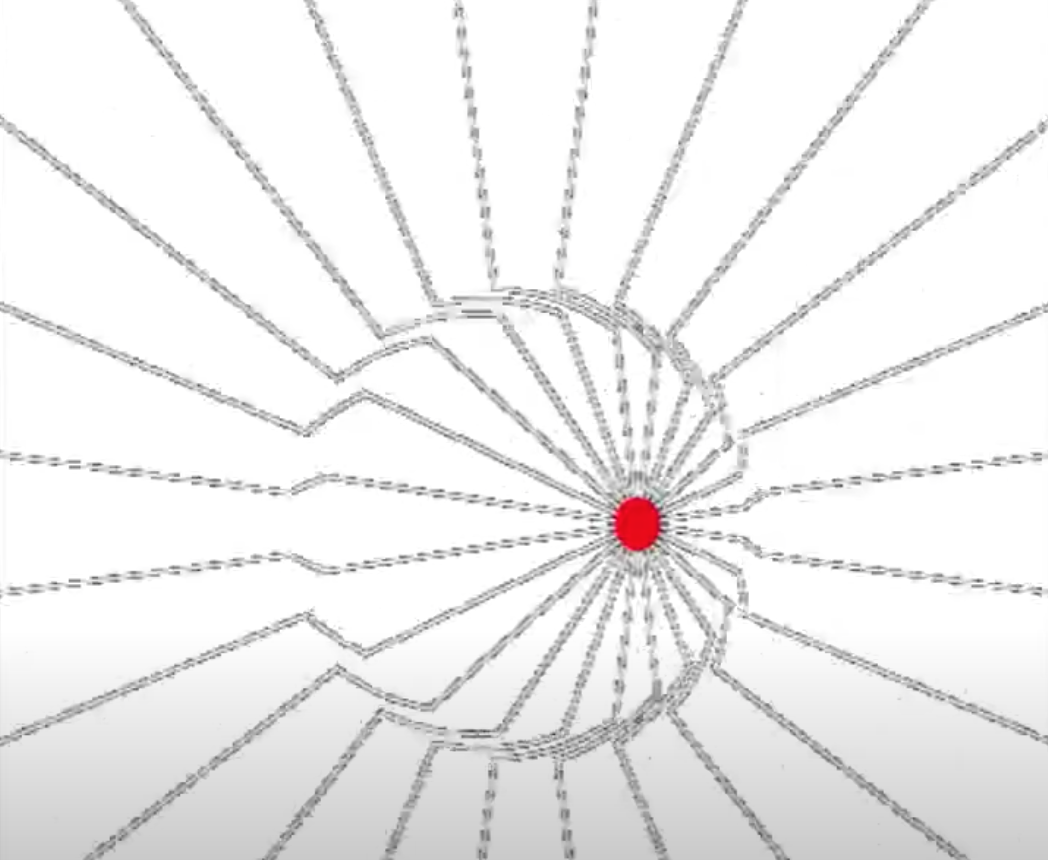
\includegraphics[width=0.66\textwidth]{figures/Screen Shot 2020-09-02 at 10.45.56 PM.png}
    \caption{}
    \label{fig:no}
\end{figure}

What is the power radiated in that shell? We need to find the perpendicular and radial components of the $E$ field in that region. This gives us the slope of the $E$ field there. 

\begin{equation}
    \frac{E_\perp}{E_r} = \frac{\Delta v t \sin{\theta}}{c \Delta t} = \frac{ar}{c^2} \sin{\theta}
\end{equation}

We also know:

\begin{equation}
    E_r = \frac{q}{r^2} \rightarrow E_\perp = \frac{qa \sin{\theta}}{c^2 r}
\end{equation}

We can use the energy density in the EM field, and we also know that $E^2 = B^2$. Therefore, 

\begin{equation}
    U = \frac{E^2}{ 4 \pi} \rightarrow E = VU = \frac{E_\perp^2}{4\pi} \underbrace{4\pi r^2 c\Delta t}_{\text{volume of shell}}
\end{equation}

The energy is thus:

\begin{equation}
    E = \frac{q^2 a^2}{c^4 r^2} \times \overbrace{\frac{1}{4\pi} \int \sin^2{\theta} d\theta}^{\text{average of sine squared over shell}} \frac{1}{4\pi} c\Delta t
\end{equation}

We then get:

\begin{equation}
    E = \frac{2q^2 a^2}{3c^3} \Delta t \rightarrow \boxed{P = \frac{2}{3} \frac{q^2 a^2}{c^3}}
\end{equation}

This is the \textbf{Larmor formula}. This is the total power radiated from an accelerating charge. Remember that power \textbf{not isotropic} and we also said nothing about the frequency of the plane wave. This is because the spectrum of the emission depends on the time variation of the emission. We do not know what the energy in each photon is, but only the total power radiated. 

Interestingly, one can derive the Larmor formula another way as well. Consider a charge $q$ oscillating within a one dimensional quantum harmonic oscillator (characterized by oscillator frequency $\omega$). Further suppose that the charge starts out in an energy eigenstate $|n\rangle$ of the oscillator, and decays by spontaneous emission to $|m\rangle$. The timescale for decay is set by the Einstein A coefficient:
\begin{equation}
A  = \frac{\omega_0^3 |\alpha|^2}{3\pi\epsilon_0 \hbar c^3}.
\end{equation}
where $\alpha \equiv q\langle n | x | m \rangle$. This matrix element can be calculated trivially using the raising and lowering operators for the SHO,. Further note that that $m = n-1$ (we're talking about \textit{decay}), so we have: 
\begin{equation}
\alpha = \sqrt{\frac{\hbar}{2m\omega}}\delta_{m, n-1} \hat{x}.
\end{equation}
The energy levels of the SHO are $E_n = (n+\frac{1}{2})\hbar\omega$. Therefore, the frequency of the emitted photon as the system decays is:
\begin{equation}
\omega_0 = \frac{E_n - E_m}{\hbar} = \omega.
\end{equation}
So, the emitted photon has a frequency which is equal to the oscillation frequency of the system! We can also calculate the lifetime of the state, $\tau \sim 1/A$:
\begin{equation}
\tau = \frac{6\pi\epsilon_0mc^3}{nq^2\omega^2}.
\end{equation}
The \textit{power} carried away is just the energy carried away divided by this timescale, i.e.:
\begin{equation}
P = \frac{q^2\omega^2}{6\pi\epsilon_0mc^3}n\hbar\omega = \frac{q^2\omega^2}{6\pi\epsilon_0mc^3}(E_n - \frac{1}{2}\hbar\omega)
\end{equation}
Dropping the $\frac{1}{2}\hbar\omega$ (this is the classical limit, $\hbar \rightarrow 0$), and using the fact that $E = \frac{1}{2}kx^2 = \frac{1}{2}m\omega^2x^2_0$, we have:
\begin{equation}
P =  \frac{q^2\omega^4x_0^2}{12\pi\epsilon_0c^3}.
\end{equation}
Finally, we note that for a harmonic oscillator, differentiating $x(t)$ twice and time averaging gives us an acceleration $\langle a^2 \rangle = x_0\omega^2/2$. So, our expression above is just:
\begin{equation}
P =  \frac{q^2a^2}{6\pi\epsilon_0c^3},
\end{equation}
which is exactly the classical Larmor formula!


\subsection{Fourier Transform}

The Fourier Transform changes something from time domain to frequency domain and back again (using the inverse FT). 

\begin{equation}
    F(\omega) = \int_{-\infty}^{\infty} f(t) e^{i \omega t} dt
\end{equation}

We can express any signal as a sum of sine waves with some frequency and amplitude. The Fourier transform takes in the signal and outputs the amplitude as a function of $\omega$. You get both a real and imaginary part, too, for both the amplitude of the cosine and sine terms in the Fourier expansion.\\

\subsection{Class Notes}

The point here is to connect what we might be familiar with to higher level abstractions like specific intensity. At the highest level of abstraction, we are considering something delivering energy over time per Herz per frequency per area, etc. Also, note that the ``derivation'' of the Larmor radiation above is a bit hand-wavy.  

This interactive simulation illustrates how, in the non-relativistic regime,
accelerating a charged particle at a characteristic frequency $\nu$ launches
oscillations in the electric field that propagate outward as an electromagnetic
wave.

The power radiated by an accelerated charge (integrating over all angles) follows the Larmor formula:
\begin{equation}
P = \frac{2}{3}\frac{e^2 a^2}{c^3},
\end{equation}
where $e$ is the charge of the particle, $a$ is the magnitude of the acceleration, and $c$ is the speed of light.

However, as the simulation shows, more power is radiated in directions perpendicular to the axis of acceleration.
This effect can be understood as the projection of the acceleration perpendicular to the field line connecting the charge to the observer. The Poynting Flux for any chosen direction is given by:
\begin{equation}
\frac{\vec E\times\vec B}{4\pi}c=e^2a^2\frac{\sin^2\theta}{4\pi r^2},
\end{equation}
where $E$ and $B$ are the electric and magnetic fields, respectively, $\theta$ is the angle of the chosen direction relative to the axis of the acceleration vector $\vec a$,
and $r$ is our distance from the radiating charge.

Because the acceleration dictates the axis along which the electric field is perturbed, Larmor radiation
is generally polarized, though if an ensemble of charged particles experience accelerations in different
directions, the ensemble averaged radiation may be depolarized.\\


Why can we think of Larmor radiation of a photon? We are mostly classical, except for when it is absolutely necessary to do quantum. We cannot know the momentum or energy of a photon, or it's direction, perfectly. We have HUP for a reason. You can think of these photons as bundles of energy. You will not find a photon along the axis, and more and more likely to find a photon perpendicularly. 

I also note here that this is a non-relativistic derivation. Later, we will go to the relativistic Larmor derivation. 

We did an activity where we talked about the impedance of free space. The impedance of free space it $Z = 377 \Omega$. You need to integrate electric field over a distance to get an $emf$, which is a voltage. Therefore, an $\vec{E}$ field is like a voltage per unit distance. This turns $\vec{J}$ to a current per unit surface area. This is equivalent to chopping up space into cubes. Once you start doing everything in terms of volumes, the densities work really well with electric fields and voltages. \\

\textbf{Feynman Disk Paradox:}\\

Maybe you've heard this one.  Suppose you have a superconducting cylindrical 
disk (think DVD) with $N$ spheres of charge $q/N$ attached around the perimeter.
The disk is constrained to be able to rotate axially around its center.  We
will call this the $\hat z$ axis.

Superconductors can have magnetic fields frozen in, and this disk does, with
$\vec B=B_0\hat z$.  Suppose the disk is allowed to warm up and stop 
superconducting, so that this magnetic field dissipates.  The change in $\vec B$
must induce a curl in the electric field, which will drive the charges
around the perimeter of the disk in a circle, setting the disk spinning.
The spinning disk now has angular momentum where it previously did not.  We
know angular momentum is conserved, so where did it come from?\\

\textbf{Solution}:\\

The angular momentum comes from the energy stored in the magnetic field. But that's not an angular momentum! Because photons have an angular momentum (they are bosons and have integer angular momentum). So the electric and magnetic fields (photons) impart angular momentum to the disk. \textbf{The angular momentum was in virtual photons, swirling around the disk, stored in the magnetic field. As this went away, the angular momentum was transferred to the disk.}\\

\textbf{Dipole Spin-Down}:\\

Suppose I have an electric dipole $\vec d$ consisting of two charges $q$ and $-q$, each of mass $M$, separated by a vector $\vec r$, and this dipole is spinning around its center of mass with an angular frequency $\omega$ in a direction orthogonal to the dipole.

How does the slow-down time (say, the "half-life" or the time it takes the rotor to lose half its rotational energy) scale with $\omega$ and $q$?\\

\textbf{Solution:}\\

We can show that $t \propto \frac{E}{P} \propto \frac{1}{(q\omega)^2}$.

%%%%%%%%%%%%%%%%%%%%%%%%%%%%%%%%%%%%%%%%%%%%%%%%%%%%%%%%%%%%%%%%%%%%%%%%%%%%%%
%%%%%%%%%%%%%%%%%%%%%%%%%%%%%%%%%%%%%%%%%%%%%%%%%%%%%%%%%%%%%%%%%%%%%%%%%%%%%%
%%%%%%%%%%%%%%%%%%%%%%%%%%%%%%%%%%%%%%%%%%%%%%%%%%%%%%%%%%%%%%%%%%%%%%%%%%%%%%
\newpage
\section{September 8, 2020: Scattering and Absorption}

\subsection{Basic Scattering:}

We describe radiation passing through a medium with specific intensity, and we use radiative transport to describe how $I_\nu$ changes as a function of distance $s$. This is a function of emission $j_\nu$ and extinction $\alpha_\nu$. 

We now talk about scattering as a special case about radiative transfer. Scatters displace photons out of line-of-sight or placing a photon \textit{into} our line-of-sight. Scatting can remove or add photons, basically. Scattering is \textit{like} emissivity, but it depends on the ambient radiation -- that is to say, if we have a scatterer, light from all directions can be scattered into line of sight. Therefore we care about the cross section of scattering the light from all directions, which itself could be a function of $\hat{n}$ direction.

The total light will thus be the integral times the cross section for that direction, making sure to have the right units (to get the units to work, we divide out by the total solid angle, and divide by the volume -- think about it, scattering likely depends on the number density of scatterers):

\begin{equation}
    j_{\nu,\text{scattering}} = \frac{n_{\text{scatterers}}}{4\pi}\int I_\nu (\hat{n}) \sigma_\nu (\hat{n}) d \Omega 
\end{equation}

We can make this a little more intuitive by the simplifying assumption that the scattering cross section is not direction dependent:

\begin{equation}
    j_{\nu,\text{scattering}} = n \sigma J_\nu
\end{equation}

where

\begin{equation}
    J_\nu \equiv \frac{1}{4\pi}\int I_\nu(\hat{n}) d \Omega
\end{equation}

\subsection{Central Limit Theorem}

Let $x_1,x_2,\dots,x_n$ be a set of $n$ independent random variables drawn from some distribution that need not be Gaussian, with each $x_i$ distributed around a mean value $\mu_i$ with a finite variance $\sigma_i^2$.  Then
the variable
\begin{equation}
z\equiv\frac{\sum_{i=1}^n{(x_i-\mu_i)}}{\sqrt{\sum_{i=1}^n{\sigma_i^2}}},
\end{equation}
in the limit of $n\to\infty$, will have a Gaussian distribution with zero mean ($\mu=0$) and unit variance ($\sigma^2=1$).

It turns out that the Central Limit Theorem can also hold for random variables, each drawn from a different, not-necessarily-Gaussian distribution, but only under the additional (not unreasonable) condition that at least one higher order moment of the distribution of the ensemble converges to zero.

\subsubsection{Implications}

There are two big implications of the Central Limit theorem:
\begin{enumerate}
\item Ensembles of many random processes/variables converge to Gaussian distributions.  That's why normal distributions are everywhere.
\item When adding together random numbers, the variance of the sum is the sum of the variances of those numbers.
\end{enumerate}
Statement 2 is important.  It means that, if you are averaging a bunch of samples drawn from the same distribution (e.g. they are all measurements with the same random error):
\begin{equation}
\bar x = \frac1n\sum_{i=1}^n{x_i}
\end{equation}
then the standard deviation of $\bar x$ (which you'd see if you computed this average with new random samples over and over again) decreases as the square root
of the number of samples averaged:
\begin{equation}
\sigma_{\bar x} = \frac{\sigma_x}{\sqrt{n}}
\end{equation}
That's why you get a better estimate of a quantity by making lots of (independent) measurements.  But you only do so as the square-root of the number of measurements.

\subsection{Random Walks}

We can imagine a drunk person stumbling along, takes steps, stumbles and changes direction, taking steps in new random directions. This is in contrast to our usual understanding of random processes where we draw points. In the random walk, we chain random numbers together.

Suppose $\phi$ is a random variable. Let $\vec{\phi} = \phi_0, \phi_1, \phi_2,...$ be a collection of random numbers. A random walk is the sum of these variables $\vec{w}$ where $w_j = \sum_{j=0}^{i} \phi_j$. There are plenty of examples of random walks, from games in a series (sports), diffusion, scattering processes (like Plinko from Price Is Right), statistical model fitting (Markov Chain Monte Carlo [MCMC] simulations!), and more. 

What are some properties of random walks? First, if $\langle \phi \rangle = 0$, then $\underbrace{w_i - w_j}_{\text{curr. - prev. location}} \propto \sqrt{i-j}$. Another way of saying this is that the sum of $N$ random numbers with random mean is is $\sqrt{N}$. This means that \textbf{random numbers add in quadrature} (on average). This comes from the fact that the two steps often are in two dimensions, not in a single dimension (because the random numbers are uncorrelated). 

One effect of this is to consider a series of measurements $p$ with noise $\phi_i$:

\begin{equation}
    \frac{1}{N} \sum_{i=1}^{N} p+\phi_i = \hat{p} + \frac{1}{\sqrt{N}\langle |\phi|\rangle}
\end{equation}

For example, diffusion times are proportional to distance squared. Also, even though the sum of random numbers is proportional to $\sqrt{N}$ does not depend on dimensionality, the \textbf{timescale} does. Think -- there is more and more volume to explore in higher dimensions. There are more steps in completely different directions.

\subsection{Random Walks inside a Star}

Radiative energy transport inside stars can be approximated as a random walk, where a photon gets repeatedly absorbed and re-emitted in a random direction as it tries to make it way out of through the stellar interior. The step length of this random walk is equal to the mean free path $\lambda$. For the sun-type star, $\lambda \sim 10^{-2}$ cm. The number of steps required to reach the stellar radius r is, $N = (r/\lambda)^{2}$. For the sun, $r \sim 10^{11}$ cm, so $N \sim 10^{26} $ steps. In each step, light travels approximately a distance $\lambda$. Therefore by the time the photon reaches the surface it has traveled $\sim N \times \lambda = 10^{24}$ cm. At the speed of light, that would take $\sim 10^{7}$ years! 

The figure below shows a simulation of a random walk process inside a hypothetical star of radius 10 cm. Why such a small star? If my (non-super) computer runs through $10^{6}$ random walk steps in a second, then it would take $10^{20}$ seconds to complete the random walk of a single photon moving through the entire sun's radius. That is twice the age of the universe! I doubt I can get an extension on this project for that long. 

\begin{figure}[h!]
    \centering
    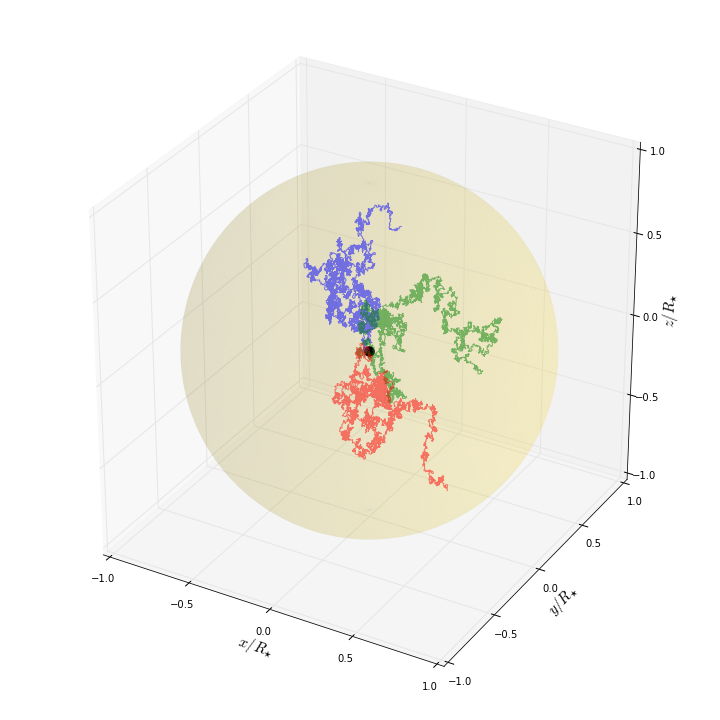
\includegraphics[width=0.5\textwidth]{figures/Random_walk.png}
    \caption{}
    \label{fig:random_walk}
\end{figure}

\subsection{Statistical Degeneracy}

What makes some outcomes more probable than others? A better question -- where should you build hotels in Monopoly? When you roll 2 die, you get the convolution of the two distributions, giving you the triangular distribution. At the center of this distribution is 7 since there are 6 ways to add two die to give 7 (which is maximal). Next best is 6 and 8.

But what makes some outcomes more probable than others? The number of ways of generating that outcome. This is \textbf{degeneracy}. We also use the terminology ``the number of microstates in a macrostate.'' There are 6 ``microstates'' that we group under the macrostate we call ``7.'' All of probability comes down to counting the degeneracy of outcomes. For example, a straight flush is worth more than straights or flushes, since it's the intersection of two low-probability outcomes (degeneracies). 

The hard part is -- what do you count? Consider two decks of cards, a blue and a green deck. What is the chance of getting a straight flush:

\begin{equation}
    \frac{\text{straight flush (blue) + straight flush (green)}}{\text{all (blue) + all (green)}} = \frac{2\text{straight flush (blue)}}{2\text{all}} 
\end{equation}

The degeneracy of the cards do not count! One last thing about degeneracy...the Boltzmann equation relates the number of particles in a state to the energy of that state. How do we actually calculate that degeneracy $g_i$? In this equation, $g_i$ is a count of microstates for the macrostate $E_i$. Also, degeneracy \textbf{does} account for all the variation in probability of $n$. That is to say that $e^{-E_i /k T}$ is a second degeneracy term. We can think of this as $kT$ being an energy bar of the system. We then chop this energy bar into pieces and give it to each particle. We also make sure that there are more chunks of energy than particles, and also that some particles get no energy. 

What are the consequences? One example configuration is all equal amounts of energy. How many rearrangements are there of this? Every shuffling of the energy is the exact same configuration. This is all to say that there is only one configuration where they all have the same energy.

What about half particles getting 0, and the other half getting twice that initial energy? The only rearrangements that matter there are exchanges between groups of particles. Counting those rearrangements, we get:

\begin{equation}
    \frac{N!}{(N/2)!(N/2)!}
\end{equation}

We can generalize this to multiply groups:
\begin{equation}
    \frac{N!}{A! (N-A)!} \frac{(N-A)!}{B! (N-A-B)!}
\end{equation}

Where we can keep adding similar terms. If we keep subdividing on and on, we get a bunch of cancellations. This gives us ($i$ ranging over all groups):

\begin{equation}
    \text{Total Arrangements} = \mathcal{G} = N! \prod_i \frac{1}{N_i!}
\end{equation}

We also invoke \textbf{Stirling's Approximation:} $N! \approx N^N e^{-N}$. We lastly want to find the arrangement that maximizes $\mathcal{G}$. This gives us the mostly likely state. To maxmimize $\mathcal{G}$, we should maximize that natural log of $\mathcal{G}$: $\ln \mathcal{G}$ since this is easier. One last thing is to account for additional degeneracies that might account for other intrinsic properties. We then use Fermat's Theorem of Stationary Points. This, all together, gives us:

\begin{equation}
    \ln \mathcal{G} \approx \sum_{i=1}^n N_i \ln g_i - N_i \ln N_i + N_i
\end{equation}

We also normalize for the total amount of energy $kT$. We also use boundary condition: $\sum_{i} N_i E_i = NkT$. We would then get:

\begin{equation}
    n_i \propto g_i e^{-E_i/kT}
\end{equation}

Where the exponential comes from Stirling's approximation. 




\subsection{Class Notes}

A very basic way to think about degeneracy. Degeneracy is the number of ways of getting the same state that you are counting. Sometimes we call it the number of microstates in a macrostate. An obvious example of this is rolling two sets of dice. What is the most likely cumulative roll? Of the $36$ possible rolls, $6/36$ will add to $7$, making it the most likely roll. 

The art of degeneracy is what the heck do we actually count? We can have coins, we can have die, but what about the number of spin states in an electron that are indistinguishable? Similarly, doing a black-body derivation, you count the total number of ``momentum-states'' with equal energy, so the momenta are ``microstates'' and energy is the ``macrostate.'' We then will start using the Boltzmann Equation talking about the $i$th state with degeneracy $g_i$ and energy $E_i$:

\begin{equation}
    n_i \propto g_i \underbrace{e^{-\frac{E_i}{k_B T}}}_{\text{this comes from literally counting using Stirling's approx.}}
\end{equation}

\subsection{Class Notes}

``I always find random walks in life.''

\subsubsection{What is the emissivity of an ideal scatterer in the absence of ambient light?}

In the absence of ambient light, the emissivity is $0$ since it has nothing to scatter.  Remember that we have:

\begin{equation}
    j_{\nu, \text{scattering}} = n \sigma_\nu J_\nu
\end{equation}

where:

\begin{equation}
    J_\nu = \frac{1}{4\pi} \int I_\nu d\Omega
\end{equation}

can be thought of as the averaged over all angles specific intensity. We therefore have $J_\nu = 0$, cancelling $j_{\nu, \text{scattering}}$ from our radiative transfer equation.

What does it mean to be an ideal scatterer?
\begin{itemize}
    \item No absorption $\rightarrow$ energy conserved (elastic)
    \item Isotropic scattering.
\end{itemize}

\subsubsection{One-hundred Coin Flips}

Suppose I flip a coin 100 times and record the number of heads $H$ and the number of tails $T$. What is the expected value of $\sqrt{\langle (H - T)^2\rangle}$?


\begin{lstlisting}
import numpy as np

data = np.where(np.random.uniform(0, 1, size=(100000, 100)) < 0.5, -1,1)

print(np.sqrt(np.mean(np.sum(data, axis = 1)**2)))
\end{lstlisting}

The answer turns out to be $10$. Why is that the case? Well we have $\langle H - T\rangle$ as a random variable. When we do a single flip, we have $(H-T)^2 = 1$. When we do two flips, our average should be $2$. \textbf{Our variance is growing linearly with number of flips}. This is another statement of a the central limit theorem. As we go to more an more flips, $\langle (H-T)^2 \rangle$ grows linearly with flips. At $100$ flips, we have $\sqrt{100} = 10$. Note, however, for 100 flips:

\begin{equation}
    \langle H - T \rangle = 0
\end{equation}

whereas:

\begin{equation}
    \sqrt{\langle (H-T)^2 \rangle} = 10
\end{equation}




%%%%%%%%%%%%%%%%%%%%%%%%%%%%%%%%%%%%%%%%%%%%%%%%%%%%%%%%%%%%%%%%%%%%%%%%%%%%%%
%%%%%%%%%%%%%%%%%%%%%%%%%%%%%%%%%%%%%%%%%%%%%%%%%%%%%%%%%%%%%%%%%%%%%%%%%%%%%%
%%%%%%%%%%%%%%%%%%%%%%%%%%%%%%%%%%%%%%%%%%%%%%%%%%%%%%%%%%%%%%%%%%%%%%%%%%%%%%
\newpage
\section{September 10, 2020: Thermodynamic Equilibrium}

\subsection{Black-body Radiation and Kirchoff's Law}

A blackbody is the simplest source: it absorbs and re-emits radiation with
100\% efficiency.  The frequency content of blackbody radiation is given by
the {\it Planck Function}:

\begin{equation}
\boxed{B_\nu = \frac{2h\nu^3}{c^2}\frac1{e^\frac{h\nu}{k_B T}-1}}
\end{equation}


Electromagnetic radiation can always be traced to accelerated charges. For example, consider de-excitation of electron states or deflection of charges in EM field (brehmsstrahlung) or random ``Brownian'' motion like atoms colliding in a gas. The electron shells oscillate thermally, and gives us a photon $E \propto T^{P}$. \textbf{Black-body radiation} is radiation only due to Brownian motion. 

We will be concerned with two quantities for black-body radiation:

\begin{equation}
    [u(\nu,T)] = \frac{\text{Energy}}{\text{volume}\times \text{frequenecy} \times \text{steradian}}
\end{equation}

\begin{equation}
    u_{\text{tot}}(T) = 4\pi \int_0^{\infty} u(\nu,T)  \mathrm{d}\nu 
\end{equation}

We can make a naive guess before Planck and Einstein. If we look at units of our energy distribution, we can plug in $k_B T$ for energy, and use dimensional analysis on other quantities of light (frequency and speed):

\begin{equation}
    u(\nu,T) = \underbrace{2}_{\text{two pol. states}} \times \frac{ k_B T \nu^2 }{c^3}
\end{equation}

If we integrate the naive guess, we obtain:

\begin{equation}
    u_{\text{tot}}(T) = \infty \rightarrow \text{UV catastrophe}
\end{equation}

We now consider a quantum description. COnsider a box of fixed length $L$ and temperature $T$. The box has perfectly reflecting walls, acting as boundary conditions. In practice, this means that $n_i\lambda_i = 2L$ and $k_i = \frac{2\pi}{\lambda_i}$. This gives us:

\begin{equation}
    |\vec{k}| = \frac{\pi^2}{L^2} \left( l^2 + m^2 + n^2 \right) \rightarrow \left(\frac{\pi p }{L}\right)^2
\end{equation}

where $p$ is defined for convenience. We now heat to $T$, causing chages to oscillate and produce thermal radiation. The quantity we want is the density of thermal radiation inside the box:

\begin{equation}
    u = n(\nu) \times \bar{E}(T)
\end{equation}

Let's start with $n(\nu)$. We want number of oscillators in a little $d\nu$:

\begin{equation}
    \nu = \frac{c}{\lambda} \rightarrow \frac{cp}{2L} \rightarrow d\nu = dp 
\end{equation}

We can then integrate over $p$ and go back to frequency, integrating over a shell. We also need $k = \omega c$. This eventually gives

\begin{equation}
    n(\nu) = \frac{N(\nu)}{V} =  \frac{8 \pi \nu^2}{c^3}
\end{equation}

We can now go get $\bar{E}(T)$. The average energy of a thermal oscillator is $k_B T$, so classically we have:


\begin{equation}
    u(\nu, T) = \frac{N(\nu)}{V} =  \frac{2 \nu^2}{c^3} kT
\end{equation}

Now, we need quantum mechanics. What's the average specific energy of a QM oscillator? We have:

\begin{equation}
    E = nh\nu
\end{equation}

Additionally, because we are in thermodynamic equilibrium, giving us maximum entropy and therefore, we can use the Boltzmann distribution from statistical mechanics:

\begin{equation}
    p(E_N) = \frac{e^{-\beta E_N}}{\sum_N e^{-\beta E_N}}
\end{equation}

We eventaully get:

\begin{equation}
    \bar{E}_\nu = \frac{h \nu}{e^{\beta h \nu} -1}
\end{equation}

We now have:

\begin{equation}
    u = n(\nu) \times \bar{E}(T)
\end{equation}

\begin{equation}
    \boxed{u(\nu, T) = \frac{2 h \nu^3}{c^2} \frac{1}{e^{\frac{h\nu}{k_B T} - 1}}}
\end{equation}

\begin{equation}
    \boxed{[u(\nu, T)] = \frac{\ergs}{\text{volume}\times\hz\times\sr}}
\end{equation}

We can now calculate the integral over all frequencies, giving us the total energy radiated by a black-body (let $x \equiv \frac{h\nu}{k_B T}$:

\begin{equation}
    u_{\text{tot}}(T) = \frac{2 h}{c^3}\left(\frac{k_B T}{h}\right)^4 \underbrace{\int_0^\infty \frac{x^3}{e^x -1} \mathrm{d} x}_{\pi^4/15}
\end{equation}

\begin{equation}
    u_{\text{tot}} = \frac{2\pi ^4 k_B^4}{15 c^3 h^3 } T^4 = \sigma T^4 
\end{equation}

\begin{equation}
    \boxed{u_{\text{tot}} = \sigma T^4}
\end{equation}

So how does the naive guess hide in the quantum mechanic derivation? Take the limit $h \nu \ll k_B T$. We can then expand $e^x$ to first order, recovering the classical limit of the black-body function. This is called the \textbf{Rayleigh} limit, or the limit for long wavelength. It is also so common in astronomy that we can use it to make brightness temperature maps of the night sky or of emission regions. 

\subsection{Formal Derivation}

If you take Bose-Einstein statistics as a given, deriving the Planck function is pretty straightforward; it boils down to counting degenerate states for a given energy.

To begin with, we need to relate the specific intensity of radiation from a blackbody, $B_\nu$, to an energy density that we can then count up states for:
\begin{equation}
\frac{4\pi}{c}B_\nu=D_\nu\cdot f(\nu)\cdot E,
\end{equation}
where $D_\nu$ counts up the specific degenerate states per volume for a given energy, $f(\nu)$ is the probability
of occupying that energy, and $E$ is the energy of that state.  Hence, the right side of this equation expresses specific energy density.  On the left side,
since $B_\nu$ has units of ${\rm ergs}/{\rm s}\cdot{\rm Hz}\cdot{\rm cm^2}\cdot{\rm sr}$, dividing by $c$ converts the specific flux to a specific
energy density, with units of ${\rm ergs}/{\rm Hz}\cdot{\rm cm^3}\cdot{\rm sr}$ (recall "specific" means "per frequency").  The factor of $4\pi$ comes
from assuming isotropic emission, and cancels out the factor of ${\rm sr}$.

For energy, we can use $E=h\nu$, and assuming Bose-Einstein statistics (photons are bosons, after all), we have that $f(\nu)= 1/(e^\frac{h\nu}{kt}-1)$.
All that remains is to figure out $D_\nu$, the number of degenerate states per volume per frequency for a given energy.  To do this, let's
examine a cube of space with length $L$ on a side.  For a finite region of space, the energy states a photon can take are quantized.  This is because, to be occupied in this volume, a photon go through an integral number of wavelengths in distance $L$ along each of the $\hat x, \hat y$, and $\hat z$ axes.  An equivalent way of saying this is that frequency comes in units of $c/L$.  

So if we want to count the number of degenerate states that all have the same energy for some differential frequency interval $d\nu$, we can calculate
that by calculating the volume these states occupy in phase space.  Since $E=h\nu$, the surface area of a shell of constant energy is $4\pi\nu^2$,
and since each quantized state occupies a volume $(c/L)^3$ is phase space, the total number of states is given by:
\begin{equation}
D_\nu\cdot V\cdot d\nu= \frac{4\pi\nu^2d\nu}{(c/L)^3}\cdot g,
\end{equation}
where the volume $V=L^3$, and $g=2$ is a final degeneracy factor that accounts for the fact that photons can have 2 different polarizations.

Working out the algebra and plugging everything into our original equation for $B_\nu$, we end up with:
\begin{equation}
B_\nu = \frac{2h\nu^3}{c^2}\frac1{e^\frac{h\nu}{kT}-1}
\end{equation}

\subsection{Kirchoff's Law}

Kirchoff's Law is a statement that may alternately be regarded as obvious or deeply insightful.  Simply put, it
states that, for an object in a (let's say, Planckian) radiation bath in thermal equilibrium, the energy absorbed
equals the energy radiated.  As obvious as this may seem, Kirchoff's Law can have non-obvious implications.
For example, let's take the equation for Radiative Transport:
\begin{equation}
\frac{dI_\nu}{ds}=j_\nu - \alpha_\nu I_\nu.
\end{equation}
In the optically thick limit for blackbody radiation, $I_\nu=B_\nu$ and $dI_\nu/ds=0$.  Hence,
\begin{equation}
j_\nu=\alpha_\nu B_\nu(T).
\end{equation}
On one level, this is simply saying that for a medium in local thermodynamic equilibrium, $S_\nu\equiv j_\nu/\alpha_\nu = B_\nu(T)$.  But on another level, since the values of $j_\nu$ and $\alpha_\nu$ are inherent properties of a medium and don't depend on thermal equilibrium, this is a fundamental relationship between $j_\nu$ and $\alpha_\nu$.   Kirchoff's law says that good emitters are good absorbers, and vice versa.

This fundamental relationship between $j_\nu$ and $\alpha_\nu$ ensures that, when things are brought into thermal equilibrium, the resultant
spectrum is always Planckian, and does not depend on the emissivity or absorptivity of the medium.

\subsection{Sources of Black-body Radiation}

There are not many examples of true blackbody sources of radiation, but what few there are tend to be quite important.

\subsubsection{Cosmic Microwave Background}

The mother of all blackbodies, this is the relic 2.7K radiation left over from the hot plasma that was generated by the Big Bang.  Photons were produced and absorbed via the thermal radiation of charged particles (mostly electrons) scattering off one another, converging quickly on a blackbody spectrum.  Once the universe cooled to the point that protons and electrons could bind to form neutral hydrogen without being immediately ionized, these photons stopped scattering, and have been free-streaming ever since.  As the universe expands, the wavelength of these photons stretch with it, causing photon energies (and hence, the characteristic temperature) to gradually decline with time.  Note that, at the current temperature of 2.7K, the CMB peaks at 160.2 GHz.

\subsubsection{Sun}

Stars are generally blackbody-like, although most of them are so faint in the radio band as to be nearly unobservable.  Just by sheer proximity, our Sun is the brightest radio source in the sky, but, particularly at lower frequencies, not by a huge margin. Emission from the quiet Sun is dominated at radio frequencies by the photosphere (6000K) around 100 GHz, the chromosphere (10,000K) at 1 GHz, and the  corona (1,000,000K) at 100 MHz.  As a result, the spectrum of the quiet Sun within a relatively narrow band is blackbody-like, but broadly departs from the characteristic blackbody spectrum.

It should also be noted that during sunspot activity, which varies on an 11-year solar cycle, solar emission departs dramatically from that of a blackbody, and becomes dominated by intense emission from electrons trapped in the magnetic fields around sunspots.  The perturbed sun can be orders of magnitude brighter than the quiet Sun, and with emission dominated by particular ``hot spots'' that rotate with the Sun.


\subsection{Boltzmann Distribution}

The Boltzmann distribution gives the relative fraction of atoms in two states in thermal equilibrium at a certain temperature, taking into account the degeneracies of these states and the energy difference between states. This distribution applies to large ensembles of atoms such that statistical arguments are valid. The formula for the Boltzmann distribution is given by the following:

\begin{equation}
\boxed{\overbrace{\frac{n_2}{n_1}}^\text{\# of molecules  in upper level over lower level}=\underbrace{\frac{g_2}{g_1}}_{\text{ratio of degeneracies}} \times \underbrace{e^{-\frac{\Delta E}{kT}}}_{\text{Boltzmann factor}}}
\end{equation}

where $n_1,n_2$ are the number (or number density) of atoms in energy states 1 and 2, respectively, $g_1,g_2$ are the respective degeneracies of those energy states (i.e., how many distinct configurations of the atom have that same energy state), $\Delta E=E_2-E_1$ is the energy difference between the two states, $k$ is Boltzmann's constant, and $T$ is the temperature describing the distribution of states in the system.

Note the distinction between the Boltzmann distribution, which describes the distribution of energy states in the system at a given temperature, and the Maxwell-Boltzmann distribution, which instead describes a distribution of velocities at a given temperature.

The Boltzmann distribution tells us which transitions to expect from a population, since, for a transition to occur, we must begin with particles in the starting state such that they may transition to the end state. Together with the Saha Equation, it can also tell us the ratio of element abundances in stellar astrophysics, allowing for the interpretation of stellar spectra.

\subsubsection{Derivation}

Consider an isolated statistical ensemble of N particles with energies given by

$$E = \sum \epsilon_i n_i$$

and total number of particles

$$N = \sum n_i.$$

The N particles are arranged into microstates given by

$$W = (g_1^{n_1} g_2^{n_2} g_3^{n_3} ...)\frac{N!}{n_1!n_2!n_3! ...}.$$

Here, W is the probability of a given distribution. To find the distribution of particles in our system, we will need to find the most probable microstate, or the distribution that maximizes W. To accomplish this, we will equivalently find a maximum in lnW.

Solving for lnW from our previous expression, we get

$$\ln W = n_1 \ln g_1 + n_2\ln g_2 + ... + \ln N! - n_1\ln n_1 - n_2\ln n_2 - ... + n_1 + n_2 + ...$$
$$\ln W = n_1(1 + \ln \frac{g_1}{n_1}) + n_2(1 + \ln \frac{g_2}{n_2}) + ... + \ln N!$$

where we implemented Stirling's approximation for large N, $\ln N! \approx N \ln N - N$, to simplify our expression. Using Lagrange's method of undetermined multipliers, we seek a maximum in

$$ \ln W - \alpha \sum n_i - \beta\sum\epsilon_in_i, $$

where $\alpha$ and $\beta$ are constant values. A maximum in this expression is equivalent to a maximum in lnW or in W because the second and third terms consist of only constant values, where we have defined our total energy and our total number of particles to be constant (recall that we are considering an isolated ensemble). Thus, we solve for the maximum value of this expression with respect to $n_i$ to find the most probable microstate.

$$ \frac{d}{d n_i} (\ln W - \alpha \sum n_i - \beta\sum\epsilon_in_i) = \frac{d \ln W}{dn_i} - \alpha - \beta\epsilon_i = 0 $$

Recalling our equation for $\ln W$ from earlier, 

$$ \frac{d\ln W}{dn_i} = \frac{d}{dn_i}(n_i + n_i \ln g_i - n_i \ln n_i) $$
$$ \frac{d \ln W }{dn_i} = 1 + \ln g_i - \ln n_i - n_i\frac{1}{n_i} $$
$$ \frac{d\ln W}{dn_i} = \ln \Big(\frac{g_i}{n_i}\Big) $$

Plugging this in to our maximum probability expression, we then get

$$ \ln\Big(\frac{g_i}{n_i}\Big) - \alpha - \beta\epsilon_i = 0 $$
$$ \frac{g_i}{n_i}e^{-\alpha}e^{-\beta\epsilon_i} = 1 $$
$$ n_i = g_i e^{-\alpha}e^{-\beta\epsilon_i} $$

Finally, taking a ratio between two energy states, we get

$$ \frac{n_i}{n_j} = \frac{g_i}{g_j}e^{-\beta(\epsilon_i - \epsilon_j)}, $$

which is a generalized form of the Boltzmann equation. Here, $\beta = \frac{1}{kT}$. The $\alpha$ term in our derivation, though it dropped out of our Boltzmann distribution, is given by $\alpha = \frac{\mu}{kT}$, where $\mu$ is the chemical potential.

\subsubsection{Degeneracies of the hydrogen atom}

The energy degeneracies corresponding to each $E_n$ for the hydrogen atom are given by:

\begin{equation}
g_n = \sum^{n-1}_{l=0} (2l + 1) = n^2
\end{equation}

Taking the two electron spin states and the two proton spin states of hydrogen into account, our degeneracies then ultimately become

\begin{equation}
g_n = 4n^2.
\end{equation}

Using this expression for our degeneracies, we can then show the ratios of excited states of hydrogen to the ground state as a function of temperature:

\begin{figure}[ht]
    \centering
    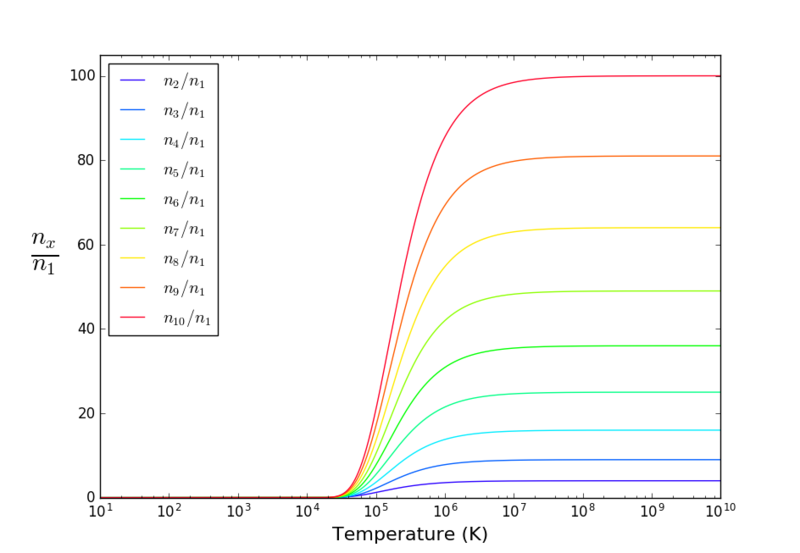
\includegraphics[width=0.66\textwidth]{figures/boltzmann.png}
    \caption{}
    \label{fig:Boltzmann}
\end{figure}

\subsection{Maxwellian Velocity Distribution}

This describes the distribution of velocities of speeds of molecules in an environment. The distribution is given by:

\begin{equation}
    \boxed{f(v) = 4 \pi \left(\frac{m}{2 \pi k T}\right)^{3/2} v^2 e^{-\frac{\frac{1}{2} m v^2}{ kT}}}
\end{equation}

We then want to understand three different velocities:

\begin{equation}
    \boxed{v_{\text{rms}} = \sqrt{\frac{3 k T}{m}}}
\end{equation}

This is the velocities that corresponds to the average kinetic energy. I note here that $m$ is the mass of a particle.

\begin{equation}
    \boxed{v_{\text{most probable}} = \sqrt{\frac{2k T}{m}}}
\end{equation}

This is the velocity that ``most'' particles have. We can do this by taking the derivative of $f(v)$ and setting it to $0$. We can the expression almost trivially, noting that the term out front is a huge constant and taking the derivative gives a huge irrelevant term:

\begin{equation}
    f(v) = C_1 \times v^2 \times e^{-C_2 v^2} \rightarrow \dots \frac{df}{dv} = -C_2 v^2 + 1 = 0
\end{equation}

\begin{equation}
    v_{\text{ave}} = \bar{v} = \sqrt{\frac{8 k T}{\pi m}}
\end{equation}

The next speed we will find is the mean speed, $\bar{v}$. To find this, we find the expectation value of $v$:
$$ \bar{v} = \int_0^{\infty} f(v) v dv = \int_0^{\infty} 4\pi \left( \frac{m}{ 2 \pi kT} \right)^{3/2} v^3 \exp\left(-\frac{mv^2}{2kT}\right) dv$$
Using the result that:
$$ \int_0^\infty x^3 exp(-x^2/a^2) = a^4/2 $$
we get:
$$\bar{v} = 4\pi \left( \frac{m}{ 2 \pi kT} \right)^{3/2} \frac{1}{2} \left(\frac{2kT}{m}\right)^2 $$

\begin{equation}
    \boxed{\bar{v} = \sqrt{\frac{8 kT}{\pi m}}}
\end{equation}

It turns out this is slightly greater than the most probably speed ($\sqrt{8/\pi} > \sqrt{2}$).

Here is a plot of typically speeds and how they compare. I note that $v_\text{rms}$ is largest, followed by the average velocity, and lastly the most probably velocity. 

\begin{figure}[ht]
    \centering
    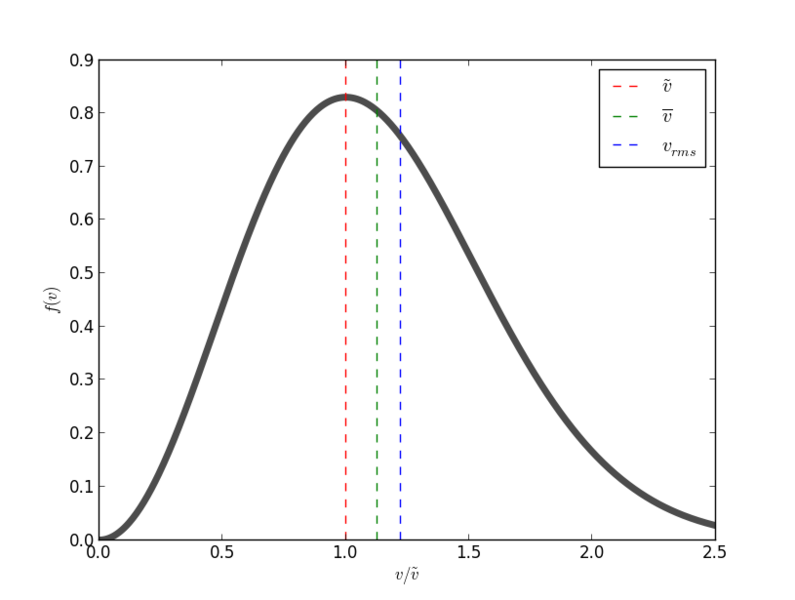
\includegraphics[width=0.6\textwidth]{figures/mbdist.png}
    \caption{Typical M-B distribution plots/values.}
    \label{fig:mwdist}
\end{figure}

\subsubsection{Applications to Planetary Atmospheres}
One application of the Maxwell-Boltzmann distribution is to describe the loss of planetary atmospheres. Particles at the top of an atmosphere are moving randomly in all directions with speeds corresponding to the Maxwell-Boltzmann distribution. If the particles moving upwards have a velocity lower than the planet's escape velocity, then the particles will curve back downwards in an elliptical pattern, and the planet will retain its atmosphere. However, if the particles moving upwards are at a higher velocity than the planet's escape velocity, then the particles will move upwards in a hyperbolic pattern and will be ejected into space. The escape velocity is given by

$$ v_{esc} = \sqrt\frac{2GM}{r} $$

where G is the gravitational constant, M is the mass of the body to escape from, and r is the distance from the particle to the center of mass of the body that it is escaping from.

Typically, only a small number of particles from the high-velocity tail of the Maxwell-Boltzmann distribution will be able to escape. However, the trajectories and speeds of the remaining atmospheric particles are continuously shuffled, leading to the gradual ejection of particles and a slow atmospheric loss. As a result of this effect, very small planets (which therefore also have very small escape velocities) are unable to retain atmospheres.

\subsection{Local Thermodynamic Equilibrium}

Thermodynamic equilibrium is the idea that you have achieved a uniform temperature $T$ in a medium, such as the temperature in a cloud. Specifically, this means that:

\begin{equation}
    \frac{\partial T}{\partial t} = \nabla T = 0
\end{equation}

\textbf{Local thermodynamic equilibrium} relaxes these assumptions. We now allow a spatially varying temperature (such as a star heating a cloud in a gradient from one side). However, in time, there is a \textit{constant} gradient. We only require:

\begin{equation}
    \frac{\partial T(\vec{x})}{\partial t} = 0
\end{equation}

Systems are vary rarely in \textbf{global} thermodynamic equilibrium, but are often in \textbf{local} thermodynamic equilibrium.

But, what do we mean by temperature? There are three ways to talk about this: 

\begin{itemize}
    \item \textbf{Kinetic temperature}: This is what we mean colloquially. This is the energy from thermal motions of molecules. This corresponds to a Maxwellian velocity distribution. You have achieved kinetic thermodynamic equilibrium when you reach Maxwell velocity distributions.
    
    \item  \textbf{Excitation temperature}: This needs to be considered when individual molecules can absorb energy and store it in an energy state. Think of a hydrogen atom holding a Lyman-$\alpha$ photon. Excitation temperatures follow Boltzmann distributions. A medium is in excitation temperature equilibrium at this point.
    
    \item \textbf{Radiation temperature}: We have talked about, previously, that $\frac{d I_\nu}{d \tau_\nu} = S_\nu - I_\nu$. In this case, the source function is given by $B_\nu$. In radiative equilibrium, we have balance at specific frequencies. \textbf{Note:} Part of local thermodynamic equilibrium is \textbf{local} in frequency -- that is to say it radiates equally at the same frequency!
\end{itemize}

In principle, these temperatures can all be different values. They can all be independent! Specific mechanisms can couple two or more of these together. For example, Doppler shifts couple to radiative and kinetic temperature. Scattering or thermal bremsstrahlung also couple these. We can couple excitation temperature and kinetic temperature with collisions between gas molecules. More collisions lead to higher excitation temperatures (and the reverse can be true -- when you have more items in a higher state, collisions can give even higher energy, driving kinetic temperature to match excitation temperature). Lastly, we can couple radiative and excitation temperature -- this is a process of photoabsorption whereby an atom or molecule absorbs a photon and stores energy. \textbf{In LTE, all of these are coupled and they all match.}

\textbf{In sum...}:

\begin{itemize}
    \item LTE couples kinetic, excitation, and radiative temperatures.
    
    \item Temperature is not time dependent but can be spatially dependent. 
    
    \item LTE is frequency dependent -- you can be in LTE at one $\nu$ but not at another. At a $\nu$ at which you are in $LTE$, $T_{rad} = T_{kin} = T_{ex}$. 
    
    \item LTE does not mean background light is attenuated, it just means the source function $S_\nu$ becomes $B_\nu$, the black-body function, at that frequency.
    
    \item Lastly, note that there has to be a reason for LTE to exist. There needs to be mechanisms to couple the three temperatures. A list of mechanisms to couple these is discussed above.
\end{itemize}

\subsection{Class Notes}

A note about the class -- everything thermal boils down to black body radiation because the source function becomes the Planck function at local thermodynamic equilibrium. You stop caring about all the specific modes of radiation. Once in equilibrium, you have \textbf{all} the distributions that correspond to that temperature. We don't care how it happens. One of the things we must determine, then, is if we are in thermal equilibrium (local). Then, we can forget crazy things and go with the Planck function. 

What prevents LTE? In dense environments, it is hard to prevent that from happening, But in space, it is often true that collisions are not cooling efficiently enough to couple kinetic energies with any of the other temperatures. You could expose a bunch of gas to light, giving a ratio to internal transitions. That ratio can be set by the light, but the collisions are not frequent enough for that to be a thermal temperature. 

It is almost impossible to be in thermodynamic equilibrium at all frequencies. Often, the underlying mechanisms and therefore the equilibria will be different. 

\textbf{In what sense is a black-body ``black''?} It is black because it reflects no light. We must realize that reflection doesn't mean no emission -- the light is it's own light, not the light from something else. This leads to an interesting question. If you weren't bathed in sunlight but you wanted to cool off, what color should you wear? It's actually \textbf{black}! Why? It is the most efficient radiator as well as a good absorptive. This comes to Kirchoff's law! If $j_\nu / \alpha_\nu = S_\nu \rightarrow B_\nu$ at LTE, this means that $j_\nu = \alpha_\nu B_\nu$. This means that the good emitters are good absorbers since $B_\nu$ is \textbf{universal}. Also, somehow everything knows to asymptote to the Planck function. But on the other hand, this comes from counting distributions of energies in boxes. It also says that emission and absorption are \textbf{deeply related} to each other. \\

\textbf{Write down the equation relation populations in different energy states in a Boltzmann distribution?} The three distributions we should know by heart are the Maxwell-Boltzmann, Boltzmann, and Maxwellian. We have Boltzmann, Planck, and MB:

\begin{equation}
    \frac{n_a}{n_b} = \frac{g_a}{g_b} e^{\frac{-\Delta E}{kT}}
\end{equation}

\begin{equation}
    B_\nu = \underbrace{\frac{2hv^3}{c^2}}_{\text{degeneracy}} \times \overbrace{\frac{1}{e^{\frac{h \nu}{kT} - 1}}}^{\sim \text{Boltzmann}}
\end{equation}

\begin{equation}
    f(v)\sim v^2 e^{\frac{-\frac12 mv^2}{kT}}
\end{equation}

\textbf{What are the conditions for LTE and what is its observable consequence?} Temperatures are not a thing by themselves, they describe a distribution. If you have all the temperatures that equilibrate, you have $S_\nu \rightarrow B_\nu$. Does that mean that $I_\nu \rightarrow B_\nu$? Not necessarily, but only if optically thick. That is to say, if you want to see the source function (Planck function), we need to see the thing that is radiating, not the thing behind it.\\

\textbf{Is the average velocity of Maxwellian the same as $\frac12 mv^2 = kT$?} No, this is the mode of the distribution. For order of magnitude, this is okay! You want to make sure you're using the right velocity if you're doing better than order of magnitude. \\

\textbf{Suppose a cloud of hydrogen starts out with all atoms moving in random directions at a uniform speed $\frac12 mv^2=kT$. Given number density $n$ and cross-section for collision $\sigma$, estimate the amount of time required to relax to a Maxwellian distribution.} We can first get a typical timescale for collision rates as:

\begin{equation}
    R \sim \frac{1}{t} \sim n \sigma v
\end{equation}

Then, we need to get an energy exchange for each collisions. Then, how many collisions do we need to get to the proper velocity. One way is just guess the number of collisions needed. If you wanted to go deeper, you could aks yourself ``in a typical collision, you have some angle of rebound that determines momentum exchange and averaging over all outcomes. \\

\textbf{Suppose we have an optically thick spherical cloud of dust with a radius $r$ and temperature T, radiating as an ideal Blackbody. How does the cloud's rate of change of temperature $dT/dt$ depend on $r$ and $T$? How would your answer change if it were an optically thin cloud?} 

We care about the flux since the total energy radiates away:

\begin{equation}
    F = \sigma T^4
\end{equation}

We then need to turn flux to a real energy. For optically thick cases, we only have the surface of the sphere that radiates off (a thin shell on the outside -- interior photons bounce around and pass energy between the particles). We then have:

\begin{equation}
    \frac{dE}{dt} \propto r^2 T^4
\end{equation}

In the optically thin case, every photon inside the cloud gets out of the cloud. Therefore the radiating surface will be $A = \frac{4}{3}\pi r^3_{cloud} n_{dust} \text{(SA)}_{dust}$. This therefore is:

\begin{equation}
    \frac{dT}{dt} \propto r^3
\end{equation}

The optically thin cloud cools faster since all the photons get out. 

%%%%%%%%%%%%%%%%%%%%%%%%%%%%%%%%%%%%%%%%%%%%%%%%%%%%%%%%%%%%%%%%%%%%%%%%%%%%%%
%%%%%%%%%%%%%%%%%%%%%%%%%%%%%%%%%%%%%%%%%%%%%%%%%%%%%%%%%%%%%%%%%%%%%%%%%%%%%%
%%%%%%%%%%%%%%%%%%%%%%%%%%%%%%%%%%%%%%%%%%%%%%%%%%%%%%%%%%%%%%%%%%%%%%%%%%%%%%
\newpage
\section{September 15, 2020: Semi-Classical Hydrogen}

\subsection{Radiation and Matter, Order of Magnitude}

The simple model we are working with is the Bohr model and treat it mostly classically. This is what we call a ``semi-classical'' derivation. We first allow angular momentum to be quantized. Quantizing angular momentum of hydrogen (with radius $a_0$( gives us:

\begin{equation}
    m_e v_e a_0 = n \hbar, \text{for } n = 0,1,2,\cdots
\end{equation}

We can then equate forces, where $\mathcal{Z}$ is the charge of nucleus:

\begin{equation}
    m_e \frac{v_e^2}{a_0} = \mathcal{Z}\frac{e^2}{a_0^2}
\end{equation}

Solving for velocity above and substituting, we get:

\begin{equation}
    a_0 = \frac{\hbar^2}{m_e \mathcal{Z} e^2} = 0.52 \frac{\angstrom}{\mathcal{Z}}
\end{equation}

We call $a_0$ the \textbf{Bohr radius} when it is for Hydrogen. How much energy is required to ionize this atom? This is often called a \textbf{Rydberg} $R$, and it's equal to the potential energy of the electron at that point. We therefore have (with an extra factor of $2$ coming from quantum mechanics):

\begin{equation}
    \boxed{1 \text{ Rydberg} = \frac{Z e^2}{2 a_0} = \frac{z^2 e^2 m_e}{2\hbar^2} \approx 13.6 Z^2 \ev}
\end{equation}

The energy between two different states (final and initial), however, is given by:

\begin{equation}
    \boxed{\Delta E_{\text{f to i}} = 1 \text{ Rydberg} \left(\frac{1}{n_f^2} - \frac{1}{n_i^2}\right)}
\end{equation}

The energy states get closer and closer together as you increase $n$. They start in the ultraviolet, quickly get to visible, and end up in radio. It is therefore difficult to get to a high energy state since the energies are already so close together. That also means we can get a very fast cascade in the radio, called \textbf{radio recombination lines}, then moving to UV and visible.

Another thing we should talk about is fine structure transitions of hydrogen. Fine structure transitions occur because of the magnetic moment $\mu$ of the electron. As the electron spins around, it sees a magnetic field from the proton,  but to the electron, the proton is spinning. Said another way, the electric field of the proton, in the reference frame of the electron, Lorentz transforms to a magnetic field.

\begin{equation}
    \Delta E \sim \vec{\mu} \dot \vec{B}
\end{equation}

Let's estimate magnitudes. We know that $B$ comes from the Lorentz transform of the electric field:

\begin{equation}
    B \sim \frac{Ze}{a_0^2}\frac{v_e}{c} \rightarrow \frac{v_e}{c} \sim \frac{e^2}{\hbar c } \approx \frac{1}{137} = \alpha
\end{equation}

\begin{equation}
    B \sim \frac{Z e^3}{\hbar c a_0^3}
\end{equation}

We can estimate $\mu$. We can write $\mu \sim B_e r_e^3$ where $r_e$ is the classical radius of an electron. We can estimate this as $m_e c^2 = \frac{e^2}{r_e} \rightarrow r_e = \frac{e^2}{m_e c^2}$. We can now use Maxwell's equations (curl of the magnetic field) to get an estimate of the charge spinning:

\begin{equation}
    \frac{B_e}{2 \pi r_e} = \frac{4 \pi }{c}\frac{I}{4\pi r_e^2}
\end{equation}

Lastly, we need to estimate $I$, the current of the electron. We have the charge of an electron divided by the time it takes an electron to go around a classical orbit. This turns out to be:

\begin{equation}
    \hbar = m_e r_e^2 \frac{2\pi}{t_{spin}}
\end{equation}

This all leads to...

\begin{equation}
    \mu_e \sim \frac{e \hbar}{2 m_e c}
\end{equation}

\begin{equation}
    \boxed{\Delta E_\text{fine structure} \sim \frac{e \hbar}{2 m_e c} \frac{Z e^3}{\hbar c a_0^2} \sim Z^4 \alpha^2 \times \left(1 \text{ Rydberg}\right)}
\end{equation}

That all amounts to saying that \textbf{fine structure transitions are a factor of $\alpha^2$ smaller than electronic transitions}. The important thing to keep in mind is we have a \textit{fine structure constant} $\alpha$ and energies scale as $\alpha^2$. 

Lastly, we have the hyperfine interaction. This is the interaction of the magnetic moment of the electron with the magnetic moment (spin) of the nucleus. We can estimate this as:

\begin{equation}
    \Delta E \sim \mu_e B \sim \frac{\mu_p}{a_0^3} \sim \frac{B_{fine} m_e}{m_p}
\end{equation}

Therefore, we have:

\begin{equation}
    \boxed{\Delta E_{\text{hyperfine}} \sim \frac{m_e}{m_p}\Delta E_{\text{fine}}}
\end{equation}


\subsection{Vibrational and Rotational Energies}

Lastly, let's talk about rotational and vibrational transitions of molecules. Consider two atoms attached at a spring for vibrations transitions. These vibrational transitions follow:

\begin{equation}
    E_n = \left(n + \frac12\right) \hbar \omega_0
\end{equation}

where $\omega_0 = \sqrt{k/m}$ where $k$ is the spring coefficient. We can get $k$ to an order of magnitude by saying that $F$ is the electric force, and the distance of the spring is $a_0$. You then get:

\begin{equation}
    \Delta E_{\text{vibrational}} \sim 1 \text{ Rydberg} \sqrt{\frac{m_e}{A m_p}} \lesssim \frac{1}{30} \text{ Rydberg}
\end{equation}

For rotational transitions, we have:

\begin{equation}
    E_n = \frac{n^2 \hbar^2}{2 I}
\end{equation}

where $I = \sum mr^2$. Using values for hydrogen, we get:

\begin{equation}
    E_n \sim \frac{n^2 \hbar^2}{A m_p a_0^2}
\end{equation}

Also, typically we talk about the $j$th rotational state, not the $n$th to distinguish from electronic transitions. 

\begin{equation}
    \boxed{E_j \sim \frac{j^2 \hbar^2}{A m_p a_0^2}}
\end{equation}

We also have:

\begin{equation}
    \boxed{\Delta E_{\text{rotational}} \sim \frac{\Delta E_{\text{vibrational}}}{100}}
\end{equation}

\subsection{Clean, Formal Derivation of All That is Above:}

\begin{itemize}
\item Electronic Transitions:\par

We'll start with the Bohr atom, and follow a classical derivation/estimation path.  The only quantum mechanics that we need to 
inject is that angular momentum comes in units of $\hbar$.  So let's begin by quantizing the angular momentum associated with the electron's orbit around the nucleus.  We'll define the radius of the electron's orbit as $a_0$ (the Bohr radius), and the velocity that the electron travels at will be $v_e$.  This gives us the following expression for the electron's angular momentum for $n$ units of $\hbar$:
\begin{equation}
m_ev_ea_0=n\hbar
\end{equation}
Next, we balance the force required to keep the $e^-$ in a circular orbit
against the electric force:
\begin{equation}
m_e\frac{v_e^2}{a_0}=\frac{Ze^2}{a_0^2}
\end{equation}
This gives us the following solution for the Bohr radius:
\begin{equation}
a_0=\frac{\hbar^2}{m_eZe^2}\approx0.52\frac{\angstrom}{Z}
\end{equation}
A {\it Rydberg} is the energy required to ionize an H atom from the ground
state.  It is $\sim13.6eV$.  We can estimate it as half of the energy we get integrating the electric
force from $r=a_0\rightarrow\infty$, (the other half is the kinetic energy of the orbiting electron):
\begin{equation}
{\rm Rydberg}\equiv\frac{Ze^2}{2a_0}=\frac{Z^2e^4m_e}{\hbar^2}=13.6\cdot Z^2eV
\end{equation}

\item Fine Structure:\par
Fine Structure comes from the interaction of the magnetic moment of the $e^-$
with the a $\vec{B}$ caused by the
Lorentz-transformed Coulomb field of the proton (generated by the $e^-$'s 
motion).  The 
energy of a dipole interaction is $E=\vec\mu\cdot\vec{B}$, so we'd expect
that:
\begin{equation}
\Delta E\sim\mu B
\end{equation}
We can estimate B by just applying a Lorentz boost to the electric field of the nucleus:
\begin{equation}
B\sim\frac{Ze}{a_0^2}\frac{v}{c},
\end{equation}
with $\frac{v}{c}\sim\frac{Ze^2}{\hbar c}$.  For reference, $\frac{v}{c}$ for $Z=1$ evaluates to $\frac{e^2}{\hbar c}\equiv\alpha\approx 1/137$, which is the fine structure constant.  

Next we need to estimate the magnetic dipole of an electron $\mu_e$. The $\vec{B}$ of a magnetic dipole goes as $B_{di}\sim\frac{\mu}{r^3}$,
so we can estimate the magnetic dipole of an electron as something that produces the $\vec{B}$ of a spinning electron at $r_e$, the classical
electron radius:
\begin{equation}
\mu\sim B_e \text{ evaluated at }{r_e}r_e^3.
\end{equation}
We can estimate $r_e$ by setting the rest mass energy of the $e^-$ to the 
electrostatic potential energy of the electron:
\begin{align}
m_ec^2&\sim\frac{e^2}{r_e}\\
r_e&\sim\frac{e^2}{m_ec^2}\\
\end{align}
To estimate $B_e$, we can use the Maxwell Equations:
\begin{align}
\vec{\nabla} \times \vec{B} &=\frac{4\pi}{c} J\\
\frac{B_e}{2\pi r_e}&=\frac{4\pi}{c}\frac{I}{4\pi r_e^2}\\
\end{align}
We can estimate the current, $I$ from the spin timescale of the electron, $I\sim\frac{e}{t_{spin}}$, and because the electron
spin is quantized, $\hbar=m_er_e^2\frac{2\pi}{t_{spin}}$.
After some algebra, we get that:
\begin{equation}
\mu_e=\frac{e\hbar}{2m_ec}
\end{equation}
\centerline{(Bohr magneton for $e^-$)}
\begin{equation}
\mu_p=\frac{Ze\hbar}{2m_pc}
\end{equation}
\centerline{(Bohr magneton for nucleus)}
Finally, we plug these in for our expression for the energy:
\begin{align}
\Delta E&\sim\frac{e\hbar}{2m_ec}\frac{Ze}{ a_0^2}Z\alpha\\ 
&\sim Z^4\alpha\cdot {\rm Ryd}\\
\end{align}
where we take the Rydberg to be 13.6 eV and have factored out its $Z$ dependence explicitly.

\item Hyperfine Structure:\par
Instead of using the Bohr magneton, we use the intrinsic magnetic moment
(spin) of the nucleus:
$$B_p \sim\frac{\mu_p}{a_0^3}\sim B_{fine}\frac{m_e}{m_p}$$
Thus:
$$\Delta E\sim\Delta E_{fine}\frac{m_e}{m_p}$$

Note that Fine and Hyperfine are magnetic dipole transitions.  $e^-$ level
transitions are {\it electric} dipole transitions.  Magnetic dipole transitions
are generally weaker.

\item  Vibrational Transitions in Molecules:\par
Our general technique with vibrational transitions is to model them as
harmonic oscillators.  Thus, they should have the characteristic harmonic
energy series:
$$E_n=(n+\frac12)\hbar\omega_0$$
For a harmonic oscillator, $\omega_0=\sqrt{k/ m}$.  We estimate that since
the force for a spring is $k\cdot x$, and that force should be about the 
Coulomb force on $e^-$'s.  If we say that atoms stretch with respect to
each other about a Bohr radius:
$$ka_0\sim\frac{e^2}{a_0^2}$$
$$\Delta E \sim Ryd\cdot\sqrt{\frac{m_e}{A\cdot m_p}}$$
where A is the atomic mass \# of our atoms.

\item  Rotational Transitions in Molecules:\par
The thing to remember is that angular momentum comes in units of $\hbar$.
\end{itemize}

\subsection{Bohr Hydrogen Model}

This video summarized much of the discussion above. Here, I highlight some key formulae and ideas:

\begin{equation}
    \boxed{a_0 = \frac{4 \pi \varepsilon_0 \hbar^2 n^2}{m_e e^2} = 0.52 \angstrom}
\end{equation}

\begin{equation}
    \boxed{E_n = \frac{- m_e e^4}{32 \pi^2 \varepsilon_0^2 \hbar^2} \left(\frac{1}{n^2}\right)}
\end{equation}

We can also improve our treatment of the Rydberg constant to consider the reduced mass:

\begin{equation}
    \boxed{R_H = \frac{\mu e^4}{8 \varepsilon_0 h^3 c}}
\end{equation}

\subsection{Rigid Rotor and Rotational Spectroscopy Example}

Consider a rotational spectrum of carbon monoxide, and we want to figure out the bond length of CO. Let's say the spacing between two wavenumbers is $\Delta \tilde{\omega}_{obs} = 3.8626 \cm^{-1}$. We also know that $\Delta \tilde{\omega}_{obs} = 2\bar{B}$. We also know that:

\begin{equation}
    \bar{B} = \frac{h}{8 \pi^2 c I}
\end{equation}

where $I = \mu L^2$.


\begin{equation}
    \bar{B} = \frac{h}{8 \pi^2 c \mu L^2} \rightarrow L^2 = \frac{h}{8 \pi^2 c \bar{B}}
\end{equation}

Note that the reduced mass will be a function of the isotope. We must choose specific isotopes. Here, let's choose 12-C and 16-O. Plugging in numbers, we get:

\begin{equation}
    L \approx 1.128 \angstrom
\end{equation}

\textbf{This is an extremely powerful result of the rigid rotor model and of quantum mechanics.}

\subsection{Class Notes}

Some things that we should know:

\begin{itemize}
    \item $1 \text{ Rydberg} = 13.6 \ev$
    \item $\text{Ly-}\alpha = \frac{3}{4} \text{ Rydberg}$
    \item $\text{Ly-}\alpha = 120 \nm$
    \item How are the fine and hyperfine transitions different? And what makes the fine stronger than the hyperfine?
    \begin{itemize}
        \item In the electron's reference frame, the electron sees a magnetic field from the electron due to the relative motion. This magnetic field interacts with the electron's spin. 
        \item The hyperfine transition, however, is the interaction between the nucleus and the spin of the electron (which is independent of the reference frame). 
        \item The angular momentum comes in quantized units of $\hbar$. If we give a unit to our nucleus and a unit to our orbital, which would have a ``higher velocity?'' A proton is much, much heavier, so equal units of $\hbar$ will cause the proton to be much, much slower compared to the light electron.
    \end{itemize}
    
    \item What are the key ingredients of the ``semi-classical'' Bohr atom?
    \begin{itemize}
        \item Quantize angular momentum.
        \item Try to balance forces between electric force and centripetal acceleration. This gives us a ``classical'' electron orbit radius. 
        \item If you want to go to fine structure, substitute out the electric force with the magnetic force. This is effectively a Lorentz boost into the electron's frame. We can do this boost by taking the electric force and multiplying by $\frac{v}{c}$.
        \item Assign an electron a radius based on its binding energy. 
        \item Use the scaling of dipole fields with radius $B = \mu/r^3$. 
    \end{itemize}
    
    \item Why doesn't the electron radiate Larmor radiation away?
    \begin{itemize}
        \item Our physical model broke down. We cannot think of the electron as an orbiting planet. Instead, it is a spherical harmonic with no fluctuation whatsoever in it. That means there is no change in the charge distribution, and therefore there is no charge accelerating. 
        
        \item The lowest order spherical harmonics do not change the charge distribution. Instead, the higher order states which are asymmetric create the larmor radiation. 
    \end{itemize}
    
    \item Why does the ``semi-classical'' work?
    \begin{itemize}
        \item It incorporates \textit{just enough} quantum mechanics for it to works. 
    \end{itemize}
    
    \begin{figure}
        \centering
        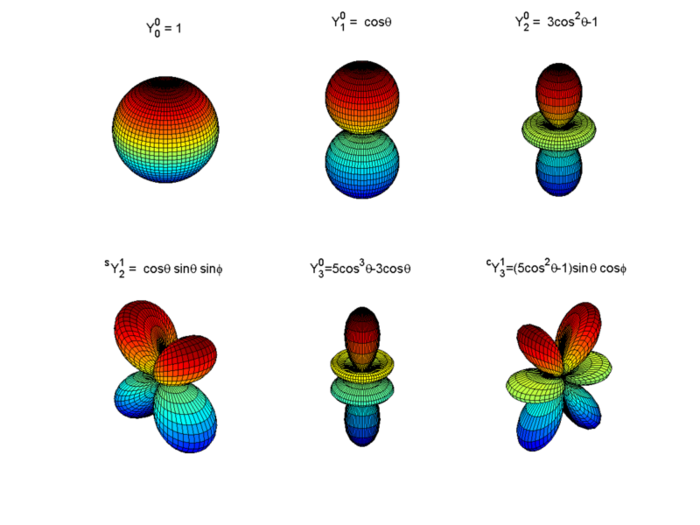
\includegraphics[width = 0.66\textwidth]{figures/sphericalharmonics.png}
        \caption{Spherical harmonics.}
        \label{fig:SH}
    \end{figure}
    
    \item Dipoles, Quadrupoles:
    \begin{itemize}
        \item A cute way to derive the dipole scaling, we can recognize this as essentially taking the derivative of the field at the dipole, and multiplying by the distance between the two. Hopefully this diagram sketches the proof:
        
        \item We can do the say thing with the dipole field. Another screenshot below: 
        
        \begin{figure}
            \centering
            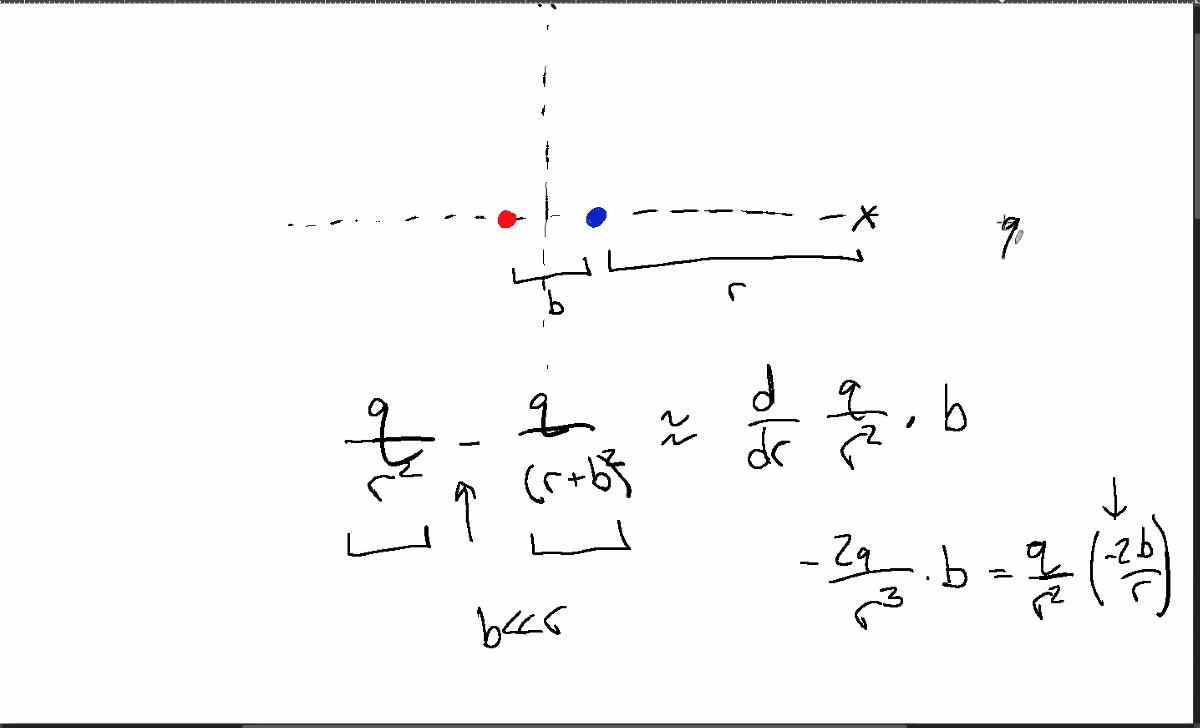
\includegraphics[width=0.75\textwidth]{figures/Screen Shot 2020-09-15 at 12.18.39 PM.png}
            \caption{Dipole}
            \label{fig:dip}
        \end{figure}
        
        \begin{figure}
            \centering
            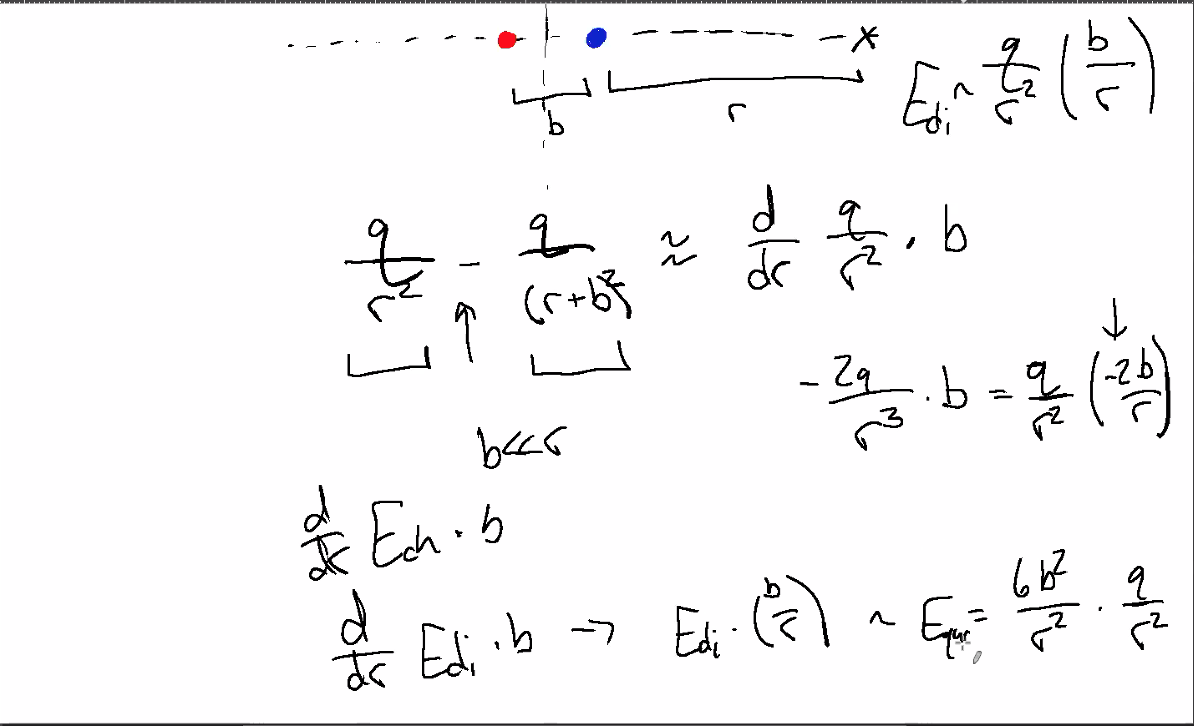
\includegraphics[width=0.75\textwidth]{figures/Screen Shot 2020-09-15 at 12.20.14 PM.png}
            \caption{Quadrupole}
            \label{fig:quad}
        \end{figure}
    \end{itemize}
    
    \item What happens as you spin the dipole? 
    \begin{itemize}
        \item Electric fields move at the speed of light. If $\omega r > c$, you have a problem. You therefore have a distance beyond which the field lines separate. You should be able to get this from the Larmor equation.
        
        \begin{figure}
            \centering
            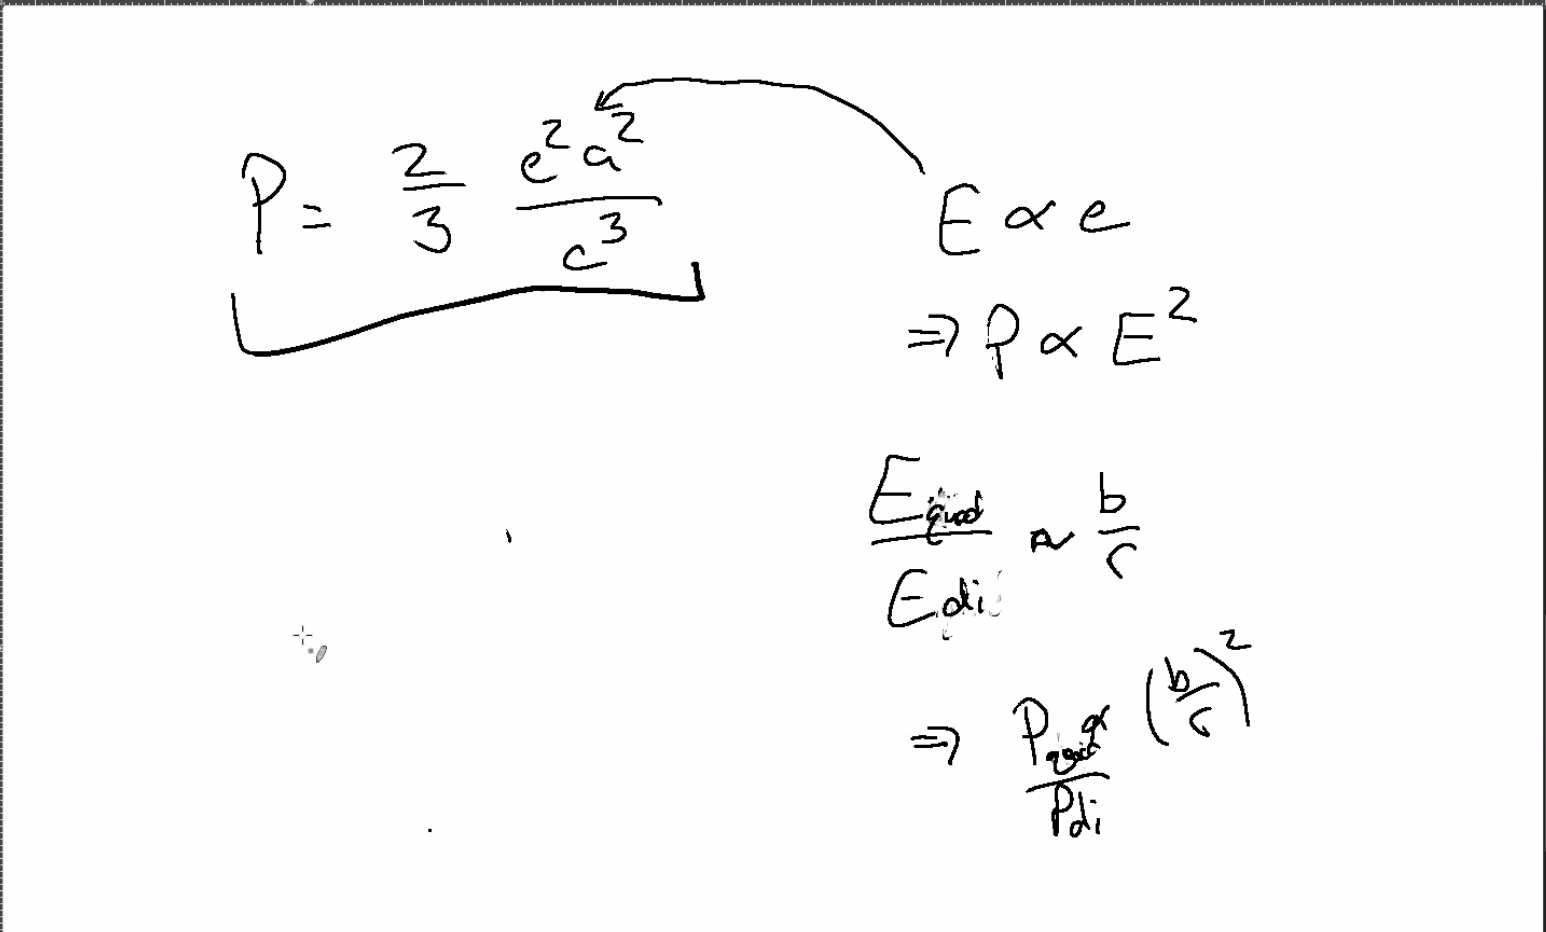
\includegraphics[width=0.66\textwidth]{figures/Screen Shot 2020-09-15 at 12.34.06 PM.png}
            \caption{Power radiated equation.}
            \label{fig:larmorradiate}
        \end{figure}
    \end{itemize}
    
    
\end{itemize}

%%%%%%%%%%%%%%%%%%%%%%%%%%%%%%%%%%%%%%%%%%%%%%%%%%%%%%%%%%%%%%%%%%%%%%%%%%%%%%
%%%%%%%%%%%%%%%%%%%%%%%%%%%%%%%%%%%%%%%%%%%%%%%%%%%%%%%%%%%%%%%%%%%%%%%%%%%%%%
%%%%%%%%%%%%%%%%%%%%%%%%%%%%%%%%%%%%%%%%%%%%%%%%%%%%%%%%%%%%%%%%%%%%%%%%%%%%%%
\newpage
\section{September 17, 2020: Einstein Coefficients \& Radiative Equilibrium}

\subsection{Einstein Coefficients}

\subsubsection{Einstein Coefficients Explained}

These are meant to describe the rates absorbing and re-emitting photons by atoms. By absorbing photons, atoms can store energy in the electronic states. This excited atom will transition back to lower energy, re-emitting that photon with the corresponding energy difference. 

Einstein coefficients are \textbf{macroscopic} approximations of complex, stochastic quantum properties. We can only calculate the true coefficients explicitly for simple cases. \\

\noindent\textbf{Sponenatous Emission}\\

We will first talk about \textbf{spontaneous emission.} Consider two energy levels, $E_1$ and $E_2$. We will have number densities in each of these states $n_i$. The photons that are emitted in this transition have energy $\Delta E$. We universally see a decay law of this spontaneous emission:

\begin{equation}
    n_2 \propto e^{-t/\tau}
\end{equation}

where $\tau$ is specific to the transition. Therefore we define the first Einstein coefficient $A_{21} \equiv 1/\tau$. This has units $\s^{-1}$. If $A_{21}$ is large, it decays faster. Another way to quantify this is the half life which is equal to $\frac{\ln 2}{A_{21}}$. 

We can use the Einstein coefficient in a variety of contexts:

\begin{equation}
    \frac{d n_1}{dt} = n_2 A_{21}
\end{equation}

or

\begin{equation}
    \boxed{\frac{d n_2}{dt} = -n_2 A_{21}}
\end{equation}

It is the boxed equation that gives the exponential behavior that we see universally. \\

\noindent\textbf{Absorption}\\

This sort of looks like the reverse of emission, but it isn't quite. Consider a photon coming in and sending a photon to a higher energy. Should we just invent a new Einstein coefficient? No, because that isn't intrinsic. If we had more photons, we expect that absorption rate to go up:

\begin{equation}
    R \propto I_\nu B_{12}
\end{equation}

The rate here is proportional to the intensity, and $B$ is the absorption coefficient. This takes us from the $1$ energy state to the $2$ energy state. Note that the intensity we plug in $I_\nu$ means the intensity averaged over all directions:

\begin{equation}
    I_\nu = \frac{1}{4\pi} \int \int I_\nu(\hat{s}) d\Omega \phi(\nu) d\nu
\end{equation}

We also need the photon energy to be approximately the energy difference. It doesn't have to be exact (i.e. get the other energy from somewhere else). What governs this width? This is called the \textbf{line profile function} $\phi$ which have units of inverse bandwidth. Basically this $I_\nu$ measures average over all directions of photons that could lead to a transition. We note that the units of $B_{21}$ is:

\begin{equation}
    [B_{12}] = \frac{\hz \cm^2 \sr}{\ergs}
\end{equation}

Also, for convenience, we will define the quantity:

\begin{equation}
    \bar{J} \equiv \frac{1}{4\pi} \int \int I_\nu(\hat{s}) d\Omega \phi(\nu) d\nu
\end{equation}

We therefore have:

\begin{equation}
    \text{Rate} = \bar{J} B_{12}
\end{equation}

We then have:

\begin{equation}
    \frac{d n_2}{dt} = n_1 B_{12} \bar{J}
\end{equation}

and

\begin{equation}
    \frac{d n_1}{dt} = -n_1 B_{12} \bar{J}
\end{equation}

These look almost identical to emission! 

We are saying that $A_{21}$ and $B_{12}$ are intrinsic properties of transitions. If that is true, then they need to work out in all situations including thermal equilibrium. Suppose we are in thermal equilibrium (which isn't necessary for the Einstein coefficients).

We know in thermal equilibrium that Boltzmann statistics give the ratio of number densities in energy states. We also know that rates need to balance in thermodynamic equilibrium. We therefore have:

\begin{equation}
    \frac{n_2}{n_1} = \frac{g_2}{g_1} e^{-\Delta E/kT}
\end{equation}

\begin{equation}
    n_2 A_{21} = n_1 \bar{J} B_{12}
\end{equation}

Now suppose we are in ``local'' thermodynamic equilibrium. This means that radiation is also in equilibrium with ratio of states. We therefore know:

\begin{equation}
    \bar{J} = B_\nu = \frac{2 h \nu^3}{c^2} \frac{1}{e^{h\nu/ kT} - 1}
\end{equation}

Putting these all together, we have:

\begin{equation}
    \frac{g_2}{g_1} \frac{A_{21}}{B_{12}} e^{- \Delta E/kT} = B_\nu
\end{equation}

If you say $h\nu = \Delta E$, we have pretty much the same thing on the right and left, aside from the $-1$ from Boson statistics. However, there is no way that the ratio of $A_{21}/B_{12}$ cannot be intrinsic that \textbf{also} gives the $-1$ from Bosonian statistics. A normal person would say that we made an error on our assumptions, but Einstein said that, even if the functional forms were not compatible, there could be an equivalence \textit{if} there is a $B_{21}$. As it turns out, he was correct, and $B_{21}$ is stimulated emission!\\

\noindent\textbf{Stimulated Emission}\\

This is the true opposite to absorption. But what is it? Here, we have an electron in an excited state, a photon comes by, and the presence of that photon helps the atom transition to the de-excited state. We now have two almost-identical photons. Also, how the heck does that even happen? We can think of the different states of an electron as ``resonances,'' and if a photon comes by with the same standing-wave resonance, it could jiggle it out to a different resonance state. Mathematically, it looks identical to absorption.

\begin{equation}
    \text{Rate} = \bar{J} B_{21} 
\end{equation}

where here $B_{21}$ goes from $2$ to $1$. We also can update our rate equation:

\begin{equation}
    \boxed{n_2 A_{21} = n_1 \bar{J} B_{12} - n_2 \bar{J} B_{21}}
\end{equation}

We can now do what we did before. In LTE, we can manipulate the rate equation to be:

\begin{equation}
    \bar{J} = \frac{A_{21}}{\frac{n_1}{n_2} B_{12} - B_{21}}
\end{equation}

We then use Boltzmann, and get relations for intrinsic properties. \\

\textbf{If the follow equations are true...}

\begin{equation}
    g_1 B_{12} = g_2 B_{21}
\end{equation}

and

\begin{equation}
    A_{21} = \frac{2 h \nu^3}{c^2} B_{21}
\end{equation}

\textbf{then...}

\begin{equation}
    \frac{A_{21}/B_{12}}{\frac{g_1}{g_2} e^{\Delta E/kT} - \frac{B_{21}}{B_{12}}} = \frac{2 h \nu^3}{c^2} \frac{1}{e^{h\nu/kT} - 1}
\end{equation}

\textbf{is true in local thermodynamic equilibrium}. A consequence is that the only number you need to know is the $A_{21}$ coefficient to know all about transitions in an atom. \\

\textbf{Having a large $A_{21}$ means high $B_{21}$ and $B_{12}$ (easily absorb and emit), and you also decay faster spontaneously. } ($A_{21}$ is like an inherent strength since it is the only number that matters). ) Also note, you might see ``oscillator strength'' as a measure of strength:

\begin{equation}
    A_{21} = \frac{2 \pi e^2 }{\lambda^2 c} \frac{g_1}{g_2} \times \underbrace{f_{12}}_{\text{oscillator strength}}
\end{equation}

\subsubsection{LASER: Stimulated Emission}

We start with Einstein (1917) \textit{On the Quantum Theory of Radiation}. Einstein was studying how light interacts with matter. Einstein considered populations of two energy states, if we shine light on a gas, the absorption rate can be given by:

\begin{equation}
    \text{Rate} = n_1 B_{12} n_1 \bar{J}
\end{equation}

He then said excited gases can release photons, given by:

\begin{equation}
    \text{Rate} = n_2 A_{21}
\end{equation}

He then said there can be a third process called stimulated emission. This means that, subject to a stream of photons on an already-excited gas, photons will induce the higher energy electrons to drop levels. This emits more radiation, and this is the basis for lasers! The outgoing photons are all coherent (in-phase). 

\begin{equation}
    \text{Rate} = n_2 B_{21} \bar{J}
\end{equation}

We thus have a balance:

\begin{equation}
    n_1 B_{12} n_1 \bar{J} = n_2 A_{21} +  n_2 B_{21} \bar{J}
\end{equation}

Rearranging this, we get $n_2>n_1$ in order to have emission dominate the process. This is called a population inversion, and is the true basis for lasers. The hard part is achieving population inversions. 


\subsubsection{Einstein Coefficients (Bucknell)}

Here, we get into details on gain media in lasers. Generally, when we talk about photons, we think about an energy density of photons: $\rho(\nu) \partial \nu$. Here, we assume we can take out $\partial \nu$. We can therefore just think of an abstract energy density of photons in a volume. We can a unit square with rectangular length $d=c/n$. We want to calculate the intensity per unit area at the end of the cavity (square wall). The number of photons per second will give us the intensity. We can then calculate the energy density:

\begin{equation}
    I_\nu = N_p \frac{c}{n}
\end{equation}

\begin{equation}
    N_p = \frac{\rho(\nu)\partial \nu}{h \nu}
\end{equation}

This is the intensity of light at a given frequency. So what did Einstein do? The two sections above are just the rest of these videos. Not worth typing it out.

\subsection{Detailed Notes, from Aaron Parsons}

Einstein coefficients describe the absorption and emission of photons via electronic transitions in atoms.  
Suppose we have an atom with 2 energy levels with an energy difference of $\Delta E=h\nu_0$.  Einstein coefficients describe the 
transition rates caused by the interaction of radiation with these discrete energy
levels. There are three coefficients:

\begin{figure}\centering
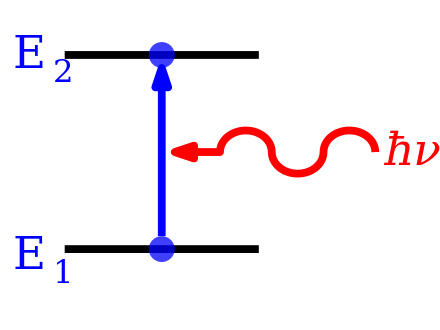
\includegraphics[width=1in]{figures/B12.png}
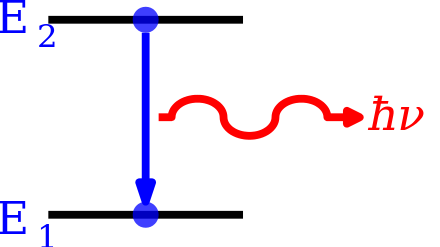
\includegraphics[width=1in]{figures/A21.png}
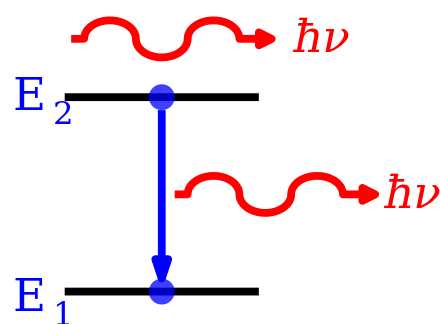
\includegraphics[width=1in]{figures/B21.png}
\caption{Left: Photon absorption rates are described by $B_{12}$.  Center: Spontaneous photon emission rates are described by $\ato$.  Right: Stimulated photon emission rates are described by $B_{21}$.}
\end{figure}

\subsubsection{Spontaneous Emission}

$\ato$ governs decay from energy state 2 to 1.  It is the transition 
probability per unit time for an atom, and has units of $s^{-1}$.  More specifically, the probability an atom
undergoes spontaneous de-excitation and releases a photon is Poisson-distributed, with mean rate
$\ato$. So $\ato^{-1}$ is the mean lifetime of the excited state.   As an example,
$H_\alpha$ ($3\to2$ transition in hydrogen) has an Einstein A coefficient of $\ato\approx 10^9 s^{-1}$.

If $n_2$ describes the number density of atoms in the upper energy state, then the transition rate per volume is given by:
\begin{equation}
r_{\rm spon}=n_2\ato
\end{equation}

\subsubsection{Spontaneous Absorption}

$\bot$ governs photon absorption that causes a transition from the lower to upper energy state ($1\to2$).  In contrast
to the $\ato$ case, absorption requires the presence of photons, so translating $\bot$ to an excitation rate requires
some knowledge of the background radiation field.

To describe the background radiation field, we define the spherically averaged specific intensity:
\begin{equation}
J_\nu \equiv \frac1{4\pi}\int{I_\nu d\Omega}
\end{equation}
We use $J_\nu$ instead of $I_\nu$ (the intensity) because atomic absorption does not depend on direction.
However, we have to remember that there are uncertainties in the energy-level
separations, which means that atoms absorb photons that are not perfectly tuned to
the energy difference between electronic states.  To incorporate this, we use the line profile function, $\phi(\nu)$.  It 
describes
the relative absorption probability around $\nu_0$ (the
absorption frequency), and is subject to the requirement that:
$\int_0^\infty{\phi(\nu)d\nu}=1$.  We can approximate the width of $\phi(\nu)$ as an effective width $\Delta\nu$.
$\Delta\nu$ is affected by many factors:
\begin{itemize}
\item $\ato$ (the natural, uncertainty-based broadening of at atom in isolation),
\item $\nu_0 v_{\rm therm}/c$ (Doppler broadening from thermal motion), and 
\item $n_{coll}\sigma_{coll}v_{rel}$
(collisional broadening, a.k.a. pressure broadening). 
\end{itemize}
Line profile functions are of special interest for studying line emission/absorption, and is discussed later in more detail (see Line Profile Functions).

Using the line profile function, we get the transition probability per unit time associated with spontaneous absorption:
\begin{equation}
t_{ex}^{-1}=\bot\int_0^\infty{J_\nu\phi(\nu)d\nu}\approx\bot\Jbar
\end{equation}

\subsubsection{Stimulated Emission}

$\bto$ governs stimulated emission.  In this example, we are in energy
state 2, and an incoming photon causes a transition to energy level 1 and the
emission of 2 photons.  The transition per unit time is $\bto\Jbar$. For an important case of stimulated emission, see Masers.

\subsubsection{ Einstein Relations among coefficients}

Assume we have many atoms with 2 energy states, and $n_1$ is the \# density
in state 1, ditto for $n_2$.  Assume we are in thermal, steady-state 
equilibrium, so:
$$n_1\bot\Jbar=n_2\ato+n_2\bto\Jbar$$
This is because as many atoms need to be
going from energy state 1 to 2 as visa versa.
A second relation is:
$\Jbar = \frac{n_2\ato}{n_1\bot-n_2\bto}$.
Using the Boltzmann distribution, $\frac{n_2}{n_1}=\frac{g_2}{ g_1}\eboltz$:
$$\Jbar=\frac{{{\frac{\ato}{\bto}}}}{{{{\frac{g_1\bot}{ g_2\bto}}}\eboltzplus-1}}$$

In thermal equilibrium $J_\nu$ is given by the 
$$\begin{aligned}\Jbar&\equiv\int_0^\infty{J_\nu\phi(\nu)d\nu}\\ 
&=\int_0^\infty{B_\nu\phi(\nu)d\nu}\\ 
&\approx B_\nu(\nu_0)\\ 
&=\frac{2h\nu_0^3}{c^2(\eboltzplus-1)}\\ \end{aligned}$$

Combining this with $\Jbar$ earlier, we get:
$$\boxed{g_1\bot=g_2\bto}$$
\centerline{and}
$$\frac{\ato}{\bto}=\frac{2h\nu^3}{ c^2}$$

\subsubsection{ Rewriting source function terms in terms of Einstein coeffs}

In a small volume $dV$:
$$\begin{aligned}j_\nu&\equiv\frac{dE}{ dt\,dV\,d\nu\,d\Omega}\\ 
&=\frac{h\nu_0\ato n_2\phi(\nu)}{4\pi}\\ \end{aligned}$$

We can express the extinction coefficient, $\alpha_\nu$, in terms of the Einstein coefficients.  The
excitation probability per time is $n_1B_{12}\Jbar$, and
the energy lost in crossing the small volume 
$\propto n_1\bot\frac{I_\nu d\Omega}{4\pi}\phi(\nu)d\nu$
(it is the probability per time per volume of going $1\to2$ by absorbing 
$I_\nu$ from
a cone of solid angle $d\Omega$ and frequency range $[\nu,\nu+d\nu]$). Thus,
the energy is given by:
$$\begin{aligned}E&=n_1\bot\frac{I_\nu d\Omega}{4\pi}\phi(\nu)d\nu h\nu dt\,dV\\ 
&=\alpha_\nu I_\nu ds\,dt\,d\Omega\,dA\,d\nu\\ \end{aligned}$$ 
Recognizing that $dV=dA\,ds$:
$$\alpha_\nu=\frac{n_1\bot\phi(\nu)}{4\pi}h\nu$$
Correcting for stimulated emission, we get:
$$\boxed{\alpha_\nu=\frac{(n_1\bot-n_2\bto)\phi(\nu)h\nu}{4\pi}}$$

\subsubsection{ Estimating Cross-Sections }

The absorption coefficient, written in terms of Einstein constants is:
$$\alpha_\nu=\frac{n_1\bot\phi(\nu)}{4\pi}h\nu=n_1\sigot$$
Thus, the cross section of an atom for absorption of a photon is:
$$\sigot=\frac{\bot\phi(\nu)h\nu}{4\pi}$$
To estimate $\bot$, we use the fact that, ignoring $g$'s, $\bot\sim\bto$,
and $\frac{\ato}{\bto}=\frac{2h\nu^3}{ c^2}$.  Then using the approximation that
that $\phi(\nu)\sim\inv{\Delta\nu}$, we get:
$$\sigot\sim\frac{\ato}{\left(\frac{2h\nu^3}{ c^2}\right)}
\frac{h\nu}{4\pi\Delta\nu}$$
$$\boxed{\sigot\sim\frac{\lambda^2}{8\pi}\frac{\ato}{\Delta\nu}}$$
In a single atom, $\Delta\nu\sim\ato$, so $\sigot\sim\frac{\lambda^2}{8\pi}$.


\subsubsection{Einstein coefficients: a closer look}
\textit{Why} do we get spontaneous decay and stimulated emission? Quantum mechanics has the answer -- see below (warning: all of the following is done in SI units).

These processes can be understood using a bit of quantum mechanics. To do so, let's consider a system with two energy eigenstates, $\psi_a$ and $\psi_b$. In general, the particle will be in some linear combination of $\psi_a$ and $\psi_b$:
\begin{equation}
\Psi = c_a\psi_a + c_b\psi_b
\end{equation}
The probabilities are $|c_a|^2$ and $|c_b|^2$, and they of course must sum to unity at all times.

Now, let's suppose the electron starts off in $\psi_a$ at $t=0$, so that $c_a(t=0) = 1$ and $c_b(t=0) = 0$. To first-order, time \textit{dependent} perturbation theory tells us:
\begin{equation}
c_b \approx \frac{-i}{\hbar}\int_0^t H_{ba}e^{i\omega_0t'}dt',
\end{equation}
where $H'_{ba} \equiv \langle \psi_a | \hat{H'} | \psi_b \rangle$ is the off diagonal component of the perturbing Hamiltonian $\hat{H'}$ and $\omega_0 \equiv (E_b - E_a)/\hbar > 0$. The derivation of this result is too detailed to reproduce here, but can be found in any quantum mechanics textbook. Note that even though the system started off entirely in $\psi_a$, the introduction of a perturbation means that the probabilities can change as a function of a time -- eventually, it may be that $c_b(t) = 1$ and the particle is entirely in $\psi_b$. \textit{This is exactly what a quantum transition is!}

Now, let's consider what happens when our perturbation is modulated by a sinusoidal time dependence -- say, an electric field polarized in the $z$ direction:
\begin{equation}
\hat{H'} = V(x,y,z)\cos(\omega t) = -qE_0z\cos(\omega t)
\end{equation}
Then: 
\begin{equation}
H_{ba} = -\alpha E_0 \cos(\omega t), 
\end{equation}
where we will now use:
\begin{equation}
\alpha \equiv q \langle \psi_b | z | \psi_a \rangle.
\end{equation}

Plugging into our expression from perturbation theory and integrating we get:
\begin{equation}
c_b(t) = \frac{-\alpha E_0}{2\hbar}\left[\frac{e^{i(\omega_0 + \omega)t} -1}{\omega_0 + \omega}  + \frac{e^{i(\omega_0 - \omega)t} -1}{\omega_0 - \omega}\right].
\end{equation}
Let's now consider only perturbations oscillating at near the transition frequency -- i.e., $\omega_0 \approx \omega$. This is a reasonable thing to do since driving frequencies far from $\omega_0$ contribute negligibly to the above expression. Then we end up with:
\begin{equation}
c_b(t) = \frac{i\alpha E_0}{\hbar}\frac{\sin\left(\frac{(\omega_0 - \omega)t}{2}\right)}{\omega_0 - \omega}e^{i(\omega_0-\omega)t/2}.
\end{equation}
The probability that the particle has ``transitioned'' from its initial state $\psi_a$ to the other state $\psi_b$ is just given by $|c_b|^2$:
\begin{equation}
P_{a \rightarrow b}(t) = \frac{|\alpha E_0|^2}{\hbar^2}\frac{\sin^2\left(\frac{(\omega_0 - \omega)t}{2}\right)}{(\omega_0 - \omega)^2}.
\end{equation}
But nothing in this derivation relied on the fact that the particle started off in the lower energy state! Therefore, we must conclude that:
\begin{equation}
P_{a \rightarrow b}(t)  = P_{b \rightarrow a}(t). 
\end{equation}
Wow! These equations are full of interesting physics. They tell us that if a particle starts off in a higher energy state, and then we shine light on it then, because the light is just an oscillating electric (and magnetic) field, the resulting perturbation to the Hamiltonian can induce the particle to fall down to the lower energy state. This is exactly the phenomenon of stimulated emission. Note also that shining light on the particle can \textit{also} cause it to jump \textit{up} an energy state -- and the probabilities of going from the lower to the upper state and from the upper to the lower state are the same! This is the reason the Einstein coefficients $B_{21}$ and $B_{12}$ are the same (up to degeneracy, but that's a different story).

What about spontaneous decay to a lower energy state? In quantum electrodynamics, there's no such thing as a nonzero electric field -- even if you're not shining a light, the "ground state" still has a nonzero field. And it's this field that acts as the perturbation. So, "spontaneous" decay is really not spontaneous -- it's just stimulated decay by a different electric field!


So far we've considered the impact of a single plane wave polarized in the $z$ direction. In reality of course, things are a little messier. Suppose we shine light of a whole bunch of frequencies, with $\rho(\omega)$ representing the energy density in some $d\omega$. Then, the transition probability can be expressed as:
\begin{equation}
P_{\rm transition}(t) = \frac{2|\alpha|^2}{\epsilon_0\hbar^2}\int_0^{\infty} \rho(\omega) \frac{\sin^2\left(\frac{(\omega_0 - \omega)t}{2}\right)}{(\omega_0 - \omega)^2} d\omega \approx \frac{\pi|\alpha|^2}{\epsilon_0\hbar^2}\rho(\omega_0)t
\end{equation}
We'll make one more correction, which is that we want to account for light coming in at all angles and polarizations. Therefore, we'll just generalize:
\begin{equation}
\vec{\alpha} = q\langle \psi_b | \vec{r} | \psi_a \rangle,
\end{equation}
and tack on a factor of 1/3 to $P_{\rm transition}$ in averaging over all polarizations and directions. Then the transition probability becomes:
\begin{equation}
P_{\rm transition}(t) = \frac{\pi|\vec{\alpha}|^2}{3\epsilon_0\hbar^2}\rho(\omega_0)t.
\end{equation}

Finally, we can get our Einstein coefficients; for brevity, and since part of this is already covered in the video, I'll skip a couple steps. If we demand statistical and thermal equilibrium
\begin{equation}
\rho(\omega_0) = \frac{A}{\exp[\hbar\omega_0/k_BT]B_{ab}-B_{ba}} = \frac{\hbar}{\pi^2c^3}\frac{\omega^3}{\exp[\hbar\omega_0/k_BT]-1}
\end{equation}
Note that I've dropped the degeneracy factors here, for simplicity, but they can be easily put back in. Comparing the two expression implies that:
\begin{equation}
A = \frac{\omega^3_0 |\vec{\alpha}|^2}{3\pi\epsilon_0\hbar c^3}.
\end{equation}
And there we have it! The above expression allows us to calculate $A$ directly! The only thing you really need to calculate is $\vec{\alpha} = \langle \psi_b | \vec{r} | \psi_a \rangle$. For most atoms, this is a bit complicated, since it requires you to know the wavefunctions. But for hydrogen, this is completely doable -- you can look up the wavefunctions of hydrogen (or solve the Schrodinger equation yourself, if you like...). Note that for a spherically symmetric Hamiltonian, the elements of $\vec{\alpha}$ often go to zero, so this really isn't too bad. If you prefer not to calculate the Einstein coefficient directly, then see \textit{Estimating Atomic Transition Strengths} for a quick and dirty way.

\subsection{Radiative Equilibrium}

Radiative equilibrium is the idea of achieving thermal equilibrium just through radiative. We start with radiative transfer:

\begin{equation}
    \dfrac{dI_\nu}{ds} = j_\nu - \alpha_\nu I_\nu
\end{equation}

However, this ignores a temporal component. Considering some intensity of light hitting a cloud, heating the cloud. As a consequence, the emissivity increase. We can then add a new term to our radiative transfer equation:

\begin{equation}
    \boxed{\frac{1}{c}\dfrac{dI_\nu}{ds} + \frac{\partial I_\nu}{\partial s} = j_\nu - \alpha_\nu I_\nu}
\end{equation}

Remember we defined a source function that asymptotes to the Planck function in local therodynamic equilibrium. Remember, though, that the flux $F = \int B_\nu d\nu d \Omega = \sigma T^4$. This flux is the energy per time per surface area. We should compare this at equilibrium to the energy flowing \textit{in} since we are in equilibria. How do we evaluate energy coming in?

We can account for this by considering the directionality of the sources. Imagine a cloud being heated from multiple sides. We care about all the energy flowing in which is heating the cloud. Here, we define:

\begin{equation}
    J_\nu \equiv \frac{1}{4\pi}\int I_\nu d\Omega
\end{equation}

which can be thought of as a mean intensity -- the average coming in from all directions onto an object like a cloud. We then can integrate this over bandwidth which would give us an accurate comparison of energy out versus energy in. Our flux in is thus $4\pi J_\nu = 4\pi J$. Our flux in is just $\sigma T^4$. One thing we want to mention is that $\alpha_\nu$ is still frequency dependent. To say this clearly, imagine where we have a blackbody spectrum, but a backgorund source doesn't have to be Planckian. However, $\alpha_\nu$ is different for the two places as well. So we should be talking about an average $\alpha_\nu$ as well. We can therefore define this:

\begin{equation}
    \alpha_J \equiv \frac{\int \alpha_\nu J_\nu d\nu}{J}
\end{equation}

We can then compare this to $\alpha_B$ which is the same for a blackbody spectrum. We then need to compare:

\begin{equation}
    \boxed{\alpha_J \pi J = \alpha_B \sigma T^4}
\end{equation}

We thus have, in radiative equilibrium (with background light tied up in the $J$ factor), the temperature of a gas is given by:

\begin{equation}
    \boxed{T = \left(\frac{\alpha_J}{\alpha_B} \frac{\pi}{\sigma} J\right)^{1/4}}
\end{equation}

If we are not in equilibrium, we can estimate the time scale for heating by comparing the energy per unit volume required to heat a gas with temperature $T$ to the power per volume flowing in from radiation:

\begin{equation}
    \boxed{t_{heat} \sim \frac{\frac{3}{2} n k T}{4\pi \alpha_J J}}
\end{equation}

Likewise, the cooling timescale can be found:

\begin{equation}
    \boxed{t_{cool} \sim \frac{\frac{3}{2} n k T}{\alpha_B \sigma T^4}}
\end{equation}

\subsection{Detailed Notes, from Aaron Parsons:}

\subsubsection{ Local Thermodynamic Equilibrium (LTE)}

Local Thermodynamic Equilibrium means 
$$S_\nu=B_\nu(T)$$
where $T$ is {\it local}.
Take a sphere at surface temp $T$, with some gas (matter) inside it.   Allow
to come to thermal equilibrium.  Inside the sphere, 
you see a Planckian spectrum ($I_\nu = B_\nu$).  Now suppose you take a box of
gas (it is both emissive and absorbent) and shoot rays of photons through
that box. According to the Radiative Transfer Equation, these photons suffer some absorption: 
$$dI_\nu = -\alpha _\nu ds I_\nu$$
But
those photons also pick up some intensity: 
$$dI_\nu = +j_\nu ds$$
But since the photons
should not pick up energy going through the box (everything is at the same
temperature), 
$$S_\nu\equiv\frac{j_\nu}{\alpha_\nu}=I_\nu=B_\nu$$

Now suppose you let all the photons out of this sphere.  Those photons will
no longer be in thermal equilibrium with the gas.  Suppose we magically fix
the temperature of the gas at this point.  The source function will remain the
same (it will still be the case that $S_\nu = B_\nu$) because the source 
function {\it is a property of the matter alone} (the absorptive and emissive 
properties of it).  However, $I_\nu\ne B_\nu$.\par

Suppose we look along a column of this gas.  At each point, the source
function will be: $S_\nu=B_\nu(T)$.  Therefore, $I_\nu$ along that column
will be: 
\def\np{{\nu^\prime}}
$$I_\nu=\int_0^{T_\nu}{S_\nu(T_\np)e^{-(T_\np-T_\nu)}dT_\np}$$


\subsubsection{ Radiative Equilibrium and Relations among Einstein Coefficients}

Assume we have many atoms with 2 energy states, and $n_1$ is the \# density
in state 1, ditto for $n_2$.  Assume we are in thermal, steady-state 
equilibrium, so:
$$n_1\bot\Jbar=n_2\ato+n_2\bto\Jbar$$
This is because as many atoms need to be
going from energy state 1 to 2 as visa versa.
A second relation is:
$\Jbar = \frac{n_2\ato}{ n_1\bot-n_2\bto}$.
Using the Boltzmann distribution, $\frac{n_2}{ n_1}=\frac{g_2}{ g_1}\eboltz$:
$$\Jbar=\frac{\frac{\ato}{\bto}}{\frac{g_1\bot}{ g_2\bto}\eboltz-1}$$

In thermal equilibrium $J_\nu$ is given by the:
$$\begin{aligned}\Jbar&\equiv\int_0^\infty{J_\nu\phi(\nu)d\nu}\\ 
&=\int_0^\infty{B_\nu\phi(\nu)d\nu}\\ 
&\approx B_\nu(\nu_0)\\ 
&=\frac{2h\nu_0^3}{ c^2(\eboltz-1)}\\ \end{aligned}$$

Combining this with $\Jbar$ earlier, we get:
$$\boxed{g_1\bot=g_2\bto}$$
\centerline{and}
$$\frac{\ato}{\bto}=\frac{2h\nu^3}{c^2}$$

\subsection{Class Notes}

This is one of the touchstones of the class, and there \textbf{will absolutely be a prelim question on this topic}. They connect the microscopic to the macroscropic. In a very real way, Einstein Coefficients turn molecules and atoms into light. We should know the $\lya$ value of the $A$ coefficient. 

\textbf{Are the Einstein coefficients connected only when we have LTE?}

No! $A_{21}$, and the others, are intrinsic to the atom. They do not change whether or not we are in equilibrium. They are determined by the physics of the molecule and the transition only. In deriving them, we only assumed LTE for a calibration point. 

\par\noindent\rule{\textwidth}{0.4pt}

Using the terminology introduced in the discussion of Radiative Equilibrium (e.g. $\alpha_J$,
$\alpha_B$, $J$, $T$), estimate fractionally how much hotter you'd expect a piece of aluminum in space (where
it is thermally isolated) to be relative to the same piece painted white.

Well, the temperature scales like:

\begin{equation}
    \boxed{T = \left(\frac{\alpha_J}{\alpha_B} \frac{\pi}{\sigma} J\right)^{1/4}}
\end{equation}

Here, we are preferentially rejecting light, and letting light inside (infrared being re-radiated) out. This is equivalent to the atmosphere problem, but almost in reverse. $\alpha_B$ does not change, neither does surface area or constants. However, $J$ in the above equation, does change! So how white is ``white'' and how ``white'' is aluminum?

We then need to estimate $\alpha_J$ for white and for aluminum. Reasonable estimate gives the ratio of $2$ or so?

\par\noindent\rule{\textwidth}{0.4pt}
\textbf{Is it clear?}

$A_{21}$ for the 21cm hyperfine transition of H is about $3\cdot 10^{-15}$ s$^{-1}$.  The 
frequency width of this transition is often set by the thermal motion of gas. Assuming
$\Delta\nu\approx \nu_0 v/c$, where $\frac12 mv^2=kT$, we get $\Delta\nu\approx1$ kHz.
If a 
HI cloud in our galaxy has a temperature of 100 K and about 10 hydrogen atoms per
cubic cm, how big does it need to be to be optically thick in 21 cm?  (Many such such clouds
*are* optically thick, so think carefully...).  How many such clouds do you think are
in the Milky Way?\\

In this problem, we want to solve for $s$. We need to estimate $\sigma$ since $\tau = n \sigma s$. We can estimate $A_{21}$ coefficients only with a $\sigma$. One way to approach this is with dimensions:

We know $A_{21}$ makes photons, so we should be able to make an emissivity $j_\nu$ from the coefficient. $j_\nu$ has units of specific intensity per length. Let's cook something up with each term:

\begin{equation}
    j_\nu = \underbrace{h\nu}_{\text{energy}} \underbrace{A_{21}}_{\text{rate}} \underbrace{\frac{1}{4\pi}}_{\text{isotropic}} \underbrace{n}_{\text{number density}} \underbrace{\phi(\nu)}_{\text{line profile}}
\end{equation}

Also, $\phi(\nu) = \frac{1}{\Delta \nu}$. We can get this by $mv^2 \sim kT \rightarrow \Delta \nu = \frac{v}{c}\nu_0$

Also, we know that $\alpha_\nu I_\nu$ has the same units, so we have do a similar thing:

\begin{equation}
    \alpha_\nu I_\nu = \underbrace{h\nu}_{\text{energy}} \underbrace{B_{21}}_{\text{rate}}
    \underbrace{\bar{J}}_{\text{for correct units}}\underbrace{\frac{1}{4\pi}}_{\text{isotropic}} \underbrace{n}_{\text{number density}} \underbrace{\phi(\nu)}_{\text{line profile}}
\end{equation}

However, $I_\nu$ and $\bar{J}$ are pretty much the same thing in the above equation, so we can cancel. We then get:

\begin{equation}
    n \sigma = h\nu \frac{1}{4\pi} n_1 B_{12} \phi(\nu)
\end{equation}

We can also sort of cancel the $n$s to approximate a $\sigma$. However, we are doing an approximation here. We need to account for stimulated emission. We want to stress here that stimulated emission is NOT emissivity. It is the time-reverse of absorption. We therefore have (\textbf{if stimulated emission is not important}):

\begin{equation}
    \sigma \approx \frac{h \nu}{4\pi} \frac{g_2}{g_1} \left(\frac{2h\nu^3}{c^2}\right)^{-1} A_{21} \phi(\nu)
\end{equation}

\begin{equation}
    \boxed{\sigma \approx \frac{A_{21}}{4\pi} \frac{\lambda^2}{\Delta \nu}}
\end{equation}

This is true when $\boxed{\text{stimulated emission is not important}}$. How do you know when stimulated emission is important? When atoms are not in the ground state! You need the excited state to be released own. Can we put all our atoms in the excited state? Not really. The closer you are to equilibrium, the more you have to worry about stimulated emission. The calculated effective cross section is $\sigma \sim 1 \times 10^{-14} \cm^2$. This corresponds to a distance of $s = 10^{13} \cm$. This is way smaller than a parsec. This means we could have a million of these clouds stretched end to end. That doesn't seem right -- so is our galaxy in statistical equilibrium? Absolutely. We are so deep into thermal equilibrium. We need to account for stimulated emission, and therefore should not have used this correct approximation. 

Doing the correct calculation should give a few parsecs as the correct answer. 


%%%%%%%%%%%%%%%%%%%%%%%%%%%%%%%%%%%%%%%%%%%%%%%%%%%%%%%%%%%%%%%%%%%%%%%%%%%%%%
%%%%%%%%%%%%%%%%%%%%%%%%%%%%%%%%%%%%%%%%%%%%%%%%%%%%%%%%%%%%%%%%%%%%%%%%%%%%%%
%%%%%%%%%%%%%%%%%%%%%%%%%%%%%%%%%%%%%%%%%%%%%%%%%%%%%%%%%%%%%%%%%%%%%%%%%%%%%%
\newpage
\section{September 22, 2020: Line Profile Functions, Spectral Line Broadening, and Zeeman Splitting}

\subsection{Spectral Line Broadening}

\subsubsection{Line Profile Functions (Spectral Line Broadening)}

\textbf{In one sentence, line profile functions dictate the shape of spectral line emission as a function of frequency. }

Suppose we have an atom with an electron in an excited state that releases a photon and decays. We probably expect $\Delta E = h \nu$. On average, that's true, but there's actually a spread in the dsitribution of photon energies that you get. The center of that distribution corresponds to the energy difference $h \nu$. There's a probability, however, that you get a slightly lower or higher frequency!

The function that describes this probability is called the \textbf{line profile function} $\phi(\nu)$. What is the origin of this spread away from the center?

\begin{itemize}
    \item \textbf{Natural (Intrinsic) Broadening}
    \begin{itemize}
        \item This is the most difficult to understand. 
        \item Consider a collection of aotms in an excited state. Then you measure how many photons come off as a function of time, ignoring stimulated emission and the like. We find an exponential fall off over time $(\propto e^{-\tau}$. This probabilistic decay is interesting -- it tells us about the stability and the shape of the line profile function. 
        \item Why? Any profile in time has a profile in frequency. Taking a FT of the exponential decay gives a feature with an envelop. A shallow decay leads to a narrow peak; a sharp decay is a wide peak.
        \item Previously, we have talked of $A_{10}$. This relates to decays, so we must be able to relate $\tau$ to $A_{10}$ by $\tau \sim A_{10} t$. A large $A_{10}$ gives steeper decays! It turns out that:
        
        \begin{equation}
            \boxed{\phi(\nu) = \frac{A_{10}}{4\pi^2} \frac{1}{\left(\nu - \nu_0\right)^2 + \left(\frac{A_{10}}{4\pi}\right)^2}}
        \end{equation}
        
        \item This is the general form for an exponential decay controlled by an Einstein $A$ coefficient. This is the natural line width arising from the Einstein $A$. This is called a \textbf{Lorentzian} profile. This is a measure of how easy it is to excite or de-excite this transition!
    \end{itemize}
    \item \textbf{Doppler Broadening}
    \begin{itemize}
        \item Easier to understand. Consider observing a bunch of atoms emitting photons and moving in different directions. As a result, the photons are moving in our rest frame and therefore there is slight Doppler Shift. Even if the natural line profile is thin, the distribution of photons will reflect the underlying distribution of velocities of these atoms. 
        \item A bunch of atoms in thermal equilibrium lets us estimate a $v_{rms}$ for this collection of atoms. This gives us:
        
        \begin{equation}
            v_{rms}^2 = \frac{2kT}{m}
        \end{equation}
        
        \item Therefore the \textbf{Doppler Width} is given by:
        
        \begin{equation}
            \boxed{\Delta \nu_0 = \frac{\nu_0}{c} v_{rms}}
        \end{equation}
        
        We can also work out, given a Maxwellian distribution, what the line profile function is:
        
        \begin{equation}
            \boxed{\phi(\nu) = \frac{1}{\Delta \nu_0 \sqrt{\pi}} e^{-\frac{\left(\nu-\nu_0\right)^2}{\Delta \nu_0^2}}}
        \end{equation}
        
        \item This is a Gaussian! Another consequence is that higher temperatures mean wider frequencies.
        
        \item One thing to note is that \textbf{bulk flows} are not the same as Doppler Broadening. This will shift the center frequency, but we will still have a distribution.
        
        \item Also, anything that creates differential motion can look like Doppler Broadening. One thing that creates this in astronomy is turbulence! Turbulence can be incorporated into the velocities of Doppler Broadening. 
    \end{itemize}
    
    \item \textbf{A sidenote:}
    \begin{itemize}
        \item It is often necessary to consider both a Lorentzian and a Doppler profile at the same time. This is a Voigt Profile, and is the convolution of a Lorentizan and a Gaussian profile.
        
        \item We need both because one almost never dominates over the other, so we have imprints of both. It takes into account thermal broadening at the center and Lorentzian wings.
    \end{itemize}
    
    \item \textbf{Collisional Broadening}
    
    \begin{itemize}
        \item As you might imagine, you now have a bunch of atoms that are densely packed for frequent collisions. These collisions interfere with natural emission processes. Remember that natural decay process from earlier? Collisions interfere with this by allowing for more frequent collisions (sort of like stimulated emission?). 
        
        \item As a consequence, collisional broadening is wider than Lorentzian.
        
        \item When the timescale of collision is comparable to decay timescales, we get artificially broadened line profile function:
        
        \begin{equation}
            t_{collision} \sim \frac{1}{A_{10}}
        \end{equation}
        
        \item Remember we talked about collision rates? $R = n \sigma v$. For this rate to impact our line profile function, our rate needs to be:
        
        \begin{equation}
            R \sim A_{10}
        \end{equation}
        
        \item This is saying that we need high densities and velocities, also known as high pressure! That is why this is sometimes called pressure broadening.
        
        \item Also, the cross section determines the importance of collisional broadening:
        
        \begin{equation}
            t_{interaction} \propto \sigma^{-1}
        \end{equation}
        
        \item This means that different interactions give different timescales. Coulomb is inverse square, dipole is inverse cube, etc., giving wildly different cross sections for different interactions. 
        
        \item All of this is to say that different shapes of collisional broadening tell us about the mechanism (i.e., the interaction) causing the width. 
        
        
    \end{itemize}
\end{itemize}

\subsubsection{Effects of Line Broadening} 

\subsubsection{More Notes on Line Profile Function}

The line profile function, $\phi(\nu)$, describes the
distribution of absorption/emission around $\nu_0$ (the
center transition frequency), and is subject to the requirement that:
$$\int_0^\infty{\phi(\nu)d\nu}=1$$
Therefore, the line profile function represents the probability of getting a photon around $\nu_0$. 
Say that $\Delta\nu$ is the width
of the distribution around $\nu_0$.  $\Delta \nu $ is affected by three factors:
$\ato$ (the natural, uncertainty-based broadening of at atom in isolation),
$\nu_0 V_T/ c$ (the thermal, Doppler-based broadening), and 
$n_{coll}\sigma_{coll}v_{rel}$
(collisional broadening, a.k.a. pressure broadening).
So really, the transition probability per unit time is:
$$R_{ex}^{-1}=\bot\int_0^\infty{J_\nu\phi(\nu)d\nu}\approx\bot\bar J$$

\textbf{Natural (Lorentzian) Broadening}:\\

Natural (intrinsic) Broadening is one cause of the width $\Delta\nu$ in a line profile function $\phi(\nu)$. This type of spectral line broadening arises from the spontaneous decay rate $A_{10}$. If you have a bunch of atoms, their lifetimes are affected by the uncertainty in their energy states from quantum mechanics (Heisenberg Uncertainty Principle). 

$$\Delta E\Delta t \sim \hbar$$\\

A photon in a certain energy state will therefore have a range of possible frequencies when it decays to a lower state.

$$\Delta \nu \sim {\frac{\Delta E}{h}} \sim {\frac{1}{2\pi \Delta t}}$$\\

The line profile function resulting from Natural Broadening is the Lorentzian Profile. It is proportional to $A_{10}$. That is, larger $A$'s (faster/stronger decays, or a stepper decay profile) result in more broadening (wider profile function).\\

\begin{figure}[ht]
    \centering
    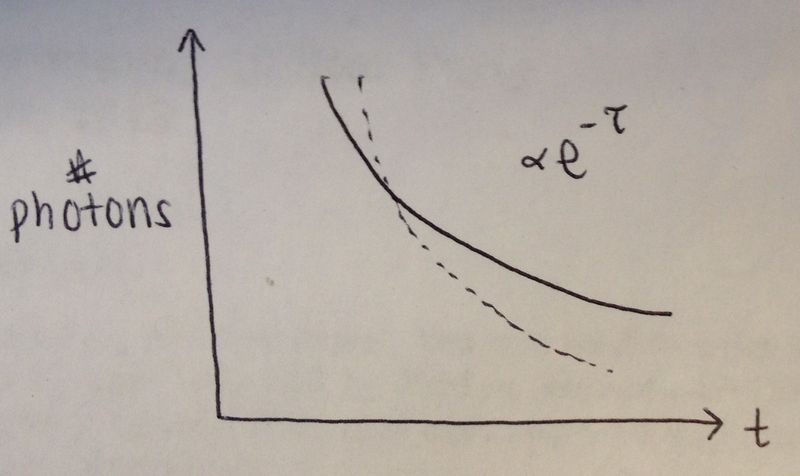
\includegraphics[width=0.66\textwidth]{figures/decay.jpg}
    \caption{Spontaneous decay profile.}
    \label{fig:decay}
\end{figure}

\begin{figure}[ht]
    \centering
    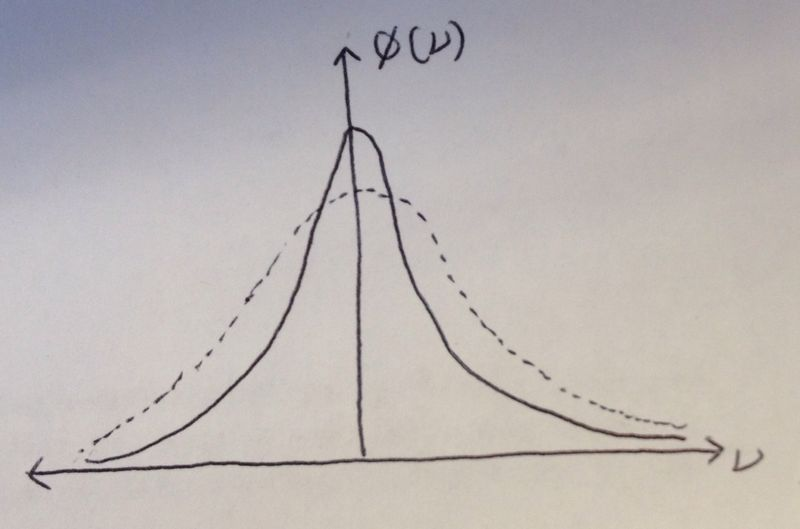
\includegraphics[width=0.66\textwidth]{figures/natural.jpg}
    \caption{Natural broadening line profile.}
    \label{fig:natural}
\end{figure}


$$\phi(\nu) \propto A_{10}$$
$$\phi(\nu) = {\frac{A_{10}}{4\pi^{2}}}{\frac{1}{(\nu-\nu_{0})^{2}+({\frac{A_{10}}{4\pi}})^{2}}}$$

The peak value of the profile occurs when $\nu =\nu_{0}$.

$$\phi_{peak} = {\frac{4}{A_{10}}}$$ \\

This can be used to calculate the FWHM by setting ${\frac{\phi_{peak}}{2}} = \phi(\nu)$ and solving for $2\times (\nu-\nu_{0})$. The result is:

$$\Delta\nu_{FWHM} = {\frac{A_{10}}{2\pi}}$$\\

A typical lifetime for an atomic energy state is $10^{-8}$ seconds, which corresponds to a natural line width of $6.6 \times 10^{-8}$ eV.\\

If radiation is present, then stimulated emission effects must be added to the spontaneous emission ones. Overall though, Natural Line Broadening is not the dominant broadening effect and isn't often directly observed, except in the line wings.

\textbf{Doppler (Gaussian) Broadening}:\\

Doppler Broadening is one cause of the width $\Delta\nu$ in a line profile function $\phi(\nu)$. This type of spectral line broadening arises from the thermal motions of atoms. There will be a velocity distribution for these atoms which causes redshifted and blueshifted photons. Therefore, the Doppler effect leads to variation in the absorbed frequency $\nu$. \\

The Doppler shift is given by: 

$$\nu = \nu_{0}\bigg(1+{\frac{v}{c}}\bigg)$$

where $v$ is the line-of-sight velocity of the absorbing atom. The amplitude of the frequency shift is therefore given by: 

$$\Delta \nu = \nu_{0}{\frac{v}{c}}$$

Recall that the distribution of particle speeds in local thermodynamic equilibrium is Maxwellian:

$${\frac{1}{2}}mv^{2} \sim kT $$
$$v \sim \sqrt{{\frac{2kT}{m}}} $$

Plugging this velocity into the Doppler width gives:

$$\Delta \nu = {\frac{\nu_{0}}{c}}\sqrt{{\frac{2kT}{m}}} $$

The line profile function resulting from Doppler Broadening is a Gaussian Profile. 

$$\phi(\nu) = {\frac{1}{\Delta\nu\sqrt{\pi}}}e^{-{\frac{(\nu-\nu_{0})^{2}}{\Delta\nu^{2}}}} $$ \\

\begin{figure}[ht]
    \centering
    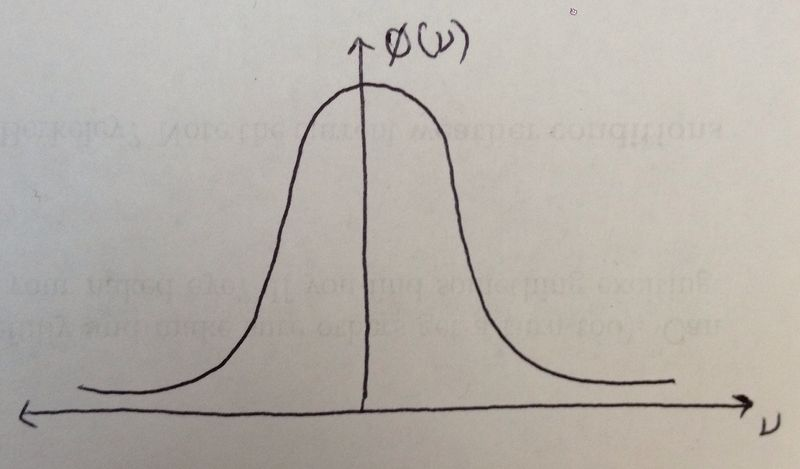
\includegraphics[width=0.66\textwidth]{figures/doppler.jpg}
    \caption{Doppler broadening line profile.}
    \label{fig:dopp}
\end{figure}

The peak value of the profile occurs when $\nu = \nu_{0}$.

$$\phi_{peak} = {\frac{1}{\Delta\nu\sqrt{\pi}}}$$ \\

This can be used to calculate the FWHM by setting ${\frac{\phi_{peak}}{2}} = \phi(\nu)$ and solving for $2\times (\nu-\nu_{0})$. The result is:

$$\Delta\nu_{FWHM} = 1.665\Delta\nu$$ \\

One thing to note is that as temperature increases, there is a greater spread in velocities. However, the number of atoms remains the same, so the peak in the above plot would drop $\bigg($since $\int_{0}^{\infty} \phi(\nu) d\nu = 1\bigg)$. Therefore, it is possible to go from an optically thick medium to optically thin. Up until now the thermal velocity distribution has been used, but turbulence can also cause a spread in velocities. The total Doppler Broadening can be found by adding the two components in quadrature. 

$$v_{total}^{2} = v_{thermal}^{2} + v_{turb}^{2}$$\\

Doppler Broadening as discussed above refers to the differential movement of atoms. There can also be a bulk motion of the atoms in a particular direction, which is a shift in $\nu_{0}$.

\textbf{The Voigt Profile}\\

The Voigt Profile is a convolution of the Lorentzian Profile from Natural Broadening and the Gaussian Profile from Doppler Broadening. It is dominated by the Lorentzian wings and thermal Doppler Broadening in its center. It is a normalized function.

\begin{figure}[ht]
    \centering
    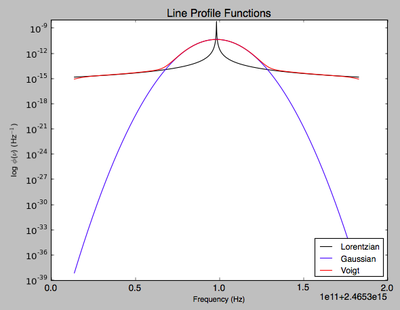
\includegraphics[width=0.66\textwidth]{figures/hw11pic1.png}
    \caption{Voigt profile.}
    \label{fig:voigt1}
\end{figure}

The Voigt profile shown here is for the Lyman-alpha transition, where $A_{10} = 5 \times 10^{8}$ $s^{-1}$ and $\nu_{0}$ is the transition frequency for the Ly-$\alpha$ transition ($1216$ angstroms). The Doppler width used here corresponds to a temperature of $100$ K.\\ \\ \\ \\ \\ \\ \\ \\ \\ \\ \\ \\ \\ \\ \\ \\

\begin{figure}[ht]
    \centering
    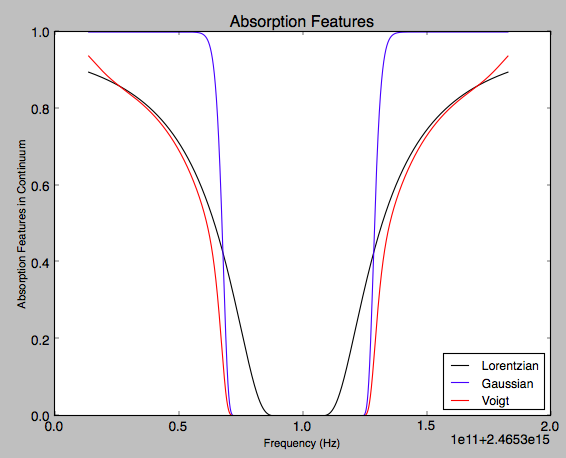
\includegraphics[width=0.66\textwidth]{figures/hw11pic2.png}
    \caption{Voigt profile.}
    \label{fig:voigt2}
\end{figure}

The absorption features due to each type of broadening is also plotted. The optical depth is given by: \\ \\
$$\tau = n \sigma s$$ 
$$ = N\sigma$$ \\

where $N$ is the column density. An absorption feature reduces the intensity of light by $e^{-\tau} = e^{-N\sigma}$ when there is no emission ($I_{\nu} = I_{\nu,0}e^{-\tau}$). The line profile function is incorporated into the cross-section $\sigma$ by the following:

$$\sigma = {\frac{\pi e^{2}}{m_{e}c}}f\phi(\nu)$$ \\

Therefore, different cross-sections can be calculated for each line profile function (using a Ly-$\alpha$ oscillator strength of $f=0.416$. The factor $e^{-N\sigma}$ by which a continuum is reduced creates the absorption feature. Again, the Voigt feature is dominated by the Gaussian at its center and by the Lorentzian wings.


\textbf{Collisional Broadening}\\

Collisional, or Pressure Broadening, is one cause of the width $\Delta\nu$ in a line profile function $\phi(\nu)$. This type of spectral line broadening arises from collisions that interfere with natural emission processes. Collisions amongst atoms in a high pressure gas can trigger the release of photons by reducing the effective lifetime of energy states, and therefore results in a steeper decay rate and the broadening of absorption lines. \\

The collision timescale is given by:

$$t_{collision} \sim t_{spontaneous\ decay} \sim {\frac{1}{A_{10}}} $$

And the collision rate is dependent on number density, cross section, and velocity:

$$A_{10} \sim n\sigma v$$ \\

In order for Collisional Broadening to dominate, a very dense gas and high velocities are needed. This is related to pressure, which is why Collisional Broadening is sometimes called Pressure Broadening. And this is also why white dwarfs produce broader spectral lines than giants of the same spectral types. \\

The cross section is also important in dictating the timescale for interaction. For fixed number density and velocity: 

$$t \propto {\frac{1}{\sigma}}$$ \\

Atoms can interact in a variety of ways. There are different collisional cross sections due to different $\vec{E}$ field drop-off rates, such as $1/r^{2}$ for the Coulomb interaction between ions or charged particles, and $1/r^{3}$ for neutral atoms (dipole field), etc. Because these fields fall off at different rates, there are different cross sections for interaction. Therefore, the time scales for Collisional Broadening depend on which type of interaction dominates, which in turn affect the shape of the line profile function. \\

The line profile function due to Collisional Broadening is a Lorentzian Profile, similar to that caused by Natural Broadening. If all 3 types of broadening mechanisms are present, then Collisional Broadening will add width to the Voigt Profile. Different mechanisms can be responsible for broadening at different distances from the line center.

\textbf{ Zeeman Splitting}\\

The Zeeman Effect concerns the splitting of electronic levels in a magnetic
field.  We've already talked a little bit about this in hyperfine 
splitting, which was caused by magnetic fields intrinsic to an atom.  We find
that a single line can split into $\sim3-27$ components, depending on the 
number of combinations of $\vec L$ and $\vec S$ there are in the atom.  The
strengths of these various lines depend on viewing geometry, and can be
polarized.  The change in energy between previously degenerate states set up
by an external $B$ field is:
$$\begin{aligned}\Delta E&\sim\mu B\sim\frac{e\hbar}{ m_ec}B\\ 
&\sim\frac{hc}{\lambda_1}-\frac{hc}{\lambda_2}\\ 
&\sim\frac{hc}{\lambda}\frac{\Delta\lambda}{\lambda}\sim\\frac{e\hbar B}{ m_ec}\\ \end{aligned}$$
Thus the fractional change in wavelength is:
$$\boxed{\frac{\Delta\lambda}{\lambda}\sim\lambda\frac{eB}{2\pi m_ec^2}}$$
In practice, we find that the various split components of the original
absorption lines are hard to resolve, and we see the effect expressed mostly
as a broadening of the original line.



\subsection{Zeeman Splitting}

 Zeeman splitting is the splitting of energy levels (and from an observational perspective, spectral lines) that occurs when an atom emits in a magnetic field. This effect is easiest to understand for atoms in the singlet state where a semi-classical treatment suffices for explaining splitting, this is called the normal Zeeman effect. For the anomalous Zeeman effect, which occurs in arbitrary spin and angular momentum transitions, a quantum mechanical treatment is necessary.   
 
 \begin{figure}[ht]
     \centering
     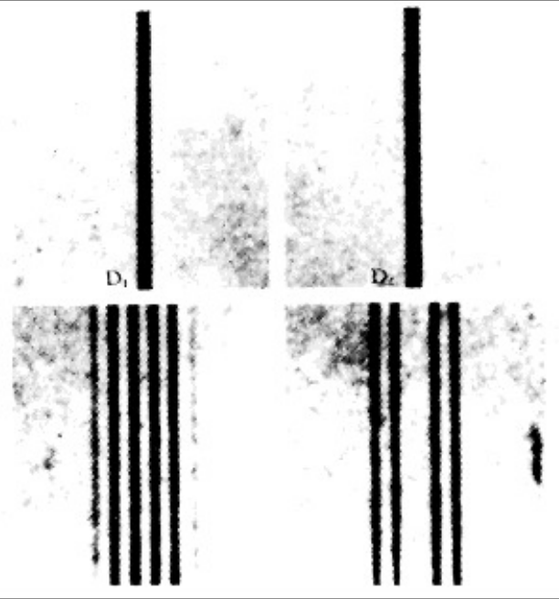
\includegraphics[width=0.33\textwidth]{figures/zeeman1.png}
     \caption{Results from the original experiment conducted by Zeeman. On left is with a magnetic field, at right is without}
     \label{fig:zeeman_exp}
 \end{figure}
 
 \subsubsection{Normal Zeeman Splitting}
 If we consider singlet transitions ($\Delta m = 0, \pm 1$) then the energy change due to magnetic field is, much like we saw when doing fine/hyperfine transitions:
\begin{equation} 
\Delta E = -\mu \cdot \mathbf{B} = - m_l \mu_e B_{ext}
\end{equation}
Only here the B field is external. $m_l$ is just the magnetic quantum number (which can range between $-l < m_l < l$ for a given orbital) and $\mu_e = e\hbar/2m_e$. In the simplest case of transition between the $l = 2$ singlet state and the $l = 1$ singlet state which would have given off a photon with frequency $\omega_0$ in the absence of an external field, this gives us $\omega_+ = \omega_0 + eB/2m_e c$, $\omega_0$, and $\omega_- =  \omega_0 - eB/2mc$. This rarely happens in nature though, so to understand how to deduce astrophysical magnetic fields from Zeeman splitting we must look a the anomalous Zeeman effect.
 \subsubsection{Anomalous Zeeman Splitting }
Anomalous splitting is the more generic case of Zeeman splitting that arises when our spin is nonzero, meaning that spin orbit coupling occurs and $m_l$ is no longer a good quantum number. In most astrophysical cases of interest the external magnetic field is much lower than the internal magnetic field so we can treat the Zeeman effect as a perturbation to the fine structure field. The perturbing hamiltonian is simply:
\begin{equation}
H'_z = -(\mu_l +\mu_s) \cdot B_{ext}
\end{equation} 
where $\mu_l$ and $\mu_m$ are the magnetic moments associated with orbital motion and spin, respectively. Since we are only looking at a perturbation, we can still use the 'good' quantum numbers for spin orbit coupling (for more on spin-orbit coupling see Rybicki and Lightman chapter 9), that is, n, l, j and $m_j$. Using that:
\begin{equation}
\mu_l = -\frac{e}{2m}\mathbf{L}
\end{equation}
\begin{equation}
\mu_m = -\frac{e}{m}{\mathbf{S}}
\end{equation}
We can redefine our hamiltonian in terms of $\mathbf{S}$ and $\mathbf{L}$ and use first order perturbation theory to find:
\begin{equation}
\Delta E = \frac{e}{2m} \mathbf{B_{ext}} \cdot  \big \langle \mathbf{J} + \mathbf{S} \big \rangle 
\end{equation}
Where we've used that ${\mathbf{J}} = {\mathbf{S}}+{\mathbf{J}}$. Though we know the expectation value of J, we need to find the one for S in this system. We can do this by noting that since $\mathbf{J}$ (total angular momentum) is constant, and $\mathbf{S}$ precesses at high frequency about this vector, the time averaged value for $\mathbf{S}$ is just the projection onto this constant vector:
\begin{equation}
\mathbf{S_{avg}} = \frac{ \big \langle \mathbf{S} \cdot \mathbf{J}\big \rangle}  {\mathbf{J}^2} \mathbf{J}
\end{equation}
We can then use that $\mathbf{J} = \mathbf{S}+\mathbf{J}$ to find an expression for this dot product in terms of quantities for which we have good quantum numbers: 
\begin{equation}
2\mathbf{S} \cdot \mathbf{J} = J^2 + S^2 -L^2 
\end{equation}
These are all quantities for which we know the eigenvalues! So we can write:
\begin{equation}
S \cdot J = \frac{1}{2}(J^2 +S^2 - L^2) = \frac{\hbar}{2}[j(j+1) +s(s+1) - l(l+1)]
\end{equation}
This can be plugged back into our expression for $\mathbf{S_{avg}}$, which can subsequently be plugged back into our expression for $\Delta$ E to give:
\begin{equation} 
\Delta E = \frac{e \hbar B_{ext}}{2m_ec} \left(1+ \frac{j(j+1) +s(s+1) +l(l+1)}{2j(j+1)}\right) m_j =  \frac{e \hbar B_{ext}}{2m_ec} g(j, s, l) m_j
\end{equation}
where g(j,s,l) is the quantity in the parenthesis and is called the Lande g factor. For the purposes of observational astronomy, these gs can all be looked up in a table. 

\begin{figure}
    \centering
    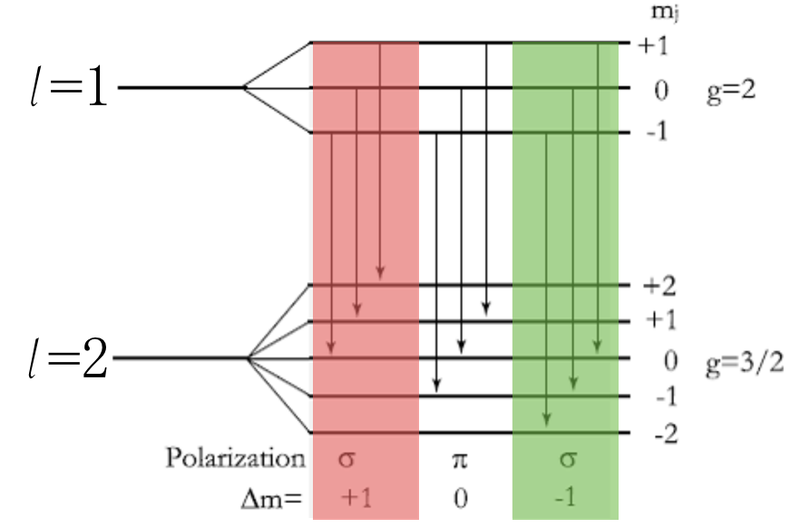
\includegraphics[width = 0.45\textwidth]{figures/800px-Zeeman_Splitting.png}
    \caption{An illustration of allowed energies due to the Zeeman effect for the l=1 l=2 transition. Note the polarization associated with varying changes in $m_j$. Figure modified from L. Woolsey by A. Parsons}
    \label{fig:zeeman}
\end{figure}
 \subsubsection{Observing the Zeeman Effect}
 To get an idea for the change in energy caused by Zeeman splitting we can take a typical magnetic field for the ISM of $10\mu G$ and use the table in Heiles et al. (see references above), to find the shift in the 21 cm hyperfine transition to be on the order of 10 Hz. This is an incredibly small shift and for most astrophysical systems (masers being the exception), is impossible to measure directly. However, we can measure even small shifts due to Zeeman splitting utilizing the polarization of the split lines. Transitions that change values of $l$ but maintain the same value of $m_j$ are $\pi$ polarized where transitions that have a $\Delta m_j$ of $\pm 1$ are $\sigma$ polarized. We can then use that these $\sigma$ polarized lines are elliptically polarized (meaning they are both circular and linearly polarized) to measure the right and left circular polarization of our signal. Adding these two parameters gives the Stokes I parameter where subtracting them gives the Stokes V parameter. If there is no magnetic field we expect our Stokes V parameter to be 0 however, however if there is, the measured V spectrum will be off the form:
 \begin{equation}
 V(\nu) = \frac{dI (\nu)}{d \nu}bB_{\parallel}
 \end{equation}
 Where  $B_{\parallel}$ is the line of sight component of the B field and $I(\nu)$ is the Stokes I parameter. This technique makes it possible to measure Zeeman splitting in the ISM.  

\subsection{Class Notes}

A question I had -- what do we mean by $\phi(\nu) \sim \frac{1}{\Delta \nu}$. The function is in some ways a PDF. It has to have the property that:

\be
1 = \int \phi_\nu d\nu
\ee

We can think of $\phi(\nu)$ being a measure of the spread of the profile. This allows us to think of $\Delta \nu$ as $1/\Delta \nu$. 

Also note that we can approximate the cross section:

\begin{equation}
    \sigma_\nu = \frac{A}{8\pi} \lambda_0^2 \phi(\nu)
\end{equation}

This cross-section results in attenuating light differently at different frequencies. This leads to the absorption. 


%%%%%%%%%%%%%%%%%%%%%%%%%%%%%%%%%%%%%%%%%%%%%%%%%%%%%%%%%%%%%%%%%%%%%%%%%%%%%%
%%%%%%%%%%%%%%%%%%%%%%%%%%%%%%%%%%%%%%%%%%%%%%%%%%%%%%%%%%%%%%%%%%%%%%%%%%%%%%
%%%%%%%%%%%%%%%%%%%%%%%%%%%%%%%%%%%%%%%%%%%%%%%%%%%%%%%%%%%%%%%%%%%%%%%%%%%%%%
\newpage
\section{September 24, 2020: Estimating Atomic Transition Strength}

\subsection{Estimating the Strength of Atomic Transitions}

Previously, we introduced $A_{21}$, which can be related to $B_{12}, B_{21}$ (absorption and stimulated emission, respectively). We had:

\begin{equation}
    A_{21} = \frac{2 h \nu^3}{c^2} \underbrace{B_{21}}_{\text{stimulated emission}}
\end{equation}

We also had:

\begin{equation}
    g_1 B_{12} = g_2 B_{21}
\end{equation}

We also showed that we could express the cross section for absorbing  a photon as:

\begin{equation}
    \boxed{\sigma_{12} \sim \frac{\lambda^2}{8\pi} \frac{A_{21}}{\Delta \nu}}, \text{ where } \frac{1}{\Delta \nu} \rightarrow \phi(\nu)
\end{equation}

\textbf{Estimating transition strengths boils down to estimating $A_{21}$!} When we have atoms in an excited state $E_2$, the number exponentially decays to energy state $E_1$. The half life is characterized by the timescale. We can relate this half-life to the $A_{21}$ as $t_{life} = A^{-1}_{21}$. This is how we define the Einstein $A$ coefficient. 

Remember when we did the semi-classical derivaiton of the Hydrogen atom? It turns out we can use that model to estimate $A_{21}$ for an electron in the second excited state compared to the ground state. We can express this as (treating radiated power classically):

\begin{equation}
    t_{life} \sim \frac{E}{P} \times \frac{3}{4}(1 \text{ Rydberg })
\end{equation}

How do we estimate power? Larmor radiation!

\begin{equation}
    P = \frac23 \frac{e^2 a^2}{c^3}
\end{equation}

This gets pretty dang close! This gives us $A_{21} \sim 5 \times 10^{8} \s^{-1}$. We can now derive scaling relationships with energy. If we have a good value to scale that off of, we can do really well!

\textbf{Scaling Relations:}\\

Recall: $A_{21}^{-1} \sim E/P$. We can write $E = \hbar \omega$. Can we get a frequency for power? Recall Larmor power has acceleration, giving us an angular frequency, though not obviously. We said that $a = v^2 / r$ in our semi-classical derivation, so we could think of that for our angular frequency! We then get $P \sim \frac{e^2 r^2 \omega^4}{c^3}$. But a charge separated by a distance ($er$) is a dipole (the dipole moment of the hydrogen atom!). Thus, $P \sim d^2 \omega^4 c^{-3}$. This leaves us with:

\be
\boxed{A_{21} = \frac{d^2 \omega_0^3}{\hbar c^3}}
\ee

Note that in the above equation, $d$ is the dipole moment and $\omega$ is the frequency of light. Let's try estimating this $A_{21}$ for $H\alpha$. 

\be
\Delta E = 1 \text{ Ryd } (1/4 - 1/9) = (5/36) \text{ Ryd }
\ee

Compared to $Ly\alpha$ at $3/4 \text{ Ryd }$., giving us:

\be
\frac{\omega_{0,H\alpha}}{\omega_{0,Ly\alpha}} = \frac{5}{27}
\ee

The dipole moment is $d \sim e a_0$ where $a_0 = \frac{n^2 \hbar^2}{m_e e^2}$. This gives:

\be
    A_{21} \propto A_{21,Ly\alpha} \left(\frac{n=2}{n=1}\right)^4 \left(\frac{5}{27}\right)^3 \sim 5 \times 10^{7}
\ee

But can we scale to fine and hyperfine transitions? Recall that the magnetic moments are $\mu_e = \frac{e \hbar}{2 m_e c}$ and $\mu_p = \frac{e \hbar}{2 m_p c}$. Can you substitute this in for electric dipole above? This would give:

\be
\frac{A_{21,mag}}{A_{21,elec}} \sim \frac{\mu_e^2}{d^2} \sim \left(\frac{e \hbar}{m_e c e a_0}\right)^2 \sim \alpha^2
\ee

Therefore the Einstein coefficients for magnetic dipoles get damped by $\alpha^2$ compared to electric dipoles. For example, we can estimate $A_{21}$ for the 21-cm line (magnetic):

\begin{equation}
    \frac{A_{21,21cm}}{A_{21,Ly\alpha}} = \alpha^2 \underbrace{\left(\frac{120 \nm}{ 21 \cm}\right)^3}_{\text{correct for } \omega^3} = 1\times 10^{-23} 
\end{equation}

Plugging in the $A_{21,Ly\alpha}$, we get:

\be
A_{21,21cm} = 5\times10^{-15} \s^{-1}
\ee

which is correct to a factor of 2. 

Let's do one last thing: \textbf{radio recombination lines!} These are very high $n$ transitions like $n=110 \rightarrow 109$. These are really small eneryg differences. Remember that $\omega^3$ term in the scaling? For radio recombination lines, $A_{21} \propto n^4 n^{-9} \propto n^{-5}$. The $1/n^9$ comes from difference in $1/n^2$ dependence of frequency in hydrogen being like a derivative.

Lastly, what about quadrupole transitions? This is a pair of dipoles associated with one another. Whereas the electric field of the monpole $\propto r^{-2}$, dipoles $\propto r^{-3}$. Quadrupoles give:

\be
\vec{E}_{quad} \propto \frac{q}{r^2}\frac{s^2}{r^2}
\ee

Kinks in the $\vec{E}$ field carries the power, so power for quadrupoles scale as the $E$ field squared:

\be
\frac{P_{quad}}{P_{dipole}} \sim \frac{\frac{s^4}{r^4}}{\frac{s^2}{r^2}}
\ee

We want to see, for different transitions, how does the power compare? We end up finding that: 

\be
\frac{P_{quad}}{P_{dipole}} \sim \frac{s^2}{\lambda^2}
\ee

Likewise, 

\be
\frac{A_{21,quad}}{A_{21,di}}\sim \frac{s^2}{\lambda^2}
\ee

Let's estimate numerically an Einstein $A$ for a quadrupole:

The first rotational transition has a $\lambda = 28 \mu m$:

\be
A_{12,H_2} = A_{21,Ly\alpha} \underbrace{\left(\frac{0.5 \times 10^{-8} \cm}{28 \times 10^{-4} \mu m}\right)^2}_{\text{s/}\lambda \text{ term }} \underbrace{\left(\frac{120 \times 10^{-7} \cm}{28 \times 10^{-4} \cm}\right)^{3}}_{\omega^3 \text{ term }}
\ee



\subsection{Additional Notes}

\subsubsection{ Einstein A's for Lyman Alpha}

Recall from Einstein Coefficients that $\ato$ is a measure of the probability of decay per unit time, so
$\ato^{-1}$ is approximately the lifetime of an atom in an excited state.  This should be about
equal to the energy of the electron state divided by the average power radiated
by an electron being accelerated:
$$\ato^{-1}\sim\frac{E}{ P}\sim\frac{\hbar\omega_0}{{\frac23}\frac{e^2\ddot x^2
}{c^3}}
\sim\frac{3\hbar\omega_0c^3}{2(e\ddot x)^2}$$
Now $e\cdot\vec x=\vec d$ (the electric dipole moment) and
$\ddot x\sim\omega_0^2x$ for a spring, so:
$$\ato^{-1}\sim\frac{3\hbar\wz c^3}{2d^2\wz^4}$$
$$\boxed{\ato\sim\frac{2d^2\wz^3}{3\hbar c^3}}$$
For H: 
$d\sim ea_0$ and $\lambda_\lya=1216\angstrom$ 
so:
$$\ato\sim5\e8s^{-1}$$

\subsubsection{ Magnetic Dipole for Lyman Alpha}

The magnetic dipole of an electron is:
$$\mu_e=\frac{e\hbar}{ m_ec}$$
Thus we can estimate the ratio of $\ato$ for magnetic dipole transitions to
that of electric dipole transitions:
$$\frac{\ato\eval{mag}}{\ato\eval{elec}}\sim\left(\frac{\mu_e}{ d}\right)^2
\sim\left(\frac{e^2}{\hbar c}\right)^2\sim\alpha^2$$
This tells us that the magnetic dipole states (that is, fine and hyperfine
states) are longer lived than electric dipole states by a factor of $\alpha^2$.
$$\frac{\ato\eval{21cm}}{\ato\eval{Ly\alpha}}\sim\alpha^2
\left(\frac{1216\angstrom}{21cm}\right)^3$$
$$\ato\eval{21cm}\sim6\e{-15}s^{-1}$$
The actual value is $2.876\e{-15}s^{-1}$.

\def\mfe{\mathfrak{E}}
\subsubsection{ Electric Quadrupole}

If one is nearby a rotating quadrupole, one sees the $\mfe$  (electric)
field rotating rigidly.
However, from far away, there are kinks in the field, resulting in a retarded
potential.  The radiation nearby goes as $r_{near}\sim\lambda$.  For a monopole,
the electric field is $\mfe\sim\frac{q}{ r^2}$.  For a dipole, it is 
$\mfe=\frac{q}{r^2}
\frac{s}{ r}$, where s is the charge separation.  For a quadrupole: 
$$\mfe=\frac{q}{ r^2}\left(\frac{s}{r}\right)^2$$
Since $P\propto \mfe^2$, the ratio of the powers emitted by a
quadrupole vs. a dipole should be:
$$\frac{P_{quad}}{ P_{di}}\sim\left(\frac{s}{ r}\right)^2
\sim\left(\frac{s}{\lambda}\right)^2$$
An acoustic analogy: a kettle whistle is a monopole, a
guitar string is a dipole, and a tuning fork (with its two out-of-phase
prongs) is a quadrupole.\\

Anyway, since $\ato\sim\frac{P}{E}$,
$$\boxed{\frac{\ato\eval{quad}}{\ato\eval{di}}
\sim\left(\frac{s}{\lambda}\right)^2}$$
Thus $28\mu m$, the lowest quadrupole rotational transition of
$H_2$, should have an $\ato$ of about:
$$\ato\eval{28\mu m}\sim\ato\eval\lya\left(\frac{s}{\lambda_{H_2}}\right)^2
\left(\frac{\lambda_\lya}{ \lambda_{H_2}}\right)^3
\sim\ato\eval\lya\left(\frac{a_0}{ 28\mu m}\right)^2
\left(\frac{1216\angstrom}{ 28\mu m}\right)^3
\sim7\e{-11}s^{-1}$$
The actual value is $3\e{-11}s^{-1}$.

\subsubsection{ Radio Recombination Lines}

In HI, the $n=110\to n=109$ transition has a wavelength of 6 cm.  We can
estimate its $\ato$:
$$\ato\eval{6cm}\sim\ato\eval{Ly\alpha}
\underbrace{\left(\frac{1216\angstrom}{6cm}\right)^3}_{\text{change in} \lambda}
\underbrace{\left(\frac{a_{110}}{ a_0}\right)^2}_{\text{change in atom size}}$$
\def\bra#1{\langle #1|}
\def\ket#1{|#1\rangle}
This presents the question of which dipole moment to use.  It turns out
we must use $\bra{i}\vec k\cdot\vec r\ket{f}$.

\subsubsection{ Back to Sigma}

$$\sigot\eval{\text{line center}}\sim\frac{\lambda^2}{8\pi}\frac{\ato}{\Delta\nu}$$
Now $\Delta\nu\sim\nu$ for Doppler broadening, and $\ato\sim\nu^3$, so for
electric and magnetic dipole transitions:
$$\sigot\sim\lambda^0$$
So the cross-section for these transitions does not depend on wavelength.

\subsection{Class Notes}

The big takeaway is that, knowing a single $A$ coefficient is enough to derive the other ones using scaling relations.

\begin{equation}
    A_{21}=\frac{8 \pi^{2} \nu^{2} e^{2}}{m_{e} c^{3}} \frac{g_{1}}{g_{2}} f_{21}
\end{equation}

\be
A \sim t^{-1} \sim P/E
\ee

\be
a \sim \nu^2 \rightarrow P \sim \nu^4 \rightarrow P/E \sim \nu ^3
\ee

One thing to note is that molecules like O$_2$ don't have a dipole moment whereas things like CO do. Aaron noted that O$_2$ does have a quadrupole moment.


%%%%%%%%%%%%%%%%%%%%%%%%%%%%%%%%%%%%%%%%%%%%%%%%%%%%%%%%%%%%%%%%%%%%%%%%%%%%%%
%%%%%%%%%%%%%%%%%%%%%%%%%%%%%%%%%%%%%%%%%%%%%%%%%%%%%%%%%%%%%%%%%%%%%%%%%%%%%%
%%%%%%%%%%%%%%%%%%%%%%%%%%%%%%%%%%%%%%%%%%%%%%%%%%%%%%%%%%%%%%%%%%%%%%%%%%%%%%
\newpage
\section{September 29, 2020: Atomic and Molecular Quantum Numbers}

\subsection{What are quantum numbers?}

We know from quantum mechanics that observable quantities are quantized. Each quantum number corresponds to an observable quantity or combination of quantities and describe the quantized states that characterize a system. That is, they are the set of numerical values that give acceptable solutions to the Schrodinger equation for that system. There is no single set of quantum numbers that completely describes every system; different types of systems are fully described by different quantum numbers.

\subsection{Quantum numbers in an atom}

An electron in an atom is described completely by four quantum numbers: $n, \ell, m,$ and $s$. (Fewer quantum numbers can be made to describe an electron if you choose carefully, since the spin-orbit interaction relates some of these numbers. However, this is the standard way.)

\begin{itemize}
    \item The \textbf{principal quantum number} $n = 1,2,...$ describes the electron's energy level, or shell. As $n$ increases, the average distance of the electron from the proton increases.
\end{itemize}

\begin{itemize}
    \item The \textbf{orbital quantum number} $\ell = 0, 1, 2, ... n-1$, also called the azimuthal quantum number or the angular quantum number, describes the shape (or subshell) of the electron's shell. In chemistry,  $\ell = 0$ is called the s orbital, $\ell = 1$ is called the p orbital, $\ell = 2$ is called the d orbital, and $\ell = 3$ is called the f orbital. $\ell$ corresponds to the orbital angular momentum of the electron as follows:

\be
L^2 = \hbar^2 \ell (\ell + 1)
\ee
    \begin{itemize}
        \item The value of $\ell$ ranges from $0$ to $n-1$ because the first p orbital appears in the second $(n=2)$ shell.
    \end{itemize}
\end{itemize}

\begin{figure}[ht]
    \centering
    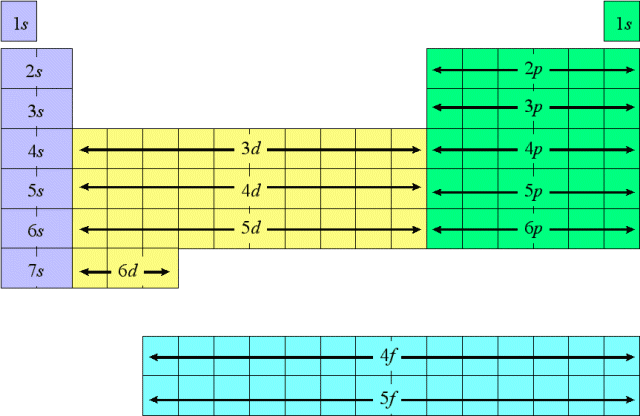
\includegraphics[width = 0.75\textwidth]{figures/Periodictable.png}
    \caption{Outline of the periodic table of elements showing the orbital in which that element's valence electrons are found.}
    \label{fig:periodic}
\end{figure} 

\begin{itemize}
    \item The \textbf{magnetic quantum number} $m_\ell = -\ell, 1 - \ell, 2 - \ell, ..., 0 ..., \ell - 2, \ell - 1, \ell$ describes the specific orbital within the subshell. The s subshell contains just one orbital: $m_\ell = 0$ is the only allowed value. The d subshell contains five orbitals, since $m_\ell$ can range from $-2$ to $+2$. $m_\ell$ corresponds to the projection of the electron's orbital angular momentum along a specified axis:
    
    \be
    L_z = \hbar m_\ell
    \ee
    
\end{itemize}

\begin{itemize}
    \item The \textbf{spin projection quantum number} $m_s = - s,1 - s,2 - s,...,s - 2,s - 1,s$ describes the spin (intrinsic angular momentum) of the electron within an orbital. Here $s$ is the \textbf{spin quantum number}, an intrinsic property of a particle, and $m_s$ is related to the projection of the spin angular momentum $S$ along a specified axis:
    
    \be
    S_z = \hbar m_s
    \ee
    \begin{itemize}
        \item An electron has spin number $s = \pm 1/2$, so the allowed values of $m_s$ are $-s$ and $+s$, or $m_s = - 1 / 2$ or $1 / 2$. Because electrons are fermions (i.e. they have a half-integer spin), they behave according to the Pauli exclusion principle, so an orbital cannot contain two electrons with the same spin. 
        
        \item Example: The valence electron of an aluminum atom is located in the 3p1 orbital, so it has quantum numbers n = 3 (3rd electron shell), $\ell = 1$ (p orbital subshell), $m_\ell = -1, 0,$ or $1$, and $m_s = - 1 / 2$ or $1 / 2.$

    \end{itemize}
\end{itemize}


\subsection{Total Angular Momentum Numbers}

The spin-orbit interaction is caused by electromagnetic interaction between the electron's spin and the magnetic field generated by the electron's orbit around the nucleus, shifting an electron's energy levels slightly. This can be thought of as a Zeeman effect due to the internal magnetic field of an atom. One consequence of the spin-orbit interaction is that the orbital angular momentum L and the spin angular momentum S are no longer independent, and a new set of quantum numbers should be used that describe the total angular momentum.

\begin{enumerate}
    \item The principal quantum number as before.
    
    \item The \textbf{total angular momentum quantum number} $j = |\ell \pm s|$ gives the total angular momentum as:

\be
J^2 = \hbar^2 j(j+1)
\ee

    \item The \textbf{projection of} $J$ along a specified axis $m_j = - j,1 - j,2 - j,...,0,...,j - 2,j - 1,j$ satisfies $m_j = m_\ell + m_s$ and $|m_\ell + m_s \leq j|$
    
    \item The \textbf{parity} is positive for states that come from even $\ell$ and negative for states that come from odd $\ell$, such that $P = (-1)^\ell$.
\end{enumerate}

\subsection{Quantum Numbers in Diatomic Molecules}

\subsubsection{Rotation}

A diatomic molecule may rotate about a direction perpendicular to the bond axis, giving rise to angular momentum $N$. However, a molecule also possesses electronic angular momentum $L$. These two momenta couple to make a \textbf{total angular momentum} $J = N + L$ which is conserved, though $N$ and $L$ are not themselves conserved since one type of angular momentum could be converted to the other. The notation gets a bit weird here: in the electron case capital letters denote actual angular momenta, i.e. the factors of $\hbar$ are in there, but in the case of rotating molecules a capital $J$ is used as a quantum number directly. That is, you'll often see transitions labeled $J = 1 \rightarrow 0$, meaning that a molecule has moved from the first excited rotational state to its ground state. The total angular momentum is given by: 
\be
J(J + 1)h^2
\ee

Since $N$ must be perpendicular to the bond axis to be nonzero, $J_z = L_z$ and $L_z$ is conserved, too, meaning that $M_L$ is is a good quantum number to use to describe the electronic contribution to the total angular momentum. Since the energy of the system is the same whether $M_L$ is positive or negative, $\Lambda = | M_L |$ is usually used instead. Of course, there may also be a small contribution from electron spins, which is similarly parameterized as $\Sigma = |M_s|$. The total is again conserved, with $\Omega = \Sigma + \Lambda$ describing the \textbf{total angular momentum projected onto the bond axis.}

\subsubsection{Vibration}

A diatomic molecule vibrates approximately as a simple harmonic oscillator, and its vibration state can be described by a single quantum number $\nu$, where $E = (\nu + 1 / 2)h\omega$ are the energy levels. Anharmonic terms proportional to $\nu^2$ or higher order terms are possible but generally very small for diatomic molecules.

\subsubsection{Rovibrational Spectra}

The total internal energy of a molecule is the sum of its rotational and vibrational energy. The selection rule for vibration is  $\Delta \nu = \pm 1$. In reality contributions from $\Delta \nu = \pm 2, \Delta \nu = \pm 3$, etc. also arise in a spectrum at much lower energies due to the anharmonic terms. For rotation, $\Delta J = 0, \pm 1$ is the selection rule; however, in a linear molecule $\Delta J = 0$ is only allowed if there is angular momentum perpendicular to the rotation axis, which is possible either if a molecular bending mode is excited or if there's an unpaired electron and $\Omega \neq 0$ (as in, for example, the molecules NO and OH).

A rovibrational spectrum is classified into three branches, P, Q, and R, which correspond to $\Delta J = - 1$ (low energy), $0$ (medium energy), and $1$ (high energy), respectively.

\begin{figure}[ht]
    \centering
    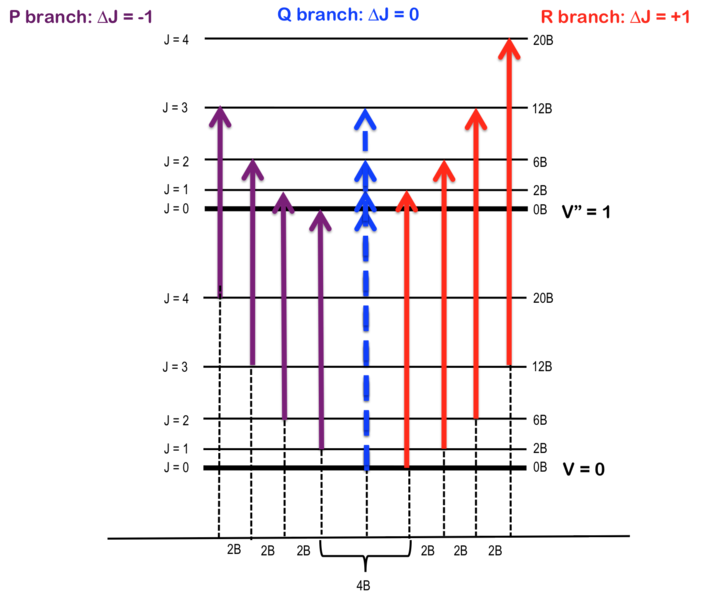
\includegraphics[width = 0.75\textwidth]{figures/Pqr.png}
    \caption{Schematic diagram of rovibrational transitions with the P, Q, and R branches labeled.}
    \label{fig:pqr}
\end{figure}

\begin{figure}[ht]
    \centering
    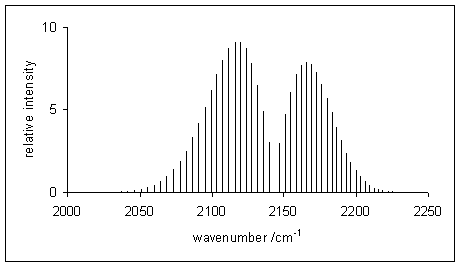
\includegraphics[width = 0.75\textwidth]{figures/Co.png}
    \caption{Rovibrational spectrum of carbon monoxide (CO).}
    \label{fig:rovibrational}
\end{figure}

\subsection{Class Notes}


``Be excellent to each other and then strike an air guitar pose.''

The entire magic of the class, as a reminder, is embedded in the Einstein coefficients. And remember the scaling and a typical number:

\be
A \propto d^2 E^3 
\ee

\be
A_{\text{Ly}\alpha} = 5 \times 10^{8} \s^{-1}, \tau_{\text{Ly}\alpha} = 2 \text{ ns}
\ee

Also, most of the time you don't need ot mess with the dipole term since that is pretty much the same for electronic transitions, so we really only care about the frequency term. 

Now, this week we dive into rotational and vibrational transitions. 

Case study of the phosphine in Venus, with the caveat that we have no idea what phosphine is since we are not chemists.

You have some atoms that are linked to each other (often, you need to be in a dense environment, such as in a molecular cloud. Atoms have to find each other!). You also need pretty cool environments to have molecules, too. Cool, here could be hot enough to cook you, just not compeltely dissociating all the molecules. Let's start with rotation:

Picture two atoms attached by a spring. Perhaps they spin, too, around the center of mass. This gives an angular momentum $L$. This looks a lot like hydrogen, but we need more detail. One thing we need to know is the spacing, so let's talk about that.

Why do atoms settle in at a certain spacing? We have to have some equilibrium state such that the potential energy has a minimum where they are happy ot sit. 

\begin{figure}
    \centering
    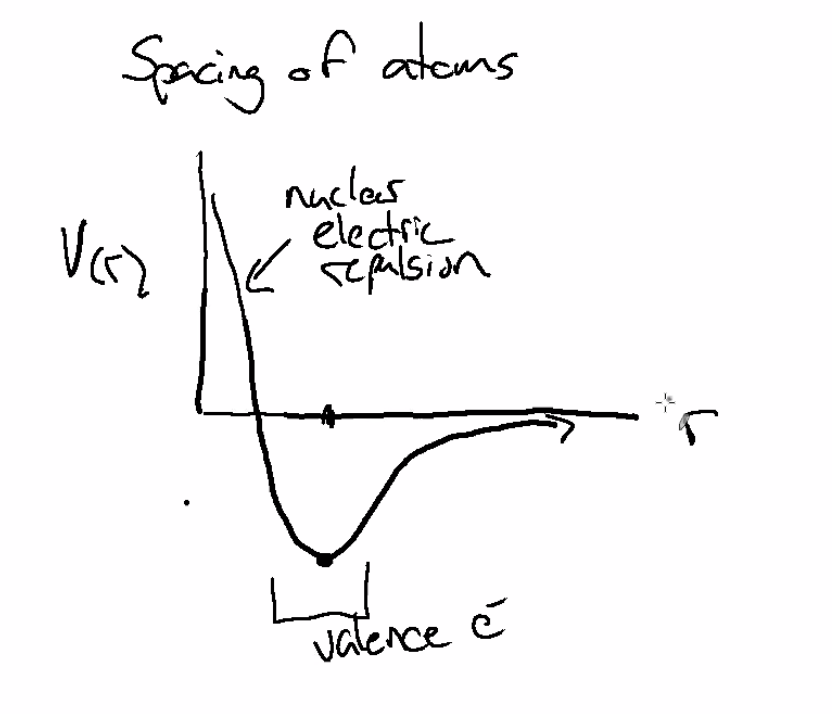
\includegraphics[width=0.75\textwidth]{figures/Screen Shot 2020-09-29 at 11.28.49 AM.png}
    \caption{Typical potential for a molecule. Note at large $r$ we lose the electric force.}
    \label{fig:pot}
\end{figure}

This is far too complicated to deal with, so we will model it as a harmonic potential. 

\be
V \propto \frac12 k \left(\Delta r\right)^2
\ee


This works because we can center it at some distance (talk about perturbations around that). Also, for any potential with a local minimum has a first derivative equal to 0, which is fine because neither did our potential! We do have a second derivative, however, which is the leading term of a local minimum. Thus, the harmonic potential matches our potential to its leading term in a Taylor expansion. 

\begin{figure}
    \centering
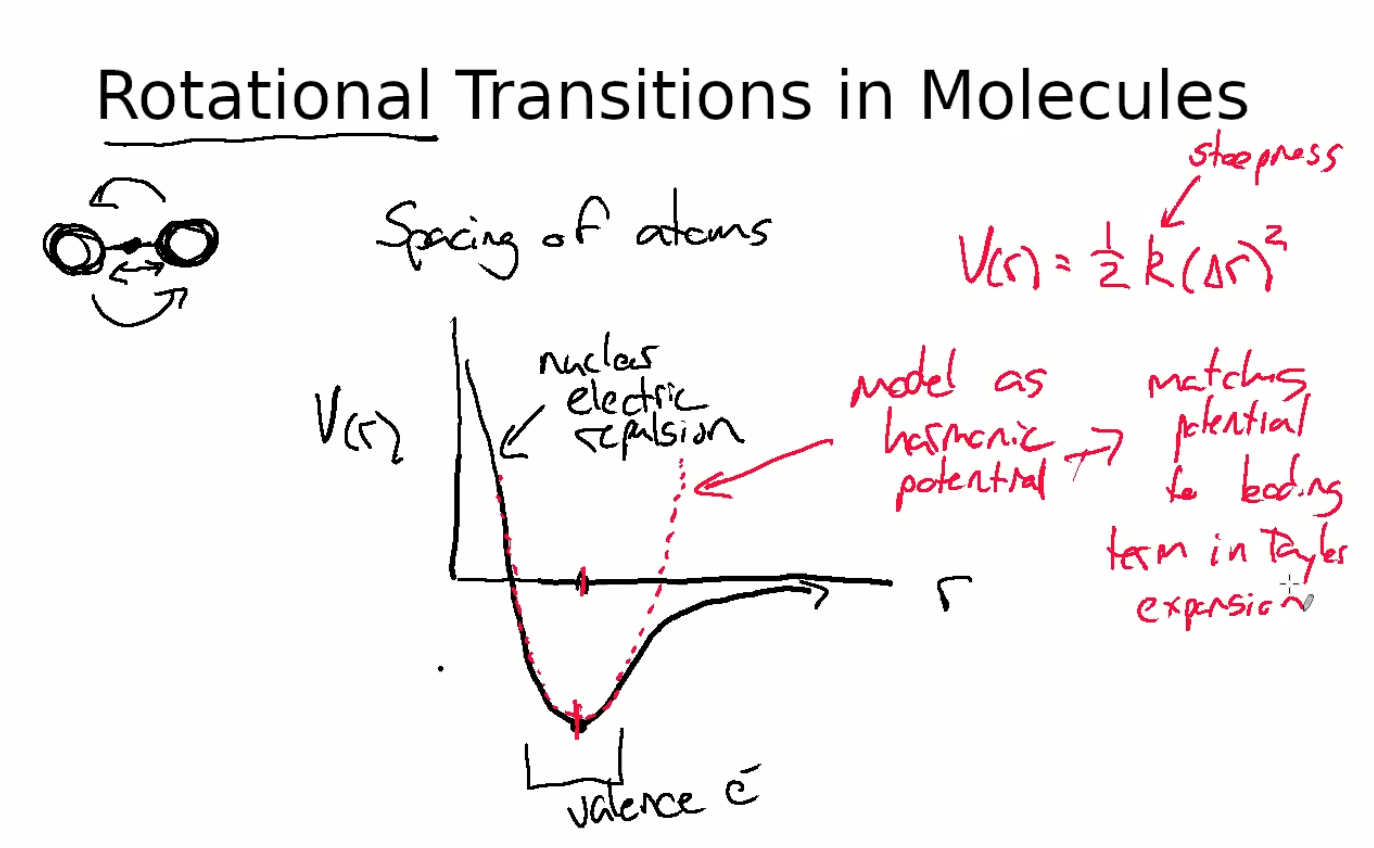
\includegraphics[width=0.75\textwidth]{figures/Screen Shot 2020-09-29 at 11.32.41 AM.png}
    \caption{}
    \label{fig:pot2}
\end{figure}

So how far apart are the two? It makes sense to say it's approximately 2 Bohr radii! that means that $r \sim 2 a_0$. this works for molecules too since the nuclear charge pulls HARDER on the electrons, so even if we have more electrons, we have stronger repulsion. The outside electron determines the radius, and it itself is shielded from the nucleus. Thus, we have pretty much just Coulomb attraction and repulsion. It's a rough rule of thumb, but it works. This all amounts to centering our potentail at 2 Bohr radii.

Let's start with diatoms, since it generalizes. Key ingredients:

\begin{enumerate}
    \item Quantize angular momentum.
    \item Calculate our angular velocity $\omega$. 
    \item Characterize our rotational energies. 
\end{enumerate}

Let's start by quantizing angular momentum. In classical Bohr atom, we used $n$. Here, we use $J$. We do this because $J$ is the {\textbf total angular momentum}. This accounts for the rotational angular momentum and spin-angular momentum and others:

\be
J = \underbrace{L}_{\text{rotational}} + \underbrace{S}_{\text{spin}} + \underbrace{N}_{\text{orbital electron angular momentum}}
\ee

Internally, the molecule can bounce $L, S$, and $N$. These are thus not conserved. We use $J$ since it \textbf{is} conserved. We now have:

\be
|\vec{L}| = J\hbar
\ee

Also remember that:

\be
L = \sum m r_{cm} v_\perp
\ee

Assuming uniform, solid body rotation:

\be
V_\perp = r_{cm} \omega
\ee

Thus, 

\be
L = \sum m r_{cm}^2 \omega 
\ee

Our frequency doesn't change, so we have:

\be
L =  \omega \underbrace{\sum m r_{cm}^2}_\text{moment of inertia} = I \omega
\ee

We thus have:

\be
L = I \omega = J \hbar
\ee

\be
E = \sum \frac12 m v_\perp^2 = \sum \frac12 mr^2 \omega^2 = \frac12 I \omega^2 = \frac{1}{2I} |\vec{L}|^2
\ee

Thus:

\be
E(J) = \frac{\hbar^2}{2I}J^2
\ee

Note that $J^2$ is note actually an eigenstate of the energy operator. We will accept as a fact that the real energy eigenstate is $J(J+1)$:


\be
\boxed{{E(J) = \frac{\hbar^2}{2I}J\left(J+1\right)}}
\ee

As long as we can figure out $I$, we are good! \textbf{For a diatomic molecule}, the algebra is annoying but simplifies to:

\be
\mu = \frac{m_1 m_2}{m_1 + m_2}
\ee

And therefore, with $r$ as the intermolecular spacing:

\be
I = \mu r^2 
\ee

So let's try carbon monoxide! This is an important molecule in space -- think of the CNO cycle. This molecule has a very similar binding energy to $H_2$, and thus it is very common in hydrogen molecular clouds. We can thus use it as a tracer for hydrogen! Why would we not use hydrogen itself? Let's come back to that...

Let's call carbon $m_1$ and oxygen $m_2$. This makes our reduced masS:

\be
 \mu_{CO} = \frac{\left(12 m_p \right) \left(16 m_p \right)}{\left(12+16\right) m_p} \approx 6.85 m_p
\ee


What about our moment of inertia, assuming a 2 Bohr radii separation? 

\be
I_{CO} = \mu_{CO} \left(\frac{2\hbar^2}{e^2 m_e}\right)^2
\ee

Let's use this to give a specific transition, say $J=1\rightarrow0$. This is the lowest rotational transition in carbon-monoxide. Remember:

\be
E_{J=1\rightarrow0} = \frac{2\hbar^2}{2I}\left(2 - 0\right) = \frac{5e^4 m_e^2}{128\hbar^2 m_p}
\ee

In c-g-s units, we have $e = 5e-10 \unit{esu}$, $m_e = 1e-27 \unit{g}$, $\hbar = 1e-27 \ergs \s$, and $m_p = 2e-24 \unit{g}$. This should come out to be around 

\be
E_{J=1\rightarrow0} = 7 \times 10^{-16} \ergs
\ee

Turning this to a frequency, we have:
\be
\nu_{J=1\rightarrow0} \sim 100 \unit{GHz}
\ee

The actual answer is around $115$ GHz. The only thing we had to guess in the entire derivation is the $2 a_0$. Note that this process, more or less in reverse, is how chemists measure interatomic spacing. 

{\large \textbf{Note that this will likely be a question on the final exam! A good practice case would be ammonia (NH3)}}. We can calculate the moment of inertia for a pyramid, for example, and do the same thing (since it is a different shape). The same can be true for CH4, for example. HOWEVER, you could not tell between ,say PH3 and NH3 since they are geometrically similar. 

What about some higher order stuff? What do we mean by this? It turns out that $\Delta J$ is usually $\pm 1$. This isn't to say anything else is impossible, but this is strongest. Why? It's the primary transition/has the strongest pathway -- not sure what this means, but guessing it's a ``sum over all paths'' analogy of quantum mechanics. Note that the $\pm 1$ change is a dipole transition that makes one photon. This photon has an angular momentum, so the easiest way to have a transition is to make a photon with an angular momentum that takes away said angular momentum from the system. This dipole transition is a quantum mechanical equivalent of Larmor radiation. 

However, if you do not have a dipole (say a quadrupole), then you can't have easy Larmor radiation (self-cancellation makes it way harder). You need another thing to happen (a new pathway). For this reason, this is sometimes called a ``forbidden'' transition. This does not mean it cannot happen, but it's way weaker. In a quadrupole, the $\Delta J = 1$ is shielded, and the $\Delta J = \pm 2$ is strongest for quadrupoles.

These sets of rules basically boil down to conserving quantum numbers. Each pathway conserves quantum numbers, and the easiest way is to change a single quantum number at a time if you are able to do that. If you cannot do that, you need other ways that change multiple numbers at the same time by, say, rearranging a spin state to allow replace rotational angular momentum while the photon is also walking away. 

All together, we call these {\textbf selection rules}. For this class, this boils down to $\Delta J = \pm 1$ for dipole molecules (asymmetric molecules). Symmetric molecules like $H_2$ don't have a dipole moment, so you must have a quadrupole. The selection rules for quadrupoles is $\Delta J = \pm 2$. There are way more, but it is difficult to remember all of them. All that matters is the concept -- these are the rules that ensure quantum numbers are conserved with the least jiggling around. If you violate a selection rule, you're a ``forbidden transition'' and are much weaker than normal transitions. 


Enough with rotational transitions -- let's talk about vibrational transitions. 

These are transitions in which the atoms are moving with respect to one another, not just co-rotating. The classic case is modelling it as a spring, with two atoms connected with a spring constant $k$. They can vibrate in a bunch of different ways (degrees of freedom) such as flexing [note that water in a microwave is the flexing transition], contracting, or other ways (exotic ways, such as tunneling through the plane of hydrogen in a molecule like NH3). 

Modeling these all as harmonic oscillators, we use a potential like $\frac12 k x^2$. We then get the eigenstates with solutions (using $n$ as the harmonic oscillator eigenstates):

\be
E(n) = \hbar \omega_0 \left(n + \frac12\right)
\ee

where $\omega_0 = \sqrt{k/m}$. Because these energy states scale linearly with $n$, we have all changes in $\Delta n$ being $\hbar \omega$. We don't care if it is $n=2\rightarrow1$ or whatever -- we cannot tell! We can calculate the characteristic energy of one of these transitions, though, only knowing $\omega_0$. We can normally get the mass, so we care about $k$. In a diatomic molecule, we just use $m = \mu$. What is $k$? 

Well, why do we have a potential at all? What we see near the minimum is the balance between the nuclear forces and the electric force. Roughly, we might say:

\be
 F = -k x \rightarrow F \sim \frac{(2e)(2e)}{r^2}
\ee

Where we roughly say that 2 electrons are involved in the interaction, and $r$ is the bond length of the molecules, so roughly $2 a_0$. Crunching the numbers, we get, in c-g-s units:

\be
k \sim \frac{4e^2}{(2 a_0)^3} \sim 1 \times 10^{6} \g \s^{-2}
\ee

For CO, we know that $n=1\rightarrow0$ has $\omega_0 = 64$ THz. Saying that $\omega_0 = \sqrt{k/\mu_{cO}} \rightarrow k = 1.9 \times10^{6} \g \s^{-2}$.

Here is the problem with all tof this, and we get into this on Thursday. Photons have to carry off angular momentum, but vibrational modes don't have an angular momentum. We cannot therefore just make a photon from vibrational transitions. A direct $\Delta n = \pm 1$, but we can't have $\Delta J = 0$ (``forbidden''). A straight up vibrational transition can produce a photon but very, very weakly. Simultaneously changing $n$ and $J$ at the same time is MUCH stronger. In practice, the total energy is $E_{tot} = E_{vib} + E_{rot}$. Usually, we need both $\Delta n$ and $\Delta J$ at the same time, complicating our lives. This leads very naturally to ``rovibrational transitions,'' where these happen simultaneously, giving very unique spectra. 

We switced to the activity -- I wanted to take notes on estimate $A_{rot}$ and $A_{vib}$ (note we can get this from Larmor power divided by energy, so we get $\nu^4$ for Larmor and $\nu$ for energy to get the $\nu^3$:

\be
A \propto \nu^3 d^2
\ee

What do we do for the dipole moment? We are dealing with a quadrupole moment here, so we must change that. To scale rotational transitions, let's use $\lya$:

\be
A_{rot} = A_\lya \left(\frac{d}{e a_0}\right)^2 \left(\frac{1\times 10^{13}}{c/120 \nm}\right)^3
\ee

We need to turn the dipole into a quadrupole moment -- how? We can do this by $q = d \frac{s}{r}$ where $s$ is the separation and $r$ is the distance we are observing the radiation from. We can say $s = 2 a_0$, and for $r$, a decent estimate for $r$ is the wavelength of the light we are trying to radiate. All together, we thus have:

\be
A_{rot} = \left(\frac{2a_0 \nu_{rot}}{c}\right) ^2 \left(\frac{1e13 \times 120e-7}{c}\right)^3
\ee

\be
A_{rot} = 5 \times 10^{8} \times 3^2 \times 10^{2} \times 3^3 \times 10^{-9} \sim 15 \times 10^{-13} \s^{-1}
\ee

I think there is some algebra errors above! Be careful. This is all to say that this $A$ is small. Now, for vibrational transitions, the only missing detail is that we need to use a different $s$. For vibrational transitions, we typically only ``wiggle'' much smaller than the 2 Bohr radii we estimated before. 

The two problems of colling:

\begin{itemize}
    \item Small Einstein A coefficient for molecular hydrogen.

    \item Quadrupole not dipole
\end{itemize}

So, we require a different molecule to cool the cloud such as CO. 60 parts per million molecules in the universe. Because these vibrate and rotate more slowly, the energies are smaller. This lets us radiate away more energy more efficiently since it takes less to put CO in the excited state. 

All together, this takes only 7,000 years to cool the cloud as oppose to $100\times$ the Hubble time for hydrogen. 

So then how the heck do we cool the Early Universe? You don't! Until you pollute the universe with metals, you cannot efficently form stars!
























%%%%%%%%%%%%%%%%%%%%%%%%%%%%%%%%%%%%%%%%%%%%%%%%%%%%%%%%%%%%%%%%%%%%%%%%%%%%%%
%%%%%%%%%%%%%%%%%%%%%%%%%%%%%%%%%%%%%%%%%%%%%%%%%%%%%%%%%%%%%%%%%%%%%%%%%%%%%%
%%%%%%%%%%%%%%%%%%%%%%%%%%%%%%%%%%%%%%%%%%%%%%%%%%%%%%%%%%%%%%%%%%%%%%%%%%%%%%
\newpage
\section{October 1, 2020: Rovibrational Transitions}

\subsection{Energy Levels}

Here, we discuss the interactions between rotations and vibrations for a diatomic molecule. We have two energies

\be
E_n = h \nu \left(n + \frac12\right)
\ee

\be
E)J = BJ\left(J+1\right)
\ee

We will now look at spectroscopy that can disentangle these two. It is not surprising that $E_{n,J} = h\nu \left(n + \frac12\right) + BJ\left(J + 1\right)$. Converting to wavenumbers (by dividing by $c$ and putting in units of inverse centimeters). This gives us:

\be
\tilde E _{n,J} = \tilde \omega (n+\frac12) + \tilde B J (J+1)
\ee

In the above, we have $n = 0, 1, 2, \cdots$ and $J = 0, 1, 2, \cdots$. We also have:

\be
\tilde \omega = \frac{1}{2\pi c}\sqrt{\frac{k}{\mu}}
\ee

where

\be
\mu = \frac{m_1 m_2}{m_1 + m_2}
\ee

and 

\be
\tilde B = \frac{h}{8 \pi^2 c I }
\ee

and
 
\be
I = \frac12 \mu L^2
\ee
 
where $L$ is the distance between the atoms. I note here that $\tilde B$ is typically much smaller than $\tilde \omega$. The $\omega$ term gives us infrared, whereas $\tilde B$ is microwave radiation. Below is a diagram of these energy levels:

\begin{figure}
    \centering
    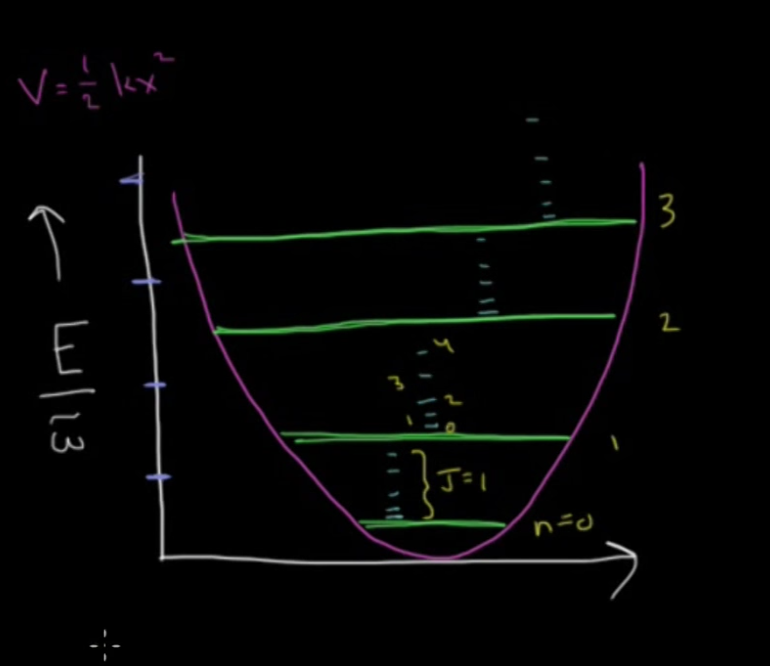
\includegraphics[width=0.75\textwidth]{figures/Screen Shot 2020-09-27 at 6.14.14 PM.png}
    \caption{Rovibrational energy diagram.}
    \label{fig:rovobo}
\end{figure}

\subsection{Spectrum of Rovibrational Transitions}

Our selection rules tell us that $\Delta n = +1$ for absorption, and we will also have $\Delta J = \pm 1$ when absorbing a photon. For us, this means that the frequency we observe will be:

\be
\tilde \omega_{obs} = \tilde E_{n+1, J+1} - \tilde E_{n, J}
\ee

We thus could have:

\be
\tilde \omega_{obs} = \tilde \omega + 2\tilde B \left(J+1\right), \text{ for } \Delta J = +1
\ee

or

\be
\tilde \omega_{obs} = \tilde \omega - 2\tilde B J, \text{ for } \Delta J = -1
\ee

In the spectrum, we thus have two different cases. The first $\Delta J = +1$ is called the R branch. This is higher in energy and thus frequency. For $\Delta J = -1$, this is the p-branch, has less energy, and thus lower frequency. We can then plot against frequency the type of spectrum we will see for rovibrations! 

 \begin{figure}
    \centering
    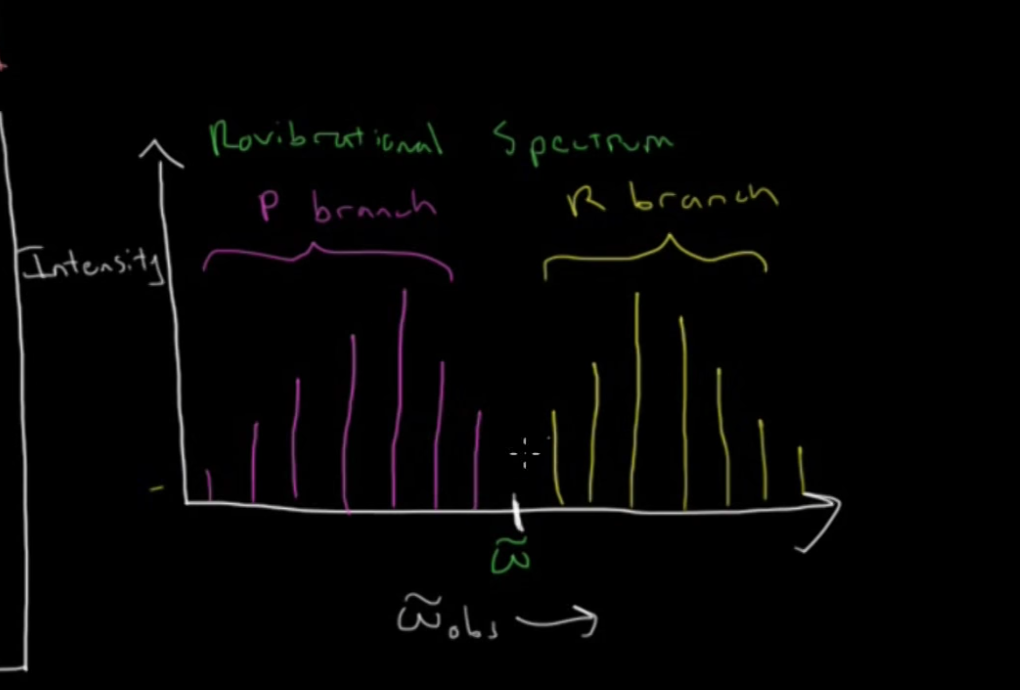
\includegraphics[width=0.75\textwidth]{figures/Screen Shot 2020-09-27 at 6.27.05 PM.png}
    \caption{Rovibrational spectrum.}
    \label{fig:rovospec}
\end{figure}

All of those peaks correspond to different starting $J$ levels outward from the center. The reason why the biggest branch is not the inner most is due to degeneracy ($2J+1$ degeneracy).

One last note:

\be
\Delta \tilde \omega_p > \Delta \tilde \omega_R
\ee

This is to say that the spacing between the bars are different. Why is the $p$ branch spacing larger? Check the next section...

\subsection{Rotation-Vibration Interaction}
 
Start above! Let's consider the potential energy $V(r)$. We can have some rotational energy levels that bounds. Let's look at the expectation value of $r$ (bond length). For a simple harmonic oscillator, these potentials are not symmetryic. It is stiffer on the small bond length side, and larger on the longer bond length size.

For a general state $n$, we have:

\be
\langle r \rangle_n > \langle r \rangle_0 
\ee

Because of this, we have an effect that modifies the energy levels of rotation as a function of vibrational energy level. Let's look at this in terms of $\tilde E_{n,J}$:

\be
\tilde E _{n,J} = \tilde \omega \left(n+\frac12\right) + \tilde B_n J \left(J+1\right)
\ee

We can rewrite this a bit:

\be
\tilde B_n = \tilde B_e - \tilde \alpha_e \left(n +\frac12\right)
\ee

where $\tilde \alpha_e$ is the \textbf{rotational-vibrational interaction constant}. This determines how much the bond lengthening at higher rotational levels affects our rotational constant. What does this mean for us? We can see that since, as $n$ increases, our bond length will increase slightly. As an effect, so does the moment of inertia. This causes our rotational constant $B$ to then decrease. What does this mean for our energy levels?

Consider the R branch and P branch:

\be
\tilde \omega_R = E_{1,J+1} - E_{0,J}
\ee

\be
\tilde \omega_R = E_{1,J-1} - E_{0,J}
\ee

What do these become?

\be
\tilde \omega_R = \tilde \omega + 2 \tilde B_1 + \left(3 \tilde B_1 - \tilde B_0\right)J + \left(\tilde B_1 - \tilde B_0\right)J^2
\ee

\be
\tilde \omega_P = \tilde \omega - \left(\tilde B_1 + \tilde B_0\right)J + \left(\tilde B_1 - \tilde B_0\right)J^2
\ee

We have identical quadratic terms in both the above expressions. Under the fully rigid rotor, this term goes away. Note also that it is a negative quadratic term since the difference out front is less than 0. 

So what does this actually all amount to?

As you increase $J$, this will be more and more negative. For the our branch, since these are increasing in frequency, will get closer together. The P branch on the other hand has decreasing frequency for increase in $J$, so the quadratic negative pushes them further apart. This is one reason why the P branch is more spread out than the R branch.

We can look at the linear term -- what is this telling us? The R branch linear prefactor is smaller than the prefactor for the P branch. Therefore the linear term again will drive R barnch together and P branch apart.

Note that this all goes away when you do not consider the rovibrational interaction (set $\alpha_e = 0$). 

I also note that $\tilde B_e$ and $\tilde \alpha_e$ have been tabulated by spectroscopists and you can look them up. 

\begin{figure}
    \centering
    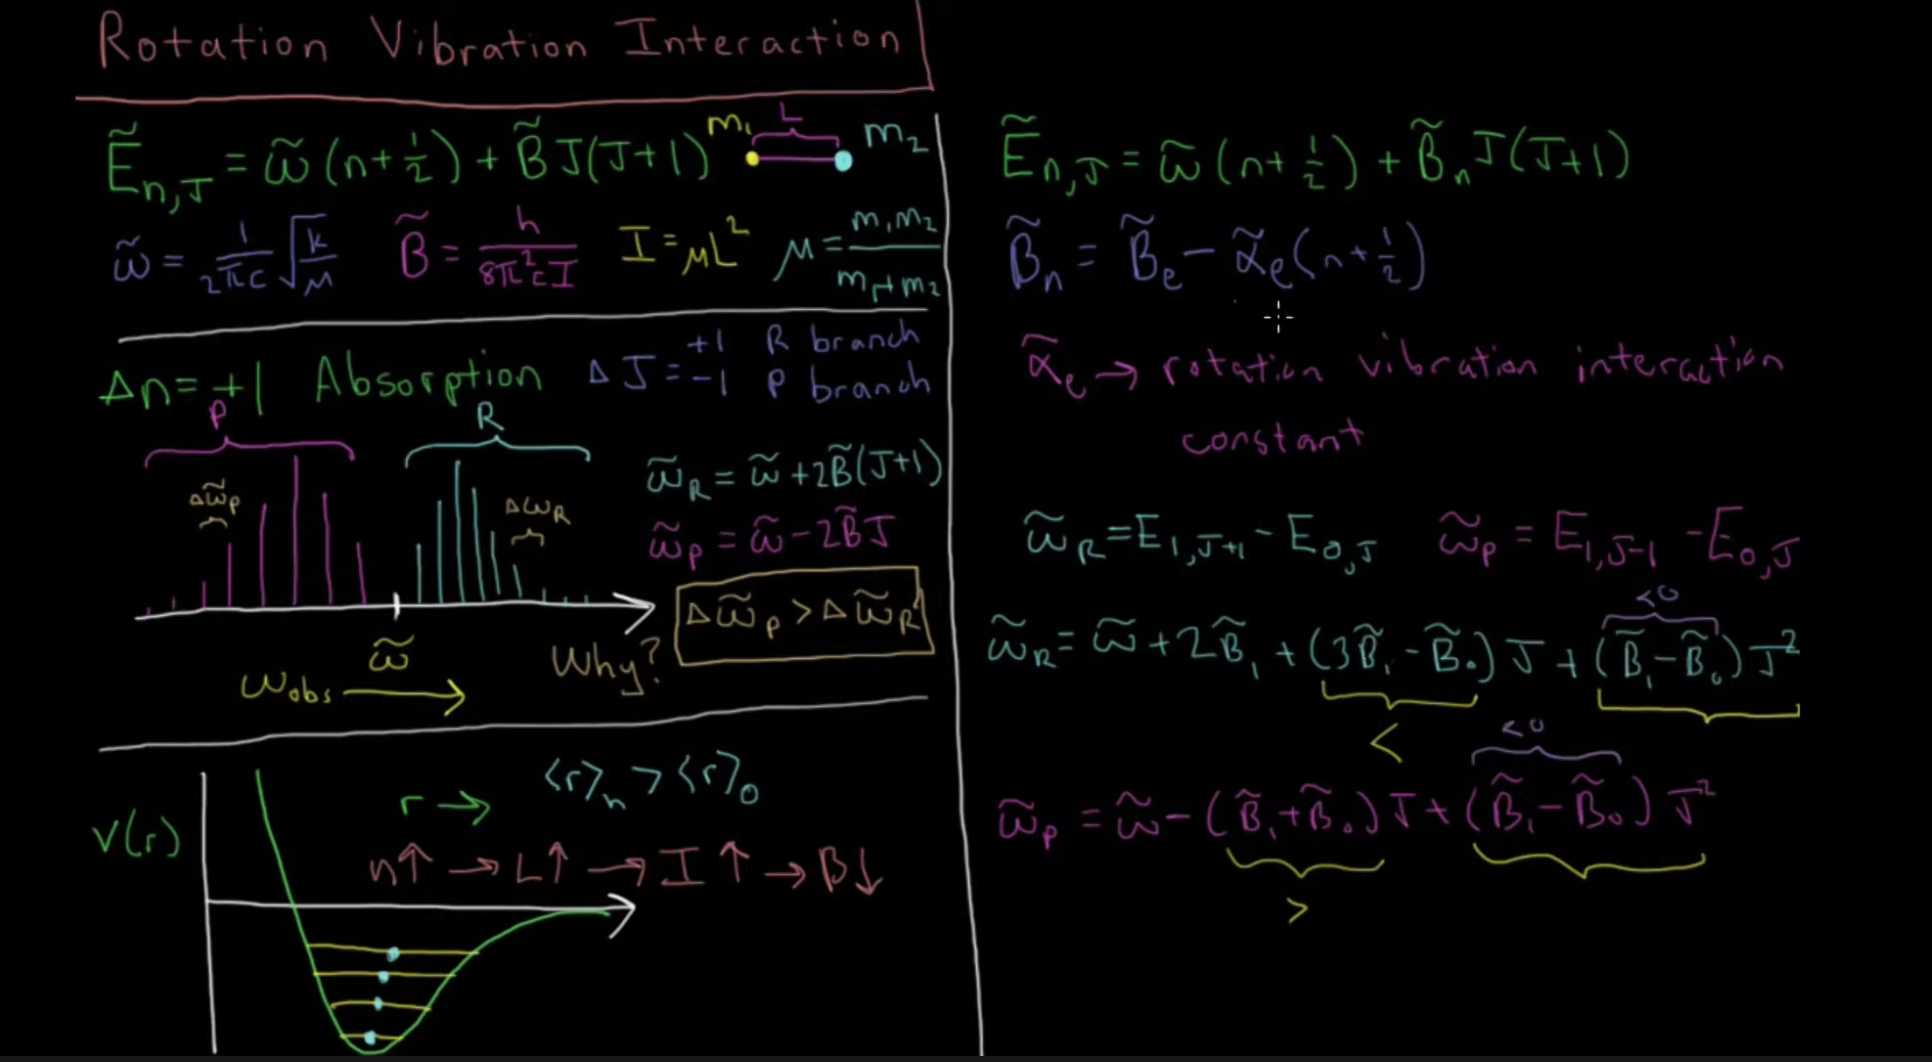
\includegraphics[width=0.75\textwidth]{figures/Screen Shot 2020-09-27 at 6.44.40 PM.png}
    \caption{Summary slide for this topic. }
    \label{fig:summ}
\end{figure}

\subsection{Order of Magnitude Energies}
The Born-Oppenheimer approximation allows us to treat the electrons in a molecule as a cloud-- they are much less massive and therefore have much higher velocities than the nuclei. If $L$ is the molecular size, typical electrons have momentum $\hbar /a$ and the electronic energy spacings can be expressed as:
$$ E_{elec} \sim \frac{\hbar^2}{mL^2}$$

\begin{figure}
    \centering
    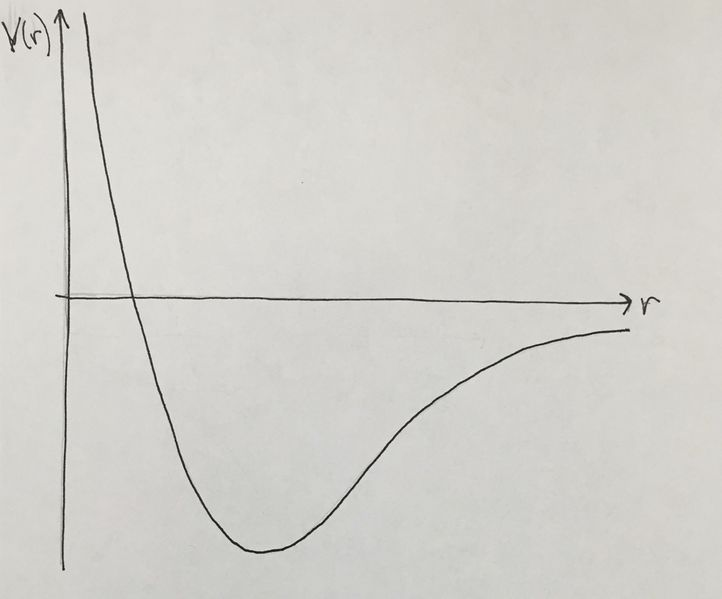
\includegraphics[width=0.75\textwidth]{figures/722px-Min.jpg}
    \caption{Internuclear potential}
    \label{fig:int_nuc_pot}
\end{figure}

The nuclei feel an equivalent potential that only depends on the internuclear distance and the electronic state. The internuclear potential has a minimum, and vibrations about the minimum can be roughly modeled as a harmonic oscillator. This potential is about $\frac{1}{2}M\omega^2 \xi^2$, where $\omega$ is the vibration frequency and $\xi$ is the displacement from equilibrium. If the displacement is the same order as the size of the molecule, the electronic energies should be about $\hbar^2 / 2mL^2$:

$$ \frac{1}{2} M \omega^2 L^2 \sim \frac{\hbar^2}{2mL^2} $$
$$E_{vib} \sim \hbar \omega \sim \left(\frac{m}{M}\right)^{1/2} \frac{\hbar^2}{mL^2} \sim \left(\frac{m}{M}\right)^{1/2} E_{elec} $$


The nuclei can also rotate, and have rotational energies that depend on their angular momentum. If $J$ is the quantum angular momentum number, 
$$ E_{rot} \sim \frac{\hbar^2 J (J+1)}{2I} $$
$$ I \sim M L^2 $$
For small $J$, 
$$ E_{rot} \sim \frac{m}{M} E_{elec} $$

So the electronic, vibrational, and rotational energy states have contributions that scale with the electron-to-nucleus mass ration:
$$ E_{elec} : E_{vib} : E_{rot} \sim 1: \left(\frac{m}{M}\right)^{1/2} : \left(\frac{m}{M}\right) $$


\subsection{Rotation-Vibration Spectra}

While it is possible to have a pure rotational spectrum, a pure vibrational spectrum is very unlikely: energies required to excite vibrations are much larger than those required to excite rotation. However, a combination of rotation and vibrational modes can be excited. 

Rotational energies can be described using the angular momentum number $J$:
$$E_{rot} = \frac{\hbar^2}{2I} J (J+1) $$

where $J = 0,\ 1,\ 2,\ ...$, $I$ is the moment of inertia, and $\mu$ is the reduced mass:
$$ I = \mu L^2 $$
$$ \mu = \frac{m_1 m_2}{m_1 + m_2} $$

The vibrations can again be modeled as a harmonic oscillator:
$$ E_{vib} = \hbar \omega (n + 1/2) $$
where $n = 0,\ 1,\ 2,\ ...$ and $\omega = \sqrt{k/m}$ where $k$ is the effective spring constant.

The total energy of rovibrational transitions, then, is:
$$ E_{rovibe} = \hbar \omega (n+1/2) + \frac{\hbar^2}{2I} J (J+1) $$

The selection rules for rovibrational transitions tell us that $\Delta n = +1$ and $\Delta J = \pm 1$. $\Delta J = +1$ is called the R branch, and $\Delta J = -1$ is called the P branch. This notation matches the videos above, but is {\bf opposite} the notation in Rybicki \& Lightman. We can use our rovibe energy expression to find the frequency of emitted photons for the R branch:
$$ \Delta J = +1 $$
$$ E_2 - E_1 = \hbar \omega (n+1 + 1/2) - \hbar \omega (n + 1/2) + \frac{\hbar^2}{2I} (J+1)(J+2) - \frac{\hbar^2}{2I} J (J+1) $$
$$ E_2 - E_1 = \hbar \omega + \frac{\hbar^2}{I} (J+1) = \hbar \omega_{obs, R} $$
$$ \omega_{obs, R} = \omega + \frac{\hbar}{I} (J+1) $$

and the P branch:
$$ \Delta J = -1 $$
$$ E_2 - E_1 = \hbar \omega (n+1 + 1/2) - \hbar \omega (n + 1/2) + \frac{\hbar^2}{2I} (J-1)(J) - \frac{\hbar^2}{2I} J (J+1) $$
$$ E_2 - E_1 = \hbar \omega - \frac{\hbar^2}{I} J = \hbar \omega_{obs, P} $$
$$ \omega_{obs, P} = \omega - \frac{\hbar}{I} J $$


\begin{figure}[ht]
    \centering
    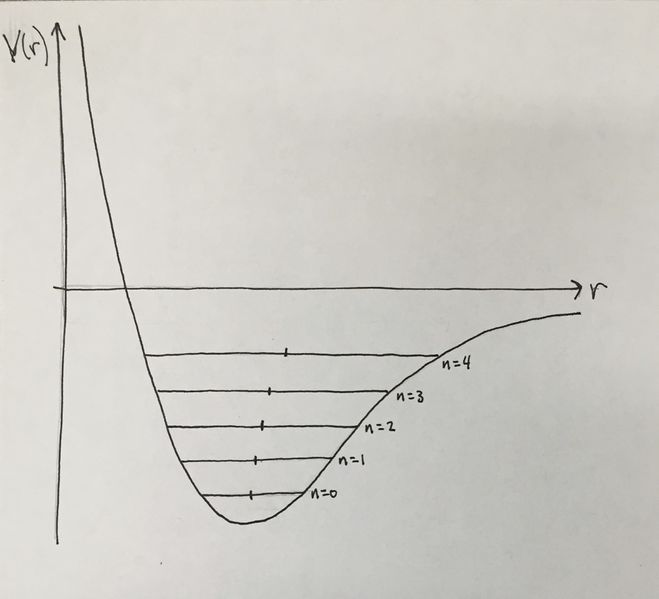
\includegraphics[width=0.75\textwidth]{figures/659px-Asymm.jpg}
    \caption{Asymmetries in the potential: note that bond length increases with increasing n.}
    \label{fig:asymm}
\end{figure}


However, we should note that the potential is {\it not} perfectly harmonic; the slight asymmetries we can see in the potential cause the bond length to increase as $n$ increases. So if $n$ increases, $L$ increases, causing $I$ to increase. Our rovibrational energy expression depends on $I^{-1}$, so the energy {\it decreases} as $n$ increases. This effectively pulls all of our spectral lines to the left, which decreases the separation between lines on the R branch and increases the separation between lines on the P branch. Similar effects can also be found when comparing the expressions for the observed frequencies. Putting everything together, we can plot our rovibrational spectrum.

\begin{figure}[ht]
    \centering
    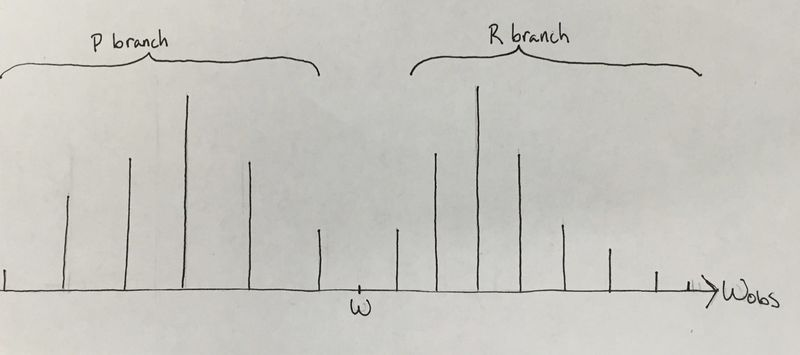
\includegraphics[width=0.75\textwidth]{figures/800px-Spectrum.jpg}
    \caption{Rovibrational spectrum}
    \label{fig:rovooooospec}
\end{figure}


\subsection{Class Notes}

Let's now talk about the previous content together! Vibrational transitions cannot happen by themselves since photons must carry angular momentum. You can't create this without changing $L$ state. You \textbf{must} do a rotational transition at the same time when you do a vibrational transition. 

Vibrational transitions are almost always more energetic than rotational transitions, by the way. Vibrational are around $30-1000\times$ more energetic, BUT the rotational \textit{can} be a significant decrement of the total transition  so we think of them together. 

Let's talk really quickly about the $P$ and $R$ branch spacing one more time before the activity:

Suppose we have an atom that can both rotate or vibrate. We know the vibrational energies are much larger than the rotational energies. The rotational states have quadratic spacing between TWO vibrational states. We can jump between different points on these ladders, ensuring that we fulfill the selection rules. For the basic strong transitions, $J$ must change by $\pm 1$. If you start in both the ground rotational and vibrational states. You cannot jump to ground state of the vibrational transitions since we must change $J$. This is ``forbidden.'' 

The energy spacing from $n= 0 \rightarrow n =1$. You won't see a line at this $\Delta E$ since you cannot go straight into there. What can you do? You can go to the $J=1$ state AND the $n=0 \rightarrow n = 1$ state. The energy of the jump will be HIGHER than the average $\Delta n$ change. This pushes the line to higher energy. We can do this with the whole comb of transitions. Take a look at this diagram:

\begin{figure}
    \centering
    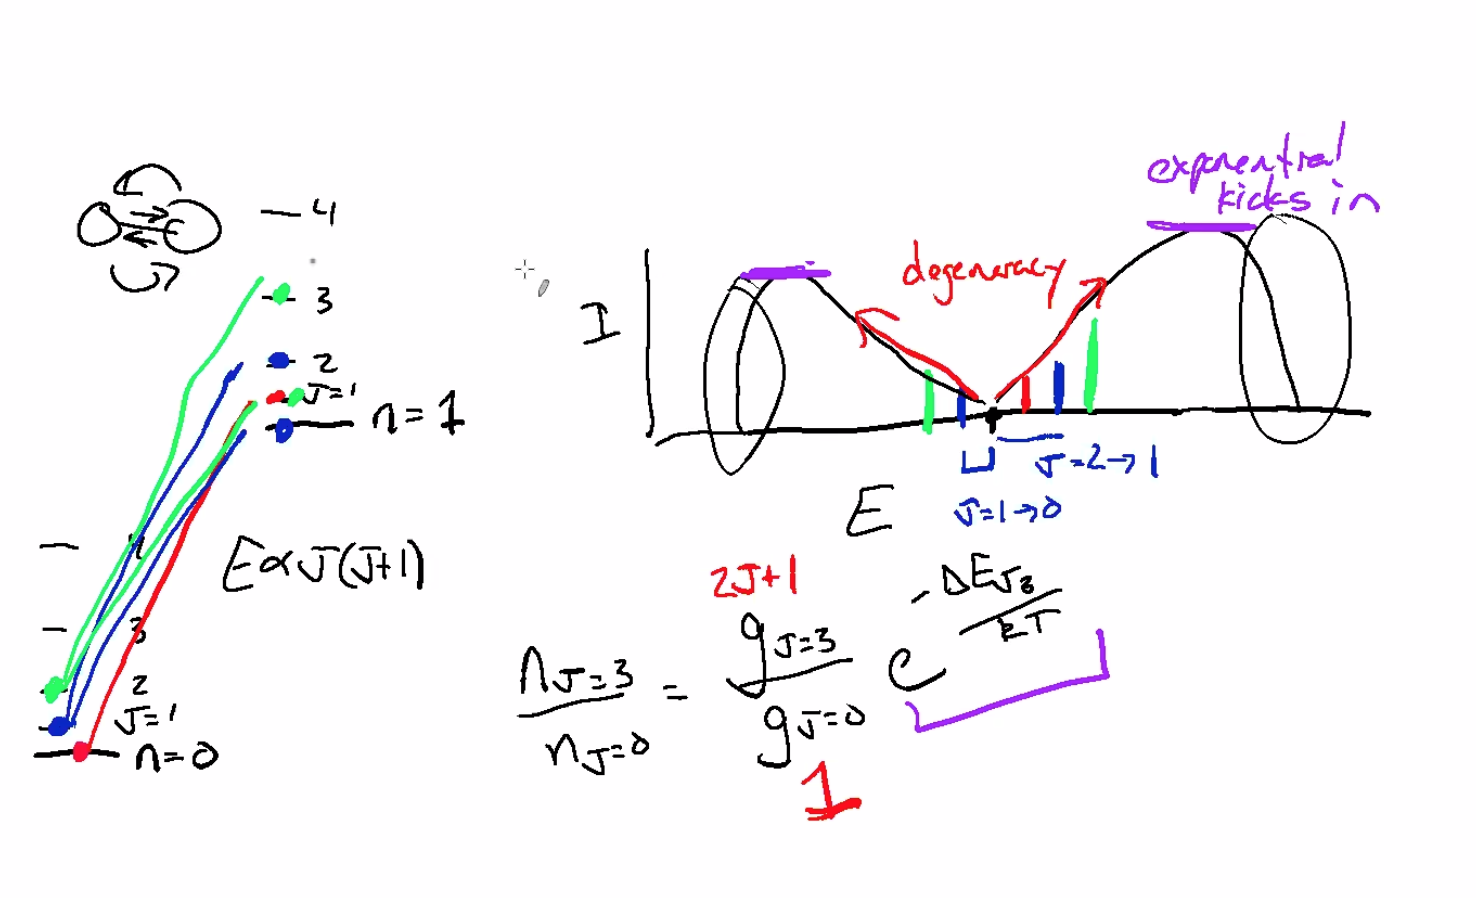
\includegraphics[width=0.75\textwidth]{figures/Screen Shot 2020-10-01 at 11.29.37 AM.png}
    \caption{P and R branch source. This answers whether or not the transitions are taking energy away or adding to the vibrational transitions. The gap in the middle is because we do not see the direct vibrational transition without the change in rotation. Why should it start falling off, though? Think the Boltzmann equation -- it takes energy to be in a rotational state. How much energy did we have floating around in this atom? The more energy we hold, the harder it is to source from the ambient energy. If $kT$ is really high, the thing that sets the slope is the degeneracy! At the flat part, we start to feel the exponential cutting us off. }
    \label{fig:ro_explanation}
\end{figure}

Some others notes that are interesting: atomic Hydrogen clouds are cold, but not as cold as the background. Atomic hydrogen is not found where star formation is happening. If you don't cool down these clouds, the clouds will be held up by collisional pressure, preventing the collapse of these clouds. We require cooling to collapse to a star. Also, as you collapse, you keep heating, so you have to keep cooling! {\textbf If you cannot cool effectively, you cannot form structure.}

Most of the mass of these clouds is molecule hydrogen $H_2$. This is not to be confused with HII which is singly ionized Hydrogen (a proton). So how do we cool molecular hydrogen?

%%%%%%%%%%%%%%%%%%%%%%%%%%%%%%%%%%%%%%%%%%%%%%%%%%%%%%%%%%%%%%%%%%%%%%%%%%%%%%
%%%%%%%%%%%%%%%%%%%%%%%%%%%%%%%%%%%%%%%%%%%%%%%%%%%%%%%%%%%%%%%%%%%%%%%%%%%%%%
%%%%%%%%%%%%%%%%%%%%%%%%%%%%%%%%%%%%%%%%%%%%%%%%%%%%%%%%%%%%%%%%%%%%%%%%%%%%%%
\newpage
\section{October 6, 2020: MASERs}

\subsection{Video Notes}

MASERs are just lasers at low frequency! We need to know a few things to understand them -- consider a photon being absorbed by an electron, sending the electron from the $n = 1 \rightarrow 2$ state. After absorption, the electron emits a photon and slides back down to the ground state. This is spontaeous emission. Normally, the time it takes is around $10^{-8} \s$. There are states that are called ``meta-stable'' which are much longer lived ($10^{-3} \s$). These meta stable states are essential for MASERs.

Stimulated emission happens when a photon interacts with an electron, cause it to emit a photon that is coherent and in phase with the original photon. If we have a series of these stimulated emission processes, we can very rapidly collect coherent, in-phase and extremely focused. 

These can be incredibly bright when powered by stimulated emission, with brightness temperature around $10^{14} \K$. 

Consider a slab of molecules, distributed homogeneously in the slab. There are two energy levels, $E_1$ and $E_2$. We have the intensity:

\be
I_\nu = S_\nu \left(1 - e^{-\tau_\nu}\right)
\ee

where 

\be
S_\nu = \frac{\overbrace{n_2 A_{21} h \nu \phi(\nu) \frac{1}{4\pi}}^{j_\nu} }{
\underbrace{
\frac{h \nu}{4 \pi} \phi(\nu)\left(\underbrace{n_1 B_{12}}_\text{absorption} - \underbrace{n_2 B_{21}}_\text{stimulated emission}\right)
}_{\alpha_\nu}
}
\ee

Now remember:

\be
g_1 B_{12} = g_2 B_{21} 
\ee

and 

\be
\frac{\ato}{\bto} = \frac{2 h \nu^3}{c^2}
\ee

And we end up with:

\be
S_\nu = \frac{2 h \nu^3}{c^2} \frac{1}{\frac{n_1 g_2 }{g_2 g_1} - 1}
\ee

In this derivation, we assumed that we had a population inversion. But how do we get a population inversion? We cannot get that in a 2-state system because of the {\textbf Principle of Detailed Balance}. In a three state system, though, we can have a fast de-excitation from say the $n = 3 \rightarrow 2$ state, and a slow $n = 2 \rightarrow 1$ transition. This gives us a consistent population inversion. This keeps lots of atoms in the $n=2 $ state. Now we can have a maser! In nature, we usually see 4-state MASER systems, behaving similar but with an extra level. 

If $\frac{n_1}{g_1} < \frac{n_2}{g_2} \rightarrow S_\nu < 0 $ which is really weird. Additionally, the optical depth $\tau_\nu$ is weird:

\be
\tau_\nu = \alpha_\nu L = \frac{h \nu}{4 \pi} \phi(\nu) \bto \left(\frac{n_1 g_2}{g_1} - n_2\right) L
\ee

\be
\tau_\nu = \frac{h \nu}{4 \pi} \phi(\nu) \bto n_2 \left(\frac{n_1 g_2 }{g_2 n_1} - 1\right)L
\ee

Here, we see again that if $n_1 g_2 < n_2 g_1$, then we have negative optical depth which is really strange! This seems like it is breaking down, but optical depth and the source function are NOT observables. We care that the specific intensity is still positive, and we have:

\be
I_\nu = S_\nu \left(1 - e^{-\tau_\nu}\right)
\ee

Thus, if $\tau_\nu$ is negative, and if $\tau \ll 1$, then we have that $I_\nu = S_\nu \tau_\nu$, and the product of two negatives is a positive, so we're okay. Additionally, if $\tau_\nu \ll -1$, then we have $I_\nu \gg 1$.


\subsection{ Cosmic Masers }

$OH$ and $H_20$ masers can occur in dusty, star-forming regions which are cold
enough for these molecules to form.  The dust's black-body radiation in
the infrared band is absorbed by these molecules and a population
inversion is established.  When maser emission is caused by via stimulated
emission, these clouds can get very bright (brightness temperatures $\sim
10^{14}K$).  Temperatures this high cannot be thermal, so we know a maser
when we see one. \par
Generally, masers are useful for tracing the galaxy's magnetic field (emission
lines are Zeeman split), and for following disks of gas and dust around stars
in star-forming regions.  In order to detect them, we need clouds which are
moving uniformly together, and have velocity coherence both $\perp, \|$ to
our line-of-sight through a disk of rotation gas.  
In general, the intensity we observe depends on the
path length through the masing cloud, so we like long path lengths with the
same velocity.

\subsection{ How Masers Work }
We will discuss population inversion a bit later, for now lets just assume that there are many more atoms in state 2 then state 1, where state 2 has higher energy than state 1. If a photon with an energy equal to E2-E1 comes along and interacts with an atom, it will thus be significantly more likely to produce stimulated emission (i.e., cause the atom to emit an identical photon with energy E2-E1 and drop from state 2 to 1) than to radiatively excite the atom (i.e., absorb the photon and transition from state 1 to 2). We will ignore the possibility of radiative excitation from state 1 to 2 entirely. The duplicate pair of photons produced by stimulated emission then go on to interact with other atoms leading to an exponential increase in the number of photons (and thus the intensity of radiation). 
Now onto the math.

Consider a molecule with two rotational energy levels.  Observing a homogeneous
slab of this molecule, the intensity we receive is given by the familiar:
$$I_\nu=S_\nu(1-e^{-\tau_\nu})$$
where $S_\nu=\frac{j_\nu}{\alpha_\nu}$.  $j_\nu$ and $\alpha_\nu$ are given by:
$$\begin{aligned}j_\nu&=\overbrace{n_2\ato}^{per time}\overbrace{h\nu}^{per E}
\overbrace{\phi(\nu)}^{per\ Hz}\overbrace{\inv{4\pi}}^{per steradian}\\ 
\alpha_\nu&=\frac{h\nu}{4\pi}\phi(\nu)[\overbrace{n_1\bot}^{abs}-\overbrace{
n_2\bto}^{stim emis}]\\ \end{aligned}$$
Thus, our source function looks like:
$$S_\nu=\frac{n_2\ato\phi(\nu)h\nu\inv{4\pi}}{\frac{h\nu}{4\pi}\phi(\nu)[n_1\bot-
n_2\bto]}$$
Then since $g_1\bot=g_2\bto$ and $\frac{\ato}{\bto}=\frac{2h\nu^3}{ c^2}$, we have:
$$S_\nu=\frac{2h\nu^3}{ c^2}\inv{\frac{n_1g_2}{ g_1n_2}-1}$$
A population is said to be inverted when $n_1g_2<g_1n_2$ (not $n_1<n_2$).
$\frac{n_1}{ g_1}$ is an expression for the population per degenerate sub-level in
energy level 1.  If $\frac{n_1}{ g_1}<\frac{n_2}{ g_2}$, then $S_\nu<0$, and we
have a maser.  Expressed in terms of the excitation temperature ($\frac{n_2}{ n_1}
=\frac{g_2}{ g_1}e^{-\frac{h\nu}{ kT_{ex}}}$), we have:
$$S_\nu=\frac{2h\nu^3}{ c^2}\inv{e^\frac{h\nu}{ kT_{ex}}-1}$$
which is less than 0 when $T_{ex}<0$.  We can express the optical depth of
this slab to maser radiation as:
$$\tau_\nu=\alpha_\nu L
=\frac{h\nu}{4\pi}\phi(\nu)\bto\left[\frac{n_1g_2}{g_1}-n_2\right] L
=\frac{h\nu}{4\pi}\phi(\nu)\bto n_2\left[\frac{n_1g_2}{ g_1n_2}-1\right] L$$
If $\frac{n_2}{ g_2}>\frac{n_1}{g_1}$, then $\tau_\nu<0$.  Now you might think
we're talking nonsense with a negative source function and a negative optical
depth, but we're not. Only observable quantities need to be positive, since optical depth and the source function are just mathematical record keeping objects,
they can take on any values.
  Recall that the intensity is:
$$I_\nu=S_\nu(1-e^{-\tau})$$
If $\tau\to-\infty$, then $I_\nu\to-S_\nu e^{\tau_\nu}$, so $I_\nu\gg1$. 
On the other hand, if $\tau<0$ and $|\tau|\ll1$, then $I_\nu\to S_\nu\tau_\nu$,
which is the product of two negatives = positive.  This should be convincing
you that $I_\nu$ is always positive, and therefore, actually manifested.

\subsection{ Maser Species }

$OH$ mases at around 18 cm, and is found around AGB (asymptotic-giant-branch)
stars in star-forming regions and around the galactic nucleus.  AGB's are
important because they have lots of dust.  The two masing transitions are
from $1667\to1612MHz$ and $1720\to1665MHz$.\par
$H_2O$ mases at $1.35 cm$ in a transition to its ground rotational state.  Note
that an order-of-magnitude calculation of $\Delta E=\frac{\hbar}{ 2I}$ for $H_2O$
gives us an estimate of $\sim 1 mm$, which is incorrect.  The correct 
transitional energy is caused by a slight degeneracy in water molecules.\par
$SiO$ mases at $3.4 mm$ in its ground vibrational state, and is typically
found in star-forming regions and around AGB stars.\par
Other molecules mase, and there is even potential for detecting atomic lasers 
around massive stars ($L\sim10^5 L_\odot$).  Hydrogen transitions from $10\to9$
have been observed (at $55\mu m$), and Stielnitski 1996 claims to have observed
a population inversion in atomic H.

\subsection{ Saturated vs. Unsaturated masers }

There are two modes of operation for masers.  For unsaturated masers, the gain
is exponential with the path length, and for saturated ones, the gain only
grows linearly with path length.  The masers we find in the cosmos are typically
saturated.  The following is working toward understanding why there are two
modes in masers. Before we start with the math lets imagine a sequence of events that
might lead to saturation. Initially we have lots of atoms in state 2. If a photon that has
energy E2-E1 interacts with one of these atoms we get two identical photons. Both of these photons
can then interact with other atoms in state 2 giving 4 photons. This leads to an exponential amplification
of the number of photons. If this increasing number of photons continues to propogate through the atoms, a point will eventually be reached where 
there are more photons with energy E2-E1 then there are atoms in state 2 for them to interact with. This means that we transition from an exponential amplification
(from photon doubling) to a linear amplification (from continuing to travel through a medium with some density of atoms in state 2). This is called saturation.
The graph given below shows intensity $I_\nu$ as a function of optical depth $\tau$. The discontinuity in the derivative on the graph is the saturation point.

\begin{figure}
    \centering
    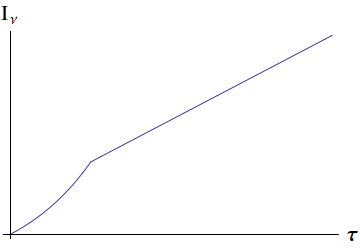
\includegraphics[width=0.75\textwidth]{figures/MaserIntensity.png}
    \caption{Maser Intensity}
    \label{fig:maserintensity}
\end{figure}

Now let us prove this intuitive solution mathematically.
  We begin with the expression for specific intensity from
emissivity (see Radiative Transfer Equation and Einstein Coefficients):
$$\begin{aligned}\frac{dI_\nu}{ dz}&=j_\nu-\alpha_\nu I_\nu\\ 
&=\frac{h\nu}{4\pi}\phi(\nu)n_2A_{21}-\frac{h\nu}{4\pi}
\phi(\nu)[n_1\bot-n_2\bto]I_\nu\\ \end{aligned}$$
In principle, the Line Profile Functions governing spontaneous emission and the
line-profile governing stimulated emission might not have to be the same, but
evidence seems to suggest they are.  Let's assume they are, and rewrite this:
$$\begin{aligned}\frac{dI_\nu}{ dz}&=\frac{h\nu}{4\pi}\phi(\nu)\frac{n_2\ato}{ g_2}\cdot g_2
-\frac{h\nu}{4\pi}\phi(\nu)g_2\bto\left[\frac{n_1}{ g_1}-\frac{n_2}{ g_2}\right]
\end{aligned}$$
Defining $N_1\equiv\frac{n_1}{ g_1}$, $N_2\equiv\frac{n_2}{ g_2}$, $A\equiv
\ato g_2$, and $B=\bto g_2$, our equation looks like:
$$\frac{dI_\nu}{ dz}=\frac{h\nu}{4\pi}\phi(\nu)[N_2A+B(N_2-N_1)I_\nu]$$
Now we'll integrate over frequency.  $\phi(\nu)$ is a sharply peaked function,
so we'll treat it as a $\delta$-function.  Then substituting
$I\equiv\int{\phi(\nu)I_\nu d\nu}$, we have:
$$\frac{\int{I_\nu d\nu}}{\Delta\nu}\equiv\int{I_\nu\phi(\nu)d\nu}$$
which is true by definition of $\Delta\nu$: $\int{I_\nu d\nu}=I\Delta\nu$.
So now we have:
$$\frac{dI}{ dz}=\frac{h\nu}{4\pi\Delta\nu}[(N_2-N_1)BI+N_2A]$$
This is an equation with three unknowns.  To close this system, we'll use the
equations of statistical equilibrium, which say:
$$\frac{dN_2}{ dt}=-N_2BJ+N_1BJ-N_2A+R_2(N-N_1-N_2)-\Gamma_2N_2$$
where $J\equiv\int{I_\nu\phi(\nu)d\nu}$, and $J_\nu=\inv{4\pi}\int{I_\nu
d\Omega}$.  $R_2$ is the ``pumping rate''.  It describes the rate at which
molecules not in state 1 or 2 (counted by $N-N_1-N_2$) are radiatively or 
collisionally
knocked into state 2. $\Gamma_2$ is the loss rate of molecules in state 2 into
any state other than state 1.  In the above equation, we've neglected two
terms: collisional excitation $1\to2$ and $2\to1$.  These are crucial terms,
being tightly related to local thermal equilibrium.  However, we will neglect
them to simplify analysis.  We also have a similar equation for state 1:
$$\frac{dN_1}{ dt}=N_2BJ-N_1BJ+N_2A+R_1(N-N_1-N_2)-\Gamma_1N_1$$
We'll further simply matters by setting the loss-rates for the two populations
equal to each other ($\Gamma_1=\Gamma_2=\Gamma$).  Now let's solve for the 
steady-state solution ($\frac{dN}{dt}=0$).
$$\frac{d(N_2-N_1)}{ dt}=-(N_2-N_1)2BJ-2N_2A+(R_2-R_1)(N-N_{12})-\Gamma(N_2-N_1)$$
where $N_{12}=N_1+N_2$.
Two terms in this equation are acting to reduce the population inversion of
state 2 with respect to state 1: $(N_1-N_1)2BJ$ and $\Gamma(N_2-N_1)$.  In the
{\it unsaturated regime} where $BJ\ll\Gamma$, stimulated emission is a minor
perturbation to the inverse.  In this case we can solve the system of equations:
$$\begin{aligned}\frac{d\Delta N}{dt}=\frac{d(N_2-N_1)}{ dt}&=-2N_2A+(R_2-R_1)(N-N_{12})
-\Gamma\Delta N=0\\ 
\frac{dN_{12}}{ dt}&=(R_2+R_1)(N-N_{12})-\Gamma(N_1+N_2)=0\\ \end{aligned}$$
Then solving for $N-N_{12}$:
$$N-N_{12}=\frac{\Gamma(N_1+N_2)}{ R_1+R_2}=\frac{\Gamma N_{12}}{ R_1+R_2}$$
Substituting this into the difference equation, which reads:
$$-2N_2A=\frac{R_2-R_1}{ R_1+R_2}\Gamma N_{12}-\Gamma\Delta N=0$$
the using $N_2=\frac{N_{12}+\Delta N}{2}$ (this is just an identity), we get:
$$\underbrace{\left(1+\frac{\Gamma}{ A}\right)}_{\equiv2\beta}\Delta N
=N_{12}\left[\underbrace{\frac{R_2-R_1}{ R_1+R_2}\frac{\Gamma}{ A}}_{\equiv
\inv{\alpha}}-1\right]$$
Thus:
$$\Delta N=\frac{N_{12}}{2\beta}\left[\inv{\alpha}-1\right]=\frac{N_{12}(1-\alpha)}{
1\alpha\beta}$$
Now we'll define $S\equiv\frac{\alpha\beta}{1-\alpha}$.  $S$ is meant to connote
the source function here.  The reason we might expect $S$ to be related to
the source function is that $S_\nu\propto\frac{N_2}{N_2-N_1}\propto\frac{N_2}{
\Delta N}$, so $\Delta N\propto \frac{N_{12}}{2S}$.  This is why we use an $S$
here.  Getting back to our original equation, we have:
$$\frac{4\pi\Delta\nu}{ h\nu A}\frac{dI}{dz}=\Delta N\underbrace{\frac{BI}{A}}_{
\equiv\mathfrak{I}}+N_2$$
Using our newly defined $S$, this becomes:
$$\frac{4\pi\Delta\nu}{ h\nu B}\frac{d\mathfrak{I}}{dz}=\frac{N_{12}}{2S}\mathfrak{I}+
\hf(N_{12}+\Delta N)$$
Finally, defining an unsaturated gain length $L\equiv\frac{4\pi\Delta\nu}{ Bh\nu}
\frac{2S}{N_{12}}$, we have:
$$L=\mathfrak{I}+S+\hf$$
Then using $ds=\frac{dz}{ L}$, we have:
$$\frac{d\mathfrak{I}}{ds}=\mathfrak{I}+\hf+S$$


To order of magnitude:
$$\begin{aligned}\mathfrak{I}&\equiv\frac{B}{A}I=\frac{B}{ A}B_\nu(T_{bright})\\ 
&=\frac{c^2}{2h\nu^3}\frac{2h\nu^3}{ c^2}\inv{e^\frac{h\nu}{ kT_{bright}}-1}\\ 
&=\inv{e^\frac{h\nu}{ kT_{bright}}-1}\\ \end{aligned}$$
Now since $1\ll\frac{kT_{bright}}{h\nu}$ (typical maser wavelengths are in
mm and $T_{bright}$ is typically several K), we can throw away our $\hf$ in
our equation for $\frac{d\mathfrak{I}}{ds}$:
$$\frac{d\mathfrak{I}}{ds}=\mathfrak{I}+S\Rightarrow
\int\frac{d\mathfrak{I}}{\mathfrak{I}+S}=\int{ds}\Rightarrow
\mathfrak{I}+S=De^s$$
Choosing $\mathfrak{I}=0, s=0$ (we're assuming there is no background source), then
$D=S$, so:
$$\boxed{\mathfrak{I}=S(e^s-1)}$$
If $s\ll1$, we have $\mathfrak{I}=Ss$ from spontaneous emission, and this is the 
saturated case.  If $s\gg1$, the $\mathfrak{I}=Se^s$ from stimulated emission, and
this is the unsaturated case.  Earlier we threw away the $BJ$ term, but we
could have done all of this including that term, and the algebra would have
been the same.  If we do this, we get the answer:
$$\boxed{\frac{d\mathfrak{I}}{ ds}=\frac{\beta(\mathfrak{I}+\hf)}{\beta+\mathfrak{J}}+S}$$
where $\mathfrak{J}$ is the non-dimensionalized, integrated flux, 
$\mathfrak{J}=\frac{BJ}{ A}$.

\subsection{ The Saturated Mode }

Recall our masing equation:
$$\frac{d\mathfrak{I}}{ ds}=\frac{\beta(\mathfrak{I}+\hf)}{\beta+\mathfrak{J}}+S$$
In the unsaturated case, $\frac{\beta}{\beta+\mathfrak{J}}\to1\iff\beta\gg\mathfrak{J}$.
This is equivalent to saying:
$$\hf\left(1+\frac{\Gamma}{ A}\right)\gg\frac{BJ}{ A}$$
And if $\Gamma\gg A$, then:
$$A+\Gamma\gg BJ\iff\Gamma\gg BJ$$
In the saturated case, then $\beta\ll\mathfrak{J}$.  In this case:
$$\frac{d\mathfrak{I}}{ds}=\frac{\beta\mathfrak{I}}{\mathfrak{J}}+S=\frac{4\pi\beta\mathfrak{I}}{
\int{\mathfrak{I}ds}}+S$$
where we used that $\mathfrak{J}\sim\inv{4\pi}\int{\mathfrak{I}d\Omega}$.  If we consider
a single beam of photons through a cloud, then $\int{\mathfrak{I}d\Omega}\approx
\mathfrak{I}\Delta\Omega$, so:
$$\boxed{
\begin{aligned}\frac{d\mathfrak{I}}{ ds}&=\frac{4\pi\beta\mathfrak{I}}{\mathfrak{I}\Delta\Omega}+S\\ 
&=\frac{4\pi\beta}{\Delta\Omega}+S\\ \end{aligned}}$$

\subsection{ How We Get Population Inversions }

\begin{figure}
    \centering
    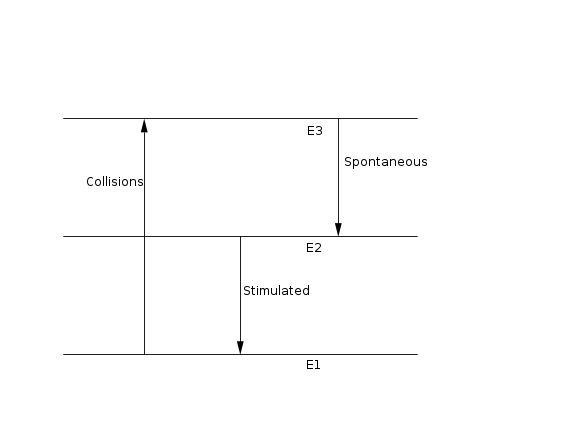
\includegraphics[width=0.75\textwidth]{figures/Atom.png}
    \caption{Atom.}
    \label{fig:atom}
\end{figure}

There is another dichotomy in masers: ones which are excited radiatively and
those which are excited collisionally.  We'll discuss a cloud of molecules
which have 3 energy states which are populated by {\it simple collisional
pumping}. Before we dive into the math lets consider conceptually what is going on.
The diagram shows a simple 3 state atom. We can only go between state E1 and E3 collisionally (ie they do not communicate radiatively).
State E3 spontaneously decays radiatively to state E2 with a short lifetime. State E2 radiatively decays to state E1, but with a very long lifetime.
This means that there can be a large number of atoms that are in state E2. Thus we have the requisite population inversion for masing to occur.
Now onto the math.
  The rate of change of the population of energy state
1 in this case is given by (sources - sinks):
$$\frac{dn_1}{ dt}=n_2\ato+n_2C_{21}+n_3C_{31}+n_2\bto J_{21}-n_1\bot J_{12}
-n_1C_{12}-n_1C_{13}$$
Then $J_{12}=J_{21}$, and because of local collisional thermal equilibrium,
$C_{12}=C_{21}\frac{g_2}{ g_1}e^{-{E_{21}}{ kT}}$.  Similarly,
$C_{13}=C_{31}\frac{g_3}{ g_1}e^{-{E_{21}}{ kT}}$.  So dividing by $g$, and
defining $N_1\equiv\frac{n_1}{ g_1}$, we have:
$$\begin{aligned}\frac{dN_1}{ dt}=&\underbrace{\frac{n_2}{ g_2}}_{N_2}\underbrace{
\frac{\ato}{ g_1}g_2}_{\ato}+\underbrace{\frac{n_2}{ g_2}}_{N_2}\underbrace{
\frac{C_{21}}{ g_1}g_2}_{\equiv C}+\underbrace{\frac{n_2}{ g_3}}_{N_3}\underbrace{
\frac{C_{31}}{ g_1}g_3}_{\equiv C}+\underbrace{\frac{n_2}{ g_2}}_{N_2}\underbrace{
\frac{\bto}{ g_1}g_2}_{\bto}J_{21}\\
&-N_1\underbrace{\bto}_{\bto\frac{g_2}{ g_1}\equiv
\bto}-N_1\underbrace{C_{21}\frac{g_2}{ g_1}}_{\equiv C}e^{-\frac{E_{21}}{ kt}}-
N_1\underbrace{C_{31}\frac{g_3}{ g_1}}_{\equiv C}e^{-\frac{E_{31}}{ kT}}\\
\end{aligned}$$
Phew.  Notice that we set $C_{21}=C_{31}$.  This is just to make our lives
easier.  We can do the same for $\frac{dN_2}{ dt}$, but omitting $B_{23}$, because
we're deciding not to have absorptions from $2\to3$ and no stimulated emission
from $3\to2$.  Then our total population is $N=N_1+N_2+N_3$.  Without being
careful, instinct tells us that in steady state, we'll have a population
inversion $\frac{N_2}{ N_1}>1$ if $C\ll A_{32}$.  This
instinct is correct, but let's do this carefully.  First we'll make some
assumptions:
\begin{itemize}\item $\ato\ll C$.  For $H_2O$: 
$$\ato\sim10^8s^{-1}\left(\frac{1216\angstrom}{1.35cm}\right)^3
\sim10^8\e{-15}s^{-1}
\sim10^{-7}s^{-1}\left(\frac{\mu}{ ea_0}\right)^2$$
where $\mu$ is our way of accommodating the fact that the dipole moment for
$H_2O$ might not be the same as for the fine structure of hydrogen.  It turns
out the answer is $\ato\sim2\e{-9}s^{-1}$.\par
Estimating C:
$$C\sim n_{H_2}\sigma v_{rel}\sim n_{H_2}\e{-15}\cdot(3\frac{km}{ s})
\sim n_{H_2}\cdot3\e{-10}$$
which is $\gg10^{-7}s^{-1}\left({\mu}{ ea_0}\right)^2$ when
$n_{H_2}\gg10^3cm^{-3}\left(\frac{\mu}{ ea_0}\right)^2$.  
\item Next we'll assume $E_{21}\ll kT$.  Define $\frac{E_{21}}{ kT}\equiv\delta
\ll1$.\end{itemize}
Now we have a 2-step:
\begin{itemize}\item Step 1: Since $1\to3$ are not linked by radiation,
$$\frac{N_3}{ N_1}\approx e^{-\frac{E_{31}}{ kT}}\equiv\theta\le1$$
\item Step 2: Radiative decays from $3\to2$.  To get an inversion, we'll
argue that the sources into 2 are larger than the sinks out of 2 (this is 
a little weird because we're solving our steady-state equations, but whatever):
$$N_3A_{32}+N_3C+N_1Ce^{-\frac{E_{21}}{ kT}}>N_2Ce^{-\frac{E_{32}}{ kT}}+N_2C$$
We can rewrite this as:
$$\begin{aligned}
\underbrace{\frac{N_2}{ N_1}}_{=\theta}\frac{A_{32}}{ C}&>\left[\frac{N_2}{ N_1}
\underbrace{e^{-\frac{E_{32}}{ kT}}}_{E_{32}=E_{32}-E_{12}}-\frac{N_3}{ N_2}\right]
+\left[\frac{N_2}{ N_1}-e^{-\frac{E_{21}}{ kT}}\right]\\ 
\frac{A_{32}\theta}{ C}&>\left[\underbrace{\frac{N_2}{ N_1}}_{1}\theta(1+\delta)-
\theta\right]+\left[\underbrace{\frac{N_2}{ N_1}}_{1}-(1-\delta)\right]\\ 
&=\theta\delta+\delta=\delta(\theta+1)\\ \end{aligned}$$
Thus, the $\delta$ really helps get masing started.  
\end{itemize}
Now one last thing: we'd
chosen to ignore stimulated radiative transfer between energy states 3 and 2.
In general, this process
will tend to reduce the population inversion.  However, for optically thick
clouds $\tau\gg1$, photons only have a $P\sim\inv{\tau}$ probability of escaping,
so we can describe this by ``diluting'' the $A_{32}$ term by $\inv{\tau}$.
\subsubsection{The 4 state atom}

\begin{figure}
    \centering
    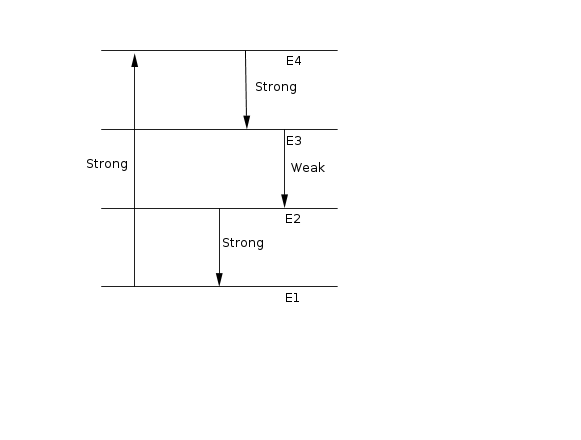
\includegraphics[width=0.75\textwidth]{figures/4state.png}
    \caption{Four state atom.}
    \label{fig:4state}
\end{figure}

While 3 state masers are possible, most actual masers involve 4 states. Lets discuss population inversion in a 4 state maser. We will relax the condition that collisions
be responsible for the transition to the highest state. As shown in the diagram we require that there is some strong transition from state 1 to 4. This provides atoms in a state that can dexcite to our population-inverted state. Imagine that we want states 3 and 2 to be the population inverted states. To achieve this, we need a relatively strong transition from state 4 to 3 to populate state 3. Similarly we need a strong 2 to 1 transition to empty out state 2. We are thus left with lots of atoms in state 3, and almost none in 2. This provides the inversion necessary for masing. Our masing transition will be 3 to 2 (ie it will correspond to our population inverted states).

\subsection{Class Notes}

MASERs, in some ways, are a throw-away topic. There is a whole lot of jargon that is too much for what we need -- but, they're cool and who doesn't like LASERs? 

What's the idea here? Let's go back to the basics. We have $\ato$ (spontaneous emission), $\bot$ (absorption), and $\bto$ (stimulated emission). Why did we cook these up? 

\be
\ato = \frac{2h\nu^3}{c^2}\bot
\ee

and 
\be
g_1 \bot = g_2 \bto
\ee

We got these by setting a rate equation:

\be
n_2 \ato = \left(n_1 \bot - n_2 \bto\right)J
\ee

We then asked this rate equation to reproduce the Planck function at LTE:

\be
B_\nu = \planck
\ee

In RTE:

\be
\frac{d I_\nu}{d s} = j_\nu - \alpha_\nu I_\nu
\ee

Here, we have:

\be
j_\nu = \frac{h\nu \ato n_2 \phi(\nu)}{4\pi}
\ee

\be
\alpha_\nu = \frac{1}{4\pi} h\nu \phi(\nu) \left(n_1 \bot - n_2 \bto\right)
\ee

So now let's go ahead and walk part way toward the Einstein relations. First, take the radiative transport equation, divide out $\alpha_\nu$:

\be
\frac{d I_\nu}{d\tau} = \underbrace{\frac{j_\nu}{\alpha_\nu}}_\text{source function} - I_\nu
\ee

We are left with:

\be
S_\nu = \frac{n_2 \ato }{n_1 \bot - n_2 \bto}
\ee

All of this is just a bunch of algebra, by the way. With a bit of algebra, we get:

\be
S_\nu = \frac{\frac{n_2 \ato}{n_2 \bto}}{\frac{n_1 \bot}{n_2 \bto} -1 }
\ee

The reason we got the Einstein relations at all was requiring that $S_\nu \to B_\nu = \planck$. In order for this to happen, we can see from the functional forms what must be equal. Note that we are not assuming LTE, bur rather just the Einstein coefficients. All of this amounts to:

\be
S_\nu = \frac{2h\nu^3}{c^2}\frac{1}{\frac{n_1 g_2}{n_2 g_1}-1}
\ee

This describes the radiation field for any excited-to-de-excited ratio. Let's play a thought experiment: what happens if $n_2/n_1 > g_2/g_1$? This is asking us to have more atoms in the excited state than if you had randomly assigned the energy. Let's do the algebraic implications first:

\be
\frac{n_1 g_2}{n_2 g_1} < 1 \rightarrow S_\nu < 0 
\ee

Does having a source function less than 0 even make sense? Well, negative power is not a real thing. You can have ``less'' power than another thing, but we cannot have negative power in a logical sense. But, we don't actually observe the source function. Instead, we observe specific intensity which is not the same thing as $S_\nu$. In a homogeneous medium, we know that the solution to the RTE:

\begin{equation}
    I_\nu (\tau) = I_{\nu,0} e^{-\tau} + \left(1-e^{-\tau}\right) S_\nu
\end{equation}

If we want to observe $S_\nu$, we have to observe it through some optical depth:

\be
\tau = \alpha_\nu s \text{ where } \alpha_\nu = \frac{1}{4\pi} h\nu \phi(\nu) \left(n_1 \bot - n_2 \bto\right)
\ee

We have the second term in $\alpha_\nu$ thus being negative, so both the source function and $\alpha_\nu$ being less than zero. Bad things have happened! Positing one thing, we now have a bunch of stuff being negative and crazy. But it all cancels out and gives real observables! 

Now the real question -- can $n_2/n_1 > g_2/g_1$ actually happen? If we look at Boltzmann statistics, this would tell us:

\be
\frac{n_2}{n_1} = \frac{g_2}{g_1} \underbrace{e^{-\frac{h\nu}{kT_{ex}}}}_{>1} \rightarrow T_{ex} < 0
\ee

Maybe instead of concluding that the temperature needs to be negative, we could say that we are ``not thermally stable.'' At best, we are in an unstable equilibrium. It would be energetically favorable to drop out of the equilibrium state. We would in fact call this ``non-thermal.'' This is a perfect time to introduce the three temperatures as measurements of distributions, and not some physical thing:

\begin{itemize}
    \item $T_\text{excitation}$ -- Measures distribution of atoms in a state. 
    
    \item $T_\text{kinetic}$ -- Measures distribution of velocities in a gas.
    
    \item $T_\text{brightness}$ -- Measures distributions of photon energies in a Planck function.
\end{itemize}

\textbf{When we say it's ``non-thermal,'' we say that we are not in a ``known'' distribution. It basically means that we have not settled into an equilibrium state.} 

We have some jargon for this -- a ``population inversion'' describes when $n_2/n_1 > g_2?/g_1$. But how do we make/impose a population inversion? Let's talk about a few different methods:

\begin{itemize}
    \item Collide atoms together. This is what we will talk about next class -- some of the kinetic energy goes into internal energy of the atoms. But as you start to have excited states, more collisions will de-excite. This is a great way to couple kinetic temperature $T_{kin}$ to excitation temperature $T_{ex}$. Eventually, we reach equilibrium between these two temperatures, so \textbf{we don't get a population inversion.}
    
    \item What about shinning some light on a system, driving the energy from lower states to upper states? This will cause stimulated emission, too, so we will recover Boltzmann statistics. This is a great way to couple the brightness temperature $T_{b}$ to the excitation temperature $T_{ex}$, so \textbf{we don't get a population inversion.}
    
    \item The truth? We will never get a population inversion by directly exciting the transition in question. If you are trying to get a population inversion directly, it is unavoidable to de-excited as well. We need to be a bit more circumspect about the population inversion. This leads to:
    
    \item Maybe we have more than one energy state, such as a three state atom. What if we now take the atoms in the $E_1$ state, and send them to $E_3$ with photons pumping energy. Maybe we could then get an excess in the $E_2$ state than you would have expected from the degeneracy. Thus, for the particular $E_2\rightarrow E_1$ transition, we have a population inversion. We also require the $E_1\rightarrow E_3$ transition to be strong and the $E_3\rightarrow E_2$ to be strong. However, critically, we need there to be a bit of a gap between $E_2\rightarrow E_1$ so that we can maintain the population inversion. This weak transition has a \textbf{much} longer timescale (smaller $\ato$). This will allow us to build up atoms in the state, and thus maintain a population inversion. It's even MORE effective if we have a 4-energy level system. It's also much more common to have a 4-state system. The diagram below is sort of an ideal case: 
    
    \begin{figure}
        \centering
        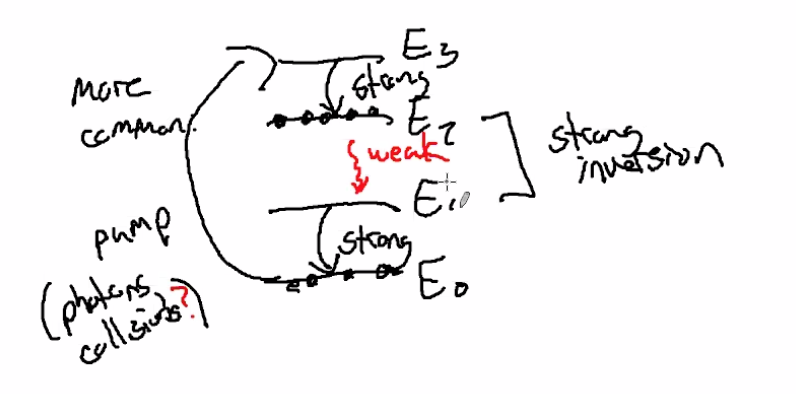
\includegraphics[width=0.75\textwidth]{figures/Screen Shot 2020-10-06 at 12.13.06 PM.png}
        \caption{MASER 4-energy states.}
        \label{fig:inv}
    \end{figure}
    
    \item In astronomy, the most common MASERs are $H_2 O$ and $OH$. We can see $OH$ MASERs across cosmological distances. 
\end{itemize}

So, what happens if you set something up like this? Remember where we came from:

\be
S_\nu = \frac{2h\nu^3}{c^2}\frac{1}{\frac{n_1 g_2}{n_2 g_1} - 1}< 0
\ee

We had both $\tau$ and $S_\nu$ $<0$. Returning to $\tau = \alpha_\nu s$, we can write:

\be
I_\nu (s) = \left(1 - e^{-\alpha_\nu s}\right) S_\nu
\ee

There is a regime in this equaiton where $I_\nu \propto e^{s}$. We call this an ``unsaturated'' MASER. What do we mean by this? Nothing has impeded the exponential growth. This cannot continue forever, so what clamps down on this growth? We reach a point where we don't have enough atoms to release MORE photons. The growth continues until we run out of atoms to be doubling our photons each time. When you run out of excited atoms, you can only pick up as many photons in the next unit of length as you have atoms in that same volume you crossed. There is thus a transition point to a saturated MASER, and in this regime, $I_\nu \propto s$. Of course, this depends all on the density of the excited atoms. A more dense environment will pick up more photons per length.

A steady state MASER will be limited by the pump. This gives a new way to think of MASERs. Where is the energy coming from? The excited state. So at some point, we are recovering the energy of the charge pump. Another way of interpreting the saturation point -- when the energy we are asking from the MASER is being outrun by the pump, we are saturated. 

Lastly, here are some random facts about MASERs:

\begin{itemize}
    \item It's easier to mase in low density environments. Atoms are colliding so infrequently that we can easily absorb the photons that give a population inversion. As long as we are provided a suitable energy pump/source such as stars.
    
    \item We also really need frequency coherence. This requirement turns into a velocity coherence argument since velocities turn into Doppler shifts. If we Doppler shift out of phase/frequency relative to the atoms we are going past (so that we are not at the resonated stimulated emission anymore), we cannot maintain a masing state. 
    
    \item In some ways, MASERs are similar to transistors. Often, turning on the transistor allows for amplified signals. The idea of a charge pump leading to amplified signal from a transistor is similar to the MASER. Here's a diagram of that analogy:
    
    \begin{figure}
        \centering
        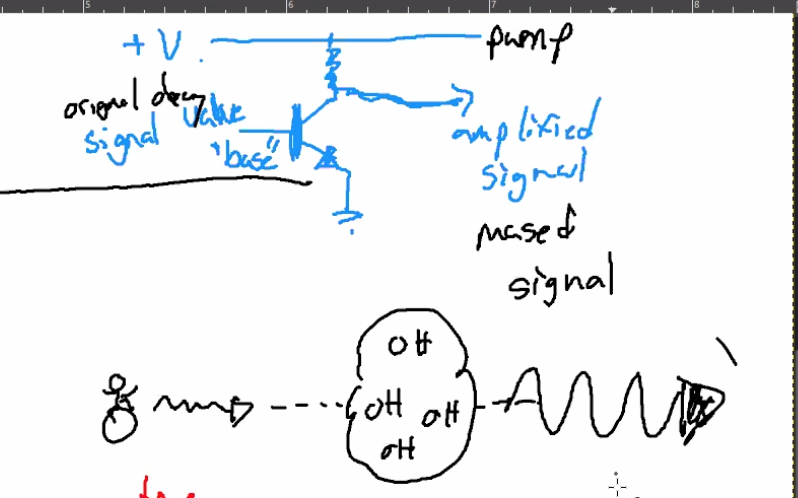
\includegraphics[width=0.75\textwidth]{figures/Screen Shot 2020-10-06 at 12.32.31 PM.png}
        \caption{OH MASER clouds and similarity to transistors. }
        \label{fig:transistor}
    \end{figure}
\end{itemize}




%%%%%%%%%%%%%%%%%%%%%%%%%%%%%%%%%%%%%%%%%%%%%%%%%%%%%%%%%%%%%%%%%%%%%%%%%%%%%%
%%%%%%%%%%%%%%%%%%%%%%%%%%%%%%%%%%%%%%%%%%%%%%%%%%%%%%%%%%%%%%%%%%%%%%%%%%%%%%
%%%%%%%%%%%%%%%%%%%%%%%%%%%%%%%%%%%%%%%%%%%%%%%%%%%%%%%%%%%%%%%%%%%%%%%%%%%%%%
\newpage
\section{October 8, 2020: Collisions}

\subsection{Detailed Balance}

Let's motivate the problem a bit. Consider an atom that undergoes a transition to an excited state. Let's consider state $E_0$ and $E_1$. The populations might all start in $E_0$, occasionally popping to $E_1$. If there was no reverse process, they would get stuck in $E_1$. Now suppose there is collisional de-excitation, where say a collisions takes the energy and converts it to kinetic energy of the incoming particle. 

Let's call $P_{01}$ the probability to transition to the excited state, and $P_{10}$ being the reverse process. Now consider what happens in the same scenario! Preferrentially, at the beginning, atoms will get excited. Once we have some population is excited, they will start to reverse back to the ground state. This eventually reaches equilibrium -- the rate going to the excited state is equal to the rate coming back down:

In thermal equilibrium:

$$
r_{01} = n_0 P{01} \overbrace{c}^\text{collision rate} = r_{10} =  n_1 P{10} \overbrace{c}^\text{collision rate}
$$

We don't necessarily have to have the probabilities being equal. Instead, we can have pileups as implied by the dependence on the number density. This system is easy to solve for. 

Three state systems are much more complicated since there are many more transition processes. You can imagine in this case that:

$$
r_{01} = \left(n_0 P_{01} + n_0 P_{02} P_{21}\right)c
$$

This doesn't account for even more esoteric ways of transitioning -- this is only three states, too! Therefore, the complexity RAPIDLY increases with the number of states. 

This is where the idea of \textbf{detailed balance} comes in. For some systems (see caveats), you don't need to worry about ALL the pathways between energy states. Instead, in thermal equilibrium, \textbf{each basic process will be balanced by its exact reverse.} This means that we just balance each fundamental process by its own inverse and none of the other pathways. This simplifies life \textbf{dramatically.} We can therefore do things like:

$$
n_0 P_{01} c = n_1 P_{10} c 
$$

Simply on the ratios of probabilities will give us the relative populations. What are the caveats?


Here is a figure that summarizes the above text: 
\begin{figure}
    \centering
    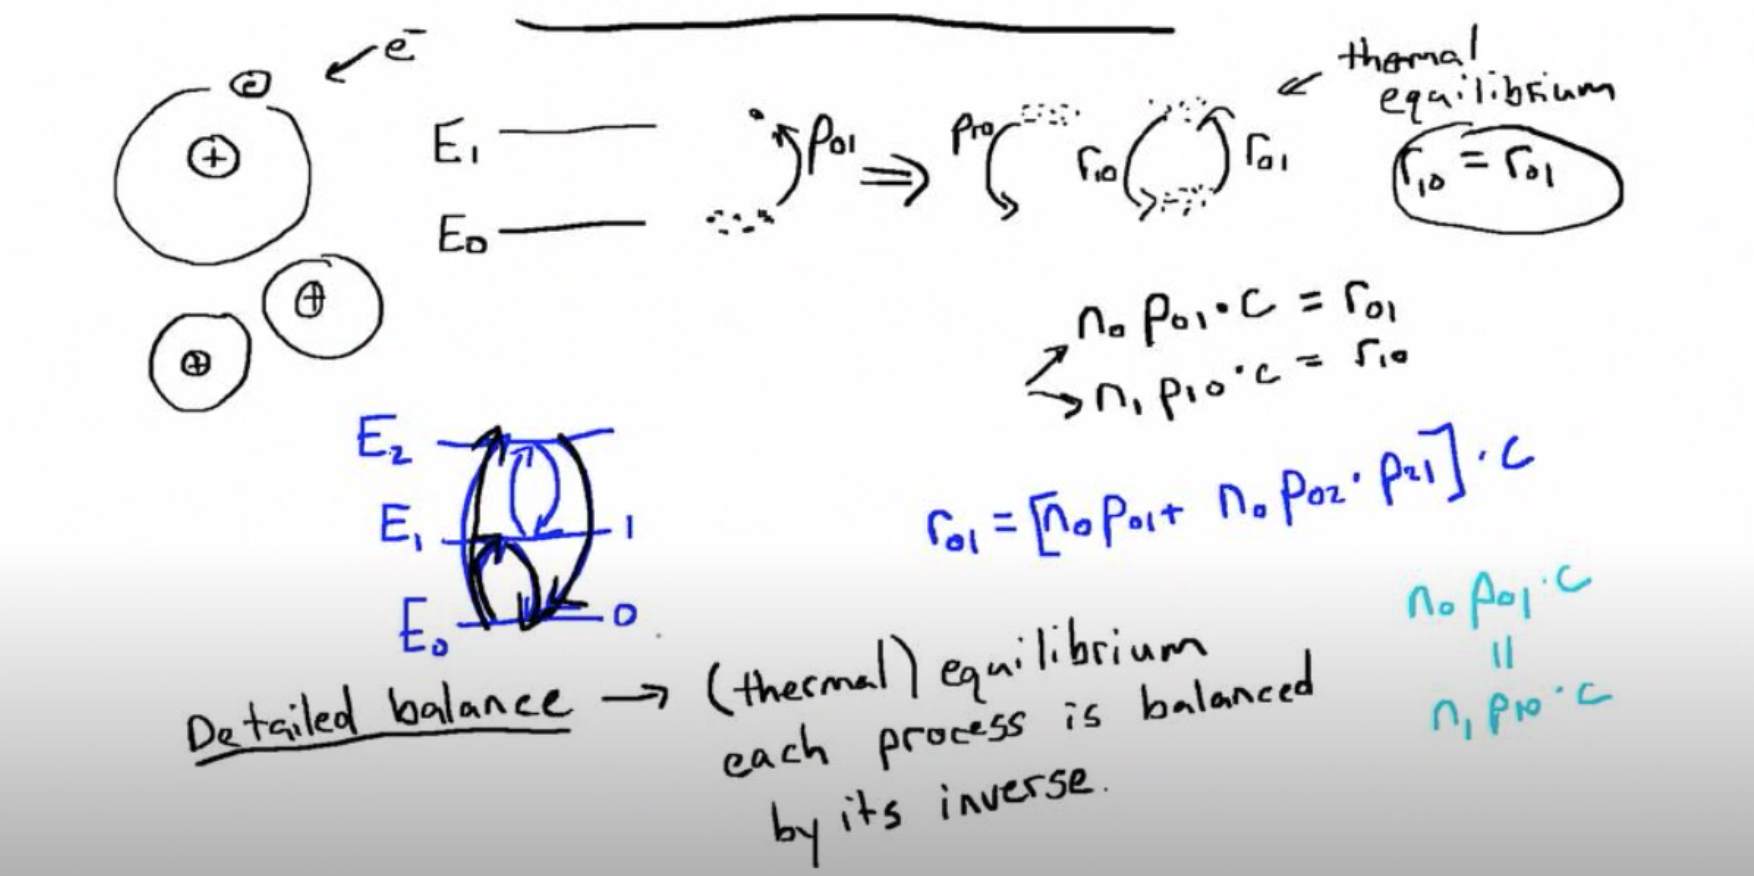
\includegraphics[width=0.75\textwidth]{figures/Screen Shot 2020-10-10 at 7.22.32 PM.png}
    \caption{Summary of the above text, from top left to bottom right. }
    \label{fig:summmmm}
\end{figure}


The caveats? Let's consider a system where it doesn't work. Consider three states $0,1,$ and $2$. We can go in all directions between states. Let's assign some strange probabilities, too:

\begin{figure}
    \centering
    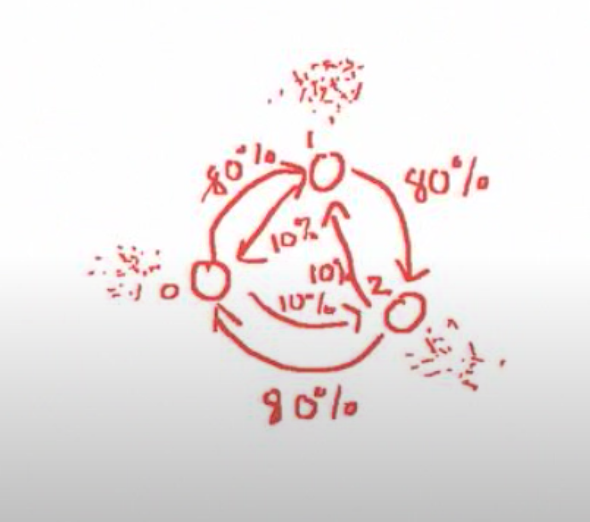
\includegraphics{figures/Screen Shot 2020-10-10 at 7.25.44 PM.png}
    \caption{Consider starting some population in state 1. You can see from the symmetry of the problem, equal numbers of atoms will pile up on the outer edge, and the small reverse process probabilities prevent detailed balance from being achieved. So what went wrong? }
    \label{fig:detbalancefailure}
\end{figure}

\textbf{The Kolmogorov Criterion:} Detailed balance only works if probabilities around closed loops match forward and backward. Otherwise, other pathways dominate the flow of atoms. However, lots of systems do follow the Kolmogorov Criterion. But, occasionally, you don't, so it's nice to know about it!


\subsection{Detailed Balance (Aaron's Notes)}

The Einstein analog:
$$\overbrace{A}^{low\ E\ particle} + \overbrace{B_{fast}}^{high\ E\ e^-}
\to \overbrace{A^*}^{excited} + B_{slow}$$
So the Rate of Excitations $R_{ex}$ is given by:

\def\rex{R_{ex}}
\def\vrel{v_{rel}}
$$\rex = n_An_B\sigma_{12}f(\vrel)\vrel$$
Suppose we have some distribution of relative velocities given by $f(v)dv$,
where $f$ is the fraction of collisions occurring with relative velocities
$[\vrel, \vrel +dv]$.  Then:
$$\rex = n_An_B\int_0^{\infty}f(v)dv\sigot(v)v$$
$$=n_An_B \mean{\sigot v}$$
\def\qot{q_{12}}
\def\qto{q_{21}}
$$=n_An_B\qot$$
where $\qot$ is the ``collisional rate coefficient'' $[cm^3s^{-1}]$.  Then the
Rate of de-excitation is given by:
$$R_{deex} = n_An_B\int_0^\infty{f(v)v\,dv\sigma_{21}(v) = n_A^*n_B\qto}$$
We recognize now that $\sigot(v)n_An_Bf(v)dv\,v$ is the rate of excitations of 
A using B moving at relative velocity $v$.  If we have detailed balance,
then this has to be the same as the rate of de-excitation
$n_A^*n_Bf(v^\prime)v^\prime\sigto(v^\prime)$.
$$\overbrace{\frac12 m_rv^2}^{center\ of\ mass\ E} = hv_{12} + \frac12 m_rv^{\prime2}$$
Where $m_r$ is the reduced mass $\frac{m_A m_B}{m_A+m_B}$. However many $B_{slow}$
are created by collisional excitation, the same number are used for the
reverse de-excitation.  This is {\bf detailed balance}.\par


\subsection{Collisional Excitations}

The basic picture -- we have an atom with an electron, and another particle that flies in. The atom moving is particle B. This puts the atom in an excited state, with particle B having a different velocity $v'$, leaving a population in the excited state $n_A^*$. Consider conservation of energy:

$$
\frac12 \mu v^2 \rightarrow h \nu_{12} + \frac12 \mu v'^{2}
$$

Now we want to know the rates of excitation for these atoms for a distribution of B particles coming in. Consider some A particles in a box with some B particles moving around. What is the collision rate per unit volume? We have said before that:

$$
\lambda_{mfp}^{-1} = n_a \sigma_{12} 
$$

We can turn this into a collision rate:

$$
C_{12} = n_A \sigma_{12} v_{rel} = n_a \sigma_{12} \frac{v}{\lambda_{mfp}}
$$

If we want to talk about this per unit volume, we need $n_B$ as well:

$$
n_B C_{12} = n_B n_A \sigma_{12} v_{rel}
$$

We have a problem here -- we only have one velocity! What if we have a distribution of velocities? In that case, we want the number density $n_B$ as a function of velocity times some differential interval in velocity. 

$$
n_B C_{12} = n_B n_A \overbrace{\underbrace{\int_{0}^{\infty} f(v) \sigma_{12}(\nu) v_{rel} dv}_\text{weighted average, really}}^{\langle \sigma_{12} v\rangle \equiv q_{12}}
$$

We call $q_{12}$ the collisional rate coefficient, and has units of $\cm^3 \s^{-1}$. We thus have an expression for the rate of transitions from energy state 1 to 2 per unit volume:

$$
n_B C_{12} = n_A n_B q_{12}
$$

Consider what this looks like for a two-state atom in the most general sense:

$$
\boxed{\overbrace{n_A \left[\underbrace{B_{12} \bar{J}}_\text{absorption} + \underbrace{n_B q_{12}}_\text{collisional excitation} \right]}^\text{ways to excite an atom} = \overbrace{n_A^* \left[\underbrace{A_{21}}_\text{spont. decay} +  \underbrace{B_{21}\bar{J}}_\text{stimulated emission} + \underbrace{n_B q_{21}}_\text{collisional de-excitation} \right]}^\text{ways to de-excite an atom}}
$$

where

$$
q_{12} \equiv \int_{0}^{\infty} f(v) \sigma_{12} v dv.
$$

Let's take a limit of this where we have a weak radiation field and our time-constants for spontaneous emission are long compared to collision rates. This allows us to neglect the radiative terms with $\bar{J}$ and $A_{21}$ and assume we are in a collisionally dominated system. Adding in the fact that we are in equilibrium, this gives:

$$
n_A n_B q_{12} = n_A^* n_B q_{21}
$$

We thus see we are independent of $n_B$. We only care about the colliding particles in the sense that they give us collisionally dominated systems. Other than that, we have no dependence on B particles! 

We still have a bit of a complication. The two $q$ collisional rate coefficients are integrals over all velocities. However, we are using two different velocities on both sides of the equation above. So, in general, the integrals for $q_{12}$ and $q_{21}$ have different velocities. We can use detailed balance to rescue us! We can therefore drop the velocity integrals and consider only two velocities:

$$
n_A f(v) \sigma_{12} v = n_A^* f(v') \sigma_{12} v'
$$

However this only holds over a range $dv$ in velocity space on each side. Let's impose a few more constraints (since we have only assumed statistical equilibrium so far). Let's not plug in the Maxwellian distribution for these:

$$
f(v) = \left(\frac{m r}{2\pi kT}\right)^{3/2} 4 \pi v^2 e^{-\frac{\frac12 m v^2}{kT}} 
$$

We thus have:

$$
n_A v^2 e^{-\frac{\frac12 m v^2}{kT}} \sigma_{12} v = n_A^* v'^2 e^{-\frac{\frac12 m v'^2}{kT}} \sigma_{21} v' 
$$

The assumption of Maxwellian distribution for velocity also implies thermal equilibrium -- giving us Boltzmann statistics for the population statistics:

$$
\frac{n_A^*}{n_A} = \frac{g_A^*}{g_A} e^{-\frac{h\nu}{kT}}
$$

Plugging in for $n_A^*$, we get:

$$
v^3 e^{-\frac{\frac12 m v^2}{kT}} \sigma_{12}  dv = \frac{g_A^*}{g_A} e^{-\frac{h\nu_{21}}{kT}} v'^3 e^{-\frac{\frac12 m v'^2}{kT}} \sigma_{21} v' dv'
$$

When we multiply the two exponentials, cool things happen! The exponentials all cancel since the argument becomes the total energies! We can do one last cool thing. Because we have energy conservation, we can take the derivatives of energy conservation with respect to $v$ to show that $v dv = v' dv'$, giving: 

$$
g_1 v^2 \sigma_{12}(v) = g_2 v'^2 \sigma_{21}(v') 
$$


\section{Collisional Excitations (Aaron's Notes)}

The analog of Einstein Coefficients:
$$\overbrace{A}^{low\ E\ particle} + \overbrace{B_{fast}}^{high\ E\ e^-}
\to \overbrace{A^*}^{excited} + B_{slow}$$
So the Rate of Excitations $R_{ex}$ is given by:

\def\rex{R_{ex}}
\def\vrel{v_{rel}}
$$\rex = n_An_B\sigma_{12}f(\vrel)\vrel$$
Suppose we have some distribution of relative velocities given by $f(v)dv$,
where $f$ is the fraction of collisions occurring with relative velocities
$[\vrel, \vrel +dv]$.  Then:
$$\rex = n_An_B\int_0^{\infty}f(v)dv\sigot(v)v$$
$$=n_An_B \mean{\sigot v}$$
\def\qot{q_{12}}
\def\qto{q_{21}}
$$=n_An_B\qot$$
where $\qot$ is the ``collisional rate coefficient'' $[cm^3s^{-1}]$.  Then the
Rate of de-excitation is given by:
$$R_{deex} = n_An_B\int_0^\infty{f(v)v\,dv\sigma_{21}(v) = n_A^*n_B\qto}$$
We recognize now that $\sigot(v)n_An_Bf(v)dv\,v$ is the rate of excitations of 
A using B moving at relative velocity $v$.  If we have Detailed Balance,
then this has to be the same as the rate of de-excitation
$n_A^*n_Bf(v^\prime)v^\prime\sigto(v^\prime)$.
$$\overbrace{\frac12 m_rv^2}^{center\ of\ mass\ E} = hv_{12} + \frac12 m_rv^{\prime2}$$
Where $m_r$ is the reduced mass $\frac{m_Am_B}{m_A+m_B}$. However many $B_{slow}$
are created by collisional excitation, the same number are used for the
reverse de-excitation.  This is {\bf Detailed Balance}.\par
Second, under thermal equilibrium, particles have a {\bf Maxwellian velocity distribution}:
$$\boxed{f(v)=4\pi\left(\frac{m_r}{ 2\pi kT}\right)^\frac{3}{ 2}v^2
e^\frac{-m_rv^2}{2kT}}$$
\centerline{(Maxwellian velocity distribution)}
In thermal equilibrium (see Boltzmann distribution),
$$\frac{n_A^*}{ n_A} = \frac{g_2}{ g_1}e^\frac{-h\nu_{21}}{ kT}$$
Now, assuming detailed balance and thermal equilibrium,
$$n_An_Bf(v)dv\,v\sigot=n_A^*n_Bf(v^\prime)dv^\prime v^\prime \sigto$$
\def\emvkt{e^\frac{-m_rv^2}{2kT}}
\def\emvpkt{e^\frac{-m_rv^{\prime2}}{2kT}}
\def\ehvkt{e^\frac{-h\nu_{21}}{2kT}}
$$\sigot v^2\emvkt = \frac{g_2}{t_1}\ehvkt \nu^{\prime2}\emvpkt v^\prime 
dv^\prime\sigto$$
$$\sigot dv\,v^3 \emvkt = \frac{g_2}{t_1}\ehvkt \ehvkt \emvkt v^{\prime3}
dv^\prime \sigto$$
$$\boxed{g_1v^2\sigot(v) = g_2v^{\prime2}\sigto(v^\prime)}$$
This is the analog of the relationship between the Einstein coefficients $B_{12}$ and $B_{21}$.

For a specific case, $B=e^-$, $A=$ion with bound electron.

\subsection{ More on Einstein Analog }
Forgot something for the Einstein Coefficients Analog.  Recall:
$$g_1v^2\sigma_{12}(v)=g_2v^{\prime2}\sigma_{21}(v^\prime)$$
$$\hf m_rv^2=h\nu_{21}+\hf m_r(v^\prime)^2$$
For the special case of $f(v)$ being a Maxwellian velocity distribution, then:
$$\frac{q_{12}}{q_{21}}\equiv\frac{\mean{\sigma_{12}v}}{\mean{\sigma_{21}v}}
=\frac{g_2}{g_1}e^\frac{-h\nu_{21}}{kT}$$
This has a Boltzmann factor, which makes you thing we're assuming LTE, but
we're not. \par
Last time, we were talking about electron-ion collisional excitation, given by:
$$\qot\equiv\mean{\sigot v}\propto\inv{v}\propto T^{-\hf}$$
We can extend this for neutral-ion collisional excitation:
$$\qot \propto T^\hf T^{-\hf} \propto T^0$$
$$\sigot\equiv\frac{\pi\hbar^2}{ m_ev^2}\frac{\Omega(1,2)}{ g}$$
where $\Omega(1,2)$ scales as $T^\hf$.  Notice this means that for some
neutral-ion collisional excitation, it is {\it temperature independent}.
For neutral-neutral collisional excitation:
$$\qot=\mean{\sigot v}\propto T^\hf$$
$$\sigot\propto T^0\sim \pi(Fa_0)^2$$
This is all we'll talk about bound-bound transitions.


\subsection{Class Notes}

\begin{figure}
    \centering
    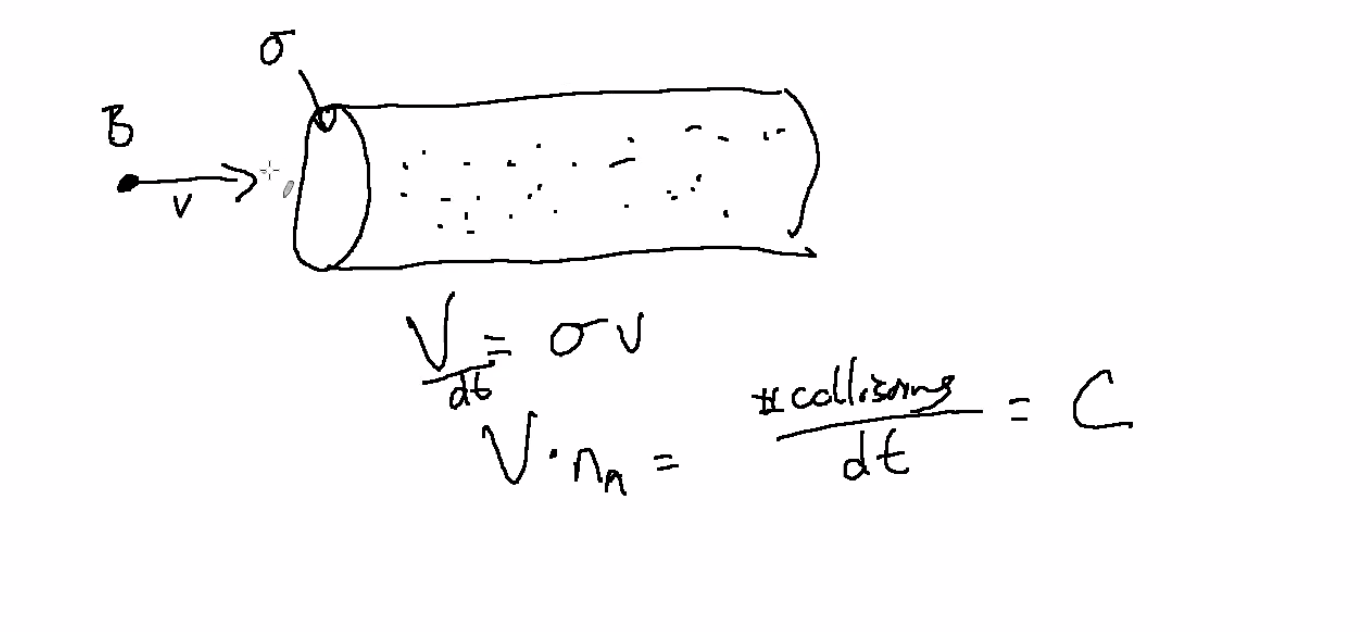
\includegraphics[width=0.75\textwidth]{figures/Screen Shot 2020-10-08 at 11.20.59 AM.png}
    \caption{Here is a picture to explain the collision coefficients. We also picked a $B$ particle, and we ask how many $A$ particles does it hit. If we want to track an $A$ particle, we need to pick an $A$ particle, track its velocity with respect to the $B$ particles. We need to always keep track of the particles we are colliding.}
    \label{fig:coeffs}
\end{figure}

One thing that was not mentioned in the video -- electrons are often the ones that are colliding since they are so light. However, very cold and neutral things like molecular clouds becomes molecular collisions. Often, our cross section FOR PHYSICAL COLLISIONS (not photon absorption, for example) is approximately:

\be
    \sigma \sim \pi a_0^2
\ee

%%%%%%%%%%%%%%%%%%%%%%%%%%%%%%%%%%%%%%%%%%%%%%%%%%%%%%%%%%%%%%%%%%%%%%%%%%%%%%
%%%%%%%%%%%%%%%%%%%%%%%%%%%%%%%%%%%%%%%%%%%%%%%%%%%%%%%%%%%%%%%%%%%%%%%%%%%%%%
%%%%%%%%%%%%%%%%%%%%%%%%%%%%%%%%%%%%%%%%%%%%%%%%%%%%%%%%%%%%%%%%%%%%%%%%%%%%%%
\newpage
\section{October 13, 2020: Free-Free Emission}

\subsection{Thermal Bremsstrahlung}

Braking radiation is the German-to-English translation! Consider a free streaming electron of charge $-e$ passing by an ion with charge $Z$. The interaction will cause emission of radiation from the acceleration. It radiates according to Larmor Power:

$$
P = \frac23\frac{e^2 a^2}{c^3}
$$

Consider an electron passing a distance $B$ from the nucleus. The acceration is given by:

$$
\ddot{x} \sim \frac{Ze^2}{b^2 m_e}
$$

Plugging this in above:

$$
P \sim \frac{2}{3} \frac{Z^2 e^6}{b^4 m_e^2 c^3}
$$

We can estimate the energy as the power times a time. But where does the time come from? It's approximately the time it takes for the interaction to start and then end. This is approximately the electron crossing a distance $2b$ at a velocity $v$:


$$
E \sim \frac{4}{3}\frac{Z^2 e^6}{b^4 m_e^2 c^3} \frac{b}{v}
$$

We will now do something a bit wonky! We will relate the distance $b$ to a frequency -- in a hand-wavy sense, the acceleration of the electron looks like a sine wave. When it is approaching, the electron is being pulled in. There is an instant at which the electron is in circular accleration, and then afterwards, the electron is getting pulled backward by the electric force. Graphing this over time is approximately sinusoidal:

$$
\frac12 T \sim \frac{2b}{v} \rightarrow \nu \sim \frac{v}{4b} \rightarrow d\nu \sim \frac{-v}{4b^2} db
$$

This, plain and simply, relates the frequency of radiation to the closeness of the electron and ion. 

\begin{figure}
    \centering
    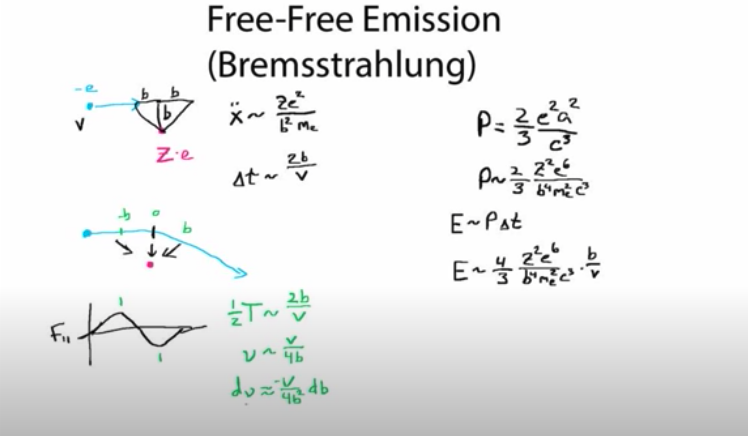
\includegraphics[width=0.74\textwidth]{figures/Screen Shot 2020-10-11 at 11.54.09 PM.png}
    \caption{Summary of the above text.}
    \label{fig:summmm2m2m}
\end{figure}

Now consider a bunch of electrons passing around a nucleus. How many of those electrons are passing by at a distance $b$ from the nucleus? Those are the ones radiating, anyways. There is a derivation here, hand-wavy, for this differential power:

$$
dP \sim E 2\pi b db n_e v
$$

If we plug in for $E$ and $db$:

$$
\frac{dP }{d\nu} \sim \frac{-32\pi}{e} \frac{Z^2 e^6 n_e}{m_e^2 c^3 v}
$$

There is no factor of $b$! We can also consider the velocity to be Maxwellian, but we need to be a bit careful. If an electron is moving too slowly, the electron will be captured. Thus, there is a minimum velocity -- a velocity such that the kinetic energy is of order the photon given off by acceleration:

$$
\boxed{\langle\frac{dP}{d\nu}\rangle = \int_{\nu_{min}}^{\infty} \frac{dP}{d\nu} f(v) dv = \frac{64 \sqrt{\pi}}{3\sqrt{2}} \frac{Z^2 e^6 n_e}{m^{3/2} c^3 \sqrt{kT}} e^{-\frac{h\nu}{kT}}}
$$

If we want to calculate our emissivity $j_{\nu,ff}$:

$$
\boxed{j_{\nu,ff} = \frac{16}{3\sqrt{2\pi}} \frac{Z^2 e^6 n_e n_p}{m^{3/2} c^3 \sqrt{kT}} e^{-\frac{h\nu}{kT}}}
$$

If we want to be SUPER explicitly exact, we have to add what's called the ``Gaunt factor'' -- a quantum mechanical correction that is of order unity:

$$
\boxed{j_{\nu,ff} = \frac{16}{3\sqrt{2\pi}} \frac{Z^2 e^6 n_e n_p}{m^{3/2} c^3 \sqrt{kT}} e^{-\frac{h\nu}{kT}} \underbrace{\frac{\pi}{\sqrt3} \bar{g}_{ff}(v,T)}_\text{Gaunt factor}}
$$

For every forward process, there is a reverse process! We can have an electron absorb a proton and GAIN energy in the process. Let's definine $\alpha_{\nu,ff} \equiv \frac{j_{\nu,ff}}{B_{\nu}}$. This is just to say that in the optically thick limit, the $I_\nu \to S_\nu = j_\nu / \alpha_\nu$. This reverse process is calle \textbf{inverse bremsstrahlung}. Sometimes we want to write this as an opacity:

$$
\kappa_{\nu,ff} = \frac{\alpha_\nu}{\rho} \propto \frac{n_e n_p}{\rho}T^{-3.5}
$$

This is what we call \textbf{Kramer's Opacity}, which is used for stellar evolution very frequently. 

$$
\boxed{\kappa_{\nu,ff} \propto \rho T^{-3.5}}
$$

Perhaps more usefully, we can include the coefficient of proportionality: 

$$
\boxed{\kappa_{\nu,ff} = \frac{\rho} {\left(3 \times 10^{23}\right)T^{3.5}} \cm^{2} \g^{-1}}
$$

The key takeaway is that Kramer's Opacity comes from inverse bremsstrahlung.

\textbf{Let's return to our assumptions:}

\begin{itemize}
    \item We assumed a Maxwellian distribution for velocity for electrons, which is okay because the collision time scale is smale, relaxing into an MB quickly.
    \item This is also non-relativistic, so we are making maximum temperature assumptions. This temperature is roughly $10^{10} \K$. Otherwise, we need relativisitic bremsstrahlung. 
\end{itemize}


\subsection{Thermal Bremsstrahlung (Aaron's Notes)}

\subsubsection{ Bremsstrahlung (braking radiation)}

Bremsstrahlung is the continuum of emission from a plasma caused by
the deflection of charged particles off of one another.  It is a common source of X-ray emission.
The deflection we will discuss, which is the most important, is of an $e^-$ by a positive nucleus, where we assume the nucleus to be stationary.


\begin{figure}
    \centering
    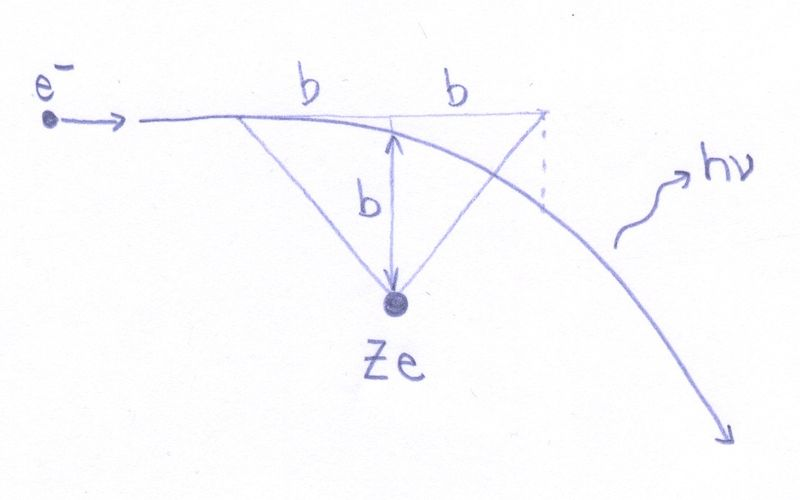
\includegraphics[width=0.75\textwidth]{figures/800px-Bremsstrahlung.jpg}
    \caption{Thermal Bremsstrahlung}
    \label{fig:thermBremsstrahlung}
\end{figure}


Recall that the power radiated by an accelerated
$e^-$ is (see Larmor Formula):
$$P=\frac{2}{3}\frac{e^2a^2}{ c^3}$$
In this case, the acceleration is due to the electric force of a
nucleus, so $a\sim\frac{Ze^2}{ b^2m_e}$, where $b$ is the distance of
closest approach between the $e^-$ and the nucleus, known as the impact parameter.  Thus:
$$P=\frac{2}{3}\frac{Z^2e^6}{ b^4m_e^2c^3}$$
The energy released by this encounter is given by $E \,\sim\, P\Delta t$, where
$\Delta t$ is the time of interaction.  We can approximate the interaction to occur roughly over a distance $b$ to either side of the nucleus, and so, if the $e^-$ is traveling at a speed $v$, then
$\Delta t\sim\frac{2b}{ v}$.  Therefore:
$$E\sim\frac{4}{3}\frac{Z^2e^6}{ m_e^2c^3b^4}\frac{b}{ v}$$
From the $e^-$ 's point of view, the force of the nucleus's $\ef$ is initially pulling the $e^-$ almost directly forward, and ends up pulling
the $e^-$ nearly completely backwards.  At the point of closest approach, the $e^-$ is not being pulled forwards or backwards, the electric force is solely perpendicular to the original direction of motion. We can therefore see that if we plot the parallel component of the force, we end up with something that looks a lot like a sine wave of period $2\Delta t$.  
\begin{figure}
    \centering
    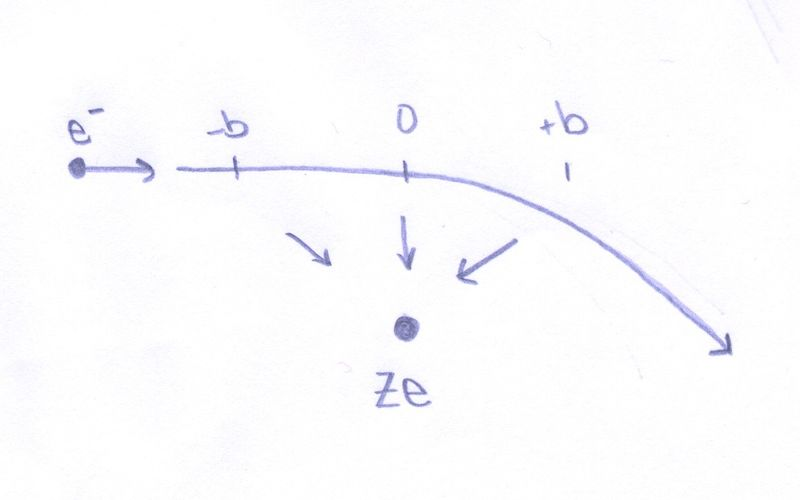
\includegraphics[width=0.75\textwidth]{figures/800px-InteractionRange.jpg}
    \caption{Region in which the electron and nucleus are ``interacting.''}
    \label{fig:intRange}
\end{figure}
\begin{figure}
    \centering
    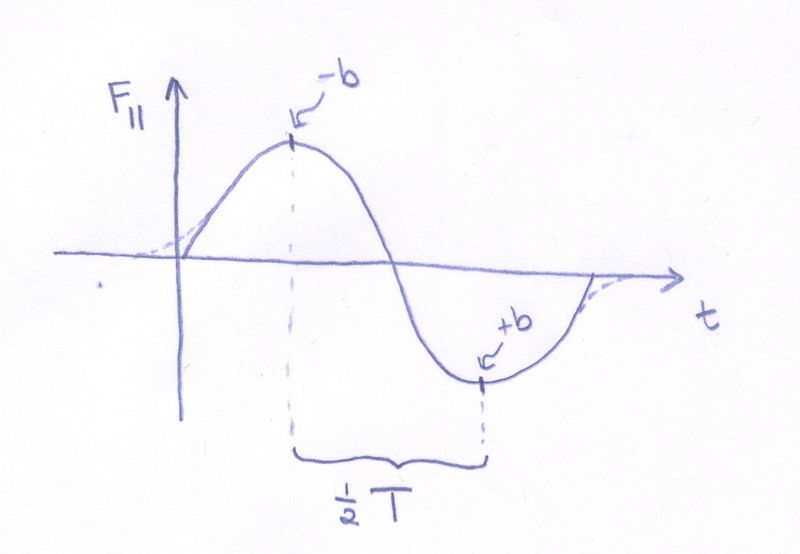
\includegraphics[width=0.75\textwidth]{figures/800px-ParallelForce.jpg}
    \caption{Parallel component of the Electric Force from the electron’s point of view.}
    \label{fig:parforce}
\end{figure}
From earlier, we know though that $\Delta t\sim\frac{2b }{ v}$.  Multiplying this by 2 in order to get a period, and inverting it to get a frequency, we have $\nu\sim\frac{v }{ 4b}$.  
This enables us to relate $d\nu$ to
$db$, which will be useful to us in a minute:
$$d\nu\sim{-\frac{v}{4b^2}}db$$
Now let's consider a nucleus in a sea of electrons.  
\begin{figure}
    \centering
    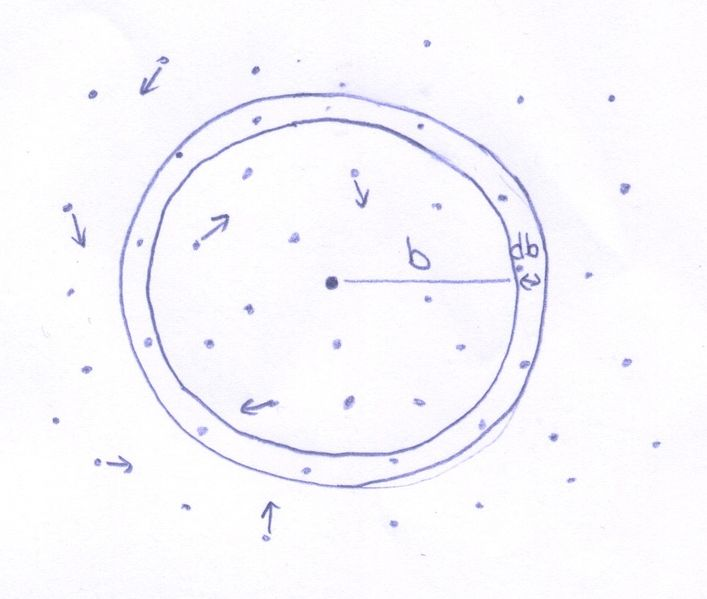
\includegraphics[width=0.75\textwidth]{figures/707px-ElectronSea.jpg}
    \caption{Sea of Electrons}
    \label{fig:sea}
\end{figure}
The electrons of interest to us are those a distance $b$ from the nucleus.  This fraction of electrons is given by the number density of electrons multiplied by the area of the ring: $2\pi b\,db\,n_e$.
Thus, the power radiated by that ring is:
$$dP\sim E\cdot 2\pi b\,db\,n_ev$$
where we need to include the $e^-$ velocity to account for the increased interaction rate for fast moving electrons. 
Using our relation between $d\nu$ and $db$, and our expression for $E$ we arrive at:
$$\frac{dP}{ d\nu}\sim\frac{-32\pi}{3}\frac{Z^2e^6n_e}{ m_e^2c^3v}$$
So the power per frequency interval is independent of distance!\par
The remaining term left to define is the velocity.  We have seen that in a plasma, the collision rates between electrons are high enough to relax into a Maxwellian velocity distribution fairly quickly:
$$f(v)=\left(\frac{m_e}{2\pi kT}\right)^\frac{3}{2}4\pi v^2 e^{-\frac{m_ev^2}{2kT}}$$
However, we are considering free-free emission, and so we must define a minimum velocity below which the electron would otherwise get captured by the nucleus. An $e^-$ with this minimum velocity will have a kinetic energy of order the energy radiated by the acceleration, which is the energy of a photon: $h\nu\sim\hf mv_{min}^2$.  Then
the average total power released over all velocities due to the interaction with one nucleus is:
$$\begin{aligned}\mean{\frac{dP}{ d\nu}}&=\int_{v_{min}}^\infty{\frac{dP}{ d\nu}4\pi
\left(\frac{m_e}{2\pi kT}\right)^\frac{3}{2}e^{-\frac{m_ev^2}{2kT}}v^2dv}\\ 
&=\frac{64\sqrt{\pi}}{3\sqrt{2}}\frac{Z^2e^6n_e}{ m_e^\frac{3}{2}c^3(kT)^\hf}
e^{-\frac{h\nu}{ kT}}\\ \end{aligned}$$
where the $h\nu$ in the exponential is from the lower velocity bound which we just defined.
\def\jnff{j_{\nu,ff}}
We now define $\jnff$ to be the volume emissivity for free-free interactions.
That is, $\jnff$ measures the power radiated by plasma, per volume, into
a solid angle $d\Omega$.  We can calculate the ``per $d\Omega$'' because the
radiation is isotropic:
$$\boxed{\jnff=\frac{16}{3\sqrt{2\pi}}\frac{Z^2e^6}{ m_e^\frac{3}{2}c^3(kT)^\hf}
n_en_pe^{-\frac{h\nu}{ kT}}}$$
where we have to include the \# density of ions, $n_p$, as well to account for the contribution from multiple nuclei.  This is the expression for
Thermal Bremsstrahlung.  Note that the definition of $\jnff$ in Rybicki \&
Lightman has an additional factor of $\frac{\pi}{\sqrt{3}}\,\bar{g}_{ff}(v,T)$, which
is a quantum mechanical correction factor of order unity.  It's called the
``Gaunt factor''.

\subsubsection{ Inverse Bremsstrahlung}

We now consider the inverse effect, an $e^-$ can also absorb a photon and become more energetic and ``free''.  
\begin{figure}
    \centering
    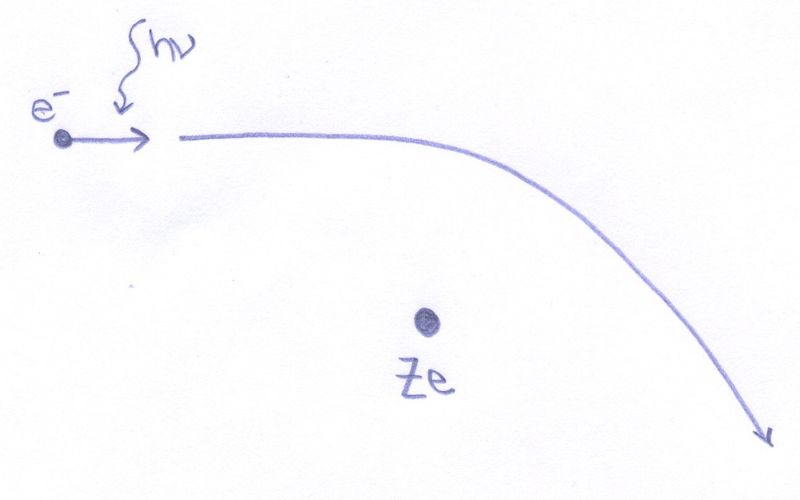
\includegraphics[width=0.75\textwidth]{figures/800px-InvBremsstrahlung.jpg}
    \caption{Inverse Bremsstrahlung}
    \label{fig:inBremsstrahlung}
\end{figure}
We define the coefficient for thermal free-free absorption as:
\def\anff{\alpha_{\nu,ff}}
$$\anff\equiv\frac{\jnff}{ B_{\nu}}$$
where we use the Planck function because we know that in the optically thick case the specific intensity, $I_{\nu}$, becomes the source function, $S_{\nu}=\frac{\jnff}{ \anff}$, and in the case of optically thick thermal radiation, the source function becomes the Planck function. And so, just as the expression for $\jnff$ was the definition of Thermal Bremsstrahlung, the expression for $\anff$ is the definition for Inverse Bremsstrahlung. 
$$\boxed{\anff=\frac{8}{3\sqrt{2\pi}}\frac{Z^2e^6}{ m_e^\frac{3}{2}c(kT)^\hf}\frac{n_en_p}{ h\nu^3}\left({1-e^{-\frac{h\nu}{ kT}}}\right)}$$
where we can once again include a factor of $\frac{\pi}{\sqrt{3}}\,\bar{g}_{ff}(v,T)$ to obtain the same result as Rybicki \&
Lightman. In the regime where $h\nu\gg kT$ the exponential term becomes negligible and the absorptivity will go as $\,\nu^{-3}$. The $h\nu\ll kT$ regime is the Rayleigh-Jeans regime and the expression for absorptivity goes as $\,\nu^{-2}$, where we have lost a factor of ${\,1/\nu}$ due to the Taylor expansion of the exponential.

\subsection{Opacity (Aaron's Notes)}

\subsubsection{Opacity}

Opacity measures how effectively a microscopic process of absorption or scattering reduces radiation traveling along a line of sight. Absorption is the destruction of photons when they converted into other forms of energy. Scattering is the absorption of photons coming from one direction that are then re-emitted into other directions, reducing the amount of radiation along a given line of sight. Scattering can either by a continuum process, such as Compton Scattering, or a line process, such as photo-excitation of electrons from a ground state to an excited state that then fall back into that same ground state.

\begin{figure}
    \centering
    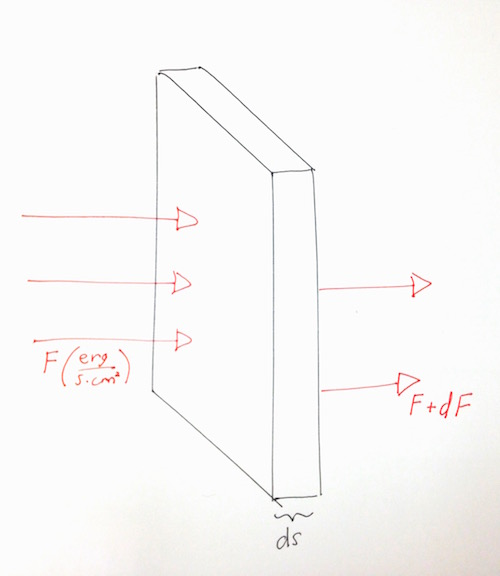
\includegraphics[width=0.75\textwidth]{figures/Flux1.jpg}
    \caption{Flux}
    \label{fig:flux}
\end{figure}

We consider the radiative flux incident on a slab of gas of a given density and how the opacity reduces the outgoing flux along the line of sight. The amount of flux exiting the slab depends on the width of the slab, the density, and the effectiveness of the absorption/scattering which we will call the opacity. Each of these factors reduces the amount of radiation that can flow through the slab and therefore the flux is reduced. 

$$
\begin{aligned}
dF &= -\kappa \rho F ds \\
\frac{dF}{ds} &= - \kappa \rho F
\end{aligned}
$$

Many absorption and emission processes are frequency dependent and anisotropic, and therefore we transform this flux into a specific intensity. We also can equate the product of opacity and density to the absorption coefficient to obtain a similar form as the Radiative Transfer Equation where there is assumed to be no emission.

$$
\begin{aligned}
\frac{dI}{ds} &= - \alpha_\nu I \\
\alpha_\nu &=  \kappa_\nu \rho
\end{aligned}
$$

In general, opacity has a power law dependence on both the density of the gas as well as its temperature.

$$ \kappa \simeq \rho^a T^b $$

The opacity is a macroscopic parallel to the microscopic absorption coefficient, where the density of the material is divided out. Like the absorption coefficient, this opacity is frequency dependent and handling line processes require that the frequency dependence of the opacity be considered. However some applications, such as stellar interiors, require the consideration of a frequency averaged opacity.

\subsubsection{Rosseland Mean Opacity}

For plasmas in thermodynamic equilibrium, we can take a flux-weighted mean opacity called the Rosseland mean opacity. Often this opacity is represented with it's absorption coefficient counter-part:

$$ \alpha_R = \kappa_R \rho $$

The Rosseland mean opacity (absorption coefficient) is defined as:

$$
\begin{aligned}
\frac{1}\alpha_R \int_{0}^{\infty} \frac{dB_\nu(T)}{dT} d\nu &\equiv \int_{0}^{\infty} \frac{1}{\alpha_\nu} \frac{dB_\nu(T)}{dT} d\nu
\end{aligned}
$$

or

$$
\begin{aligned}
\frac{1}\alpha_R &= \frac{\int_{0}^{\infty} \frac{1}{\alpha_\nu} \frac{dB_\nu(T)}{dT} d\nu}{\int_{0}^{\infty} \frac{dB_\nu(T)}{dT} d\nu}
\end{aligned}
$$

\subsubsection{Deriving Kramer's Opacity}

An example of a Rosseland mean opacity is Kramer's Opacity. For this opacity we assume that we are dominated by free-free absorption, which occurs when the temperature in the plasma is hot enough to ionize most electrons while still having a temperature low enough for those electrons to be pulled in by the proton's electron potential well. We begin by solving the numerator of the above fraction using the Planck function and the absorption coefficient for free-free absorption (see Thermal Bremsstrahlung).

$$
\begin{aligned}
\int_{0}^{\infty} \frac{1}{\alpha_\nu} \frac{dB_\nu(T)}{dT} d\nu &= \int_{0}^{\infty} \frac{1}{\alpha_\nu} \frac{2 h^2 \nu^4}{c^2 k T^2} \frac{\exp(h\nu/kT)}{(\exp(h\nu/kT)-1)^2} d\nu \\
&\propto  \int_{0}^{\infty} \frac{1}{\rho^2 \nu^{-3} T^{-1/2} (1-\exp(-h\nu/kT))} \frac{2 h^2 \nu^4}{c^2 k T^2} \frac{\exp(h\nu/kT)}{(\exp(h\nu/kT)-1)^2} d\nu \\
&\propto \rho^{-2} T^{-3/2} \int_{0}^{\infty} \nu^7 \frac{\exp(2h\nu/kT)}{(\exp(h\nu/kT) - 1)^3} d\nu \\
\end{aligned}
$$

We set $h\nu/kT = x$ to get the form:

$$
\begin{aligned}
&\propto \rho^{-2} T^{-3/2} \int_{0}^{\infty} T^8 x^7 \frac{\exp(2x)}{(\exp(x-1)^3} dx \\
\end{aligned}
$$

Next we move on to the denominator, using the Stefan-Boltzmann law to express the integrated power emission across all frequencies of the blackbody.

$$
\begin{aligned}
\int_{0}^{\infty} \frac{dB_\nu(T)}{dT} d\nu &= \frac{d}{dT} \int_{0}^{\infty} B_\nu d\nu \\
&= \frac{d(\sigma T^4 / \pi}{dT} \\
&= 4 \sigma T^3 / \pi \\
\end{aligned}
$$

We place the above numerator and denominator together.

$$
\begin{aligned}
\frac{1}\alpha_{R,ff} &\propto \rho^{-2} T^{7/2} \int_{0}^{\infty} x^7 \frac{\exp(2x)}{(\exp(x-1)^3} dx \\
\end{aligned}
$$

This integral is the Str{\"o}mgren Integral and evaluates to a constant value of $\approx 5020$. This evaluation, along with carrying along the constants, allows us to find a final form for the absorption coefficient and consequently Kramer's Opacity.

$$
\begin{aligned}
\kappa_{R,ff} &= \frac{\alpha_{R,ff}}{\rho} &\simeq 10^{-23} \rho T^{-7/2} cm^2 g^{-1} \\
\end{aligned}
$$

\subsubsection{Opacity Table}

The Rosseland opacity can be calculated for a plasma where the collision timescale is small enough when compared to the dynamical timescale for the plasma to come into thermodynamic equilibrium. The Rosseland opacity in such a plasma will take on different scaling relationships with temperature and density depending on the electronic state of the atoms. Pictured here is a radiative opacity table for a hydrogen gas (with solar metallicity) calculated by the OPAL code developed at the Lawrence Livermore National Laboratory.

\begin{figure}
    \centering
    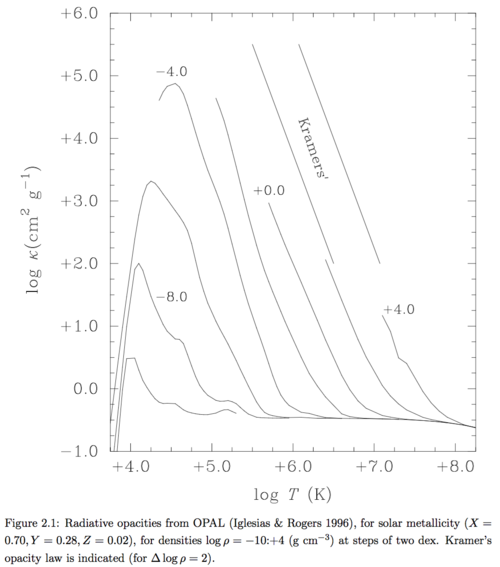
\includegraphics[width=0.75\textwidth]{figures/500px-Opacity_table.png}
    \caption{Opacity table.}
    \label{fig:opTable}
\end{figure}

The opacity dependence on temperature can be roughly broken into three temperature ranges.

\subsubsection{H- opacity}

At low temperatures $(\log T (K) \lesssim 4)$, the gas is partially but not fully ionized. Therefore free electrons can fall onto a neutral hydrogen atom forming a H$^-$ ion. The lower the temperature the less free electrons are present in the gas available to absorb photons attempting to pass through the gas. Therefore H$^-$ opacities decrease at lower temperatures. The general power law form for the H$^-$ opacity has $a = 0.5$ and $b = 9$:

$$ \kappa \propto \rho^{0.5} T^{9}$$

Notice the steep temperature dependence in this section of the opacity table.

\subsubsection{Free-free and bound-free opacity}

At higher temperatures $(4 \lesssim \log T (K) \lesssim 8)$, the gas is partially ionized with more energized electrons. Inverse Thermal Bremsstrahlung (free-free) and Milne Relation|Radiative Recombination (bound-free) are the dominate contributions to the opacity of the plasma. Both of these processes can be represented with Kramer's Opacity, which has the general power law form for the opacity with $a = 1$ and $b = -3.5$:

$$ \kappa \propto \rho T^{-3.5}$$ 

The increasing temperature of the plasma gives the free electrons enough energy to break out of the electric potential energy wells of the protons. Photons are less affected by the fast streaming electrons and as a result there is a decrease in the opacity.

\subsubsection{Thomson (electron) scattering}

At still higher temperatures $(\log T (K) \gtrsim 8)$, free electrons in the plasma will absorb and subsequently reemit incident photons via Thomson Scattering. This is a coherent scattering process (or 'grey scattering') resulting in no shift to the incident photon's energy. However the incident photon can be reemitted in a different direction, resulting in a decrease in the amount of radiation along a given line of sight. Thompson scattering is also independent of both temperature and density ($a = 0$ and $b = 0$). All values of density in the OPAL opacity table approach a constant value of $\kappa_{Th} = 0.2 (1 + X)$ where $X$ is the hydrogen mass fraction of the plasma, at sufficiently high temperatures.

Thomson Scattering is the low energy approximation of Compton Scattering, during which photons decrease in energy as they scatter off of electrons.


\subsection{Kramer's Opacity (Aaron's Notes)}

Kramers' opacity describes how the opacity of a plasma scales with density and temperature, assuming free-free absorption (Thermal Bremsstrahlung|inverse bremsstrahlung) is dominant. It is most useful for understanding and modeling stellar atmospheres.

$$\kappa_{ff} =\frac{\rho }{ T^{3.5}\,3\cdot10^{23}}\,cm^2\, g^{-1}$$

\subsubsection{Opacity due to Thermal Inverse Bremsstrahlung}

Recall that we defined the coefficient for thermal free-free absorption (Thermal Bremsstrahlung|inverse bremsstrahlung) as:
\def\knff{\kappa_{\nu,ff}}
$$\anff\equiv\frac{\jnff}{ B_{\nu}}$$
We can also define the opacity:
$$\knff=\frac{\anff}{\rho}\propto\frac{n_en_p\nu^{-3}(e^\frac{h\nu}{ kT}-1)}{
\rho\sqrt{T}e^\frac{h\nu}{ kT}}$$
where $\,\rho$ is the total density.  For a rough scaling, we can cancel the exponential terms and since most photons have an energy of order $h\nu\,\sim\, kT$, the frequency is proportional to the temperature. Setting the energy of all photons equal to the kinetic energy scale removes the frequency dependence from the opcaity and instead transforms it into a flux-weighted mean opacity.
$$\kappa_{ff}\propto\frac{n_en_p}{\rho}\frac{T^{-3}}{\sqrt{T}}$$
Additionally, typically the electron \# density is proportional to the total density, $n_e\propto\rho$, and the proton \# density is proportional to the total density times $Z$, $n_p\propto Z\cdot\rho$, so:
$$\boxed{\knff\propto\rho T^{-3.5}}$$
Including the constant of proportionality, we get:
$$\kappa_{ff}=\frac{\rho }{ T^{3.5}\,3\cdot10^{23}}\,cm^2\, g^{-1}$$
This is known as Kramer's opacity and describes the scaling of the opacity of a plasma with density and temperature assuming absorption due to Inverse Bremsstrahlung.
It is important to remember the assumptions we made to get here:
\begin{itemize}
\item A Maxwellian velocity distribution, which should be valid since the
collision time scale is very small, so the system should relax to a 
Maxwellian distribution quickly.
\item A non-relativistic regime, so $T\le\frac{m_ec^2}{ k}\sim7\cdot 10^9K$, which
is an okay assumption for most plasmas.
\end{itemize}
Some examples of Thermal Bremsstrahlung are HII regions, and the diffuse
IGM (which contains nuclei and H).

\subsection{Class Notes}

Let's discuss thermal bremsstrahlung radiation. This is a very similar concept to cooling -- the only difference is that we are not in a bound system. Before, we had QM-bound systems with discrete states. Here, we have photons produced at every level since we are in a continuum. Here, we explore this in detail. 

We must consider this where we have plasmas:
\begin{itemize}
\item Stellar Interiors
\item Stromgren spheres
\item More
\end{itemize}

Consider an electron buzzing by a nucleus. It will be re-directed by the Coulomb force, according to something like this diagram:

\begin{figure}
    \centering
    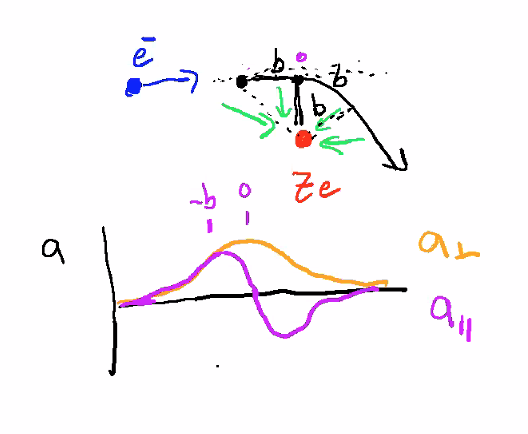
\includegraphics[width=0.75\textwidth]{figures/Screen Shot 2020-10-13 at 11.28.08 AM.png}
    \caption{Here we have the interaction and plots of the acceleration over time. We also have one acceleration along the path, and one that is perpendicular to the path. Which do we care about? Let's see below. }
    \label{fig:thermbrem}
\end{figure}

Which acceleration do we care about? We care about the acceleration that ``brakes'' the motion of the electron, converting kinetic energy to radiative energy/thermal energy. One other thing to consider -- why do we only talk about electrons? The nuclei are much more massive. And the dampening of the effect on nuclei shows up in two places: (a) in the interaction rates ($R \sim n \sigma v$) since the mass affects the velocity and (b) electrons accelerate more easily so the Larmor Power will be larger. 

So, which acceleration profile will drag on the electorn? The one parallel to its path since that is what is causing the deceleration. 

We now consider the Coulomb force between the electron and the nucleus, ignoring factors like $\sqrt2$:

$$
F \approx \frac{Ze^2}{b^2} = m)e a \rightarrow a \approx \frac{Ze^2}{b^2 m_e}
$$

We can plug this acceleration into our Larmor Power as a function of the \textbf{impact parameter} $b$:

$$
P(b) = \frac23 \frac{e^6 Z^2}{b^4 m_e^2 c^3}
$$

How do we turn this into an energy? Since the power above is ONLY when it passes by a nucleus. This power \textit{would be} true if the electrons were constantly interacting at a distance $b$. To go from power to energy, we need some timescale since $E \sim P(b) \Delta t$. Well, the acceleration profile \textit{kinda} looks like a sine wave. The peaks of the sine wave occur at roughly $45^\circ$ from the perpendicular, so we can kind of model this as equilateral triangles. This distance between these peaks is roughly $2b$, and we need to double that time. All in all, we get:

$$
T \sim \frac{4b}{v}
$$

Thus, the frequency $\nu \sim 1/T \sim \frac{v}{4b}$. As long as we are moving non-relativistically, the $\nu$ that we just calculated is the same frequency as the photon we end up producing. Thus, we can get an average power by $\langle P \rangle \sim E R_{collision}$ since this will accountfor the non-continuous interactions at a distance $b$. We KNOW the interaction rate (from above):

$$
\langle P \rangle \sim P(b) \Delta t \left(\sigma v n_e\right)
$$

Let's consider looking at a nucleus an observing what happens as electrons fly by. The electron will se a ring at a distance $b$ as the place to interact, so we have:

$$
\langle P \rangle \sim P(b) \Delta t \left(\left(2 \pi b \text{d}b\right) v n_e\right)
$$

We can divide through by $db$, getting:

$$
\frac{dP}{db} = \frac23 \frac{e^6 Z^2}{c^3 b^4 m_e^2}\frac{2b}{v} 2\pi b v n_e
$$

We don't care about the $b$ since we want to integrate over it. We ARE interested in the spectral dependence, so getting $dP/d\nu$ would be better. We have an expression for the $\nu$ and $b$ already, so we can do this! Recall that $\nu \sim v/4b$. We thus have $d\nu= \frac{-v}{4b^2}$. Substituting everythingin, we get:

$$
\frac{dP}{d\nu} = -\frac{32}{3}\frac{Z^2 e^6 n_e}{m_e^2 c^3 v}
$$

Want want a way to keep track of the velocity, so let's pick a suitable distribution: \textbf{the Maxwellian Distribution}. Note that this means we are assuming a thermal velocity distribution. Why can we do that? Well, it is ``thermal bremsstrahlung.'' Is there something other than thermal bremsstrahlung? Here's the thing --

The interactions of the electrons with the nuclei is why we have Larmor radiation, and it's also the mechanism to exchange energy and momentum. This allows us to achieve a minimum entropy distribution in velocity space, and that is the \textbf{Maxwell} distribution:

$$
f(v) = \left(\frac{m_e}{2\pi kT}\right)^{3/2} 4\pi v^2 e^{-\frac{\frac12 m_e v^2}{kT}}
$$

If we want the average power, we thus need to integrate from a minimum velocity (set by the velocity needed to bind the electron to the atom -- this is called free-to-bound transition) to infinity. What we are doing is called free-free emission: 

$$
\frac12 m_e v_{min}^2 \sim h \nu_{ionization}
$$

$$
\langle \frac{dP }{d\nu}\rangle = \int_{\sqrt{\frac{2h\nu_{ionization}}{m_e}}}^{\infty} \frac{dP}{d\nu} f(v) dv
$$

$$
\boxed{\langle \frac{dP }{d\nu}\rangle = \frac{64}{3} \sqrt{\frac{\pi}{2}} \frac{Z^2 e^6 n_e}{m_e^{3/2} c^3 \sqrt{\sqrt{kt}}}e^{-\frac{h\nu}{kT}}}
$$

We want to turn this into something that we can use, like an emissivity! There is not too much more tha we need to do -- we have taken care of all the number densities of electrons to get a power per frequency, but now we need an additional unit of inverse volume. What if we take this and mulitply by all the nuclei that are out there, including the number desnity of the protons (and considering all angles): 

$$
\jnff \sim \langle \frac{dP }{d\nu}\rangle \frac{n_{+}}{4\pi}
$$

This is mostly right, but there is one more term that comes form quantum mechanics:

$$
\jnff \sim \langle \frac{dP }{d\nu}\rangle \frac{n_{+}}{4\pi} \underbrace{\frac{\pi}{\sqrt{3}} \bar{g}_{ff}(v,T)}_\text{Gaunt factor}
$$

where the Gaunt factor is a degeneracy factor that comes from quantum mechanics. If you do stellar interiors, you definitely need this factor! Good thing is that it is often of order 1. 

$$
\jnff \sim \frac{16}{3\sqrt{2\pi}} \frac{Z^2 e^6}{m^{3/2} c^3 \sqrt{kT}} n_e n_+ e^{-\frac{h\nu}{kT}}\frac{\pi}{\sqrt{3}} \bar{g}_{ff}(v,T)
$$

One other thing to note: every process has an inverse process. If we have bremsstrahlung, we must have inverse bremsstrahlung. Inverse bremsstrahlung has to kick in to prevent us from getting infinitely bright. The nice thing is that we don't have to re-derive everthing. This is a thermal process, and in thermal processes, the source function becomes the Planck function:

$$
S_\nu = \frac{j_\nu}{\alpha_\nu} \rightarrow B_\nu = \planck 
$$

$$
\alpha_{\nu,ff} = \frac{j_{\nu,ff}}{B_{\nu}}
$$

The important scalings:

$$
\anff \propto \frac{n_e n_+ \nu^{-3}}{\sqrt{T}}
$$

If we assume that thermal and kinetic energy are roughly the same:

$$
\knff = \frac{\anff}{\rho} = \left(3 \times 10^{22} \cm^2 \g^{-1}\right) \rho T^{-3.5}
$$


%%%%%%%%%%%%%%%%%%%%%%%%%%%%%%%%%%%%%%%%%%%%%%%%%%%%%%%%%%%%%%%%%%%%%%%%%%%%%%
%%%%%%%%%%%%%%%%%%%%%%%%%%%%%%%%%%%%%%%%%%%%%%%%%%%%%%%%%%%%%%%%%%%%%%%%%%%%%%
%%%%%%%%%%%%%%%%%%%%%%%%%%%%%%%%%%%%%%%%%%%%%%%%%%%%%%%%%%%%%%%%%%%%%%%%%%%%%%
\newpage
\section{October 15, 2020: Radiative Equilibrium}

\subsection{Coulomb Focusing}

Let's talk a bit more about collisional cross sections. Consider an electron striking an atom, exciting the electron. The free electron changes kinetic energies, and the atom has an energy $h\nu$ because it has the ability to release the photon with that energy. Previously, we related the cross sections between excitation and de-excitation:

$$
g_1 v^2 \sigot(v) = g_2 v'^2 \sigto(v')
$$

Let's try to compute the cross section for excitation. It's tempting to say that the cross section is the orbital distance around the atom as a circle: $\pi a_0^2$. For hydrogen, this would be a Bohr radius. We are missing a factor here -- that factor comes from Coulomb focusing. 

In some sense, the electron is like a homing missile -- it will be attracted to the nucleus due to the charge difference. Let's introduce a new variable, $b$, which is the distance at which we can aim the electron at the atom, and still have it get deflected to a radius of $a_0$ and hit the atom. 

Let's start with angular momentum. What's the initial angular momentum? 

$$
L_i = m_e v\times v \rightarrow m_e  v b
$$

After the Coulomb focusing, we will have a different velocity due to the change in potential. This final velocity is the initial velocity plus some perpendicular velocity from the changing potential:

$$
v_f = v + v_\perp
$$

We also know that $\frac12 m_e v_\perp^2 \sim \frac{Ze^2}{a_0}$. This tells us that $v_f^2 = v^2 + \frac{Ze^2}{m_e a_0}$. We will drop the one-half to do order of magnitude. Go back to conservation of momentum:

$$
m_e v b = m_e v_f a_0 
$$

Then, 

$$
\pi b^2 = \pi a_0^2 \frac{v_f^2}{v_2}
$$

$$
\pi b^2 = \pi a_0^2 \underbrace{\left(1 + \frac{Z e^2}{m_e a_0 v^2}\right)}_\text{Coulomb focusing factor}
$$

We can now use our expression for the Bohr radius to simplify this even further (and also assuming we are at low enough velocities that we can neglect the $+1$):

$$
a_0 = \frac{\hbar^2}{Ze^2 m_e}
$$

$$
\sigot \sim \pi b^2 \sim \frac{\pi h^2}{m_e^2 v^2} 
$$

There is one more little detail -- this was a classical derivation, and we can improve this with quantum mechanical correction factors:

$$
\sigot \sim \frac{\pi \hbar^2}{m_e^2 v^2}\underbrace{\left(\frac{\Omega(1,2)}{g_1}\right)}_\text{the omega factor}
$$

$\Omega$ is called the collisional strength. It is generally 0 below some threshold velocity for this excitation interaction. It is approximately unity at the threshold for interaction, and then decreases as $v$ increases. The factor is generally of order unity, but does have a temperature dependence. 

Recall that it is useful to talk about $q_{12} = \langle \sigot v \rangle \propto \langle \frac{1}{v} \rangle \propto \frac{1}{\sqrt{T}}$. 

\subsection{Coulomb Focusing (Aaron's Notes)}

Imagine an incident electron has kinetic energy $>h\nu_{21}$.
$$\frac12 m_rv^2 \approx \frac12 m_ev^2 > h\nu_{21}$$
Coulomb focusing gives $\inv{v^2}$ cross-section.
We want to know how far away an electron with $v$ can be aimed
and still hit the $a_0$ radius cloud around the ion.  This is $b$, the
{\bf impact parameter}.  Our collision cross-section $=\pi b^2$.  Our
angular momentum is conserved, so 
$$m_ev\,b=m_ev_fa_0$$
We know that $v_f^2 = v^2 + v_\perp^2$, where $v_\perp$ is the velocity
$\perp$ to the original electron velocity.  This is a result of it falling
toward the ion.  Then:
$$\frac12 m_ev_\perp^2 \sim \frac{Ze^2}{ a_0}$$
$$v_f^2 = v^2 + \frac{Ze^2}{ m_ea_0}$$
$$b=\frac{a_0v_f}{ v}$$
$$\pi b^2 = \frac{\pi a_0^2}{ v^2}\left[v^2+\frac{Ze^2}{ m_ea_0}\right]$$
$$= \pi a_0^2\left[1+\underbrace{\frac{Ze^2}{ m_ev^2a_0}}_\text{Coulomb focusing
factor}\right]$$
Generally, the Coulomb focusing factor $>1$ because we want to excite, not
ionize.  $a_0=\frac{\hbar^2}{ Ze^2m_e}$, so:
$$\pi b^2 = \frac{\pi\hbar^2}{ m_ev^2}$$
$$\sigot = \frac{\pi\hbar^2}{ m_e^2v^2}\overbrace{\left(\frac{\Omega(1,2) }{g_1}\right)}^\text{quantum  mechanical  correction factor}$$
$\Omega$ is the ``collisional strength'', and generally is 0 below the
$v$ threshold, goes to 1 at the threshold, and decreases for increasing
$v$, with some occasional spikes.  Generally, it is of order 1, with some
slight temperature dependency.
$$\qot=\mean{\sigot v} \propto \mean{\inv{v}} \propto \inv{\sqrt{T}}$$

2000 K gas.  $v_{term} \sim \sqrt{\frac{\gamma} {kT m}}$, so 
$v\sim \sqrt{\frac{2000 }{100}}42\cdot 1\frac{km}{ s} \approx 160\frac{km}{ s}$. Then
$$\sigot \sim 10^{-14}cm^2\left(\frac{\Omega(1,2)}{ g_1}\right)$$
$$\sigot\eval{osterbrock} \sim 10^{-15} cm^2$$

\subsection{Thomson Scattering}

How do photons scattering off of charged particles? That's what we will do here! 

Consider a photon striking an elecetron. We know that the photon is actually just a plane wave in the EM field. However, for this derivation, we consider only the electric field $\Efield$. The $\Efield$-field will accelerate the electron, causing it to radiate according to the Larmor Power:

$$
P = \frac23 \frac{e^2 a^2}{c^3}
$$

We can also write down an expression for the $\Efield$ assuming the photon is propogating along $\hat x$:

$$
\vec{E} = E_0 \sin\omega t \hat z
$$

We can write down the equation of motion:

$$
m \ddot{z} = e E_0 \sin\omega t \rightarrow a_z = \frac{eE_0}{m_e}\sin \omega t
$$

We can get an rms-acceleration as a sort of average acceleration:

$$
a_{rms} = \sqrt{\langle a^2 \rangle} = \frac{e E_0}{m_e \sqrt{2}}
$$

Note that the $\sqrt{2}$ comes from the average of $\sin$ over a period. 

Solving the equation of motion:

$$
z = \int \int \frac{e E_0}{m_e} \sin \omega t = \frac{e E_0}{\omega_0^2 m_e} \sin \omega t
$$

This shows that the electron oscillates up and down on the $\Efield$. We can treat this as a dipole as it oscillates up and down

$$
\vec{p} = e d \hat{z} \rightarrow \frac{e^2 E_0}{\omega_0^2 m_e}\sin\omega t \hat{z}
$$

Oscillating electric dipoles radiate! This is a sign we are on the right track.

Let's try to find the cross section for this interaction using a nice trick. We can write down the differential power in a solid angle, and re-write it:

$$
\frac{d P }{d\Omega} = \underbrace{\frac{d P }{d\sigma}}_\text{Poynting Flux} \frac{d\sigma}{s\Omega}
$$

We have seen the Poynting flux before ($\langle s \rangle = \frac{c E_0^2}{8\pi}$. Additionally, we can cross out $d\Omega$ and integrate:

$$
P = \frac{c E_0^2}{8\pi } \sigma
$$

We can solve for $\sigma$ and plug in the Larmor Power and rms-acceleration or dipole moment from earlier. It should be noted we can rewrite the Larmor Formula in terms of the dipole moment:

$$
P = \frac23 \frac{a^2 e^2}{c^3} = \frac{d^2 \omega_0^4}{c^2}
$$

$$
\sigma = \frac{8\pi}{c E_0^2} \frac{2}{3}\frac{e^2 E_0^2}{c^3 m_e^2}
$$

$$
\boxed{\sigma = \frac{8\pi}{3} \frac{e^4}{m_e^2 c^4}}
$$

Note that the second fraction is the same as the classical electron radius. What does that even mean? Well consider setting the rest mass energy of an electron equal to the electron potential energy within some radius:

$$
m_e c^2 = \frac{e^2}{r_0 }\rightarrow r_0 = \frac{e^4}{m_e^2 c^4}
$$

All in all, we get:

$$
\boxed{\sigma_T = \frac{8\pi}{3} r_0^2 = 6.65 \times 10^{-25} \cm^{2}}
$$

What were our assumptions:
\begin{itemize}
    \item Relativistic effects -- we assumed that both $\Efield$ and the velocity of the electron were low enough. In a high $\vec{E}$ limit, we get Compton scattering! 
\end{itemize}

Let's look at some examples where this occurs. The first and foremost is in the CMB. Shortly after the Big Bang, we had primarily ionized hydrogen in the Universe. Free charged particles give us Thomson scattering, making the Universe opaque. As the Universe expanded, it cooled, and thus we get neutral hydrogen. The last photons that were scattered before this are the CMB photons! 

Slightly outside of astronomy, there are things called Tokamaks which are toroids used for fusion. There is a plasma that is heated by magnetic fields in these coils, and the power radiated is a function of electron density. If you shine a laser through the Tokamak, you can see how Thomson scattering affects the laser, giving us an idea of the electron density. 

\subsubsection{Thomson Scattering (Aaron's Notes)}

\begin{figure}
    \centering
    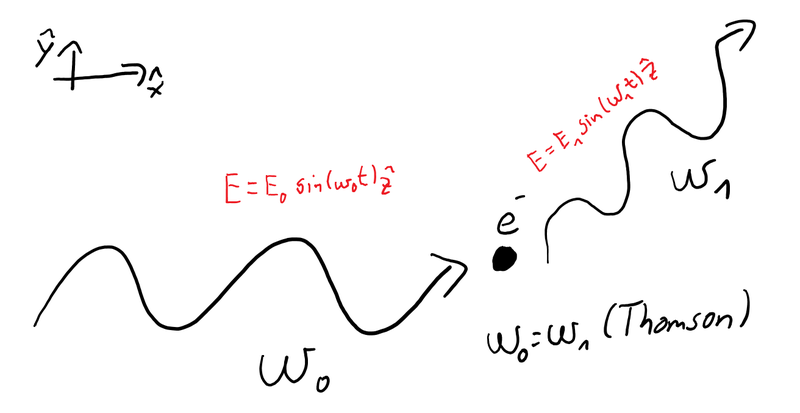
\includegraphics[width=0.75\textwidth]{figures/800px-Thomson.png}
    \caption{Thomson scattering.}
    \label{fig:thomson}
\end{figure}

Electric fields exert a force on charged particles causing them to accelerate. As seen in the derivation of the [[Larmor Formula]], accelerated charged particles emit radiation. So overall, incoming radiation might be off-scattered by charged particles. Here, we will consider incoming radiation being off-scattered by an electron, the so called Thomson scattering. Note that this requires a low energy, low intensity $\vec{E}$-field and a low energy electron. Other limits will be discussed later in the course, see [[Compton Scattering]].

An incoming electromagnetic wave with an angular frequency $\omega_0$ passes an electron of mass $m_e$. Model this wave in its easiest form by

$$E=E_0 \sin(\omega_0 t)\hat{z}.$$

The electron is accelerated by this external electric field, so that its motion is described by

$$m\ddot{z}=eE_0 \sin(\omega_0 t).$$

The root-mean-square average acceleration, which will be important for determining the radiated power is

$$a_\text{rms}=\sqrt{\langle a^2 \rangle} = \frac{eE_0}{2m_e}.$$


In order to oscillate with the same frequency as the incoming radiation, the photon energy needs to be significantly smaller than the rest energy $m_e c^2$ of the electron. This statement is equivalent saying that the wavelength of the incoming wave needs to be larger than the Compton wavelength $h/m_ec$, a characteristic scale at which quantum mechanics becomes important. At the same time, we assumed the electron to be at low velocity and the amplitude of the incoming wave to be small, otherwise a relativistic description is needed.


Integrating the equation of motion and rewriting the solution in terms of the dipole moment $d=e \cdot r$, we obtain

$$d=-d_0\sin(\omega_0 t)$$

with the dipole amplitude being $d_0=\left(\frac{e^2 E_0}{m_e\omega_0^2}\right)$.

We can use the dipole amplitude and the Larmor formula to determine the power emitted, but we need to keep track of the off-scattered direction separate of this. There will be no radiation along the dipole axis (recap the derivation of the Larmor formula if this is not obvious to you). So while there is a dependence on zenith angle $\Theta$, there is none on the azimuth angle. Therefore, a single photon does not need to continue into the direction of the incoming photon, but can be arbitrarily scattered when obeying the probability distribution resulting from the dipole field.

The differential power scattered into a solid angle $d\Omega$ as calculated in the dipole approximation is

\begin{align}
\frac{dP}{d\Omega}&=\frac{\ddot{d}^2}{4\pi c^3} \sin^2(\Theta) \\
&=\frac{e^4E_0^2}{8\pi c^3 m_e^2} \sin^2(\Theta),
\end{align}

which quantifies the statement that radiation is mostly emitted perpendicular to the moving charge and that there is no dependence on the azimuth angle.

We now try to determine the cross-section of this interaction. A trick to be used here is to expand the differential power scattered into a solid angle with $d\sigma$.

$$\frac{dP}{d\Omega}=\frac{dP}{d\sigma}\frac{d\sigma}{d\Omega}=\langle S \rangle \frac{d\sigma}{d\Omega} = \frac{cE_0^2}{8\pi}\frac{d\sigma}{d\Omega},$$

where $\langle S\rangle=\frac{dP}{d\sigma}$ is the flux passing the cross-section of the electron, which is related to the amplitude of the incoming field via the time-averaged Poynting flux.

Integrating the above equation and recalling the [[Larmor Formula]] for $P$, we obtain:

\begin{align}
\sigma_T &= \frac{8\pi}{cE_0^2} P \\
&=\frac{8\pi}{cE_0^2}\frac{e^2 a_\text{rms}^2}{3c^3} \\
&= \frac{8\pi}{3} \frac{e^4}{m_e^2c^4}=\frac{8\pi}{3} r_0^2,
\end{align}


where $r_0$ is the classical electron radius, which can be easily re-derived by requiring that the potential Coulomb energy makes up all of the electron's rest energy by bringing in charge within a radius $r_0$ that suffices this condition.

Concluding, the cross-section is off from a pure, classical cross-section for this interaction by a factor of $8/3$.

$$\sigma_T = \frac{8\pi}{3} r_0^2 = 6.65 \cdot 10^{-25} \text{cm}^2$$

\subsubsection{Examples}

\begin{figure}
    \centering
    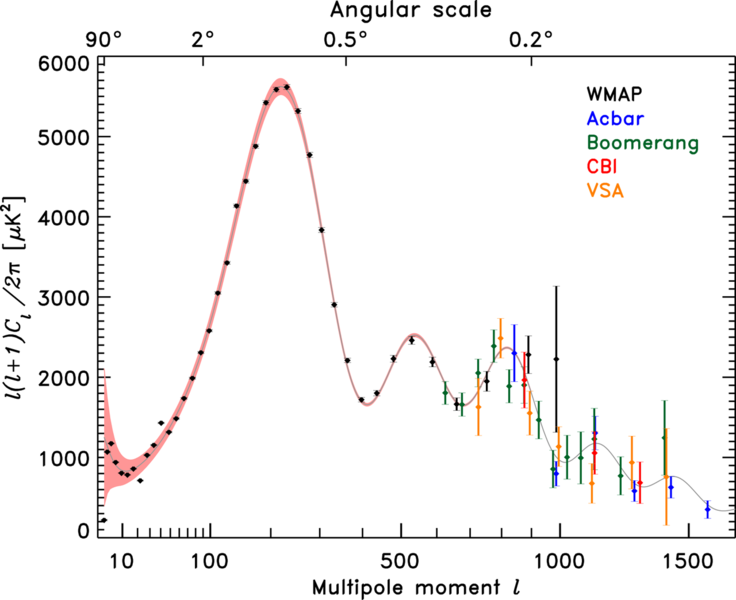
\includegraphics[width=0.75\textwidth]{figures/736px-BAO.png}
    \caption{The Power spectrum of BAO over angular scales.}
    \label{fig:BAO}
\end{figure}

Thomson scattering is important on very different scales in Astronomy. For example:

\begin{itemize}
    \item At high temperatures, Thomson scattering can dominate the photon diffusion in a star and thus determines the energy flux making its way out of the star.
    \item At the epoch of recombination ($z \approx 1100$), Thomson scattering caused the high opacity of the plasma. The effects of Thomson scattering are, for example, visible in the diffusion damping of Baryon Acoustic Oscillations. For high l-moments ($l\geq 1000$), Thomson scattering set the length over which photons could diffuse. This directly determines the damping of small scales (high moments) as inhomogeneities can be leveled out by photons.

\end{itemize}


%%%%%%%%%%%%%%%%%%%%%%%%%%%%%%%%%%%%%%%%%%%%%%%%%%%%%%%%%%%%%%%%%%%%%%%%%%%%%%
%%%%%%%%%%%%%%%%%%%%%%%%%%%%%%%%%%%%%%%%%%%%%%%%%%%%%%%%%%%%%%%%%%%%%%%%%%%%%%
%%%%%%%%%%%%%%%%%%%%%%%%%%%%%%%%%%%%%%%%%%%%%%%%%%%%%%%%%%%%%%%%%%%%%%%%%%%%%%
\newpage
\section{October 20, 2020: Milne Relation and the Saha Equation}

\subsection{Milne Relation}

\def\sigbf{\sigma_{bf}}
\def\sigfb{\sigma_{fb}}

This relates cross sections for interaction and photo-ionization interactions. Consider a photon interacting on a neutral atom. The photon ionizes the atom and sends the electron off with $E = \frac12 m_e v^2$. Some of the energy that the photon contained went into the kinetic energy, but most went into $\chi$, the ionization potential for the atom. For hydrogen, this is $\chi = 13.6 \ev$. This is a bound-free interaction, and we write the interaction cross section as $\sigbf(\nu)$ and free-bound interaction, $\sigfb(v_e)$. The Milne Relation relates these two cross sections.

A typical thing that we do when we want to relate the forward and reverse processes is to describe the rates of interaction on both sides, and then assume thermal equilibrium to relate the two rates. Let's start there. \\



\textbf{Bound-Free Transitions: Photoionization}\\

Consider $n_0$, the number of neutral atoms. If we want the number of ionizations per unit volume per unit time, we have:

$$
R = n_0 B_{bf} \bar{J}
$$

where 

$$
\bar{J} = \frac{1}{4\pi} \int I_\nu \phi(\nu) d\nu d\Omega 
$$

We want to express $B_{bf}$ as a function of $\sigbf$. We can remember that $\alpha_\nu = n_0 \sigbf$, but we have also said $\alpha_\nu = \frac{h\nu_0}{4\pi}B_{bf} n_0 \phi(\nu)$. This allows us to say:

$$
R = \int n_0 \frac{4\pi}{h\nu} \sigbf \frac{1}{\phi(\nu)} I_\nu \frac{1}{4\pi} \phi(\nu) d\nu d\Omega
$$

We also need to account for stimulated emission. For photo-excitation, we simply added the extra term for stimulated emission $-n_2 B_{21}$. We had also worked out that $g_1 B_{12} = g_2 B_{21}$. This all applies for photo-ionization as well! We can expression $B_{bf}$ in terms of the Einstein $B$'s that we know with the correction factor:

$$
1 - \frac{n_2 g_2}{n_1 g_1}
$$

Putting this in, we get:

$$
\frac{\text{no. of ionizations}}{\text{volume}\text{ time}} = \int n_0 \frac{4\pi}{h\nu} \sigbf \frac{1}{\phi(\nu)} I_\nu \frac{1}{4\pi} \phi(\nu)\left(1 - \frac{n_+ g_+}{n_0 g_0}\right) d\nu d\Omega
$$

Assuming isotropic emission, we are left with:

$$
\frac{\text{no. of ionizations}}{\text{volume}\text{ time}} = \int n_0 I_\nu 4\pi \sigbf \frac{1}{h\nu} d\nu \left(1 - \frac{n_+ g_+}{n_0 g_0}\right)
$$

Let's stop here and look at collisional recombinations:


\textbf{Free-Bound Transitions: Collisional Recombinations}\\

We can do a similar thing to above:

$$
\frac{\text{no. of recombinations}}{\text{volume}\text{ time}} = \int n_+ n_e \sigfb v f(v) dv
$$

We will now assume thermal equilibrium so that we can relate the ionizations to the recombinations, but {\textbf the Milne Relation does not depend on thermal equilibrium}. Assuming this just gives us a nice way to prove the relation. We will also assume detailed balance, so that instead of the integral numbers, we can relate only the forward and reverse reactions at every frequency. This gives us:

$$
n_0 B_\nu \frac{4\pi}{h\nu}\sigbf d\nu \left(1 - \frac{n_+ g_+}{n_0 g_0}\right) = n_+ n_e \sigfb v f(v) dv
$$

And now we can plug stuff in! Let's use the Boltzmann equation for:

$$
\frac{g_+}{g_0} = \frac{n_+}{n_0} e^{-E/kT}
$$

and for $E$ we have $E = \chi + \frac12 m_e v^2$. We can also assume a Maxwellian:

$$
f(v) = \left(\frac{m_e}{2 \pi k_b T}\right)^{3/2} 4 \pi v^2 e^{-\frac{m_e v^2}{2k_B T}}
$$

$$
B_\nu = \planck
$$

Doing some algebra and using $h\nu = E = \chi + \frac12 m_e v^2 \rightarrow h \mathrm{d}\nu = m_e v \mathrm{d} v$.

$$
\frac{n_+ n_e}{n_0}\frac{\sigfb}{\sigbf} \left(\frac{m_e}{2 \pi k_b T}\right)^{3/2} 4\pi v^3 e^{-\frac{m_e v^2}{2k_B T}} \frac{h}{m_e v} = \planck \frac{4\pi}{h\nu} \left(1 - e^{-\frac{h\nu}{kT}}\right)
$$

Lastly, we just need the Saha Equation, which relates the number density of ionized atoms and electrons to the number density of neutrals in thermal equilibrium:

$$
\frac{n_+ n_e}{n_0} = \left(\frac{2\pi m_e kT}{h^2}\right)^{3/2} \frac{2g_+}{g_0}e^{-\chi/kT}
$$

Now plugging EVERYTHING, together and simplifying:

$$
\frac{\sigfb}{\sigbf} \left(\frac{m_e^3}{h^3}\right)\frac{2g_+}{g_0}v^2 e^{-\frac{h\nu}{kT}} = \frac{2m_e \nu^2}{hc^2}\left(\frac{1-e^{-\frac{h\nu}{kT}}}{e^{\frac{h\nu}{kT}} - 1}\right)
$$

$$
\boxed{\frac{\sigfb(v)}{\sigbf(\nu)} = \frac{g_0}{g_+}\left(\frac{h\nu}{m_e c v}\right)^2}
$$

This is the {\textbf Milne Relation}. It says that the cross section to go from a free state to a bound state is related to the reverse process -- a bound to a free state as a function on frequency of the incident light -- is given by this ratio. Again, this is a general result, but we used detailed balance and thermal equilibrium to derive it. 

\subsection{Milne Relation (Aaron's Notes)}

\subsubsection{ Bound-Free Transitions (Photoionization)}

We'll calculate the cross-section of a bound-free transition $\sigbf$:
$$\sigbf\sim\frac{\lambda^2}{ 8\pi}\frac{A_{21}}{ \Delta\nu}$$
It turns out that $\Delta\nu$ is about $\nu$. $\lambda\approx 912\angstrom$, 
so scaling from Lyman-alpha:
$$\sigbf\sim\frac{(912\angstrom)^3}{ c\cdot8\pi}A_{21,Ly\alpha}
\left(\frac{1216\angstrom}{912\angstrom}\right)^3\sim 10^{-18}cm^2$$
It turns out that the real answer is $\sigbf\sim 6\cdot 10^{-18}cm^2$.  In
general:
$$\sigbf=\sigma\eval{edge}\left(\frac{E_{photon\,in}}{ E_{edge}}\right)^{-3}$$
That exponent (-3) is actually $-\frac83$ near the edge and goes to $-\frac72$
far from it.  So you see $\sigbf$ spike up as the photon reaches the 
ionization energy, and then decrease exponentially as energy increases.
However, you can see new spikes from ionizing electrons in inner shells.

\subsubsection{Radiative Recombination}

\def\sigfb{\sigma_{fb}}
This is the inverse process of photoionization, so $\sigfb$ is the cross-section
for an ion recapturing its electron and emitting a photon.  We'll relate
$\sigfb$ to $\sigbf$.  This is called the Milne Relation.  In this derivation,
we'll start by assuming complete thermal equilibrium and derive a result which
will end up being independent of thermal equilibrium.  Let's start calculating
the rate of radiative recombinations.  Thermal equilibrium dictates that this
must equal the rate of photoionization.  For radiative recombination:
$$rate\ of\ recombination
=n_+n_e\sigfb(v)v[f(v)dv]={\#\ of\ recombinations}{ volume\ time}$$
We'll set this equal to the rate of photoionization. This rate is:
$$rate\ of\ photoionization
=\frac{B_\nu4\pi d\nu}{ h\nu}n_0\sigbf
\overbrace{\left(1-\frac{g_0}{ g_+}\frac{n_+}{ n_0}\right)}^\text{correction for
stimulated recombination}$$
where $n_0$ is the \# density of neutrals. Note this has units of \# flux.
Note also that $\sigbf$ depends on $\nu$, and $\frac{n_+}{ n_0}$ is evaluated
at the relative velocity $v$ such that $h\nu=\hf m_ev^2+\chi$, where $\chi$
is the threshold ionization energy.  In thermal equilibrium, we know that (see [[Boltzmann distribution]]):
$$\frac{n_+}{ n_0}={g_+}{ g_0}e^\frac{-E}{ kT}$$
where $E$ is the energy difference between state 1 (proton + unbound $e^-$)
and state 2 (bound proton/electron pair).  Thus $E$ is given by:
$$E=\hf m_ev^2-(-\chi)=h\nu$$
So we can make our n's and g's go away.  For $f(v)$, we'll use our [[Maxwellian velocity distribution]]:
$$f(v)=4\pi\left(\frac{m_e}{ 2\pi kT}\right)^\frac{3}{ 2}v^2e^\frac{-m_ev^2}{ 2kT}$$
Finally, the [[Saha Equation]] tells us in thermal equilibrium:
$$\frac{n_+n_e}{ n_0}=\left[\frac{2\pi m_ekT}{ h^2}\right]^\frac{3}{ 2}\frac{2g_+}{ g_n}
e^\frac{-\chi}{ kT}$$
So now we're essentially done:
$$1=\frac{n_+n_ef(v)v\sigfb(v)dv}{\frac{4\pi B_\nu}{ h\nu}d\nu(1-\ehvkt)
n_0\sigbf(v)}$$
and plugging in all of our relations we get:
$$\boxed{\frac{\sigfb(v)}{\sigbf(\nu)}=
\frac{g_0}{ g_+}\left(\frac{h\nu}{ m_ecv}\right)^2}$$
\centerline{(Milne Relation)}
Notice how all of the T's vanished.  
This result is independent of thermal
equilibrium.  However, you still have to pay attention to your statistical
weights (g's).


\subsection{Saha Equation}

Photoionization is the process by which a photon knocks off an electron from an atom. The Saha equation answers the question: in thermal equilibrium, what is the ratio of atoms in a neutral state to an ionized state?

In thermal equilibrium, we typically start with the Boltzmann equation:

$$
\frac{n_1}{n_0} = \frac{g_1}{g_0} e^{-E/kT}
$$

What makes photoionzation tricky? There are a lot of different states lumped into ``ionized state'' $n_+$ since we move to a continuum state! Counting states becomes tricky, so let's simplify this to a special case. Let's consider only the ground state of a neutral atom. We also need to consider what ionization state we end up in. There's a continuum of velocities, so our Boltzmann equation becomes a differential as a function of the velocity of ejected electrons:

$$
\frac{d n_+ (v)}{n_0} = \frac{g}{g_0 }e^{-\frac{\chi + \frac12 m_e v^2}{kT}}
$$

What is $g$ here? This is the degeneracy of the ionized state. It turns out that the degeneracy of an electron is given by:

$$
g = \frac{2 \mathrm{d}V \mathrm{d}^3 p}{h^3}
$$

We also have here that $\mathrm{d}V = 1/n_e$. We also have $\mathrm{d}^3 p = 4\pi v^2 m_e^3 dv$.

\begin{figure}
    \centering
    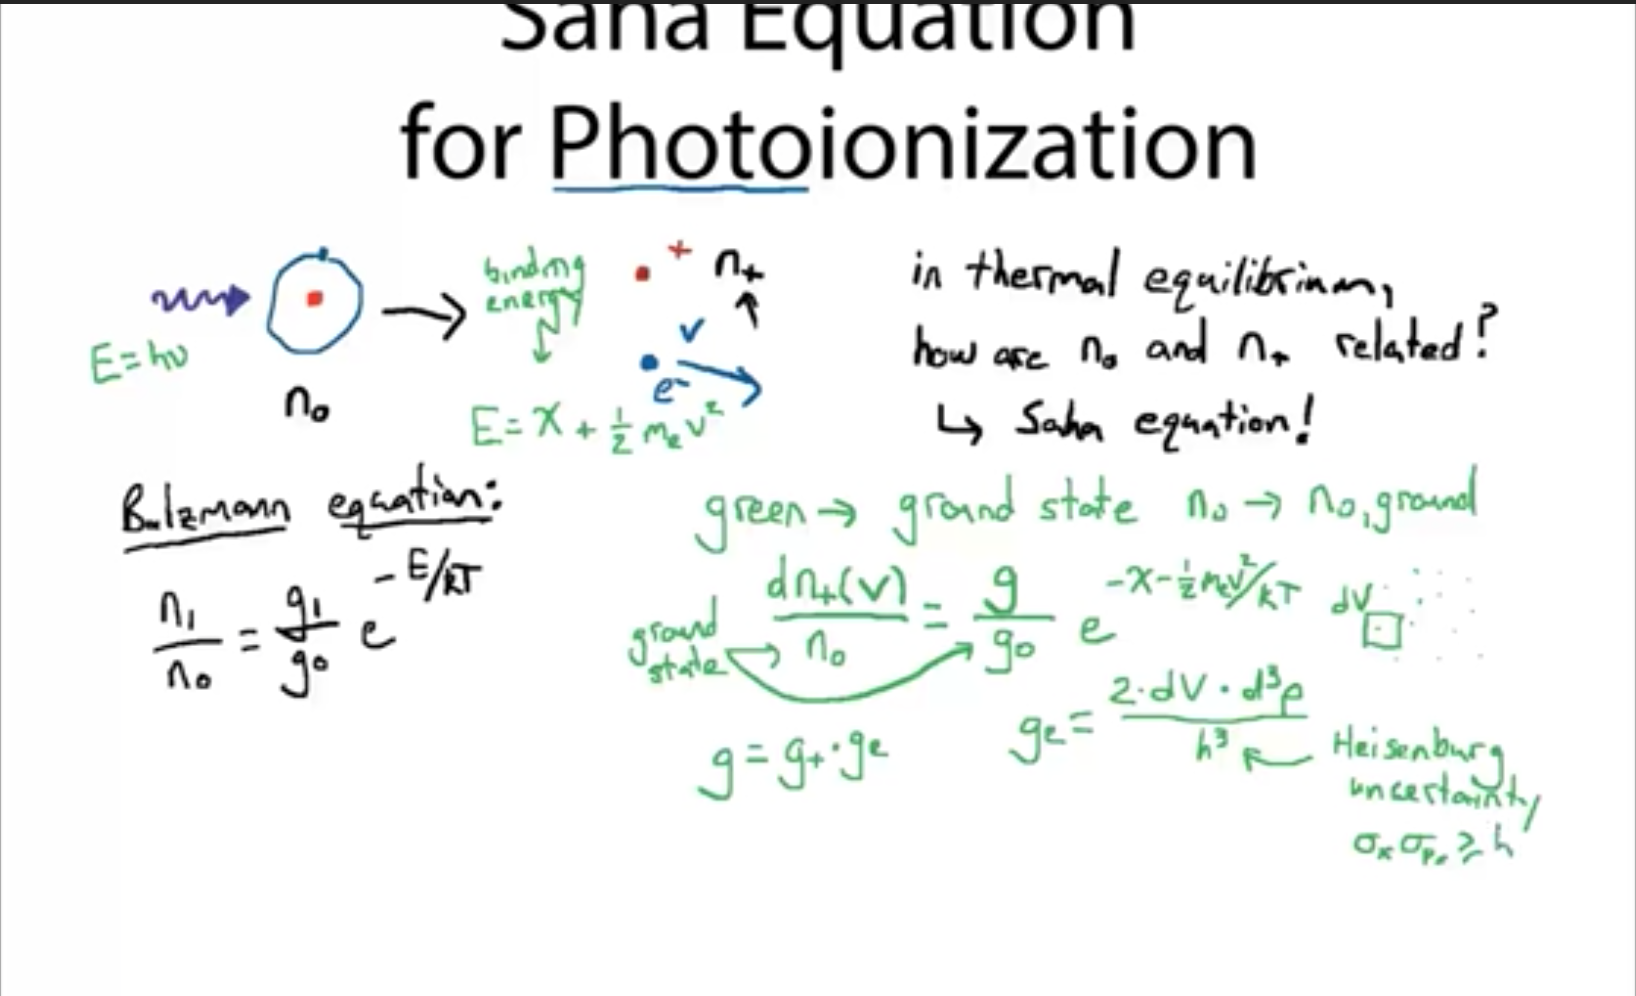
\includegraphics[width=0.75\textwidth]{figures/Screen Shot 2020-10-18 at 9.01.00 PM.png}
    \caption{Saha Equation background.}
    \label{fig:saha}
\end{figure}

Rewriting our equation:

$$
\frac{d n_+ (v)}{n_0} = \frac{8\pi m_e^3}{h^3 }\frac{g_+}{g_0 n_e }e^{-\frac{\chi + \frac12 m_e v^2}{kT}} v^2 \mathrm{d}v
$$

Remember this takes from the ground state to the velocity $v$, but we want to allow for all velocities. A change of variables $x = \sqrt{\frac{m_e}{2kt}}v$, we can integrate this:

$$
\frac{n_+}{n_0} = \frac{8\pi m_e^3}{h^3 }\frac{g_+}{g_0 n_e } e^{-\frac{\chi}{kT}} \left(\frac{2kT}{m_e}\right)^{3/2} \underbrace{\int_0^{\infty} e^{-x^2} x^2 \mathrm{d} x}_{\pi^{1/2}/4}
$$

$$
\frac{n_+ n_e}{n_0} = \left(\frac{2 \pi m_e k T}{h^2}\right)^{3/2} \frac{2g_+}{g_0}e^{-\chi/kT}
$$

This result gives us Saha's Equation for the ground state which is not the most general since this is only from the ground state. If we want to generalize to ANY excitation state, we need to translate from the ground state to any state, which is given by Boltzmann statistics:

$$
\frac{n_{0,ground}}{n} = \frac{g_0}{\underbrace{\mathcal{U}(t)}_\text{partition func.}}
$$

We also need to consider ending in any number of excitied ionization states, so we have to conisder:

$$
\frac{n_{+,ground}}{n_+} = \frac{g_+}{\underbrace{\mathcal{U}^+(t)}_\text{partition func.}}
$$

Therefore the generalized Saha equation is:

$$
\frac{n_+ n_e}{n} = \frac{2 \mathcal{U}^+(t)}{\mathcal{U}(t)} \left(\frac{2 \pi m_e k T}{h^2}\right)^{3/2} e^{-\chi/kT}
$$

How does this work in practice? Consider neutral hydrogen with $\chi = 13.6 \ev$. Naively plugging this in and seeing when the exponent is unity, we get $T = 10^{5} \K$. You then might expect recombination to have occurred at this temperature after the Big Bang! But you didn't account for the degeneracy factors. Ionized hydrogen (a single proton) has only two spin states ($\mathcal{U}^+(t) \sim 2$). Neutral hydrogen is more complicated:

$$
U \sim \sum_{i=1}^{n_{max}} g_i e^{-E_i/kT} \sim \sum_{i=1}^{n_{max}} 2 \times 2 \times (2n+1)\sim 4 n_{max}^2
$$

Therefore, the temperature at which the Universe became neutral depends on what the maximum orbital an electron going around a proton is. We know that they start out far apart, but more and more excited states lead to this infinite series of states. In practice, distant orbits lead to one in practice that depends on the temperature of the Universe. Taking $n_{max} \sim 100$, we get $\mathcal{U}(t) \sim 4 \times 10^4$. When the left side of the Saha equation is around 1, we find that $T \sim 3000 \K$ which is much more reasonable. This corresponds to a redshift of $z \sim 1100$. 


\subsection{Saha Equation (Aaron's Notes)}

\subsubsection{More on Milne }
Recall that we were deriving the [[Milne Relation]]:
$$\frac{\sigfb(v)}{\sigbf(\nu)}=\frac{g_0}{ g_+}\left(\frac{h\nu}{ m_ecv}\right)^2$$
$(\hf m_ev^2+\chi=h\nu)$.  In the following equation, Eugene has replaced
the $g_e$ of Rybicki and Lightman with the number $2$, because that is the
number of spin states of the electron.  This is just to be more clear.  So
the {\bf Saha} equation is:
$$\frac{n_+n_e}{ n_0}=\left[\frac{2\pi m_ekT}{ h^2}\right]^\frac{3}{2}\frac{2g_+}{
g_0}e^\frac{-\chi}{ kT}$$
\centerline{(Saha Equation)}
Note that the number of internal degrees of freedom for the proton $g_+=2$, and
the number for neutral hydrogen:
$$g_0=\overbrace{n^2\cdot2}^{deg\ of\ freedom\ bound\ e^-}\overbrace{\cdot2}
^{proton}$$
$$g_0=4n^2$$
Beware that Shu says $g_0=2n^2$ and $g_+=2$.  We are now going to write the
``Recombination Coefficient'' $\alpha$:
$$\begin{aligned}\alpha&=\sum{\int_0^\infty{\sigfb(n,v)v\,f(v)dv}}\\ 
&=\sum_n{\mean{\sigfb(n,v)v}}\\ \end{aligned}$$
$$\vartheta(\alpha)\simeq\vartheta\left(\sigbf(\frac{h\nu}{ m_ecv})^2v\right)$$
We'll estimate that for hydrogen, $\sigbf\sim10^{-18} cm^2$, $h\nu\approx
13.6eV$, and $v\sim\sqrt{\frac{2kT}{ m_e}}$, where $T\sim10^4K$.  Thus
$$\vartheta(\alpha)\simeq10^{-13}\frac{cm^3}{ s}\left(\frac{10^4K}{ T}\right)^\hf$$
You can look this up in Osterbrock: at $T=10^4K$, the sum over all bound
states (``recombination''):
$$\alpha_A=4\e{-13}\frac{cm^3}{ s}$$
and the sum over all bound states except $n=1$ (we might be interested in
omitting the free-to-ground transition because it is likely to ionize
a nearby atom):
$$\alpha_B=2\e{-13}\frac{cm^3}{ s}$$

\subsubsection{ Derivation of Saha}

Saha makes use of LTE.  This equation tells us what the \# density ratio is
between states 1 and 2.  We'll say that $n_{0,1}$ is the \# density of neutral
atoms with an $e^-$ in energy level 1.  $n_{+,1}$ is the \# density of ionized
atoms which still have an $e^-$ in energy level 1.  Saha says
collisional ionizations match the rate of collisional recombination:
$${n_+n_e}{ n_0}=\left[{2\pi m_ekT}{ h^2}\right]^{3}{2}{2g_+}{
g_0}e^\frac{-\chi}{ kT}$$
The [[Boltzmann distribution]] says:
\def\npo{n_{+,1}}
\def\noo{n_{0,1}}
\def\gpo{g_{+,1}}
\def\goo{g_{0,1}}
$$\frac{\npo}{\noo}=\frac{\gpo}{\goo}e^\frac{-E}{ kT}$$
where $E=E_{state\ 2}-E_{state\ 1}=\hf m_ev^2-(-\chi)=\hf m_ev^2+\chi$.  Now
we need to figure out our numbers of internal degrees of freedom:
$$\gpo =\gpo\eval{internal}\cdot g_e\eval{internal}\cdot 
g_e\eval{translational\ motion}\cdot \gpo\eval{translational\ motion}$$
$g_e$ is easy: $g_e=2$.  $g_e\eval{translational}$ is harder:
$$g_e\eval{translational} = {(vol\ in\ conf\ space)(vol\ in\ momentum\ space)
}{ h^3}$$
The volume in configuration space is $\inv{n_e}$.  The volume in momentum
space is $4\pi p^2dp=4\pi m_e^3v^2dv$. Now on to $\goo$:
$$\goo=\goo\eval{internal}\cdot\goo\eval{translational}$$
$$\frac{\npo}{\noo}=\int_0^\infty{\gpo\eval{internal}\cdot\gpo\eval{trans}
}{\goo\eval{internal}\cdot\goo\eval{trans}}\frac{2}{ n_e}
\frac{4\pi m_ev^2dv}{ h^3}e^\frac{-(\hf m_ev^2+\chi_1)}{ kT}$$
$$\frac{\npo n_e}{ \noo}=\left[\frac{2\pi m_ekT}{ h^2}\right]^\frac{3}{2}
\frac{2\gpo\eval{int}}{\goo\eval{int}}e^\frac{-\chi_1}{ kT}$$
Now what if we were talking about going from neutral bound state in energy
level 2 (instead of 1) to an ionized atom with electron in energy state 1.
It turns out, we just need to replace $\goo$ with $g_{0,2}$ and
\def\got{g_{0,2}}
\def\nzt{n_{0,2}}
$\chi_1$ with $\chi_2=\chi_1-E_{0,12}$.  Thus:
$$\frac{\npo n_e}{\nzt}=\left[\frac{2\pi m_ekT}{ h^2}\right]^\frac{3}{2}\frac{2\gpo
e^\frac{-\chi_2}{ kT}}{\got e^{E_{0,12}}{ kT}}$$
\def\tpmekth{\left[\frac{2\pi m_ekT}{ h^2}\right]^\frac{3}{2}}
Where the rightmost, bottom factor used to be $\goo$.  In general,
$$\frac{n_{0,j}}{ t_je^\frac{-E_{0,1j}}{ kT}}=\frac{\npo n_e}{\tpmekth 2\gpo
e^\frac{-\chi_1}{ kT}}$$
We'll define the right-hand side above to be $R$.  Then:
$$\frac{R}{ n_0}=\inv{U_0(T)}=\frac{\npo n_e}{\tpmekth 2\gpo
e^\frac{-\chi_1}{ kT}n_0}$$
$$\frac{\npo n_e}{ n_0}=\tpmekth\frac{2\gpo}{ U_0(T)}
e^\frac{-\chi_1}{ kT}$$
$$\boxed{\frac{n_pn_e}{ n_o}=\tpmekth\frac{2U_+(T)}{ U_0(T)}
e^\frac{-\chi_1}{ kT}}$$
This is the full Saha equation.  Remember that Saha assumes that we are in LTE:
the rate of collisional ionizations must equal the rate of collisional 
recombination.  This predicts why we had to wait until the
universe got to 3000K until recombination occurred.  We would have naively 
expected
that as soon as the temperature of the universe dropped below the ionizing 
energy of ground-state hydrogen, we would have recombination.  However, 
Remember that we can't follow Saha out too far.  Soon, collisions stop happening
often enough to maintain LTE, and Saha becomes invalid.  For example, Saha
would say that after recombination we would continue to lose free electrons
at the same (logarithmic) rate.  In truth, the number of free electrons
asymptotically approaches $10^{-3}n_B$ (where $n_B$ is the number of baryons).
We can estimate why this is.  The time for a proton to find an electron is
given by:
$$t=\inv{n_e\mean{\sigfb v}}\ll\frac{a}{ \dot a}$$
That is, collisional ionizing equilibrium just starts to fail when:
$$\inv{n_e\mean{\sigfb v}}\sim\frac{a}{ \dot a}$$
Since we know the Hubble time ($2\e5 yrs$), we can actually estimate
the number of free electrons in the universe at the time of recombination:
$$n_e\sim\inv{(2\e{-13})(2\e5)(\pi\e7)}\sim1$$



\subsection{Class Notes}

We introduced collisional excitations (usually iwth electrons), and those can excite different transitions in the atom. We can also collide atoms to atoms, if you want; and don't forget that these can all be aided by charged particles. We also have a host of coefficients to deal with for all processes -- the forward and reverse for each.

Today, we treat the ionization cases -- the combination of charge particle interactions and photon interactions. This leads to the Milne Relation and the Saha Equation. Consider these interactions (which are time reversed of each other): 

\begin{figure}
    \centering
    \includegraphics[width=0.75\textwidth]{figures/Screen Shot 2020-10-20 at 11.16.37 AM.png}
    \caption{The Saha Equation motivation.}
    \label{fig:saha_mot}
\end{figure}

Consider hydrogen -- $\chi = 13.6 \ev$ which is an ultraviolet photon, so to ionize hydrogen, we need quite hot stars like O and B types to heavily ionize the hydrogen. The language we use for these interactions are ``bound-free'' transitions and ``free-bound'' transitions, with cross sections $\sigbf$ and $\sigfb$, respectively. The forward interaction is called photo-ionization. The reverse is called recombination. Qualitatively, the former has a photon coming in, striking an electron, and sending it off with a kinetic energy. The latter involves an electron passing close to a proton, recombining, and emitting a photon. 

A reasonable thing we might ask -- consider a number density of nuclei, a number density of electrons, and a number density of neutral atoms -- what is the equilibrium state of this configuration? 

We can make this question manageable by asssuming \textbf{local thermodynamic equilibrium}. This allows us to ask how $n_e$ and $n_+$ relate to $n_0$. The equation that relates all of these is the \textbf{Saha Equation}. In some ways, this is a special case of the Boltzmann equation:

$$
\frac{n_2}{n_1} = \frac{g_2}{g_1} e^{-E/kT}
$$

We are going to take this equation and re-purpose it for ionization. As you might guess, when we assume LTE, we are allowing ourselves to use some things: the Boltzmann equation, and that our intensity goes to the Planck Function. Also, we generally assume Maxwell-Boltzmann distribution. 

Here's the recipe, specifically, for the Saha Equation: 
\begin{itemize}
    \item Assume LTE.
    \item Start with Boltzmann equation.
    \item Find relative population of ionized vs. neutral atoms. 
\end{itemize}

Things are complicated because there are a lot of ways to be in the $n_0$ state. The trick? Let's assume, for now, that $n_0$ is the ground state. In reality, the electron could be in a non-ground state and then get ionized. But for now, we will assume $n_0$ is the ground state. It's also true that there are a ton of ionized states -- in fact, there is a continuum of states! So we need the probability of jumping to a specific velocity state of the electron -- we will then assume that $n_+ = \int \mathrm{d}n_+(v) \mathrm{d}v$. We could get $\mathrm{d}n_+(v)$ from Boltzmann:

$$
\frac{\mathrm{d}n_+(v)}{n_0} = \frac{g_+(v)}{g_0} e^{-\frac{\chi + \frac12 m_e v^2}{kT}}
$$

And that's it! From here on out, it's just about calculating degeneracies...but that is tricky because we have a continuum of states that the electron can be in. 

Let's start by figuring out $g_+(v)$. Consider a proton and an electron which can both have spin states: $g_+(v) = g_{+,spin} \underbrace{g_{e,spin}}_{2} (\text{all momenta}) \rightarrow g_{+,spin} g_{e,spin} \frac{\mathrm{d}V\mathrm{d}^3p}{h^3}$ where the momenta comes from Heisenberg's Uncertainity Principle. 

We can get the quantities for all momenta from dimensional arguments -- $\mathrm{d}V = \frac{1}{n_e}$, $\mathrm{d}^3p = 4\pi^2 v^2 \mathrm{d} v m_e^3$.

We can start plugging all of this into our modified Boltzmann equation:

$$
\frac{\mathrm{d}n_+(v)}{n_0} = \frac{8\pi m_e^3}{h^3} \frac{g_+ }{n_e g_0 }v^2 \mathrm{d}v e^{\frac{-\chi - \frac12 m_e v^2}{kT}}
$$

From here, we need to integrate $\mathrm{d}n_+(v) \mathrm{d}v$. This is a messy integral, be forewarned:

$$
\frac{n_+}{n_0} = \int \frac{\mathrm{d}n_+}{n_0}\mathrm{d}v
$$

Letting $x=\sqrt{\frac{m_e}{2kT}}v$, we get:

$$
\frac{n_+}{n_0} =  \frac{8\pi m_e^3}{h^3} \frac{g_+}{n_e g_0} e^{-\frac{\chi}{ kT}} \left(\frac{2kT}{m_e}\right)^{3/2}\int_0^{\infty} e^{-x^2} x^2 \mathrm{d}x
$$

The integral has a closed form of $\sqrt{\pi}/4$. We then get:

$$
\frac{n_+ n_e}{n_0} = \left(\frac{2\pi m_e kT}{h^2}\right)^{3/2} \frac{2g_+}{g_0} e^{\frac{-\chi}{kT}}
$$

This is sometimes called the Saha equation, but remember that we assumed that $n_0$ was already in the ground state. We need to modify this for the non-ground state case, but often the above equation works. 

If you want the full derivation, we need to deal with the fact that $\frac{n_{0,ground}}{n_0} = \frac{g_0}{\mathcal{U}(T)}$. The degeneracy is temperature dependent because certain energy levels cannot be accessed without a minimum temperature. The true degeneracy is a weighted average of the degeneracies of the states in which the population is. 

$$
g_{total} = \sum g_i w_i\left(T\right)
$$

where the $w_i$'s are the weights calculated from the relative populations in state with degeneracy $g_i$. 

You then need to substitute in the partition functions for the more general expression:

$$
\boxed{\frac{n_+ n_e}{n} = \left(\frac{2\pi m_e kT}{h^2}\right)^{3/2} \frac{2\mathcal{U}_+(T)}{\mathcal{U}(T)} e^{\frac{-\chi}{kT}}}
$$

This is the \textbf{Saha equation}. Remember these ingredients: the Boltzmann distribution and then the degeneracies of electrons. We also assumed local thermodynamic equilibrium.

\par\noindent\rule{\textwidth}{0.4pt}

Now, we want to take this to a situation with limited ionizing photons. The standard way we dealt with this was turning them into cross sections and balancing \textbf{rates}. How do we obtain a cross section for these interactions? Well for photo-absorption:

$$
\sigbf(\nu) = \sigma_{edge}(\nu_0) \left(\frac{\nu}{\nu_0}\right)^{-3}
$$

But for free-bound transitions, this is much more complicated. We call what we are about to launch into \textbf{the Milne Relation} -- it calculates a bound-free transition cross section as a function of frequency and how it related to a free-bound state as a function of velocity:

$$
\sigbf(\nu) \iff \sigfb(v)
$$

Let's first talk about bound-free transitions. The picture, as before -- a photon comes in, strikes an electron sitting in an ionization potential, and we transition to a proton sitting and an electron flying off with a kinetic energy. 

$$
\frac{\text{no. of ionizations}}{\text{volume} \text{ time}} = n_0 B_{bf} \bar{J} 
$$

where $B_{bf}$ is the Einstein coefficient, and

$$
\bar{J} = \frac{1}{4\pi} \int I_\nu \phi(\nu) \mathrm{d}\nu \mathrm{d}\Omega
$$

Now, we want to turn this into something with a cross section. We've done something similar before by saying $\alpha = n_0 \sigbf$. We then asked for the units of $\alpha I_\nu$ which gave us an inverse volume. We then tried to cook-up ways of building this out from fundamental things:

$$
\alpha I_\nu = \frac{h\nu}{4\pi} \phi(\nu) n_0 B_{bf} \bar{J}
$$

We can cancel the two specific intensities, giving an expression for $\alpha$. Next, we say $\alpha = n_0 \sigbf$. We thus get:

$$
\sigbf (\nu) = \frac{h\nu}{4\pi} \phi(\nu)  B_{bf}
$$

Returning to our ionizations per volume per time, we get:

$$
\frac{\text{no. of ionizations}}{\text{volume} \text{ time}} = n_0 \frac{h\nu}{4\pi} \frac{1}{\phi(\nu)}  \sigbf \frac{1}{4\pi} I_\nu \phi(\nu) \mathrm{d}\nu \mathrm{d}\Omega
$$

This is almost right when we integrate, but we need to account for the reverse process (stimulated emission). Before, we did this by $n_1 B_{12} \rightarrow n_1 B_{12} - n_2 B_{21}$. We also had $g_1 B_{12} = g_2 B_{21}$. Both of these have their analogs in the case we care about. The actual result is that:

$$
n_1 B_{12} \underbrace{\left(1 - \frac{n_2 B_{21}}{n_1 B_{12}}\right)}_\text{correction factor}
$$

This means:

$$
B_{bf} \rightarrow B_{bf}\left(1 - \frac{n_+ g_{0}}{n_0 g_+}\right)
$$

Giving:

$$
\frac{\text{no. of ionizations}}{\text{volume} \text{ time}} = \int n_0 \frac{h\nu}{4\pi}  \sigbf  I_\nu \left(1 - \frac{n_+ g_{0}}{n_0 g_+}\right) \mathrm{d}\nu \mathrm{d}\Omega
$$

We now need to do the same thing but for free-bound transitions! We need:

$$
\frac{\text{no. of recombinations}}{\text{volume} \text{ time}} 
$$

which we can then ask to balance out with the ionizations rate we had earlier. This one is not as tricky:

$$
\frac{\text{no. of recombinations}}{\text{volume} \text{ time}} = \int n_+ n_e \sigfb v_{rel} f(v) \mathrm{d}v
$$

This looks just like collisional excitations which were not too bad. 

Setting the two rates equal (assuming equilibrium):

$$
\frac{\text{no. of recombinations}}{\text{volume} \text{ time}} = \frac{\text{no. of ionzations}}{\text{volume} \text{ time}}
$$

We will pull a trick -- let's assume that the cross sections are intrinsic, and then must hold for all cases. One of those cases is local thermodynamic equilibrium! We will then \textbf{use LTE to solve for} $\frac{\sigfb}{\sigbf}$, though this result \textbf{does not depend on LTE}.

Here is where we go crazy, off-the-rails with algebra! We will use the following things:

\textbf{From conservation of energy:}
$$
E = \chi + \frac12 m_e v^2 = h\nu
$$

\textbf{The derivative of conservation of energy:}
$$
m_e v \mathrm{d}v = h \mathrm{d} \nu
$$

\textbf{The Boltzmann Equation:}
$$
\frac{n_+}{n_0} = \frac{g_+}{g_0} e^{-E/kt}
$$

\textbf{A Maxwellian:}
$$
f(v) = \left(\frac{m_e}{2\pi kT}\right)^{3/2} 4 \pi v^2 e^{-\frac{\frac12 m_e v^2}{kT}}
$$

\textbf{Planck Function:}
$$
B_\nu = \planck
$$

\textbf{The Saha Equation:}
$$
\frac{n_e n_+}{n_0} = \left(\frac{2\pi m_e kT}{h^2}\right)^{3/2} e^{-\chi/kT}
$$

\textbf{Detailed Balance:}
We can remove the integrals from the expressions for rates per volume per time since detailed balance equations \textbf{all} forward with reverse processes. Using all of the above:

$$
\frac{n_+ n_e}{n_0} \frac{\sigfb}{\sigbf} \left(\frac{m_e}{2\pi kT}\right)^{3/2} 4 \pi v^3 \frac{h}{m_e v} e^{-\frac{\frac12 m_e v^2}{kT}} = \planck \frac{4\pi}{h \nu} \left(1 - e^{\frac{-h\nu}{kT}}\right)
$$

We then plug in the Saha Equation for $\frac{n_e n_+}{n_0}$.

$$
\frac{\sigfb}{\sigbf} \left(\frac{2\pi m_e kT}{h^2}\right)^{3/2} \frac{2g_+}{g_0} e^{-\chi/kT} \left(\frac{m_e}{2\pi kT}\right)^{3/2} v^2 e^{-\frac{\frac12 m_e v^2}{kT}} = \frac{2m_e \nu^2}{hc^2} \left(\frac{1-e^{-\frac{h\nu}{kT}}}{e^{\frac{h\nu}{kT}} - 1}\right)
$$

All of the exponentials die since you have energies as arguments which are the photon energy! We thus get:

$$
\boxed{\frac{\sigfb(v)}{\sigbf(\nu)} = \frac{g_0}{g_+}\left(\frac{h\nu}{m_e  c v}\right)^{2}}
$$

This is a general result and does not rely on thermodynamic equilibrium. 




%%%%%%%%%%%%%%%%%%%%%%%%%%%%%%%%%%%%%%%%%%%%%%%%%%%%%%%%%%%%%%%%%%%%%%%%%%%%%%
%%%%%%%%%%%%%%%%%%%%%%%%%%%%%%%%%%%%%%%%%%%%%%%%%%%%%%%%%%%%%%%%%%%%%%%%%%%%%%
%%%%%%%%%%%%%%%%%%%%%%%%%%%%%%%%%%%%%%%%%%%%%%%%%%%%%%%%%%%%%%%%%%%%%%%%%%%%%%
\newpage
\section{October 22, 2020}

\subsection{Recombination Coefficients (Aaron's Notes)}

\subsubsection{Derivation}

\def\sigbf{\sigma_{bf}}
\def\alphaNL{\alpha_{n,l}}
\def\sigfb{\sigma_{fb}}

The recombination coefficient $\alphaNL$ is analogous to $q_{12}$, the collisional rate coefficient, and is derived in a similar way. The rate of recombinations per unit volume is:

$$\frac{\textrm{\#\ of\ recombinations}}{ \textrm{volume} \cdot \textrm{time} }= n_+n_e\mean{\sigfb v} = n_+n_e\int_0^{\infty}\sigfb(v)v f(v)dv = n_+n_e \alphaNL$$
Therefore the recombination coefficient for recombination to level \emph{n, l} (\emph{n} is the principal quantum number and \emph{l} is the orbital quantum number) is defined below where $f(v)$, the distribution of velocities, is a Maxwellian.  
$$\alphaNL \equiv \int_0^{\infty}\sigfb(v)v f(v)dv = 4\pi \int_0^{\infty}\sigfb(v) \left(\frac{m}{ 2 \pi kT} \right)^{3/2} v^3 \exp\left(-\frac{mv^2}{2kT}\right) dv$$

To find how $\alphaNL$ scales with temperature, it is necessary to track all the factors of $\textrm{v}$ and $T$ in the expression above. Since recombination involves positively charged ions and electrons, $\sigfb$ accounts for Coulomb Focusing and scales as $\textrm{v}^{-2}$. It follows that $\alphaNL \propto T^{-1/2}$. For Hydrogen-like ions with nuclear charge $Z$, $\alphaNL \propto Z \cdot T^{-1/2}$.

A Hydrogen atom can recombine directly into the ground state or first to an excited state before the electron cascades down to the ground state. To account for all the ways to recombine to the ground state ($n=1$, $l=0$ or $1s$ state), the total recombination coefficient $\alpha_A$ with units $\textrm{cm}^3 \textrm{s}^{-1}$ is
$$ \alpha_A = \sum_{n=1} \sum_{l=0}^{n-1} \alphaNL$$
As will be discussed below, however, sometimes we want to omit free-to-ground transitions which are recombinations that are direct into the ground state. For these cases we use $\alpha_B$:
$$ \alpha_B = \sum_{n=2} \sum_{l=0}^{n-1} \alphaNL$$

\subsection*{Back of the Envelope Approximation and True Values}
For Hydrogen, the rate of recombination per unit volume is approximately equal to the probability of finding an electron and proton ''near'' one another in 3-dimensional space multiplied by the rate of an electron decaying from a free to a bound state. For an electron and proton to be about a few Bohr radii apart, their proximity traces out a volume $\sim 10^{-23} \textrm{cm}^3$. The atomic decay rate is $\sim 10^9 \textrm{s}^{-1}$. Let's include an extra order of magnitude because of coulomb focusing. Multiplying these together, we would predict that $\alpha_A \sim 10^{-13} \textrm{cm}^3 \textrm{s}^{-1}$ which is quite close to Hydrogen's recombination coefficients at $T=10^4 \textrm{K}$, a typical nebula temperature:

$$\alpha_A=4\e{-13}\frac{cm^3}{ s}$$
$$\alpha_B=2\e{-13}\frac{cm^3}{ s}$$

\subsubsection{Timescales}
For a typical nebula at $T=10^4 \textrm{K}$, the recombination time is:
$$t_{rec} \approx \frac{1 }{ n_e * \alpha_A} \approx 3 \times 10^{12} n_e^{-1} \textrm{sec} \approx 10^{5} n_e^{-1} \textrm{yrs} $$

The recombination time is longer than the timescales of the other relevant processes, namely photoionization and electron-electron scattering/collisions. This is good verification that it was appropriate to use a Maxwellian distribution of velocities in the derivation above. After being photoionized, the electrons thermalize so their velocities settle into a Maxwellian on timescales shorter than those associated with recombination or ionization. (The $e^--e^-$ cross-section is larger than the photoionization cross-section by several orders of magnitude.)

\subsubsection{Case A and B Recombination}
For optically thin nebulae, $\alpha_A$ is appropriate and we include recombinations that go directly from free to the ground bound state. But when a nebula is optically thick, no ionizing photons ($h \nu > 13.6 eV$ for an H nebula) escape the nebula--each photoionizing photon released from a direct free-to-ground recombination immediately photoionizes a neutral Hydrogen atom nearby, having no impact on the net recombination. In this case we want to ignore free-to-ground recombination when determining the equilibrium between photoionization and recombination. The appropriate recombination coefficient is $\alpha_B$.


Instead of recombining directly to the \emph{ground state}, sometimes a proton and an electron can recombine to form Hydrogen in an \emph{excited state} followed by a cascading down to lower energy levels. This process releases multiple lower-energy photons that are not able to subsequently photoionize other bound Hydrogen atoms because they have $h \nu < 13.6 eV$. Essentially one photoionizing photon (the one that produced the proton-electron pair in quesion) is ''exchanged for'' several lower-energy photons. Eventually as you get further away from the source of the photoionizing photons, the Hydrogen nebula will be entirely neutral because this ''exchange'' occured enough times that no photoionizing photons remain. This is the premise of Str\"{o}mgren spheres--bubbles of fully ionized Hydrogen that form around young Type O and B stars in nebulae of neutral hydrogen. These bubbles have definitive radii and thin edges, where the edge is the boundary between the fully ionized and fully neutral Hydrogen regions.

\subsection{Review of Equilibria}

We have talked about a lot of ways of exciting atoms -- photo-excitations, photo-ionizations, free-free emission, collisional-excitation -- all of which can contribute to an equilibrium. Of course, we also have the inverse processes, like emission, recombination, inverse free-free (inverse bremsstrahlung), collisional de-excitation. 

Ultimately, equilibrium is in the equating of these processeses.

\newcommand{\maxwellian}{\left(\frac{m}{2\pi k T}\right)^{3/2} 4 \pi v^2 e^{-\frac{m v^2}{2 k T}}}

\begin{figure}
    \centering
    \includegraphics[width=0.75\textwidth]{figures/Screen Shot 2020-10-19 at 12.13.06 AM.png}
    \caption{Name that equilibrium questions!}
    \label{fig:equil}
\end{figure}

\begin{itemize}
    \item Question 1: In statistical equilibrium, what describes the ratio of states in a neutral atom?
    \begin{itemize}
        \item Boltzmann Equation:
        \begin{equation}
            \frac{n_2}{n_1} = \frac{g_2}{g_1} e^{-\frac{\Delta E}{k_B T}}
        \end{equation}
    \end{itemize}
    \item Question 2: Which processes contribute to statistical equilibrium? 
    \begin{itemize}
        \item Photo-excitations because the presence of photons can affect the ratio of excited to de-excited states. We also have collisional excitations, so if we collide often, that can have an effect. 
        \item How do we determine which is dominant? We need to compare the rates of excitation and de-excitation. A quick rule of thumb is to compare $A_{21}$ (rate of de-excitation proxy) to the rate of collisions $\langle n_{e} \sigma v_{rel} \rangle$ where we average of a velocity distribution (Maxwellian in thermal equilibrium). 
    \end{itemize}
    \item Question 3: Why is it it a Maxwellian? And what is it?
    \begin{itemize}
        \item Mathematically:
        \begin{equation}
            f(v) = \overbrace{\left(\frac{m}{2\pi k T}\right)^{3/2}}^\text{normalization} \overbrace{4 \pi v^2}^\text{velocity surface} \underbrace{e^{-\frac{m v^2}{2 k T}}}_\text{energy weight}
        \end{equation}
        \item In some ways, the Maxwellian is a special case of Boltzmann statistics. 
        \item How do we get a Maxwellian? With collisions! Which processes are likely to contribute to achieving a Maxwellian distribtion?
        \begin{itemize}
            \item Collisional excitations
            \item Free-free emission
            \item Any interaction between charged or neutral particles will re-distribute energy to a Maxwellian
        \end{itemize}
    \end{itemize}
    \item Question 4: What equation governs photo-ionization? The Saha Equation!
    \begin{equation}
        \frac{n_+ n_e}{n_0} = \frac{2 \mathcal{U}^+(T)}{\mathcal{U}(T)}\left(\frac{2\pi m_e kT}{h^2}\right)^{3/2}e^{-\frac{\chi}{kT}}
    \end{equation}
    \begin{itemize}
        \item The partition functions $\mathcal{U}(T)$ are essentially degeneracies for the ions or neutral atoms -- how many different ways can you have a neutron vs. ion atom? 
    \end{itemize}
    \item Question 5: For many photon absorption by a medium, what is the equilibrium spectrum that you achieve? A Planck Spectrum/Blackbody!
    \begin{equation}
        B_\nu = \planck
    \end{equation}
    \item Question 6: How many different temperatures are there? And how are they coupled?
    \begin{itemize}
    \item See Equilibria Triangle for coupling
        \item Brightness Temperature -- Describes the photon distribution. 
        \item Excitation Temperature -- Describes the ratio of internal energy states (i.e., excited vs. de-excited atoms, or ions to neutrals)
        \item Kinetic Temperature -- Describes the distribution of velocities
    \end{itemize}
    \item Question 7: What are the conditions for local thermodynamic equilibrium?
    \begin{equation}
        T_K = T_{ex} = T_b
    \end{equation}
    \begin{itemize}
        \item What do we mean by ``local?''
        \begin{itemize}
            \item Spatially local
            \item Spectrally local
        \end{itemize}
    \end{itemize}
    \item Question 8: Can we describe an equilibrium that relates different frequencies?
    \begin{itemize}
        \item Bolometric Equilibrium:
        \begin{itemize}
            \item Consider some photons striking dust and being absorbed. This dust will re-radiate in the infrared as it heats up. Bolomoetric equilibrium happens when:
            \begin{equation}
                \sigma T^4 = \int I_\nu \phi(\nu) d\Omega d\nu
            \end{equation}
            \item In bolometric equilibrium, the total energy is conserved, but the energy is being absorbed and emitted at different frequencies. 
        \end{itemize}
    \end{itemize}
\end{itemize}

\subsection{Review of Equilibria (Aaron's Notes)}

\subsubsection{Equilibria Triangle}
Particles in an ensemble over time equilibrate into a steady state, which can be described by various distributions. The resulting ensemble of particles is dependent on temperature, where this temperature which may differ between the various equilibria. The following list describes the main equilibria for: 

\begin{itemize} 
\item $T_B$ The brightness temperature describes the energy distribution of particles as a function of frequency 
\item $T_*$ The excitation temperature controls the number density of particles in the various excitation levels 
\item $T_K$ The kinetic temperature controls the velocity distribution of an ensemble of particles 
\end{itemize} 


\begin{figure}
    \centering
    \includegraphics[width = 0.8\textwidth]{figures/800px-EquilibriaTriangle.png}
    \caption{Thermodynamic Equilibrium Triangle}
    \label{fig:triangle}
\end{figure}


\subsubsection{Statistical equilibrium}
Starting in the bottom right of the triangle, we have the $T_*$.
\begin{equation} 
\frac{n_2}{n_1} = \frac{g_2}{g_1} e^{-\Delta E/kT_*}
\end{equation}

 The [[Boltzmann distribution]] describes the most probable number density distribution for various excitation levels, as a function of the degeneracies of the states and the excitation temperature. Whereas the number of degeneracies increases at higher states ($g \sim \tilde{n}^2$), the energy required for transition increases as well, causing the distribution to peak at intermediate state,$\tilde{n}$. The exact peak can be calculated by differentiating the Boltzmann distribution with respect to the state number 

\begin{equation} 
\tilde{n}_{max} \sim \sqrt{\frac{kT}{2\hbar}}
\end{equation}

\subsubsection{Planck distribution}
For a perfect black-body, the energy distribution (spectrum) of the emitted particles is described by Planck's equation (see [[Black-Body Radiation]]). This distribution determines the energy distribution of particles as a function of frequency for a given brightness temperature, $T_B$ ( top of the triangle). 

\begin{equation} 
I_\nu = \frac{2h\nu^3}{c^2} \frac{1}{e^{h\nu}{kT_B}-1}
\end{equation}

The term brightness temperature is often used in radio astronomy in the Rayleigh-Jeans limit ($h\nu<<kT_B$)  to express the flux from an object in units of K. 

\begin{equation} 
I_\nu = \frac{2kT_B}{\lambda^2}
\end{equation}


\subsubsection{Maxwellian distribution} 
A cloud of particles at the same velocity eventually assumes a [[Maxwellian velocity distribution]] due to collisions between particles. The kinetic temperature, $T_K$, controls both the peak of the velocity distribution and the width of the distribution following: 

\begin{equation} 
f(v) = 4\pi v^2 (\frac{m}{2\pi kT_K})^\frac{3}{2} e^{-\frac{1}{2}mv^2}{kT}
\end{equation}  



\subsubsection{Local Thermodynamic Equilibrium} 
In Local Thermodynamic Equilibrium (LTE) the three temperatures are equal. Depending on the energy imbalance, the processes as shown along the vertices of the triangle allow for energy transfer from one distribution to another. Since these distributions are frequency dependent, the local in LTE does not only imply a spatial equilibrium but also in a spectral sense. \\ 

The processes assure this equilibrium is given by the vertices of the triangles, where each process has an equivalent inverse process that allows for the reverse direction. These processes are as follows: 

\begin{itemize} 
\item Photoemission $\leftrightarrow$ Photoabsorption: The emission of particles requires an electron in an excited state, dropping to a lower energy level and emitting the excess energy. The rate of this is controlled by the [[Einstein Coefficients]], $A_21$ and $B_21$. On the contrary, the absorption of an electron is given controlled by Einstein $B_12$. 
\item  Collisional Excitations $\leftrightarrow$ Collisional de-excitation: The transfer from kinetic to excitation energy is controlled by collisions, where the rate $q$ is dependent on the number density of the particles, the velocity distribution of the particles and the interaction cross-section. 
\item  Compton scattering $\leftrightarrow$ Inverse Compton Scattering: The transfer of a photon's energy to an atom is given by [[Compton Scattering]] if the energies involved are large enough. In the low energy equivalent, the transfer follows from Thomson scattering and Doppler shift. The inverse process, that is transfer from electron's kinetic energy into the photon is given by the inverse Bremsstrahlung (see [[ Inverse Compton Scattering]]). 
\item Doppler shift: The velocity of particles can Doppler shift the incoming photons to the appropriate frequencies.   
\end{itemize} 

\subsubsection{Further equilibria}
There are further equilibria which however are only defined in LTE. 

\subsubsection{Photoionization} 
In LTE,  the ratio of number density at various ionization states ($He^{+}, He^{++}$) with respect to the ground state is described by Saha equation (since we are in LTE all three temperatures are equal and thus any temperature is applicable here). The partition function $U(T)$ describes how many different degeneracies are available, which scales with excitation levels of the neutral. 

\begin{equation}
\frac{n_+n_e}{n_0} = \left[\frac{2\pi m_e kT}{h^2} \right]^\frac{3}{2}\frac{2 U_+(T)}{U(T)} e^{-\chi/kT}
\end {equation}


\subsubsection{Bolometric equilibrium} 
Bolometric equilibrium is used for calculating the equilibrium temperature of a medium. In this case ingoing flux heats up the temperature of a medium, however, the re-radiation occurs at a different wavelength. A typical example is the equilibrium temperature of Earth, that receive the majority of the energy in the optical but re-radiates in the infrared. The energy balance dictates that the absorbed energy over the applicable solid angles must equal to the emitted energy:  



\begin{equation} 
\sigma T_{infrared}^4 = \int I_\nu \phi(\nu) d\nu d\Omega
\end{equation} 


%%%%%%%%%%%%%%%%%%%%%%%%%%%%%%%%%%%%%%%%%%%%%%%%%%%%%%%%%%%%%%%%%%%%%%%%%%%%%%
%%%%%%%%%%%%%%%%%%%%%%%%%%%%%%%%%%%%%%%%%%%%%%%%%%%%%%%%%%%%%%%%%%%%%%%%%%%%%%
%%%%%%%%%%%%%%%%%%%%%%%%%%%%%%%%%%%%%%%%%%%%%%%%%%%%%%%%%%%%%%%%%%%%%%%%%%%%%%
\newpage
\section{October 27, 2020: Plasma Frequency, Dispersion Measure, Faraday Rotation, and Stokes Parameters}

\subsection{Plasma Frequency}

Let us consider what happens when our medium of propagaation is a plasma. On a microscopic level, let's consider an incident plane wave encountering a system of electrons. We will model the plane wave as

$$
\Efield = E_0 e^{i\left(kr - \omega t\right)}
$$


$$
\Bfield = B_0 e^{i\left(kr - \omega t\right)}
$$

and the lattice of electrons as a series of springs. Looking at the forces, we have:

$$
F_{electric} = -e \Efield
$$
$$
F_{magnetic} = -\frac{e}{c} \vec{v} \times \Bfield
$$
$$
F_{spring} = -k x
$$
$$
F_{drag} = -\gamma \vec{v}
$$
$$
\omega_0 \equiv = \sqrt{\frac{k}{m_e}}
$$

We can get an equation of motion:

$$
\ddot{x} + \underbrace{\frac{e}{mc} \dot{x}\times B}_\text{dropped bc E dominates} + \frac{\gamma}{m} \dot{x} + \omega_0^2 x = -\frac{e}{m}E
$$

We have a steady state solution for electron position:

$$
x = -\frac{e}{m}\frac{\left(\omega_0^2 - \omega^2\right) +i\omega\gamma}{\left(\omega_0^2 - \omega^2\right)^2 + \left(\omega\gamma\right)^2}\vec{E}
$$

We normally only care about the limiting case for lossless propagation ($\gamma = 0$):

$$
x = -\frac{e}{m_e} \frac{E_0 e^{i\left(kr - \omega t\right)}}{\left(\omega_0^2 - \omega^2\right)^2}
$$

We can use this result to get the dispersion relation for plasmas, starting with Maxwell's equations

$$
\nabla \times \Efield = \frac{1}{c} \frac{\partial \Bfield}{\partial t} = \underbrace{i \vec{k} \times \Efield}_\text{incident plane wave}
$$

$$
\nabla \times \Bfield = \frac{4\pi}{c} \vec{J} + \frac{1}{c} \frac{\partial \Efield}{\partial t}  = \underbrace{i \vec{k} \times \vec{B}}_\text{incident plane wave}
$$

We can a current density, too, that we define (we ignore the ion density in the plasma since they are less mobile than electrons):

$$
\vec{J} \equiv -e n_e \dot{x}
$$

Using the position solution, we can say (where $\sigma$ is the conductivity):

$$
\vec{J} = -\frac{ne^2 \left(-i \omega\right)\Efield}{m_e\left(\omega^2 - \omega_0^2\right)} \equiv \sigma \vec{E} \text{ , where } \sigma \equiv -\frac{ne^2 \left(-i\omega\right)}{m_e\left(\omega^2 - \omega_0^2\right)}
$$

We can solve for the disperion relation after we define the plasma frequency:

$$
\omega_p^2 = \frac{4\pi ne^2}{m_e}
$$

$$
\boxed{\left(\frac{k c}{\omega}\right)^2 = 1 - \frac{\omega_p^2}{\omega^2 - \omega_0^2}}
$$

The above is the dispersion relation for an electron plasma. Letting the index of refraction $\eta \equiv \frac{k c}{\omega}$, we get (as $\omega \to 0$):

$$
\boxed{\eta^2 = 1 - \frac{\omega_p^2}{\omega^2}}
$$

\subsection{Plasma Frequency (Aaron's Notes)}

We can model $e^-$ and their atoms as a lattice of springs connecting $e^-$
to fixed points.  Say that we send a [[Electromagnetic Plane Waves|plane wave]] at these springs that
looks like:
\def\eikrwt{e^{i(\vec k\vec r-wt)}}
$$\ef=E_0\eikrwt$$
We'll say that the displacement of $e^-\ll\frac{2\pi}{ k}$.  The equation of
motion for a single electron is then:
$$\ddot x+\gamma\dot x+\wz^2x=\frac{eE_0\eikrwt}{ m_e}$$
where $\gamma$ is our dampening factor.  Note that $\bfield$ is absent 
here; we're neglecting it because it is small for
reasonable energies. It turns out this
equation has the steady-state solution:
$$x=\frac{-e}{ m_e}\frac{\left((\wz^2-\omega^2)+i\omega\gamma\right)}{
\left((\wz^2-\omega^2)^2+(\omega\gamma)^2\right)}E_0\eikrwt$$
The limiting cases of this equation explain many phenomena.  For example:
$\gamma=0$ (loss-less propagation).\par
In this case, our solution looks like:
$$x=\frac{-e}{ m_e}\frac{E_0\eikrwt}{(\wz^2-\omega^2)}$$
From this we can use the dispersion relation to relate $\omega$ (frequency) and
$k$ (phase).

Let's solve [[Maxwell Equations|Maxwell's equations]].  Recall that $\vec J$ is the current density:
$$\begin{aligned}\vec J&=n\cdot e\cdot\dot x\\ 
&=\frac{ne(-i\omega)(-eE_0\eikrwt)}{ m_e(\wz^2-\omega^2)}=\sigma\ef\\ \end{aligned}$$
where $\sigma\equiv \text{conductivity}=\frac{-ne^2i\omega}{ m_e(\wz^2-\omega^2)}$, and
n is the \# density of electrons.
So on to [[Maxwell Equations|Maxwell's equations]]:
$$\begin{aligned}\dce&=-\frac{1}{ c}\frac{\partial\bfield}{\partial t}\\ 
ikE&=\frac{i\omega B}{ c}\\ \end{aligned}$$
$$\begin{aligned}\dcb&=\frac{4\pi\vec J}{ c}+{1}{ c}\frac{\partial\ef}{\partial t}\\ 
-ikB&=\left(\frac{4\pi\sigma}{ c}-\frac{i\omega}{ c}\right)E\\ \end{aligned}$$
Combining these two equations we get:
$$\boxed{\left(\frac{ck}{\omega}\right)^2=1+\frac{4\pi ne^2}{ 
m_e(\wz^2-\omega^2)}}$$
This is our dispersion relation.  The plasma frequency is defined as:
$$\omega_p^2\equiv \frac{4\pi ne^2}{ m_e}$$
and the index of refraction is:
$$\eta\equiv\frac{ck}{\omega}$$
Rewritten in these terms, our dispersion relation in plasma is:
$$\boxed{\eta^2=1-\frac{\omega_p^2}{\omega^2}}$$

\subsection{Dispersion Measure (Aaron's Notes)}

\subsubsection{Overview}

For an electromagnetic wave of frequency $\nu$ emitted at a distance $d$ propagating through an electron plasma with uniform number density $n_e$, the pulse travel time $t_p$ to the observer is

\begin{align}
t_p = \frac{d}{c}+\frac{e^2}{2\pi m_ec}\frac{\int_0^d n_e\,dl}{\nu^2}
\end{align}
Therefore, the \textit{delay} time due to dispersion is
\begin{align}
t_d &= \frac{e^2}{2\pi m_ec}\frac{\mathcal{DM}}{\nu^2}\\
&= 4140.\,\,\left(\frac{\mathcal{DM}}{{\rm cm}^{-3}\,\,{\rm pc}}\right)\,\left(\frac{\nu}{1\,{\rm MHz}}\right)^{-2}\,\,{\rm sec.}
\end{align}
where
\begin{align}
\boxed{\mathcal{DM}\equiv \int_0^d n_e\,dl}
\end{align}
is the \textbf{dispersion measure}.

\subsubsection{Description}

\begin{figure}
    \centering
    \includegraphics[width=0.75\textwidth]{figures/Pulsar_dm.png}
    \caption{A pulsar showing frequency-dependent arrival times for the pulse.}
    \label{fig:dispmeasure}
\end{figure}

See Figure \ref{fig:dispmeasure} for the context of this paragraph. The speed at which an electromagnetic wave propagates through a plasma depends on its frequency due to dispersive effects (see [[Plasma Frequency]]). Suppose a source (typically a pulsar) emits an electromagnetic pulse composed of several different frequencies. The intervening interstellar medium (ISM) causes lower frequencies to travel more slowly. Thus, if we are observing a pulsar signal, we will see the higher frequencies arrive at us first, followed by the lower frequencies. The light is \textit{dispersed} by the ISM. \par
The \textit{dispersion measure}, DM, is simply a constant of proportionality relating the frequency of the light to the extra amount of time (relative to vacuum) required to reach the observer due to dispersion. It depends on two quantities: the (electron) number density $n_e$ and the path length through the plasma $d$. For large values of DM, either the source is relatively nearby but is traveling through a dense plasma, or it is far away, and traveling through a relatively less dense plasma. \par
Shown at the right is a signal measured from a pulsar (Source: Lorimer \& Kramer). The top parts show the power measured per channel as a function of time, showing clear frequency-dependent arrival times, or dispersion. The bottom shows the dispersion-corrected pulse, which is found to be quite sharp.

\subsubsection{Measuring the Dispersion Measure}

What is typically measured is the rate of change of delay time with respect to frequency,
\begin{align}
\frac{dt_d}{d\nu}=-\frac{e^2}{\pi m_e c}\frac{\mathcal{DM}}{\nu^3}
\end{align}
which is obtained simply by taking the derivative of the expression for the time delay. Thus, the dispersion measure is
\begin{align}
\mathcal{DM}=-\frac{\pi m_e c}{e^2}\left(\frac{dt_d}{d\nu}\right)\nu^3
\end{align}
Recall that 
\begin{align}
\mathcal{DM}\equiv \int_0^d n_e\,dl
\end{align}
Suppose, as a rough first approximation, that the number density $n_e$ is uniform. In the ISM, $n_e\sim 0.05\,{\rm cm}^{-3}$. Then we can estimate the distance to a source as
\begin{align}
d\sim -\frac{\pi m_e c}{n_ee^2}\left(\frac{dt_d}{d\nu}\right)\nu^3
\end{align}
Alternatively, if we know the distance to a source (e.g. through trigonometric parallax), we can estimate the ISM number density
\begin{align}
n_e\sim -\frac{\pi m_e c}{e^2d}\left(\frac{dt_d}{d\nu}\right)\nu^3
\end{align}
Note that this is a rough approximation, since we know that the electron number density is more enhanced along sightlines passing through the spiral arms due to the presence of HII regions.

\subsection{Faraday Rotation}

This is also known as propagation along a magnetic field. Last time, we had the dispersion relation for plane waves in a plasma, and now we consider an external magnetic field. 

Let's look at polarization -- linear, left ``clockwise'', and right ``counter-clockwise'' circular polarization. Polarization has three degrees of freedom, the \textbf{Stokes parameters}. They are:

$$
I = \langle E_x^2 \rangle + \langle E_y^2 \rangle 
$$
Representing the total intensity of the polarized waves.

$$
Q = \langle E_x^2 \rangle - \langle E_y^2 \rangle 
$$
Representing the polarization along the coordinate axes. 

$$
U = \langle E_x E_y \rangle + \langle E_x E_y \rangle
$$

Representing the polarization along the 45-degree line between the axes.

$$
V = \langle E_x E_y \rangle - \langle E_x E_y \rangle
$$

Representing circular polarization.

The properties of the wave in the plasma will obviously depending on the direction of propagation with respect to the magnetic field. Let's first consider motion along the magnetic field. 

\begin{figure}
    \centering
    \includegraphics[width=0.75\textwidth]{figures/Screen Shot 2020-10-22 at 7.42.12 PM.png}
    \caption{Polarization schematic.}
    \label{fig:polariz}
\end{figure}

We will begin with a linearly polarized plane wave of radiation in a cold plasma traveling along the direction of a magnetic field $B_\parallel$. THe force on the electrons in the plasma:

$$
F_{em} = -e\Efield -\frac{e}{c} \vec{v}\times \bfield = m \vec{\dot{v}}
$$

with 

$$
\Efield = E_0 (\hat{x} \mp i\hat{y})e^{i(\mp k z - \omega t)}
$$

$$
\Bfield = B_\parallel \hat{z}
$$

The differential equation has a steady state solution for velocity, defining $\omega_{cyc} \equiv \frac{e B_\parallel}{mc}$:

$$
\boxed{\vec{v} = \frac{-ie\vec{E}}{m(\omega \mp \omega_{cyc}}}
$$

This result is completely dependent on the polarization of the incoming light since it's directly proportional to the electric field. 

We now have circularly moving electrons, creating an additional magnetic field! We have two cases -- one where the induced magnetic field opposes the natural magnetic field, and the other increasing it. This stems from the fact that linearly polarized light is a combination of circular polarizations. One of the polarizations will lag behind, causing rotation!

In order to see which is which, we need to look at the index of refraction:

$$
\eta^2 =1 - \frac{\omega_p^2}{m_e{\omega\mp\omega_{cyc}}}
$$

We can see which component of our wave will be opposed by the induced field. The right handed polarization will lag behind, causing the plane wave to rorate. This is \textbf{Faraday rotation}. The angle over which the plane wave rotates will be: 

$$
\Delta \theta = \int_0^d \left(k_- - k_+\right) ds 
$$

$$
\Delta \theta = \frac{2\pi e^3}{m_e^2 c^e \omega^2} \underbrace{\int_0^d  n)e B_\parallel ds}_\text{rotation measure}
$$

Going back to our original picture -- a linearly polarized wave in a plasma -- what wave comes out of that? From Faraday rotation, we know that the light that leaves the cold plasma is also linearly polarized, but with a new phase. Notice that the rotation angle is completely dependent on the frequency of the incoming wave. 

The question becomes -- \textit{in a dispersive medium, which reaches you faster -- higher or lower frequencies?} Remember that $\eta^2 = 1 - \frac{\omega_p^2}{\omega^2}$. A larger $\omega \rightarrow$ larger $\eta$, so the higher frequency waves reach us faster!

A good way to remember this? Star Wars! In Episode 4, Luke shoots a laser at the Death Star. Remember the sound they make -- pew, pew, pew. Apparently a guy back in the day smacked a radio tower with a hammer and recorded the sound that came out! You can then remember the dispersion effect -- the higher frequency reaches you first!


\subsection{Faraday Rotation (Aaron's Notes)}

\subsubsection{Overview}

When a polarized electromagnetic wave propagates through a magnetized plasma, the group velocity depends on whether it is a left- or right-hand circularly polarized wave. Since a plane polarized wave is a linear superposition of a right- and left-hand circular wave, this manifests itself as a rotation of the plane of polarization. The polarization angle rotates by an amount
\begin{align}
\Delta\theta &= \frac{2\pi e^3}{m_e^2c^2\omega^2}\int_0^d n_eB_{||}\,ds \\
&=\lambda^2\mathcal{RM}
\end{align}
where
\begin{align}
\mathcal{RM}=\frac{e^3}{2\pi m_e^2 c^4}\int_0^d n_eB_{||}\,ds
\end{align}
is the \textit{rotation measure}. This process is called Faraday rotation.

\subsubsection{Derivation}

Suppose we have a circularly polarized wave
\begin{align}
\mathbf{E}(t)=E_0 e^{-i\omega t}(\hat{\mathbf{x}}\mp i\hat{\mathbf{y}})
\end{align}
where $-$ and $+$ correspond to right and left circular polarization, respectively. Additionally, the wave propagates through a magnetic field $\mathbf{B}=B_0\hat{\mathbf{z}}$. The equation of motion for an electron is thus
\begin{align}
m\frac{d\mathbf{v}}{dt}=-e\mathbf{E}-\frac{e}{c}\mathbf{v}\times\mathbf{B}
\end{align}
It can be shown that the velocity of the electron is
\begin{align}
\mathbf{v}(t)=\frac{-ie}{m(\omega\pm\omega_B)}\mathbf{E}(t)
\end{align}
where 
$\omega_B=\frac{eB_0}{mc}$
is the cyclotron frequency. From this, it is apparent that right and left circular polarized waves will propagate through the plasma at different velocities. For a linearly polarized wave (a superposition of a right- and left- circular wave), the plane of polarization rotates by an amount
\begin{align}
\Delta\theta=\frac{\phi_R-\phi_L}{2}
\end{align}
where $\phi_{R,L}=\int_0^d k_{R,L}\,ds$ is the phase angle, and (assuming $\omega\gg\omega_p$ and $\omega\gg\omega_B$)
\begin{align}
k_{R,L}\approx \frac{\omega}{c}\left[1-\frac{\omega_p^2}{2\omega^2}\left(1\mp\frac{\omega_B}{\omega}\right)\right]
\end{align}
where $\omega_p=\frac{\sqrt{4\pi n_ee^2}}{m_e}$ is the plasma frequency. After substituting in $k_{R,L}$ for the phase angles and substituting $\omega_p$ and $\omega_B$, we find
\begin{align}
\Delta\theta = \frac{2\pi e^3}{m_e^2c^2\omega^2}\int_0^d n_e B_{||}\,ds
\end{align}
Note that the magnetic field that appears in the expression is the component along the line of sight.

\subsubsection{Measuring Magnetic Fields}

We are able to derive lower limits on the mean magnetic field, since
\begin{align}
\langle B_{||}\rangle_{n_e} = \frac{\int_0^d n_e B_{||}\,ds}{\int_0^d n_e\,ds}
\end{align}
The numerator is found by measuring the rotation measure, and the denominator is simply the dispersion measure. Note that this is a lower limit since it measures only the line-of-sight component of the magnetic field.

\subsection{Stokes Parameters}
\subsubsection{Notation and Conventions}

In the following, remember that $E_x$ and $E_y$ are COMPLEX numbers! We will use the ``physicist notation" when talking about complex numbers. In particular, recall that for some complex number $z = x + iy$, where $x,y \in \mathcal{R}$, the complex conjugate is defined as $z^* = x - iy$ and the squared magnitude is given by $z^2 = z z^* = x^2 + y^2$.

There's also two different conventions on describing right vs. left hand polarization. Here we will use the definition where counterclockwise is right, and clockwise is left.

\subsubsection{Definition}

Stokes parameters are used to describe the polarization state of EM radiation. There are 4 Stokes parameters: $P_I$ is the total intensity, $P_Q$ is the polarization along the coordinate axes, $P_U$ is the polarization along the $45^\circ$ line between the coordinate axes, and $P_V$ is circular polarization.
\begin{align}
    P_I &= \langle E_x^2 \rangle + \langle E_y^2 \rangle \\
    P_Q &= \langle E_x^2 \rangle - \langle E_y^2 \rangle \\
    P_U &= \langle E_x E_y^* \rangle + \langle E_x^* E_y \rangle \\
    P_V &= i (\langle E_x E_y^* \rangle - \langle E_x^* E_y \rangle )
\end{align}

\subsubsection{Changing Bases}

Let's switch bases to understand these definitions a little better. Denote the Cartesian basis $(\hat{x},\hat{y})$, the $45^\circ$ rotated Cartesian basis $(\hat{a},\hat{b})$, and the circular basis $(\hat{r},\hat{l})$, which are defined as follows:
\begin{align}
    (\hat{a},\hat{b}) &= \Big(\frac{\hat{x} + \hat{y}}{\sqrt{2}}, \frac{\hat{x} - \hat{y}}{\sqrt{2}} \Big) \\
    (\hat{r},\hat{l}) &= \Big(\frac{\hat{x} + i\hat{y}}{\sqrt{2}}, \frac{\hat{x} - i\hat{y}}{\sqrt{2}} \Big)
\end{align}
and
\begin{align}
    E &= E_x \hat{x} + E_y \hat{y} \\
    &= E_a \hat{a} + E_b \hat{b} \\
    &= E_l \hat{l} + E_r \hat{r}
\end{align}
Note that $\hat{x}$, $\hat{y}$, $\hat{a}$, $\hat{b}$, $\hat{l}$, and $\hat{r}$ are all unit vectors. From these definitions, it also follows that
\begin{align}
    E_a &= \frac{E_x + E_y}{\sqrt{2}} \\
    E_b &= \frac{E_x - E_y}{\sqrt{2}} \\
    E_l &= \frac{E_x - iE_y}{\sqrt{2}} \\
    E_r &= \frac{E_x + iE_y}{\sqrt{2}}
\end{align}

By plugging and chugging these definitions, we see that
\begin{align}
    P_I &= \langle E_x^2 \rangle + \langle E_y^2 \rangle \\ 
        &= \langle E_a^2 \rangle + \langle E_b^2 \rangle \\
        &= \langle E_l^2 \rangle + \langle E_r^2 \rangle \\
    P_Q &= \langle E_x^2 \rangle - \langle E_y^2 \rangle \\
    P_U &= \langle E_a^2 \rangle - \langle E_b^2 \rangle \\
    P_V &= \langle E_l^2 \rangle - \langle E_r^2 \rangle
\end{align}
 
\begin{figure}
    \centering
    \includegraphics[width=0.75\textwidth]{figures/375px-Stokes1.png}
    \caption{See the text for the description.}
    \label{fig:stokes}
\end{figure}

Explanation of Figure \ref{fig:stokes}: Sometimes the Stokes parameters are combined into a vector, cleverly called the Stokes vector. The Stokes vector S is simply $S = (P_I, P_Q, P_U, P_V)$. From top to bottom: Linearly polarized, horizontal: $S = (1,1,0,0)$; Linearly polarized, vertical: $S = (1,-1,0,0)$; Linearly polarized, +45 degrees: $S = (1,0,1,0)$; Linearly polarized, -45 degrees: $S = (1,0,-1,0)$; Circularly polarized, right handed: $S = (1,0,0,-1)$; Circularly polarized, left handed: $S = (1,0,0,1)$; All the polarizations have been drawn on different axes to better illustrate how they can be decomposed.

Notice that all the Stokes parameters are \emph{real} numbers. It might not be obvious because of all the complex conjugation, but it is easy to prove- thus it is left as a simple exercise for the reader :) A hint on how do this: define $E_x = a + ib$ and $E_y = c + id$, where $a$, $b$, $c$, $d$ $\in \mathcal{R}$. Using these definitions, calculate the Stokes parameters- you'll see that you only end up with real values.

\subsubsection{Optional Complex Conjugation Example}

In case you are rusty on your complex number manipulation, we explicitly calculate $P_U$ and $P_V$.

Calculating $P_U$:

\begin{align}
    P_U &= \langle E_a^2 \rangle - \langle E_b^2 \rangle \\
    &= \Big\langle \Big(\frac{E_x + E_y}{\sqrt{2}} \Big) \Big(\frac{E_x^* + E_y^*}{\sqrt{2}}\Big) \Big\rangle - \Big\langle \Big(\frac{E_x - E_y}{\sqrt{2}} \Big) \Big( \frac{E_x^* - E_y^*}{\sqrt{2}} \Big) \Big\rangle \\
    &= \frac{1}{2} \langle E_x^2 + E_x E_y^* + E_x ^* E_y + E_y^2 \rangle - \frac{1}{2} \langle E_x^2 - E_x E_y^* - E_x ^* E_y + E_y^2 \rangle \\
    &= \langle E_x E_y^* \rangle + \langle E_x ^* E_y \rangle \\
\end{align}
where we use the linearity of expectation in the last line.

Calculating $P_V$:

\begin{align}
    P_V &= \langle E_l^2 \rangle - \langle E_r^2 \rangle \\
    &= \Big\langle \Big(\frac{E_x - iE_y}{\sqrt{2}} \Big) \Big( \frac{E_x^* + iE_y^*}{\sqrt{2}} \Big) \Big\rangle - \Big\langle \Big(\frac{E_x + iE_y}{\sqrt{2}} \Big) \Big(\frac{E_x^* - i E_y^*}{\sqrt{2}}\Big) \Big\rangle \\
    &= \frac{1}{2} \langle E_x^2 - iE_x^* E_y + iE_x E_y^* + E_y^2 \rangle - \frac{1}{2} \langle E_x^2 + iE_x^* E_y - iE_x E_y^* + E_y^2 \rangle \\
    &= i(\langle E_x E_y^* \rangle - \langle E_x^* E_y \rangle) 
\end{align}

\subsection{Class Notes}

Today we are talking about plasmas and polarizations, but let's start with a quick review:

\begin{itemize}
    \item Emission Mechanims
    \begin{itemize}
        \item Atomikc and molecular tranisitions (electronic, rotational, vibrational)
        \item Ionization/recombination (Saha equation)
        \item Bremsstrahlung (free-free emission)
    \end{itemize}
    \item Temperatures
    \begin{itemize}
        \item Collisions for example couples $T_{ex}$ with $T_K$
        \item Bremsstrahlung for example couples $T_K$ with $T_B$
        \item Photoabsorption for example couples $T_B$ with $T_{ex}$
    \end{itemize}
    \item Measurements
    \begin{itemize}
        \item Intensity
        \item Spectral distribution
        \item Polarization
    \end{itemize}
\end{itemize}

We haven't talked about polarization yet, so let's do that! Then, we will talk about propagation through a plasma.

\subsubsection{Polarization, Part I}

Polarization is simply a preferred axis for the electric field. Consider shaking an electron up and down, causing discontinuities in the $\Efield$ field. Polarization comes from the acceleration profiles of these vibrating electrons.

One thing we must know: your axis of polarization must be orthogonal to your direction of propagation. Let's write down a generic plane wave:

$$
\Efield(t) = \underbrace{\vec{E_0}}_\text{2-vector} e^{i(\vec{k}\dot \vec{x} - \omega t)}
$$

We can put the polarization is the $\vec{E_0}$ term. To characterize polarization, we have a thing called \textbf{Stokes Parameters}. Ensembles of photons can have vastly different polarizations, so we need 4 stokes parameters to fully describe polarization. They are:

\begin{itemize}
    \item $I \equiv \langle E_x^2 \rangle + \langle E_y^2\rangle$ -- How much unpolarized light do we have?
    \item $Q \equiv \langle E_x^2 \rangle - \langle E_y^2\rangle$ -- How much linearly polarized light do we have? We measure this by measuring the excess in one dimension compared to the other dimension.
    \item $U \equiv \langle E_x E_y \rangle + \langle E_y E_x\rangle$ -- How much linearly polarized light along a shifted coordinate system (for $+45$ polarization, for example)?
    \item $V \equiv \langle E_x E_y \rangle - \langle E_y E_x\rangle$ -- If you put in a phase shift between $E_x$ and $E_y$, this will be non-zero. Correspondingly, this is a winding of the polarization angle in time, giving \textbf{circular polarization} (right-handed $V > 0$ or left-handed $V < 0$). There is no preferred axis, but there is a changing phase.
\end{itemize}

Note that $Q$ and $U$ is frame-dependent, but $Q+U$ is frame-independent. Another bizarre note: A linearly polarized wave is equal parts right and left circular polarization. Ciruclar polarization is fairly easy to make in nature -- you just need to move electrons in circles, requiring a magnetic field. \textbf{Therefore $V$ is a very likely sign of magnetic fields.}

Let's now consider how the medium through which our radiation is propagating affects the radiation. 

\begin{itemize}
    \item Example 1: Consider 5 clouds of electrons -- one at the center, four on the outside. Two of the clouds were hot, two were cold. None of these clouds will have polarized emission (eletrons moving every which way). What about the cloud in the middle? You'll see that the hot patches will warm two of the sides, the cold on two of the sides. Consider the propagation of the different temperature clouds, and the screenshot shows the magnitude and direction of the polarization imprinted. 
    \begin{figure}
        \centering
        \includegraphics{figures/Screen Shot 2020-10-27 at 11.52.03 AM.png}
        \caption{Polarization. E-mode polarization is what we are seeing here. We measure this all the time in the CMB. This is an example of how geometry can lead to polarization. }
        \label{fig:CMBpolarization}
    \end{figure}
    \item Example 2: Consider a cloud of electrons. We will put a magnetic field across these electrons. Now suppose we put in linearly polarized light along the direction of the magnetic field. What might happen? The electrons will have a preferred orientation of rotation. The light (which is a sum of right and left handed) will more readily interact with the electrons since it is in the same rotation direction. The right proceeds mostly unimpeded by the electrons. This causes a twisting in the polarization since the left-polarization will get slowed down by interacting with the electrons. 
\end{itemize}

\subsubsection{Faraday Rotation}

Let's consider propagation through a plasma of electrons with number density $n_e$ of a plane wave:

$$
\Efield(t) = \underbrace{\vec{E_0}}_\text{2-vector} e^{i(\vec{k}\dot \vec{x} - \omega t)}
$$

A pretty good, order of magnitude model (either in free space or in solid materials) is to treat electrons as driven harmonic oscillators (or damped, too!). Adopting this model, we have teh classic driven harmonic oscillator:

$$
\ddot{x} + \underbrace{\gamma \dot{x}}_\text{drag term} + \underbrace{\omega_0^2 x}_\text{``spring''} = \underbrace{\frac{F}{m_e}}_\text{driving force} = \frac{-e E}{m_e}
$$

$$
x(t) = \frac{-e}{m_e}\left(\frac{\left(\omega_0^2 - \omega^2\right) + i\omega\gamma}{\left(\omega_0^2 - \omega^2\right)^2 + \left(\omega \gamma\right)^2}\right) \vec{E}_0 e^{i(\vec{k} \dot \vec{x} - \omega t)}
$$

If we take the drag term to be negligible (neglecting collisions), we get:

$$
x(t) = \frac{-e}{m_e}\left(\frac{1}{\left(\omega_0^2 - \omega^2\right)}\right) \vec{E}_0 e^{i(\vec{k} \dot \vec{x} - \omega t)}
$$

We will use this closed form solution (along with Maxwell's equations) to find an index of refraction. If we can do that, we then have how the plane wave propagates through the medium as a function of time.

A reminder! The index of refraction is:

$$
\eta = \left(\frac{c k}{\omega}\right)
$$

Let's evoke two of Maxwell's equations:

$$
\nabla \times \Efield = \frac{-1}{c}\frac{\partial \Bfield}{\partial t}
$$

$$
\nabla \times \Bfield = \frac{4\pi \vec{J}}{c} + \frac{1}{c}\frac{\partial \Efield}{\partial t}
$$

Taking the first equation, we can show that $\frac{ck}{\omega} = \frac{B}{E}$.

We now need to use the second equation, but what the heck is $\vec{J}$? This is a current density:

$$
\vec{J} = \text{current density} = n_e e v
$$

This is simply a number density with a charge moving in a direction. The velocity is just the time derivative of the position we found earlier! Neglecting drag, we find:

$$
\vec{J} = \sigma \Efield(t) \text{ where } \sigma \equiv -\frac{n e^2 i \omega}{m_e\left(\omega_0^2 - \omega^2\right)} \rightarrow \text{ conductivity}
$$

Giving:

$$
\nabla \times \Bfield = -ik\Bfield = \left(\frac{4\pi \sigma}{c} - \frac{i\omega}{c}\right)\vec{E}
$$

Putting this together with the result above, we have:

$$
\left(\frac{ck}{\omega}\right)^2 = \eta^2 = 1 + \frac{4\pi n_e e^2}{m_e \left(\omega_0^2 - \omega^2\right)}
$$

If we define a quantity called the ``plasma frequency:''

$$
\omega_p^2 \equiv \frac{4\pi n_e e^2}{m_e}
$$

Giving \textbf{the dispersion relation} (dispersion in frequency space):

$$
\boxed{\eta^2 = 1+ \frac{\omega_p^2}{\omega_0^2 - \omega^2}}
$$

In unbound-electron cases (free-space), we take $\omega_0 \to 0$. This gives:

$$
\eta^2 = 1 - \frac{\omega_p^2}{\omega^2}
$$

This means that, as you have a high frequency light in the plasma, you essentially have free space. As you have $\omega < \omega_p \rightarrow \eta \in \mathbb{C}$ leading to absorption. If you send in a pulse, the high frequency waves come out first, giving a characteristic ``pew.'' 

One other thing to note: the time through a dispsive medium is:

$$
t_d = \frac{d}{c} + \frac{e^2}{2\pi m_e c} \frac{\overbrace{\int_0^d n_e \mathrm{d}s}^\text{dispersion measure}}{\nu^2}
$$

\subsubsection{Faraday Rotation}

We ran out of time! See the notes above. The punch-line:

$$
\Delta \theta = \frac{2\pi e^2}{m_e^2 c^2 \omega^2} \int_0^d n_e B_\perp \mathrm{d} s
$$

%%%%%%%%%%%%%%%%%%%%%%%%%%%%%%%%%%%%%%%%%%%%%%%%%%%%%%%%%%%%%%%%%%%%%%%%%%%%%%
%%%%%%%%%%%%%%%%%%%%%%%%%%%%%%%%%%%%%%%%%%%%%%%%%%%%%%%%%%%%%%%%%%%%%%%%%%%%%%
%%%%%%%%%%%%%%%%%%%%%%%%%%%%%%%%%%%%%%%%%%%%%%%%%%%%%%%%%%%%%%%%%%%%%%%%%%%%%%
\newpage
\section{October 29, 2020: Lorentz Transformations, Doppler Shifts, Compton Scattering}

\subsection*{Special Relativity Postulates}

\begin{enumerate}
\item The laws of physics are the same in all inertial reference frames.
\item The speed of light is constant in all reference frames.
\end{enumerate}

\subsection*{Thought experiments}

\subsubsection*{Time dilation}

Imagine you are on a train and sending a pulse of light vertically from the floor to the ceiling. The pulse bounces off the ceiling and returns to you. The pulse travels at the speed of light, $c$, and the time it takes to return to you is $ 2 t_0 $. So the light pulse travels a total distance of $ 2 c t_0 $.

Meanwhile, there is another observer on the train platform who sees the train traveling by him with a speed $ v $. From his perspective, the light pulse does not travel vertically. Instead, it moves horizontally as well. Call the time that this observer measures for the pulse to travel to the ceiling and back $ 2 t $. Then, when the light pulse has returned to the floor of the train, the observer on the platform measures a horizontal displacement of $ 2 v t $, since this is the distance the train has moved. The path of the light pulse will be diagonal from his perspective -- diagonally up and then diagonally down. Since the speed of light is the same for all observers, he will measure that the pulse has traveled a distance of $ 2 c t $. 

The two diagonal paths together with the horizontal displacement form a triangle. Let's split this triangle into two right triangles by drawing a vertical line through the center. The length of the vertical line is $ c t_0 $. Each of the two right triangles will have a horizontal side of length $ v t $ and hypotenuse $ c t $. Use the Pythagorean theorem to relate the sides, i.e., $(c t)^2 = (v t)^2 + (c t_0)^2 $. We can rearrange this to get \begin{equation} t = t_0 \gamma , \end{equation} where \begin{equation} \gamma \equiv \frac{1}{\sqrt{1 - (v/c)^2}} . \end{equation}

We call $t_0$ the proper time. It is the time between two events in the reference frame in which the events occur at the same spatial location. In any other reference frame, the elapsed time will be longer. In our case, the two events are the sending and receiving of the light pulse.

The take-away point is that time appears to be progressing slower for moving objects.

\subsubsection*{Length contraction}

Suppose the length of the train car is $\ell_0$ at rest. This is the length that the observer on the train would measure. Suppose there is an observer on the platform. He is standing still on the platform letting the train pass by him, and he records the time at which the front of the train car passes him and the time at which the back of the train car passes him. Since these two events occur at the same spatial location in the reference frame of the platform, we will use $t_0$ to denote the time between the passing of the front and back of the train car. So {\bf $t_0$ is not the same as in the section on time dilation}. Then the observer on the platform would infer that the length of the train car is $\ell = v t_0$. In the meantime, the observer on the train would measure a time difference of $t = \ell_0 / v$.

Now we can use the time-dilation formula to relate $t$ and $t_0$. Then we can relate $\ell$ and $\ell_0$ as \begin{equation} \ell = \frac{\ell_0}{\gamma} . \end{equation}

It's easy to be confused by this logic. The proper length, $\ell_0$, is measured in the reference frame of the train, but the proper time, $t_0$, is measured in the reference frame of the platform. The proper length is the length measured in the frame in which the object is at rest. The proper time is the time between two events in the frame in which those events occur at the same spatial location.

The take-away point is that moving objects contract along the direction of motion.

\subsection*{Units ($c = 1$)}

When dealing with relativistic systems on a theoretical level, it is often useful to set $c = 1$. Most people find this totally ridiculous at first, but gradually they understand the legitimacy and the usefulness of this choice. This is \emph{standard practice} in the general-relativity and particle-physics communities. It is such a common choice that virtually all papers in these fields do not even bother to state it. It is mostly only in textbooks that the choice is clearly stated, and usually this is done very early on. For instance, Sean Carroll sets $c = 1$ on page 8 of \emph{Spacetime and Geometry}. Steven Weinberg sets $c = 1$ in the preface of \emph{Gravitation and Cosmology}. In \emph{An Introduction to Quantum Field Theory}, Peskin and Schroeder set $c = 1$ between the preface and the editor's forward. And so on...

When we set $c=1$, we are just saying that $3 \times 10^{10} \, \mathrm{cm} = 1 \, \mathrm{s}$. Distance and time can be measured in the same units. You can measure distance in seconds, and you can measure time in centimeters. If you don't want your distances in seconds, then you can always convert to centimeters by multiplying by $3 \times 10^{10}$.

If you are ever given an expression in which $c$ has ben set to $1$, you can always restore the factors of $c$ by requiring the units to come out the way you want. For example, we might write $E = m$, where $E$ is an energy and $m$ is a mass. If you want energy to be measured in ergs and mass to be measured in grams, then there is only one way to restore the factors of $c$, i.e., $E = m c^2$. On the other hand, if you're content to measure both energy and mass in, for example, $\mathrm{MeV}$, then you don't need to restore any factors of $c$ at all. This is why people often quote the masses of fundamental particles in $\mathrm{MeV}$ or $\mathrm{GeV}$. Sometimes they go halfway toward restoring the factors of $c$ by quoting masses in $\mathrm{MeV} / c^2$.

The theoretical advantage -- besides simplifying expressions -- is that time and space are put on the same footing. The Lorentz transformation is seen as a rotation of time and space into each other. Since we now have $E = m$ instead of $E = m c^2$, mass is now viewed as a form of energy. Momentum will also now have the same units as energy, so we see that momentum is yet another form of energy. Instead of $E^2 = m^2 c^4 + p^2 c^2$, we now have $E^2 = m^2 + p^2$. This is simpler, easier to remember and clearly shows that mass and momentum are the contributions to the energy of a free particle. The factors of $c$ in the first expression only serve to get the units right. They don't contain any theoretical significance. Additionally, velocities will now be dimensionless and always less than or equal to $1$. This gives us a dimensionless parameter to measure how relativistic a particle is or to Taylor-expand in -- higher powers of $v$ will be less and less significant. This takes the place of the parameter $\beta = v/c$ that is sometimes used in special relativity.

If you ever want to take the Newtonian limit of a relativistic expression, then it is a good idea to restore all factors of $c$. In the Newtonian limit, $c \to \infty$. This makes no sense at all if $c = 1$. Often, however, the $c \to \infty$ limit is equivalent to the $v \ll 1$ limit, so it's not always necessary to restore the factors of $c$. Just be careful. 

In particle physics, it is typical to also set $\hbar = 1$. In the classical limit, $\hbar \to 0$, so you will also sometimes see particle physicists restore and Taylor-expand in factors of $\hbar$ when they are interested in classical or semi-classical limits.

You cannot set every constant equal to unity. If your system of units has $n$ units, then you can set $n$ constants to unity as long as they are linearly independent in their dimensions. This ensures that there is a unique way of restoring all of these constants. In cgs units, it is typical to take $c = \hbar = 1$. Depending on the problem, you have the freedom to set some other prominent constant to unity. If Kelvin is included, it is common to set $k = 1$.

\subsection*{Lorentz transformations}

We can use the time-dilation and length-contraction thought experiments to derive the coordinate transformations between two frames traveling at a constant velocity with respect to each other. This is not the only type of Lorentz transformation. Typically, spatial rotations are also considered to be Lorentz transformations. Since spatial rotations are exactly the same in both the Einsteinian and Newtonian formulations, we will focus on Lorentz boosts, i.e., transformations to frames traveling at some constant velocity with respect to the original frame.

Let $S$ be the stationary reference frame and $S^\prime $ be the frame moving with velocity $v$ which, without loss of generality, we can take to be along the $x$-axis. Unprimed coordinates refer to $S$; primed coordinates refer to $S^\prime$.

Without loss of generality, assume the origins of the two coordinate systems coincide at $t = t^\prime = 0$. When this is not the case, it will only introduce an overall offset. So we can always translate our coordinate system to make it the case that the origins coincide at $t = 0$.

Suppose there is a train car of length $\ell$ traveling with the $S^\prime$ frame. The back of the car is at $x = 0$ at $t = 0$ and is always at $x^\prime = 0$. The trajectory of the front of the car is $x = \ell + v t$. This is just one-dimensional inertial motion with the initial condition $x(0) = \ell$. But in $S^\prime$, the car is at rest and, therefore, its length is larger, i.e., $\ell^\prime = \ell \gamma$ using the length-contraction formula. In $S^\prime$, the front of the car is not moving, so its trajectory is given by $x^\prime = \ell^\prime = \ell \gamma$. Then we can substitue $\ell = x^\prime / \gamma$ in the expression for $x(t)$, the trajectory in $S$. We can rearrange the terms to get \begin{equation} x^\prime = \gamma ( x - v t ) . \end{equation}

We can use the same logic to get a transformation from $S^\prime$ to $S$, but this time the velocity will be pointing in the opposite direction, i.e., $v \to - v$. So we have $x = \gamma ( x^\prime + v t^\prime )$. We can combine the two results to get an expression for $t^\prime$ in terms of $x$ and $t$. Using the definition of $\gamma$, this turns out to be \begin{equation} t^\prime = \gamma ( t - v x/c^2 ) . \end{equation} 

The expressions for $x^\prime$ and $t^\prime$ are a good example of the usefulness of setting $c = 1$. Notice that the expressions are symmetric under an exchange of space and time, i.e., $x \leftrightarrow t$ and $x^\prime \leftrightarrow t^\prime$. Not only is this easier to remember, but it also emphasizes the idea that time and space are part of the same geometry in relativity. The Lorentz boost can be thought of as a rotation of time and space into each other.

The $y$- and $z$-coordinates are not affected by this transformation, so \begin{equation} y^\prime = y \end{equation} and \begin{equation} z^\prime = z . \end{equation}

The train car was only used to give us a spacetime point to follow. These transformations are general coordinate transformations. In particular, if a particle trajectory is given by $x$, $y$, $z$ and $t$ in $S$, then the trajectory is given by $x^\prime$, $y^\prime$, $z^\prime$ and $t^\prime$ in the $S^\prime$ frame.

What if the velocity boost is not along the $x$-axis? Don't make your life more difficult than it has to be. Just rotate your spatial coordinates so that the boost \emph{is} along the $x$-axis. You can use similar tricks to always reduce the Lorentz boost to the form above. If the origins of the two coordinate systems do not coincide, then translate one or both of the coordinate systems to make it so. Remember that you can translate the coordinate system in both space and time.

\subsubsection*{Velocity transformations}

We can use the differential form of the Lorentz transformations to see how velocities transform. In differential form, the Lorentz transformations are \begin{equation} dx^\prime = \gamma ( dx - v dt ) , \end{equation} \begin{equation}  dt^\prime = \gamma ( dt -  v dx ) , \end{equation} \begin{equation} dy^\prime = dy , \end{equation} and \begin{equation} dz^\prime = dz . \end{equation} We can define the components of the velocity vector of a particle in $S$ by \begin{equation} v_x \equiv \frac{dx}{dt} , \end{equation} \begin{equation} v_y \equiv \frac{dy}{dt} , \end{equation} \begin{equation} v_z \equiv \frac{dz}{dt} \end{equation} and likewise for the primed coordinates in $S^\prime$. With these definitions and a few algebraic manipulations we find \begin{equation} v_x^\prime = \frac{ v_x - v }{1 - v_x v} , \end{equation} \begin{equation} v_y^\prime = \frac{v_y}{\gamma ( 1 - v_x v )} \end{equation} and \begin{equation} v_z^\prime = \frac{v_z}{\gamma ( 1 - v_x v )} . \end{equation} These are the velocity-transformation formulae.

\subsubsection*{Relativistic Aberration and Beaming}

The velocity transformations can used to derive two important results for radiation: the apparent change in emission direction from a moving source, which in turn leads to relativistic beaming.  

\subsubsection*{Relativistic Aberration of Light}

Imagine a spaceship moving with (relativistic) velocity $\beta$ with respect to the lab frame.  One of the crew points a laser out the window at an angle $\theta^\prime$ from the velocity vector (in the ship's rest frame).  We want to know the angle $\theta$, between the ship's velocity and the direction of the laser beam in the lab frame.

Since we are dealing with light, we know the magnitude of the velocity in both frames must be $v = v^\prime = c = 1$.  For convenience, let the velocity of the spaceship be in the positive x direction, and let the laser beam lie in the x-y plane.  Then,

\begin{align}
  v^\prime_x &= \cos\left(\theta^\prime\right) 
  \\
  v^\prime_y &= \sin\left(\theta^\prime\right)
\end{align}

and similarly for the lab frame.  We can plug these into the velocity transformations, yielding

\begin{align}
  \cos\left(\theta^\prime\right) &= \frac{\cos\left(\theta\right) - \beta}{1 - \beta \cos\left(\theta\right)}
  \\
  \sin\left(\theta^\prime\right) &= \frac{\sin\left(\theta\right)}{\gamma \left(1 - \beta \cos\left(\theta\right)\right)}
\end{align}

These two equations tell us how the angle of a light beam changes under a Lorentz transform.

\subsubsection*{Relativistic Beaming}

Now, instead of a spaceship, imagine an isotropic emitter, such as a star.  What does its radiation pattern look like in the lab frame?  Let's discuss this semi-qualitatively first.  $\theta^\prime = \frac{\pi}{2}$ splits the emitted power in half: one half going towards the direction of motion, one half going the opposite direction.  If we examine the transformation for $\cos\left(\theta^\prime\right)$, we can see that when $\theta^\prime = \frac{\pi}{2}$, $\cos\left(\theta\right) = \beta$.  So, as $\beta$ increases, the ``front half'' of the power gets pushed into an increasingly small clone centered on the star's velocity vector.  That is, most of the light is pushed towards the front of the star.  This is the relativistic beaming effect.

We can write down an analytic form for the relativistic beaming by examining a small patch of solid angle $d\Omega^\prime$ at $(\theta^\prime, \phi^\prime)$, and see how it transforms to the lab frame.

$d\Omega = sin(\theta) d\theta d\phi$ as usual.  For convenience, let's define $\mu \equiv cos(\theta)$.  Then,
\begin{equation}
  d\Omega = d\mu d\phi
\end{equation}
and the relativistic aberration equation becomes:
\begin{equation}
  \mu^\prime = \frac{\mu - \beta}{1 - \beta \mu}
\end{equation}

Differentiating both sides yields
\begin{equation}
  d\mu^\prime = \frac{1 - \beta^2}{\left(1 - \beta \mu\right)^2}\, d\mu
\end{equation}
Inserting this back into the infinitesimal solid angle element gives
\begin{equation}
  d\Omega^\prime = \frac{1 - \beta^2}{\left(1 - \beta \mu\right)^2}\, d\mu\, d\phi^\prime
\end{equation}
but, $d\phi = d\phi^\prime$, giving us our final result:
\begin{equation}
  d\Omega^\prime = \frac{1 - \beta^2}{\left(1 - \beta \cos\left(\theta\right)\right)^2}\, d\Omega
\end{equation}

A source that has an istropic emission in its rest frame $I^\prime_\nu\left(\theta^\prime, \phi^\prime\right) = \mathrm{const.}$ leads to emission in the lab frame:

\begin{align}
  I_\nu &= \frac{d\Omega^\prime}{d\Omega} I^\prime_\nu
  \\
  I_\nu &= \frac{1 - \beta^2}{\left(1 - \beta \cos\left(\theta\right)\right)^2} I^\prime_\nu
\end{align}

Note that the total power emitted is conserved; it is simply remapped over the sphere.

\subsection*{Four-vectors}

It is often convenient to set relativistic phenomena in a 4-dimensional spacetime. We will number the dimensions of this spacetime $0$, $1$, $2$ and $3$. The $0^\mathrm{th}$ component is time, and the rest are the spatial components. Then the spacetime location of a particle can be described by a 4-component object called a \emph{four-vector}. We will use $x$ to represent the four-vector of a particle. {\bf Note that $x$ no longer represents position along the $x$-axis.} The components of $x$ are denoted by $x^\mu$, where {\bf $\mu$ is meant to be an index, not an exponent}. Typically, Greek indices are used when the index can take on any value from $0$ to $3$. Latin indices are used when the index can only take on values from $1$ to $3$. This is a very standard convention.

When the index is raised, $x^\mu$ is said to be \emph{contravariant}. We can also define the \emph{covariant} four-vector $x_\mu$ for which $x_0 = - x^0$ and $x_i = x^i$.

Usually we define a four-vector to be any object $x$ that satisfies the condition that $ \sum\limits_{\mu = 0}^3 x^\mu x_\mu $ is invariant under Lorentz transformations. {\bf Note that a four-vector need not represent location in spacetime.}

\subsubsection*{Einstein summation convention}

We will often want to sum over the indices of four-vectors. Albert found it tiresome to have to write down so many capital sigmas, so he invented a convention for summing over indices. According to this convention \begin{equation} x^\mu y_\mu = \sum\limits_i x^\mu y_\mu . \end{equation} The essence of the convention is that repeated indices are summed over. This is also a very standard convention.

\subsubsection*{Minkowski metric}

It is useful to define a 2-index tensor $\eta_{\mu \nu}$ called the Minkowski metric. This tensor can be thought of as a matrix with \begin{equation} \eta_{00} = -1 ,\end{equation} \begin{equation} \eta_{ii} = 1 \end{equation} and \begin{equation} \eta_{\mu \nu} = 0 \end{equation} when $\mu \not = \nu$. So, as a matrix, $\eta_{\mu \nu}$ is diagonal.

We can use the Minkowski metric to write covariant four-vectors in terms of contravariant four-vectors, i.e., \begin{equation} x_\mu = \eta_{\mu \nu} x^\nu . \end{equation} We can also raise and lower indices on tensors with multiple indices, e.g., $T^\mu_{\,\,\,\, \nu} = \eta^{\mu \sigma} T_{\sigma \nu}$.

Different authors use different conventions for the Minkowski metric. Our definition is common among general relativists. Among particle physicists, it is common to take $\eta_{00} = +1$ and $\eta_{ii} = -1$. This only amounts to flipping the sign on various expressions. Be sure you know which convention you are using.

\subsubsection*{Lorentz scalar}

We can define the product of two four-vectors to be $x^\mu y_\mu$. This quantity is sometimes called an inner product (although it can be negative when $x = y$ which violates the conventional definition among mathematicians of an inner product). We are extremely interested in these kinds of products, because they are conserved under Lorentz transformations. Using the formulae for the Lorentz transformations, you can compute the components of $(x^\prime)^\mu$ and $(y^\prime)^\mu$ in terms of the components of $x^\mu$ and $y^\mu$. Then you can evaluate $(x^\prime)^\mu (y^\prime)_\mu$. You will find \begin{equation} x^\mu y_\mu = (x^\prime)^\mu (y^\prime)_\mu . \end{equation}

Of particular interest is the case for which $x^\mu = y^\mu$. Then we have \begin{equation} s^2 \equiv x^\mu x_\mu = x^2 + y^2 + z^2 - t^2 , \end{equation} where $s$ is sometimes called the invariant spacetime interval and we have briefly gone back to using $x$ to mean the $x$-component of the spatial vector. The spacetime interval is conserved under all Lorentz transformations including both boosts and rotations. It is \emph{not conserved under translations}. For that reason, we often talk write this equality in a differential form, i.e., \begin{equation} ds^2 = dx^2 + dy^2 + dz^2 - dt^2 . \end{equation} Differentials are conserved under translations, so this expression is now fully invariant under all coordinate transformations.

The invariant interval, $s$, should be thought of as the length of the four-vector. In ordinary 3-dimensional space, the length of a vector is conserved under rotations. That is why we are so interested in dot products and norms; they do not depend on the orientation of our coordinate system. A Lorentz scalar is an even more useful quantity, because it is invariant under rotations as well as velocity boosts.

We can also think of $ds^2 = dx^2 + dy^2 + dz^2 - dt^2$ as a generalization of the Pythagorean theorem. The distance we travel in 3-dimensional space is given by $dr^2 = dx^2 + dy^2 + dz^2$. This distance is independent of the coordinate system. The distance is a physical quantity; the coordinate system is just a set of labels. When we move in spacetime, we can also define a 4-dimensional spacetime triangle whose hypotenuse is the spacetime interval. The Pythagorean theorem in our 4-dimensional spacetime is not a straightforward generalization from 3 dimensions, but it has the property that the length of the hypotenuse is completely independent the coordinate system.

In the rest frame of the particle, $dx_i dx^i = 0$ and $ds^2 = -dt^2$. We can define the proper time by \begin{equation} d \tau^2 \equiv - ds^2 . \end{equation} So we could also use $d \tau$ as an invariant interval. It will only differ from $ds$ by a minus sign.

\subsection{Lorentz transformation as a matrix operation}

With our new formalism, we can write the Lorentz transformation as a matrix acting on a vector. The Lorentz transformation will be denoted by the 2-index object $\Lambda^\mu_{\,\,\,\, \nu}$. The transformed four-vector is given by \begin{equation} (x^\prime)^\mu = \Lambda^\mu_{\,\,\,\, \nu} x^\nu . \end{equation} This is just matrix multiplication where 
\begin{equation}
x^\mu = \left ( \begin{array}{c} t \\ x \\ y \\ z \end{array} \right )
\end{equation}
and, for example, 
\begin{equation} 
\Lambda^\mu_{\,\,\,\, \nu} = \left( \begin{array}{cccc}
\gamma & - v \gamma & 0 & 0 \\
- v \gamma & \gamma & 0 & 0 \\
0 & 0 & 1 & 0 \\
0 & 0 & 0 & 1 
\end{array} \right) .
\end{equation}
for a boost along the $x$-axis. Rotations can be implemented by using the lower-right $3 \times 3$ block as a rotation matrix for a 3-dimensional vector.

The covariant transformation is given by \begin{equation} x^\prime_\mu = \Lambda_\mu^{\,\,\,\, \nu} x_\nu , \end{equation} where $\Lambda_\mu^{\,\,\,\, \nu} = \eta_{\mu \sigma} \Lambda^\sigma_{\,\,\,\, \kappa} \eta^{\kappa \nu}$. We can also write the Minkowski metric as a matrix, i.e., 
\begin{equation} 
\eta^{\mu \nu} = \eta_{\mu \nu} = \left( \begin{array}{cccc}
-1& 0 & 0 & 0 \\
0 & 1 & 0 & 0 \\
0 & 0 & 1 & 0 \\
0 & 0 & 0 & 1 
\end{array} \right) .
\end{equation}
So, when in doubt, all of these tensor manipulations can be done by simple matrix multiplication. Just make sure you've got the right matrix representation and that you're multiplying the matrices in the right order.

You can either check explicitly or infer from the Lorentz invariance of $x^\mu x_\mu$ that \begin{equation} \Lambda^\mu_{\,\,\,\, \nu} \Lambda_\mu^{\,\,\,\, \sigma} = \delta^\sigma_\nu , \end{equation} where $\delta^\sigma_\nu$ is called the Kronecker delta. It is basically the identity matrix in that \begin{equation} x^\mu = \delta^\mu_\nu x^\nu . \end{equation} Raising and lowering indices on the Kronecker delta has no real significance. The order of the indices also doesn't matter.

\subsubsection*{Four-velocity}

We define the four-velocity as \begin{equation} U^\mu \equiv \frac{dx^\mu}{d \tau} . \end{equation} Since $d \tau$ and $dx^\mu dx_\mu$ are Lorentz scalars, the four-velocity is also a four-vector, i.e., $U^\mu U_\mu$ is Lorentz invariant. The $0^\mathrm{th}$ component of $U^\mu$ does not have an intuitive interpretation. The spatial components of $U^\mu$ are not quite the same as the real velocity which would be $dx^i/dt$. Only in the non-relativistic limit, when $d \tau \simeq dt$, do the spatial components of $U^\mu$ begin to approximate the real velocity.

Using $d \tau = dt / \gamma(v)$, where $v$ is the real velocity of the particle, we can express the four-velocity as \begin{equation} U^\mu = \gamma(v) (1,\mathbf{v}) , \end{equation} where $\mathbf{v}$ is the 3-dimensional real velocity vector. In particular, $U^\mu = (1,0,0,0)$ in the particle's rest frame which means that \begin{equation} U^\mu U_\mu = -1 . \end{equation}

\subsubsection*{Four-acceleration}

The four-acceleration is defined as \begin{equation} a^\mu \equiv \frac{U^\mu}{d \tau} . \end{equation} By the same arguments given in the section on four-velocity, $a^\mu$ is also a four-vector. Again, the spatial components approximate the real acceleration, $d^2 x^i / dt^2$, only in the non-relativistic limit.

Interstingly, the four-acceleration is always orthogonal to the four-velocity, i.e., $ a^\mu U_\mu = \frac{dU^\mu }{ d \tau} U_\mu = \frac{1}{2} \frac{d}{d \tau} (U^\mu U_\mu) = \frac{1}{2} \frac{d(-1)}{d \tau} = 0$.

\subsubsection*{Energy and momentum}

We will have to define what we mean by energy and momentum in special relativity. We will try to choose definitions that reduce to the well-known Newtonian expressions in the non-relativistic limit.

\subsubsection*{Four-momentum}

We define the four-momentum as \begin{equation} p^\mu \equiv m U^\mu , \end{equation} where $m$ is the mass of the particle. Sometimes people define mass so that it actually changes from one reference frame to another. That is where the term ``rest mass'' comes from, i.e., the mass measured in the rest frame of the particle. We are not going to take that approach. For us, the mass is a Lorentz scalar.

We will define the energy to be \begin{equation} E \equiv p^0 \end{equation} and the momentum to be the spatial part of $p^\mu$. Using $ U^\mu = \gamma(v) (1,\mathbf{v}) $, we find that \begin{equation} E = m \gamma \end{equation} and \begin{equation} p^i = m v^i \gamma . \end{equation} In the particle's rest frame, we have $E = m$, which is just $E = m c^2$ with $c = 1$. So we have discovered that mass is the rest energy of a particle.

Since $U^\mu$ is a four-vector and $p^\mu$ is just proportional to $U^\mu$, we can conclude that $p^\mu$ is also a four-vector. In particular, we have $ p^\mu p_\mu = |\mathbf{p}|^2 - E^2$.  In the rest frame, we have $p^\mu p_\mu = m^2$. So we have just found that $|\mathbf{p}|^2 - E^2 = m^2$ which can be rearranged to read \begin{equation} E^2 = |\mathbf{p}|^2 + m^2 . \end{equation}

\subsubsection*{Non-relativistic limit}

We were free to define energy and momentum however we liked, but it would be nice if those definitions were reasonable in the sense that they reduce to Newtonian energy and momentum in the non-relativistic limit. Our expression for energy was $E = m \gamma = m / \sqrt{1 - v^2}$. The non-relativistic limit is the $v \ll 1$ limit. We can expand our expression for $E$ to second order in $v$ to get \begin{equation} E \simeq m c^2 + \frac{1}{2} m v^2 , \end{equation} where the factors of $c$ have been restored since we are now in a pseudo-Newtonian regime. The energy looks like the usual kinetic energy for a non-relativistic particle but with some extra constant offset. This offset is not physical in Newtonian physics; only energy differences are relevant. In the fully Newtonian limit, $c \to \infty$ and the energy offset is infinite. That's why it's good to pause the $c \to \infty$ limit at this point and redefine the zero of our energy scale so that $E = m v^2 / 2$.

Expanding $p^i = m v^i \gamma$ to second order in $v$ gives \begin{equation} p^i \simeq m v^i , \end{equation} which is the usual non-relativistic expression for momentum. There are no factors of $c$ to restore in this expression.

So it looks like our definitions of relativistic energy and momentum were reasonable after all.

\subsubsection*{Radiated power}

This section is based on Rybicki and Lightman's treatment in Section 4.8.

We want to generalize the Larmor formula for dipole radiation to particles moving at relativistic speeds. Assuming we've already derived the dipole formula for non-relativistic motion, a good starting point is a frame in which the particle is moving, at least momentarily, at speeds which are small compared to the speed of light. So let's start in the instantaneous rest frame of the particle. We can form a four-momentum representing the sum of all the four-momenta of all the photons emitted. In some small time interval $dt$, the particle emits an energy $dE$. This radiation is not emitted isotropically, but there is no net flux of momentum. For any given direction, the same amount of radiation is emitted in the opposite direction. The spatial components of the four-momentum of the radiation vanish, i.e., $dp^i = 0$. So if we transform to another frame, we will have $dE^\prime = \gamma dE$. At the same time, $dt^\prime = \gamma dt$, since the unprimed frame is the one in which the particle is instantaneously at rest. Then the emitted power is \begin{equation} P = \frac{dE}{dt} = \frac{E^\prime}{dt^\prime} = P^\prime . \end{equation} The factors of $\gamma$ cancel, and we find that the power is the same in both reference frames. But we could have transformed to \emph{any} reference frame. So we have just proved that the radiated power is a Lorentz scalar so long as there is no net flux of momentum in the particle's rest frame.

In particular, we can apply this result to the Larmor formula for dipole radiation: \begin{equation} P = \frac{2}{3} q^2 |\mathbf{a}|^2 , \end{equation} where $|\mathbf{a}|$ is the real 3-dimensional acceleration. This is definitely valid in the instantaneous rest frame of the particle where the speeds are very small compared with the speed of light. But this expression is not Lorentz invariant, since it depends on $a^i a_i$ instead of $a^\mu a_\mu$. Because we are in the instantaneous rest frame of the particle, $U^i = 0$ and $U^0 = 1$. At the same time, recall that $a^\mu U_\mu = 0$ always. Since $U^0 \not = 0$, we must have $a^0 = 0$. But then $a^\mu a_\mu = a^i a_i$. Then we can replace $|\mathbf{a}|^2$ in the Larmor formula with $a^\mu a_\mu$ to get \begin{equation} P = \frac{2}{3} q^2 a^\mu a_\mu . \end{equation} All of the factors in this expression are Lorentz invariant, so this is a Lorentz invariant formula for the total power emitted by an accelerating charge.

In non-covariant form, this can be expressed as
\begin{equation}
P = \frac{2}{3} q^2 \gamma^6 \left[\dot{\vec{\beta}}^2 - \left(\vec{\beta} \times \dot{\vec{\beta}}\right)^2\right] = \frac{2}{3}q^2\left(a_\parallel^2 \gamma^6 + a_\bot^2 \gamma^4\right)
\end{equation}
where $\vec{a}_\parallel$ represents the component of acceleration parallel to the velocity, and $\vec{a}_\bot$ represents that perpendicular to the velocity, as seen in the lab frame. The case in which the total $\vec{a}$ is entirely perpendicular to velocity (i.e. $\vec{a}_\parallel = 0$) gives rise to synchotron radiation.

\subsubsection*{Relativistic electrodynamics}

The [[Maxwell Equations]] are Lorentz invariant. Unfortunately, the most familiar form of Maxwell's equations ($\nabla \cdot \mathbf{E} = 4 \pi \rho$, etc.) does not make the Lorentz invariance manifest. But we can define a few tensors and rewrite Maxwell's equation in a manifestly Lorentz invariant form.

First we define the four-current as \begin{equation} j^\mu = (\rho , \mathbf{j}) , \end{equation} where $\rho$ is the charge density and $\mathbf{j}$ is the 3-dimensional current. Then the continuity equation can be written as \begin{equation} \partial_\mu j^\mu = \dot{\rho} + \nabla \cdot \mathbf{j} = 0 , \end{equation} where $\partial_\mu = \frac{\partial}{\partial x^\mu}$. So already we've been able to write the continuity equation in a manifestly Lorentz invariant form.

Now let's define the four-potential as \begin{equation} A^\mu = (\phi, \mathbf{A}) , \end{equation} where $\phi$ is the scalar potential and $\mathbf{A}$ is the vector potential. We want to work in the Lorenz gauge for which the condition is \begin{equation} \partial_\mu A^\mu = 0 . \end{equation} This is a good gauge for us, because it will allow us to write the equations of motions for $A^\mu$ in a manifestly Lorentz invariant form. The Lorenz gauge actually originated with a physicist whose last name was Lorenz (not a typo), but unfortunately for him, Hendrik Lorentz became much more famous and the Lorenz gauge turns out to be associated with Lorentz invariance. In this gauge, the equations of motion are \begin{equation} \partial^\nu \partial_\nu A^\mu = - 4 \pi j^\mu . \end{equation} Note that $\partial^\nu \partial_\nu = \Box$ is the d'Alembertian operator.

Now we can define the field-strength tensor as \begin{equation} F_{\mu \nu} = \partial_\mu A_\nu - \partial_\nu A_\mu . \end{equation} Notice that $F_{\mu \nu}$ is antisymmetric in its indices, i.e., $F_{\mu \nu} = - F_{\nu \mu}$. Using this definition of the field-strength tensor we can write \begin{equation} \partial_\sigma F_{\mu \nu} + \partial_\mu F_{\nu \sigma} + \partial_\nu F_{\sigma \mu} = 0 . \end{equation} Using the gauge condition, the equations of motion can be written in terms of $F_{\mu \nu}$ as \begin{equation} \partial_\nu F^{\mu \nu} = 4 \pi j^\mu . \end{equation} The previous two equations are Lorentz invariant and equivalent to the conventional form of Maxwell's equations.

Now let's try to recover the Maxwell's equations for the electric and magnetic fields. This will be a backwards argument, since we defined the potentials through the electric and magnetic fields and the field-strength tensor through the four-potential. That is, we shouldn't be at all surprised to see the familiar form of Maxwell's equations emerge from this formalism. Recall that $ \mathbf{E} = - \nabla \phi - \dot{\mathbf{A}}$ and $\mathbf{B} = \nabla \times \mathbf{A}$. Then $E_i = \partial_i A_0 - \partial_0 A_i  = F_{0i}$ and $B_i = \epsilon_{ijk} \partial_j A_k$, where $\epsilon_{ijk}$ is the Levi-Civita symbol. So $B_i = F_{jk}$ when $ijk$ is an even permutation of $123$, and $B_i = -F_{jk}$ when $ijk$ is an odd permutation. As a matrix, $F_{\mu \nu}$ can be written as 
\begin{equation} 
F_{\mu \nu} = \left( \begin{array}{cccc}
0 & -E_x & -E_y & -E_z \\
E_x & 0 & B_z & -B_y \\
E_y & -B_z & 0 & B_x \\
E_z & B_y & -B_x & 0 
\end{array} \right) .
\end{equation}
Now that we've related the field-strength tensor to the electric and magnetic fields, we can rewrite our equation of motion ($\partial_\nu F^{\mu \nu} = 4 \pi j^\mu$) in terms of $E$ and $B$. We find that this equation of motion is equivalent to the two inhomogeneous Maxwell's equations: \begin{equation} \nabla \cdot \mathbf{E} = 4 \pi \rho \end{equation} and \begin{equation} \nabla \times \mathbf{B} = 4 \pi \mathbf{j} + \dot{\mathbf{E}} . \end{equation} We can use $ \partial_\sigma F_{\mu \nu} + \partial_\mu F_{\nu \sigma} + \partial_\nu F_{\sigma \mu} = 0 $ to recover the two homogeneous Maxwell's equations: \begin{equation} \nabla \cdot \mathbf{B} = 0 \end{equation} and \begin{equation} \nabla \times \mathbf{E} = - \dot{\mathbf{B}} . \end{equation} So we have shown that Maxwell's equations need only be written in terms of the field-strength tensor in order to make their Lorentz invariance manifest.

\subsubsection*{Lorentz transformation of the electric and magnetic fields}

The field-strength tensor $F_{\mu \nu}$ has two covariant indices. We saw in the section on Lorentz transformations how to perform a covariant transformation. Since $F_{\mu \nu}$ has two indices, we will need to perform a transformation on both. The transformation looks like \begin{equation} F^\prime_{\mu \nu} = \Lambda_{\mu}^{\,\,\,\, \sigma} \Lambda_{\nu}^{\,\,\,\, \kappa} F_{\sigma \kappa} . \end{equation} This can also be evaluated using ordinary matrix multiplication. You want to be a little careful, though. You should take the transpose of $\Lambda_\nu^{\,\,\,\, \kappa}$ and put it all the way on the right. Otherwise, you're not performing matrix multiplication. Once you've done the multiplication, you can just read off the components of $F^\prime_{\mu \nu}$ to see how the fields transformed. For a boost along the $x$-axis, \begin{align} E^\prime_x & = E_x , & B^\prime_x & = B_x , \end{align} \begin{align} E^\prime_y & = \gamma ( E_y - v B_z ) , & B^\prime & = \gamma ( B_y + v E_z ) , \end{align} \begin{align} E^\prime_z & = \gamma ( E_z + v B_y ) & \mathrm{and} & & B^\prime_z & = \gamma ( B_z - v E_y ) . \end{align} Whereas as a rotation would rotate the components of $E$ into each other and the components of $B$ into each other, the Lorentz boost actually rotates $E$ into $B$. This also means that a Lorentz boost can create magnetic fields. Suppose we only have $E_y$ in one frame and all other field components vanish. In a boosted frame we would pick up a non-zero $B_z$ even though the original frame had no magnetic field at all. For this reason, people sometimes say that magnetism is merely a relativistic effect. Notice also that the fields parallel to the boost are not affected.


\subsubsection*{External references}

Rybicki and Lightman, \emph{Radiative Processes in Astrophysics}, Ch. 4

Griffiths, \emph{Introduction to Electrodynamics}, 3rd Ed., Chs. 10, 12

Carroll, \emph{Spacetime and Geometry}, Ch. 1

Weinberg, \emph{Gravitation and Cosmology}, Ch. 2

Jackson, \emph{Classical Electrodynamics}, 3rd Ed., Ch. 11


\subsection{Doppler Shifts}

We will derive both the relativistic and non-relativistic Doppler shift. The easiest way of doing this is to derive the relativistic formula and then take the non-relativistic limit, i.e., $v \ll c$.

Consider a light wave with frequency $f_0$ and wavelength $\lambda_0$ in the $S_0$ frame.  Then the period of the wave is given by
\begin{equation}
\tau_0 = \frac{1}{f_0} .
\end{equation}
Suppose the light wave is traveling in the $x$-direction.  Now consider a frame, $S$, which is moving with velocity $v_x$ in the $x$-direction relative to $S_0$.  There might be $y$- and $z$-components to the velocity, but these will not concern us for the moment. What does the light wave look like in this frame?  In particular, what period is measured in the $S$ frame?  

Suppose there is an observer in the $S$ frame who is sitting at $x = 0$.  In the $S_0$ frame, this observer will appear to be moving on a trajectory given by $x_0 = v_x t_0$.  First, analyze the situation in the $S_0$ frame; then transform the result to the $S$ frame.  Suppose the moving observer is at $x_0 = t_0 = 0$ when the front of the light wave reaches him.  At $t_0 = \tau_0$, the back of the wave will reach $x_0 = 0$.  But by this time, the observer is no longer at $x_0 = 0$.  Instead, he is at $x_0 = v_x \tau_0$.  If $v_x$ is positive, then the back of the wave still has farther to go to reach the observer.  If $v_x$ is negative, then the back of the wave will already have reached the observer.  Let $\tilde{t}_0$ denote the time at which the back of the wave reaches the moving observer.  Then
\begin{equation}
\tilde{t}_0 = \tau_0 + \frac{v_x \tilde{t}_0}{c} .
\end{equation}
The first term is the time it takes for the back of the wave to get to $x_0 = 0$ (remember the clock started when the front of the wave got to $x_0 = 0$); the second term is the time it takes to get from $x_0 = 0$ to the observer's new position.  Note that the second term can be negative.  Then we have
\begin{equation}
\tilde{t}_0 = \frac{\tau_0}{1 - v_x/c} .
\end{equation}
This is the time between the arrival of the front of the wave and the arrival of the back of the wave at the moving observer (remember that the front of the wave reached the observer at $t_0 = 0$).  

Now, $\tilde{t}_0$ is the Doppler-shifted period as seen in $S_0$.  What we really want is the period in $S$ which we will denote by $\tau$.  From the time-dilation formula (see [[Lorentz transformations]]),
\begin{equation}
\tau = \frac{\tilde{t}_0}{\gamma} ,
\end{equation}
where, as usual, $\gamma = 1 / \sqrt{1 - v^2 / c^2}$ and $v$ is now the full 3-dimensional velocity of $S$ relative to $S_0$.

Then
\begin{equation}
\tau = \frac{ \tau_0 }{ \gamma ( 1 - v_x / c) } .
\end{equation}
More generally, we can think of the $x$-direction as the line-of-sight. So $v_x$ is just the velocity along the line-of-sight away from the observer. Let's replace $v_x$ with $v_\mathrm{los}$. Then, since the wavelength is proportional to the period,
\begin{equation}
\lambda = \frac{ \lambda_0 }{ \gamma ( 1 - v_\mathrm{los} / c) } .
\end{equation}
This result is valid in the framework of special relativity and depends not only on the motion along the line-of-sight but also on the perpendicular components of the velocity through $\gamma$. Since $\gamma \geq 1$, the relativistic effects always contribute to a blue-shifting of the spectrum. This boils down to a time-dilation effect. The astronomer is in the same spatial location for both events (the arrival of the front and back of the wave), and so the astronomer's clock measures the proper time. The proper time is always smaller than the time interval measured in any other reference frame, so the period of the wave is smaller for the astronomer which is a blue-shift. This effect can be overcome by a large velocity in the direction away from the astronomer. This is the contribution of the other term in the denominator which comes from the stretching of the wavelength due to recession. 

It is often useful to look at the non-relativistic limit: $v/c \ll 1$.  Expanding to first order in $v_i/c$ yields
\begin{equation}
\lambda \simeq \lambda_0 (1 + v_\mathrm{los}/c) .
\end{equation}
Here we see that the dependence on the perpendicular components has disappeared. In this limit, a receding object will always appear red-shifted, and an approaching object will always appear blue-shifted.

\subsection{Compton Scattering}

\subsubsection{Background}

Compton scattering is the inelastic scattering of a photon off of an electron.  This is the quantum mechanical or high-energy extension to [[Thomson Scattering]].


If the photon {\it loses} energy, its wavelength will increase and this is called {\bf Compton Scattering}.  If the electron has sufficient initial kinetic energy, the photon the photon can {\it gain} energy, this is called {\bf [[Inverse Compton Scattering]]}, or ``Compton Up-Scattering''.  An alteration of the photon spectrum (either up-scattering or down-scattering) due to interactions with electrons is called ``comptonization''\par

Some examples of applications of Compton scattering are:
\begin{itemize}
\item  Compton exchange keeps electrons in thermal equilibrium with
photons at redshifts $z\ge10^3$.
\item  The spectra of AGN and xray binaries are altered by Compton
Scattering (e.g. radio emission to optical wavelengths).
\item  CMB photons get upscattered by galaxy cluster plasma.  This is
called the [[SZ Effect|Sunyaev-Zeldovich effect]].
\item Inverse Compton scattering has been proposed as a likely emission mechanism for gamma ray bursts.
\end{itemize}

The Compton effect was first observed in the 1920's and Arthur Holly Compton was awarded the 1927 Nobel prize for the discovery. The effect is often regarded as some of the first concrete experimental evidence for quantum mechanics. \par

\subsubsection{Derivation}

To find the final energy of a scattered photon and the Compton shift (the change in the photon wavelength), we use the conservation of energy and momentum.

In the standard derivation of Compton scattering, the electron is assumed to be free and at rest. This is a good approximation considering the photon energies for which this process is significant are much larger than relevant electron binding energies.

[[File:ComptonScattering.png|thumb|left|300px|alt=Inelastic scattering of a photon off of an electron.| Compton scattering geometry.]]

A photon with initial energy $E_{\gamma_i}  = h \nu_i$ travelling in the $\hat{x}$ direction scatters of an electron at rest ($E_{e_{i}} = m_ec^2$). After the scatter, the photon has energy $E_{\gamma_f} = h \nu_f$ and is travelling at an angle $\theta$ relative to the original $\hat{x}$ direction. The electron has energy given by $E_{e_f} = \sqrt{ p_e^2 c^2 + m_e^2 c^4}$ and has scattered at a different angle. See figure below for a depiction of the relevant variables.

The conservation of energy tells us
$$\begin{aligned} 
E_{\gamma_i} + E_{e_i} &= E_{\gamma_f} + E_{e_f} \\
E_{\gamma_i} + m_ec^2 &= \sqrt{p_e^2 c^2 + m_e^2 c^4} + E_{\gamma_f} 
\end{aligned}$$
Rearranging and squaring both sides gives
\begin{equation}
(E_{\gamma_i} - E_{\gamma_f} + m_ec^2)^2 = p_e^2 c^2 + m_e^2 c^4.
\label{eq:inter}
\end{equation}
We will use the conservation of momentum to write the $p_e^2 c^2$ factor in terms of the photon energies, so we will come back to this equation.

The conservation of momentum tells us
$$\vec{p_{\gamma_i}} = \vec{p_{\gamma_f}} + \vec{p_{e_f}} $$
$$(\vec{p_{\gamma_i}} - \vec{p_{\gamma_f}} )^2 = \vec{p_{e_f}}^2 $$
\begin{equation}
p_{\gamma_i}^2 + p_{\gamma_f}^2 - 2 p_{\gamma_i} p_{\gamma_f} \cos \theta = p_{e_f}^2
\label{eq:2}
\end{equation}
where $\theta$ is the angle between the initial photon direction $\hat{x}$ and the final photon direction.

Multiplying the above equation by $c^2$ and using the relation $E_\gamma = p_\gamma c$, we can rewrite it as
$$E_{\gamma_i}^2 + E_{\gamma_f}^2 - 2 E_{\gamma_i}E_{\gamma_f}\cos\theta = p_e^2 c^2.$$
Now, we can plug this into our final expression for the conservation of energy above and expand the squared brackets on the left side at the same time:
$${E_{\gamma_i}^2} + {E_{\gamma_f}^2} + {m_e^2c^4} + {2} E_{\gamma_i}m_ec^2 - {2}E_{\gamma_f} m_ec^2 - {2}E_{\gamma_i}E_{\gamma_f} = {E_{\gamma_i}^2} + {E_{\gamma_f}^2} - {2}E_{\gamma_i}E_{\gamma_f}\cos\theta + {m_e^2c^4}.$$
Cancelling off similar terms on both sides gives us
$$ E_{\gamma_i} m_e c^2 - E_{\gamma_f} m_e c^2 - E_{\gamma_i}E_{\gamma_f} = -E_{\gamma_i}E_{\gamma_f} \cos \theta.$$

Solving for the final photon energy gives
\begin{equation}
E_{\gamma_f} = \frac{E_{\gamma_i}}{1+\frac{E_{\gamma_i}}{m_ec^2}(1-\cos\theta)},
\label{eq:comptonenergy}
\end{equation}
and the change in the photon wavelength, referred to as the Compton shift, is found to be
$$\frac{1}{E_{\gamma_f}} - \frac{1}{E_{\gamma_i}} = \frac{1}{m_ec^2}(1-\cos\theta)$$
\begin{equation}
\lambda_f - \lambda_i = \frac{h}{m_e c}(1-\cos\theta)
\label{eq:comptonwavelength}
\end{equation}

The prefactor $\lambda = \frac{h}{m_e c}$ is called the Compton wavelength. $\lambda_c = 0.02$~\r{A} gives the order of change in wavelength during a Compton scatter interaction; therefore, Compton scattering is only relevant for high energy (low wavelength) photons.

Comments:
\begin{itemize}
\item $\lambda_1-\lambda>0$: the shift here is tiny.  The maximum possible
value is $\lambda_1-\lambda= 2h m_ec=0.04$\r{A}.  The momentum
tends to be shared between the electron and photon, but no so much the energy.
\item  Remember this is {\it scattering}, not absorption.  Photon \# is
conserved.
\item If $\lambda_i \gg \lambda_c$ (or $h\nu \ll m_e c^2$), the scattering can be approximated as elastic (Thomson scattering) and $\Delta E_\gamma = 0$.
\item 	The derivation for the cross section of Compton scattering, which is given by the Klein-Nishina formula, is ``outside of the scope of [R \& L]''. An important thing to know is that the scattering angle  is anisotropic and depends on energy. In the limit that $h\nu \gg m_e c^2$, then $\sigma \sim \sigma_T\left(\frac{m_e c^2}{h \nu}\right)$, and this additional term is called the Klein-Nishina correction.
\end{itemize}

\subsubsection{Compton Scattering for a Moving Electron}

What we've done so far was for a stationary electron.  For a moving electron,
we need to consider the dependence on the angle at which the photon
is coming in with respect to the direction of velocity ($\theta$).  To make
this situation similar to the one we just considered, we need to be in the
frame of the electron.  In this frame, the photons has a new energy as a
result of time dilation:
$$E^\prime=\gamma E(1-\frac{v}{ c}\cos\theta)$$
The $\frac{v}{ c}$ term is just the classic [[Doppler shift]] of the photon.  Now
suppose that the photon (which entered at angle $\theta^\prime$ in the 
electron frame) rebounds at an angle $\theta_1^\prime$.  To relate this to
our previous derivation, we want to find $\phi$.  So note that 
$\theta_1^\prime-\phi^\prime=\theta^\prime$.  Thus, in the electron's frame:
$$E_1^\prime=\frac{E^\prime}{1+\frac{E^\prime}{ m_ec^2}(1-\cos\phi^\prime)}$$
Transforming this back into the lab frame:
$$E_1=E_1^\prime\gamma(1+\frac{v}{ c}\cos\theta_1^\prime)$$
This generally follows Rybicki \& Lightman.  However, it might help to know
that in R\&L, 7.7b follows from 7.8a, which follows from 7.7a.\par
Comments:
\begin{itemize}
\item  If $E^\prime\ll m_ec^2$, then:
$$\begin{aligned}E_1&\approx E^\prime\gamma(1+\frac{v}{ c}\cos\theta_1^\prime)\\ 
&\approx\gamma^2E(1+\frac{v}{ c}\cos\theta_1^\prime)(1-\frac{v}{ c}\cos\theta)\\ \end{aligned}$$
In a ``typical'' collision, $\theta\sim\theta_1^\prime\sim\frac{\pi}{2}$, so
$E_1\sim\gamma^2E$.
\item  If $E^\prime\gg m_ec^2$, then:
$$\begin{aligned}E_1^\prime&=\frac{E^\prime}{1+\frac{E^\prime}{ m_ec^2}
(1-\cos\phi^\prime)}\approx m_ec^2\\ 
E_1&=E_1^\prime\gamma(1+\frac{v}{ c}\cos\theta_1^\prime)\\ 
&\approx m_ec^2\gamma(1+\frac{v}{ c}\cos\theta_1^\prime)\approx\gamma m_ec^2\\ \end{aligned}$$
This final term defines the maximum rebound of the photon.
\end{itemize}

%%%%%%%%%%%%%%%%%%%%%%%%%%%%%%%%%%%%%%%%%%%%%%%%%%%%%%%%%%%%%%%%%%%%%%%%%%%%%%
%%%%%%%%%%%%%%%%%%%%%%%%%%%%%%%%%%%%%%%%%%%%%%%%%%%%%%%%%%%%%%%%%%%%%%%%%%%%%%
%%%%%%%%%%%%%%%%%%%%%%%%%%%%%%%%%%%%%%%%%%%%%%%%%%%%%%%%%%%%%%%%%%%%%%%%%%%%%%
\newpage
\section{November 3, 2020: Inverse Compton Scattering and The Sunyaev-Zeldovich Effect}

\subsection{Inverse Compton Scattering}

Compton scattering is an electron scattering a photon. Here is what that looks like: 

\begin{figure}
    \centering
    \includegraphics[width=0.75\textwidth]{figures/Screen Shot 2020-11-01 at 4.20.53 PM.png}
    \caption{Compton Scattering. We learned that the photon incoming energy must be $h \nu_0 \geq m_e c^2$.}
    \label{fig:comptonsca}
\end{figure}

The picture for inverse Compton scattering is as follows. We have a low energy photon striking a moving electron, giving the photon some energy and decreasing the speed of the electron. We found that, in the forward scattering process:

$$
\lambda_1 - \lambda_0 = \lambda_c \left(1-\cos\phi\right) \text{ where } \lambda_c \equiv \frac{h}{m_e c} \sim 0.02 \angstrom
$$

In terms of energy:

$$
E_1 = \frac{E_0}{1 + \frac{E_0}{m_e c^2}\left(1 - \cos\phi\right)}
$$

In the inverse Compton case, we have the electron moving, possible relativistically. We thus need to use the reference frame of the electron. In this frame, the energy of the photon is:

$$
E_{0,elec} = \gamma E_{0,lab} \left(1-\frac{v}{c}\cos\theta_0\right)
$$

where the parenthetical comes from Doppler shifts. Repeating the same derivation, we have, \textbf{in the electron's frame}:

$$
E_{1,elec} = \frac{E_{0,elec}}{1 + \frac{E_{0,elec}}{m_e c^2}\left(1 - \cos\phi_{elec}\right)}
$$

We can now head back into the lab frame with a boost:

$$
E_{1,lab} = \gamma E_{1,elec}\left(1 + \frac{v}{c}\cos\theta_1\right)
$$

where $\theta_1$ is the angle between the direction of the laboratory frame and the outgoing photon.

Let's look at some limits:

\begin{itemize}
    \item If $E_{0,elec} \ll m_e c^2 \rightarrow E_1 \gamma^2 E_0\left(1-\frac{v}{c}\cos\theta_0\right)\left(1+\frac{v}{c}\cos\theta_1\right)$. We also have $E_1 \sim \gamma^2 E_0$ if the angles average out. 
    \item If $E_0 \gg m_e c^2 \rightarrow E_{1,elec} \approx m_e c^2$. Thus, $E_1 \sim \gamma m_e c^2$. 
\end{itemize}

Thus, this means that if the incoming photon is low energy, the energy trasnferred to the outgoing photon is $\gamma^2 E_0$ ($E_0$ is the energy of the incoming photon). Likewise, if the incoming photon has a high energy, then the outgoing photon has energy $E_1 \sim \gamma m_e c^2$.

Let's consider a bath of photons with an electron in the middle (moving relativistically). How much are the photons upscattered?

To order of magnitude, we can say that the power of the electron can be written as:

$$
P \sim \sigma_T c n_{photons} \Delta E_{collision}
$$

The energy trasnferred depends on the photon energy. We can do this by using the Blackbody function!

$$
P \sim \sigma_T c \int n_{photons} f(E) \gamma^2 E \mathrm{d}E
$$

$$
P \sim \sigma_T c \gamma^2 \underbrace{u_{photon}}_\text{energy density of photon field}
$$

We can do a bit better by being more careful. Let's drop the assumption that the initial energy of the electron is not relativistic. To fix this, we just need:

$$
P \sim \sigma_T c \gamma^2 \beta^2 \underbrace{u_{photon}}_\text{energy density of photon field}
$$

Being even a little more careful, we get:

$$
\boxed{P_{net} = \frac43 \sigma_T u_{photon} c \beta^2 \gamma^2}
$$

with $\beta \equiv \frac{v}{c}$. One last useful result is that:

$$
\boxed{\langle h \nu_1  \rangle = \frac43 \gamma^2 \beta^2 \langle h \nu_0 \rangle}
$$

\subsection{The SZ Effect}

This is an applied case of Compton upscattering. After the Big Bang and inflation, eventually protons and electrons could bind to form neutral hydrogen (faster than the reverse process). This is the Epoch of Recombination! A consequence of this is that the CMB started free-streaming through the Universe with a characterstic blackbody spectrum. En route, some of these photons passed through galaxy clusters (essentially clouds of hot electrons to us with some temperature $T_e$). Now that we have free electrons, the CMB can interact with them!

In this case, the hot electrons upscatter relatively low energy photons while some other CMB photons pass through unimpeded. Earlier, we derived the power from a single electron:

$$
P = \frac43 \sigma_T c u_{ph} \gamma^2 \beta^2
$$

If we divide power by collision rate, we get an estimate for a change in energy for each collision for a single photon.

$$
\Delta E = \frac{P}{n_{ph} \sigma_T c} \rightarrow \frac43 \gamma^2 \beta^2\langle E \rangle
$$

Therefore:

$$
\frac{\Delta E}{E} = \frac43 \gamma^2 \beta^2
$$

Now, consider non-relativistic electrons. We thus have:

$$
\frac{\Delta E}{E} \sim \frac43 \beta^2 \rightarrow \frac{\Delta E}{E} = \frac43 \frac{3kT_e}{m_e c^2}
$$

Thus, 

$$
\frac{\Delta E}{E} = \frac{4k T_e}{m_e c^2} \text{ where } kT_e \ll m_e c^2
$$

Consider a photon of energy $E$. That photon energy increases to:

$$
E\left(1 + \frac{4kT_e}{m_e c^2}\right)
$$

Another collision:

$$
E\left(1 + \frac{4kT_e}{m_e c^2}\right)\left(1 + \frac{4kT_e}{m_e c^2}\right)
$$

And again and again and again...

$$
E_f = E_i \left(1 + \frac{4kT_e}{m_e c^2}\right)^{N}
$$

We expect a LOT of collisions:

$$
\boxed{E_f = E_i e^{\frac{4kT_eN}{m_e c^2}}}
$$

or

$$
\boxed{E_f = E_i e^y}
$$

What is reasonable for $N$? Let's take the total width $L$ of the cluster and assume a random walk. For some mean free path $\lambda$, we have:

$$
\underbrace{N \sim \frac{l^2}{\lambda^2} \sim \tau_e ^2}_\text{optically thick}
$$

In general, the intensity of the photon field drops off (to first order) as $1+ \tau$. Thus, if we are not sure if we are optically thin or thick, we have:

$$
N \sim \tau_e \left(1+\tau_e\right)
$$

Let's gain some inution:

Consider $n_e \sim 4\times 10^{-3} \cm^{-3}$, $\sigma_T \sim 1 \times 10^{-24} \cm^2$, $l \sim 1 \text{ Mpc}$, and we take $\tau_e \sim 1/100$. Let's consider $kT_e \sim \text{ keV}$ and $m_e c^2 \sim 0.5 \text{ MeV}$. This gives $\sim 10^{-4}$. Thus,

$$
E \rightarrow E(1 + 4\times10^{-4})
$$

This is correspondingly $\Delta T_{cmb} \sim 10 \text{ mK}$ if the CMB is in the Rayleigh Jeans Tail. The frequency at which the photons that are upscattered is equal to the photons downscattered  in and out of a band is at $218 \text{ GHz}$.

\subsection{Inverse Compton Scattering (Aaron's Notes)}

When the electron has significant kinetic energy as compared to the energy of the photon, then energy can be transferred from the electron to the photon, resulting in the scattered photon having a higher frequency. 

\subsubsection{Mathematical Derivation of Inverse Compton Scattering}

To find the final energy of the photon, we must perform a couple [[Lorentz transformations]]. The standard Compton equations are valid only from the electron's rest frame. The angles and frequencies of the photon as seen by the moving electron are different than what is measured in the lab frame.

\begin{figure}
    \centering
    \includegraphics[width=0.75\textwidth]{figures/800px-InverseCompton.png}
    \caption{Inverse Compton scattering geometry in two reference frames.
}
    \label{fig:invcomp}
\end{figure}


From the relativistic [[Doppler shift]] formula (Eqn~4.12 in R \& L) we can write the initial photon energy as seen by the electron. (For this derivation, we indicate the electron rest frame as the primed reference frame and the lab frame as the unprimed frame.)
$$ E^\prime_{\gamma_i} = E_{\gamma_i} \gamma (1-\beta \cos \theta)$$
where $\beta = \frac{v}{c}$ is the beta factor from the classic Doppler shift and $\theta$ is the angle between the electron trajectory and the photon as seen in the lab frame.

Now suppose that the photon (which entered at angle $\theta^\prime$ in the 
electron frame) rebounds at an angle $\theta_f^\prime$.  To relate this to
our previous derivation, we want to find the change in angle $\phi$.  So note that 
$\theta_f^\prime-\phi^\prime=\theta^\prime$.  Thus, in the electron's frame, using the standard Compton energy equation, we find:
$$E_{\gamma_f}^\prime={E_{\gamma_i}^\prime \frac{1}{1+{E_{\gamma_i}^\prime \frac{1}{ m_ec^2}(1-\cos\phi^\prime)}}}$$
Transforming this back into the lab frame give the final Compton scattered photon energy:
$$E_{\gamma_f}=E_{\gamma_f}^\prime\gamma(1+\frac{v}{ c}\cos\theta_f^\prime)$$

This a pretty messy final equation, so we will just look at the limits of the solution:
\begin{itemize}
\item  If $E_{\gamma_i}^\prime\ll m_ec^2$, then:
$$\begin{aligned}E_{\gamma_f}&\approx E_{\gamma_i}^\prime\gamma(1+\frac{v}{c}\cos\theta_f^\prime)\\ 
&\approx\gamma^2E_{\gamma_i}(1+\frac{v}{c}\cos\theta_f^\prime)(1-\frac{v}{c}\cos\theta)\\ \end{aligned}$$
In a ``typical'' collision, $\theta\sim\theta_f^\prime\sim \frac{\pi}{2}$, so
$E_{\gamma_f}\sim\gamma^2E_{\gamma_i}$. This shows that the outgoing photon can have a larger energy than the incoming photon. Even if the energy of the incoming photon as seen by the electron is low, as long as the electron has a large kinetic energy, the energy of the outgoing photon can increase.
\item  If $E_{\gamma_i}^\prime\gg m_ec^2$, then:
$$\begin{aligned}E_{\gamma_f}^\prime&={E_{\gamma_i}^\prime \frac{1}{1+{E_{\gamma_i}^\prime \frac{1}{ m_ec^2}}}
(1-\cos\phi^\prime)}\approx m_ec^2\\ 
E_{\gamma_f}&=E_{\gamma_f}^\prime\gamma(1+\frac{v}{c}\cos\theta_f^\prime)\\ 
&\approx m_ec^2\gamma(1+\frac{v}{c}\cos\theta_f^\prime)\approx\gamma m_ec^2\\ \end{aligned}$$
This final term defines the maximum rebound of the photon.
\end{itemize}

\subsubsection{Scattering of Single Electron off of a Sea of Photons}

Recall the following rules for photons bouncing off of relativistic electrons:
$$\begin{aligned}E_f&\sim\gamma^2E\\ 
max(E_f)&\sim\gamma m_ec^2\\ \end{aligned}$$
We'd like next to discuss the behavior of a single $e^-$ swimming through a sea
of photons.  We'd like to know how much power this $e^-$ is going to scatter
by Compton-upscattering these photons.  To order of magnitude, the power
scattered by a single relativistic ($\gamma\gg1$) electron should depend on the 
cross-section for scattering, the speed of the electron ($c$), the \# density 
of photons having various energies, and the energy these photons take from
scattering off of the electron:
$$\begin{aligned}P&\sim\sigma_Tc\int{\eta(E)dE\,E_f(E)}\\ 
&\sim\sigma_Tc\int{\eta(E)dE\,\gamma^2E}\\ 
&\sim\gamma^2c\sigma_T U_{ph}\\ \end{aligned}$$
where $U_{ph}$ is the energy density of the photon field.  This looks very
similar to the power radiated by the [[Synchrotron Radiation|synchrotron magnetic field]], which is
$P_{synch}\sim U_Bc\sigma_T\gamma^2$.\par
This was an order of magnitude derivation, but we can do better--we just need
to be more careful about how much the photons end up with, versus how
much the electron actually gave to the photons (they had energy to begin with).
We made the assumption that the initial energy of the photons was negligible
because the electron was relativistic.  However, what follows will be true
for any $\gamma$.\par
First, note that the energy bequeathed to the photon bath is given by 
$P_{net}=P_{scat}-P_{incident}$:
$$\begin{aligned}P_{inc}&=c\sigma_T\int{\eta(E)E\,dE}\\ 
&=c\sigma_TU_{ph}\\ \end{aligned}$$
The power scattered {\it out} by the electron should be equal to the 
power radiated by the $e^-$ in its own rest frame, due to accelerations caused
by $\ef^\prime$-fields of photons seen in its rest frame (recall that power
is Lorentz-invariant quantity).  In the $e^-$'s rest frame, the $\bfield$'s of
the photons don't produce accelerations (there's no velocity), so all we
need to consider are the [[Lorentz transformations|Lorentz-transformed]] $\ef$'s of the photons:
$$P^\prime=\frac{2}{3}\frac{e^2(a^\prime)^2}{ c^3}
=\frac{2}{3}\frac{e^2}{ c^3}\left(\frac{e\ef^\prime}{ m_e}\right)^2
=\frac{2}{3}\frac{e^4}{ m_e^2c^3}(\ef^\prime)^2$$
Recall that the [[Lorentz transformations|Lorentz-transformed]] $\ef$'s look like:
$$\begin{aligned}E_x^\prime&=E_x\\ 
E_y^\prime&=\gamma E_y-\frac{\gamma v}{ c}B_z\\ 
E_z^\prime&=\gamma E_z+\frac{\gamma v}{ c}B_y\\ \end{aligned}$$
for an electron moving in the $\^x$ direction.  Substituting these values
into our equation for $P^\prime$:
$$\begin{aligned}\mean{P^\prime}&=\frac{2}{3}\frac{e^4}{ m_e^2c^3}\left(\mean{E_x^2}+
\gamma^2\mean{E_y^2}+\gamma^2\beta^2\mean{B_z^2}-\underbrace{2\gamma\beta
\mean{E_yB_z}}_{=0}+\gamma^2\mean{E_z^2}+\gamma^2\beta^2\mean{B_y^2}
+\underbrace{2\gamma^2\beta\mean{E_zB_y}}_{=0}\right)\\ 
&=\frac{2}{3}\frac{e^4\mean{E_x^2}}{ m_e^2c^3}\left(1+2\gamma^2+2\gamma^2\beta^2
\right)\\ 
&=\underbrace{\frac{2}{3}\frac{e^4}{ m_e^2c^4}}_{=\frac{\sigma_T}{4\pi}}
\frac{c}{3}\underbrace{\frac{3\mean{E_x^2}}{4\pi}}_{=U_{ph}}
4\pi(1+2\gamma^2+2\gamma^2\beta^2)\\ 
&=\sigma_TcU_{ph}\frac{1}{3}(2\gamma^2+2(\gamma^2-1)+1)\\ \end{aligned}$$
Recall that $\gamma^2\beta^2=\gamma^2-1$, so $\mean{P^\prime}=\sigma_T
cU_{ph}\frac{1}{3}(4\gamma^2-1)$, and our net power scattered is:
$$\boxed{P_{net}=\frac{4}{3}\sigma_TU_{ph}c\beta^2\gamma^2}$$
This is an exact expression.  Note that if $\gamma\gg1$ then the average photon
energy of Compton-upscattered radiation is:
$$\begin{aligned}\mean{h\nu}_1&=\frac{\frac{P}{U_{ph}}}{\mean{h\nu}\sigma_Tc}\\ 
&=\mean{h\nu}\frac{4}{3}\gamma^2\beta^2\\ \end{aligned}$$
Another note: Compare our expression for the Compton-upscattering radiation
to the power radiated by a single electron undergoing synchrotron radiation:
$$P_{sync}=2\sigma_TcU_B\beta^2\gamma^2\mean{\sin^2\alpha}$$
The only difference (ignoring the $\sin^2\alpha$), is the exchange of
$U_B$ for $U_{ph}$.\par

\subsubsection{ Synchrotron Self-Compton (SSC)}

Electrons undergoing [[Introduction to Synchrotron Radiation and Relativistic Beaming|synchrotron radiation]] create a photon bath which
other electrons will then interact with via inverse Compton scattering.  Recall
that for original (unprocessed) synchrotron radiation, that $F_\nu$, between
some minimum and maximum frequency cut-off, goes as $K\nu^\alpha$, and that
the number of photons per $\gamma$ is ${dN}{ d\gamma}=N_0\gamma^s$, where
$\alpha={1+\frac{s}{2}}$.  These frequency cut-offs were set by $\gamma_{min}^2
\nu_{cyc}$ and $\gamma_{max}^2\nu_{cyc}$.  After this radiation is processed
by SSC, approximately every photon is upscattered to a new energy
$\frac{4}{3}\gamma^2\nu$.  We are assuming that the relationship between
an incoming photon frequency and it's final frequency are related via a
delta function.  Thus:
\def\tn{{\tilde\nu}}
$$F_{\nu,SSC}(\nu)=\tau\int_{\tn}{K\tn^\alpha d\tn\delta\left(\tn-
{\nu}{\gamma^2}\right)\int_\gamma{N_0\gamma^sd\gamma}}$$
Keep in mind that $N_0$ is normalized to so the integral comes out to 1
(it just accounts for the 
``shape'' of the energy distribution function). $\tau$ is what contains the actual
\# density of $e^-$'s.  It is the fraction scattered,
and is generally $\ll1$. $\nu\sim\tn\gamma^2$.\par
For a fixed $\nu\sim\tn\gamma^2$, we find that $\gamma\sim\left(\frac{\nu}{
\tn}\right)^\hf\propto\tn^{-\hf}$.

\subsection{The SZ Effect (Aaron's Notes)}

\subsubsection{The Sunyaev-Zeldovich Effect: A case-study of Inverse-Compton Scattering
}

A classic astrophysical example of [[Inverse Compton Scattering]] is the Sunyaev-Zel'dovich (SZ) effect.

Massive galaxy clusters throughout the Universe are filled with fast-moving free electrons. Most CMB photons have been free-streaming through the Universe since the Epoch of Recombination. However, a fraction of CMB photons pass through massive clusters before reaching our detector, and some of these will interact with high energy electrons through inverse Compton scattering. This changes the energies of the CMB photons and produces an observable deviation from the Planck function in the CMB spectrum. 

To see quantitatively how interactions with energetic photons change the CMB spectrum, let's consider what happens to a single photon passing through a cluster, which for our purposes can be approximated as a cloud of hot electrons. 

We'll call the kinetic temperature of electrons $T_{e}$. As derived in the lecture on [[Inverse Compton Scattering]], the power radiated by a single electron passing through a photon field is $$P=\frac{4}{3}\sigma_{T}U_{\gamma}c\beta^{2}\gamma^{2},$$
where $\sigma_{T}$ is the [[Thomson Scattering|Thomson cross section]], $U_{\gamma}$ is the energy density of the radiation field, $\beta=v/c$, and $\gamma = 1/\sqrt{1-v^2/c^2}$. 

We can calculate $\Delta E_{\gamma}$, the typical change in the energy of a photon for a single interaction with an electron, as $\Delta E_{\gamma}=P/R_{{\rm coll}}$, where $R_{{\rm coll}}=N_{{\rm coll}}/\Delta t$ is is the number of collisions with photons per unit time for a single electron. 

The rate of collisions can be written as $R=n\sigma v$, and $v=c$ in the case of electrons scattering off photons.
 
Thus, $$R_{{\rm coll}}=n_{\gamma}\sigma_{T}c$$

 Here $n_{\gamma}$ is the number density of photons, $\sigma_{T}$ is the [[Thomson Scattering|Thomson cross section]] for electron-photon interactions, and $v$ is the typical electron velocity. We can then write $$\Delta E_{\gamma}=\frac{P}{R_{{\rm coll}}}=\frac{\frac{4}{3}\sigma_{T}U_{\gamma}c\beta^{2}\gamma^{2}}{n_{\gamma}\sigma_{T}v}=\frac{4}{3}\gamma^{2}\beta^{2}E_{\gamma}$$ 

Where we have introduce $E_{\gamma}=U_{\gamma}/n_{\gamma}$, the average photon energy. 

We'd like to write $\Delta E_{\gamma}$ in terms of temperature. From energy equipartition, we have (for a single electron): $$\frac{1}{2}m_{e}v^{2}=\frac{3}{2}kT_{e}\Rightarrow v^{2}=\frac{3kT_{e}}{m_{e}}.$$

We're going to assume that $v\ll c$, so that $\gamma\to1$.
  
Then we can write $$\Delta E_{\gamma}\approx\frac{4}{3}\beta^{2}E_{\gamma}=\frac{4v^{2}}{3c^{2}}E_{\gamma}=\frac{4kT_{e}}{m_{e}c^{2}}E_{\gamma}$$
 
This expression gives the change in the energy of a photon after a single interaction with an electron. If a 2nd interaction occurs, the electron's energy will change again. In the limit of many interactions $N$, we can change the discrete $\Delta E$ into an infinitesimal differential, and we have a differential equation: $$\frac{{\rm d}E_{\gamma}}{{\rm d}N}=\left(4\frac{kT_{e}}{m_{e}c^{2}}N\right)E_{\gamma}=4yE_{\gamma}$$

 where we introduced the dimensionless Compton $y$ parameter, $y\equiv kT_{e}N/\left(m_{e}c^{2}\right)$.

This is a homogenous differential equation for $E_{\gamma}$; it's solution is $$E_{\gamma}=E_{\gamma,0}e^{4y}$$

For a typical cluster, $n_{e}\approx3\times10^{-3}\,{\rm cm}^{-3}$ and $\ell=3\times10^{24}\,{\rm cm}.$ Thus, the [[Optical Depth]] is $$\tau_{e}=n_{e}\sigma_{T}\ell\approx10^{-2}$$

 I.e., clusters are optically thin. Thus, we can write $N\approx\tau$. For a cluster with electron temperature $T_{e}=10^{8}{\rm K}$ (corresponding to a mass of a few $\times10^{14}\,M_{\odot}$), we have $$\frac{kT_{e}}{m_{e}c^{2}}\approx10^{-2};\qquad y=10^{-2}\times10^{-2}=10^{-4}$$

The fact that $\tau_{e}\ll1$ means that most CMB photons passing through a cluster will not interact at all. Of the approximately $1\%$ that do, almost all will only interact once, and their energies will typically increase by a factor of $\sim e^{4\times10^{-4}}\sim1+4\times10^{-4}$.


\subsubsection{The Kinematic Sunyaev-Zeldovich Effect: A case study of Relativistic Beaming
}

The kinematic Sunyaev-Zel'dovich (kSZ) effect is a result of relativistic beaming and scattering, rather than Compton scattering.  When a hot cloud of electrons (such as those found in galaxy clusters) has a net velocity relative to the background light (usually the CMB), it scatters the photons isotropically in cluster rest frame.  When this is transformed back to the CMB rest frame, the scattered photons are beamed, increasing the intensity in the direction of motion, and decreasing it behind the cluster.  The fully general derivation of this effect is quite complicated, but for non-relativistic cluster velocities ($\beta << 1$), the kSZ derivation becomes tractable.  In this limit, 3 important things happen:
\begin{enumerate}
  \item The kSZ and SZ effects can be treated separately.
  \item The effects of the Doppler shift are negligible (because the CMB spectrum has no sharp features).
  \item The relativistic beaming equation can be approximated to first order in $\beta$.
\end{enumerate}

Without further ado, let's start with the relativistic beaming effect.  As a reminder, this equation tells us how a small section of solid angle in the cluster rest frame ($d\Omega^\prime$) transforms into the lab frame ($d\Omega$).

\begin{equation}
  \frac{d\Omega^\prime}{d\Omega} = \frac{1 - \beta^2}{\left(1 - \beta \cos\left(\theta\right)\right)^2}
\end{equation}
To first order in $\beta$, this is
\begin{equation}
  \frac{d\Omega^\prime}{d\Omega} \approx 1 + 2 \cos\left(\theta\right) \beta
\end{equation}

This gives us an approximate expression for the intensity of scattered photons an observer at an angle $\theta$ with respect to the cluster's velocity sees (in the optically thin limit):
\begin{equation}
  I_{\nu,scatt}\left(\theta\right) \approx \left(1 + 2 \cos\left(\theta\right) \beta\right) \tau I_{\nu,CMB}
\end{equation}
where $I_{\nu,CMB}$ is the unperturbed CMB blackbody spectrum, and $I_{\nu,scatt}$ is the intensity of the scattered photons.  The full expression for the specific intensity is the sum of the scattered photons and the unscattered photons
\begin{equation}
  I_{\nu,CMB} \left(1 - \tau\right) + I_{\nu,scatt} = I_{\nu,CMB}\left(1 + 2 \cos\left(\theta\right) \beta\right)
\end{equation}

This can be written more succinctly as 
\begin{equation}
  \frac{\Delta I_{\nu,CMB}}{I_{\nu,CMB}} = \frac{v_r}{c} \tau
\end{equation}
where I $v_r = v \cos(\theta)$ is the cluster's line of sight velocity, and I have dropped the factor of 2 since we are only working to order of magnitude (and to match the kSZ literature).


\subsubsection{Effect on CMB spectrum
}

How does the SZ Effect change the CMB spectrum in practice? Figure 1 compares the predicted CMB spectrum after the SZ Effect (solid line) to the blackbody spectrum predicted without the SZ effect (dashed line). Since the energies of CMB photons are much lower than cluster electrons, all CMB photons which interact with electrons gain energy. However, because the total number of photons in conserved, the SZ effect decreases the number of photons at lower energies, moving the to higher energy regions of the spectrum. 

\begin{figure}
    \centering
    \includegraphics[width=0.75\textwidth]{figures/CarlstromFig1.png}
    \caption{Effect of SZ effect on the CMB spectrum. The dashed line shows the expected spectrum for a blackbody of with the temperature of the CMB. The solid line shows the spectrum after the SZ effect: photons are removed from the lower-energy part of the spectrum and upscattered to higher energies. Adapted from Figure 1 of Carlstrom et al., Annual Reviews of Astronomy \& Astrophysics vol 40, pg 643, 2002.}
    \label{fig:carlstrom1}
\end{figure}

This can be seen more clearly in Figure 2, below, which plots the difference between the CMB spectrum after the SZ effect and the pure blackbody spectrum. The number of photons with frequencies less than 218 GHz is decreased, while the number with energies greater than 218 GHz is increased. This plot also shows the kSZ effect in the dotted line.

\begin{figure}
    \centering
    \includegraphics[width=0.75\textwidth]{figures/CarlstromFig4.png}
    \caption{Difference between a blackbody spectrum and the post-SZ effect CMB spectrum. The number of photons with frequencies less than 218 GHz is decreased, while the number with energies greater than 218 GHz is increased. The kSZ effect is shown in the dotted line. Data from the cluster Abell 2163. Adapted from Figure 4 of Carlstrom et al., Annual Reviews of Astronomy Astrophysics vol 40, pg 643, 2002.}
    \label{fig:carlstrom4}
\end{figure}

What is the use of the SZ effect in astrophysics? Before we answer that, let's remind ourselves of a few things and do a quick calculation. First of all, galaxy clusters are filled with hot gas. The gas comes from material accreted by the cluster, from the intergalactic medium (IGM). This matter from the IGM (mostly just pure hydrogen) falls towards the potential wells of the galaxy clusters, which represent significant "overdensities" relative to most of the universe. As the gas falls into the potential well of the cluster (from infinity), it converts gravitational potential energy to kinetic energy, reaching a speed:
\begin{equation}
v \sim \sqrt{GM_{\rm cluster}/{R_{\rm cluster}}}.
\end{equation}
The gas shocks as it approaches the edge of the cluster, converting its kinetic energy to thermal energy and providing the pressure support necessary to keep the gas there. It reaches a temperature:
\begin{equation}
T \sim m_H v^2/k_B \sim \frac{m_H}{k_B}\frac{GM_{\rm cluster}}{R_{\rm cluster}}
\end{equation}
As we can see, the temperature of the gas scales with the mass of the cluster! By measuring the SZ effect on CMB photons, we can constrain the temperature of the intracluster gas, and by extension the mass of the cluster. Although in reality the problem is somewhat messier than what we've presented here, studies consistently find masses (for the most massive clusters) of $\sim 10^{14} M_{\odot}$. And yet, adding up the total stellar mass of the galaxies in the clusters only gives $\sim 10^{12} M_{\odot}$. This is reason number 94389244 that we believe dark matter exists -- most of the gravitating mass of galaxy clusters isn't visible!


Note that the SZ method isn't perfect. First of all, it's useless for all but the most massive dark matter halos in the universe. This is simply because the gas filling lower mass DM halos simply isn't hot enough to significantly Compton up-scatter CMB photons. Even in massive halos, there are some astrophysical issues which can get in the way. For example, we've assumed that gravity is the only factor at play in setting the temperature of the gas. However, in reality this simply isn't true. Supernovae and AGN can drive large-scale outflows of gas from the galaxy and into the halo. 

\subsection{Class Notes}

Fundamentally, this is just Compton scattering where the photons pull the energy from the electrons. Let's remind ourselves of the Compton Scattering and Thomson Scattering (being very, very low energy). Normal Compton Scattering has a photon with energy $E_0 = h\nu_0$. We treat the electron as being at rest. A scattering takes place, and the electron moves off with some energy and momentum, with the photon losing a bit of energy. They scatter at an angle $\varphi$. 

$$
\lambda_1 - \lambda_0 = \lambda_c \left(1-\cos\varphi\right) \text{ where } \lambda_c \equiv \frac{h}{m_e c}
$$

Note that the Compton wavelength is the de Broglie wavelength of an electron moving at $c$ (classically). 

We can write this in energy terms:

$$
E_1 = \frac{E_0}{\left(1 + \frac{E_0}{m_e c^2}\right)\left(1 - \cos\varphi\right)}
$$

In Inverse Compton Scattering, the electron gives energy (upscatters) a photon $h\nu_0 \to h\nu_1 > h\nu_0$. We will treat this in two frames -- the lab frame and the electron frame. We can transform FROM the lab frame to the electron frame as:

$$
\Lambda \vec{x} = \vec{x}' \text{ where } \vec{x} = (x,y,z,t)
$$

or 

\[
\Lambda = 
\begin{pmatrix}
1 & 0 & 0&0\\
0 & 1 & 0&0\\
0 & 0 & \gamma&-\frac{v}{c}\gamma\\
0 & 0 & -\frac{v}{c}\gamma&\gamma\\

\end{pmatrix}
\]

$$
\Lambda \vec{p} = \vec{p}' \text{ where } \vec{p} = (p_x,p_y,p_z,t)
$$

Therefore, boosting energy from the lab frame to the electron frame:

$$
E_0 = \gamma E_{0,lab}\left(-\frac{v}{c}\cos\theta_0\right)
$$

Compton Scattering now works as normal in the electron's frame:

$$
E_1 = \frac{E_0}{\left(1 - \frac{E_0}{m_e c^2}\right)\left(1 - \cos\varphi\right)}
$$

We have to go back to the lab frame now. We need ot note though, that even in the electron's reference frame, it got hit by a photon is thus moving. With this in mind, let's boost back. 

$$
E_{1,lab} = \gamma E_1 \left(1+\frac{v}{c}\cos\theta_1\right)
$$

Note that $\theta_0$ was the particular angle between the photon and the electron beforehand but we use a new angle here. The algebra here is very messy, but here are some limits. 

If $E_0 \ll m_e c^2$ in the frame of the electron, $E_1 \approx E_0 \rightarrow E_{1,lab} = \gamma^2 E_{0,lab}\left(1-\frac{v}{c}\cos\theta_0\right)\left(1+\frac{v}{c}\cos\theta_0\right)$. Note that $\cos\theta_0 = \cos\theta_0 = 1$ if there is no scattering. We can also assume $\theta_1 $ and $\theta_0$ are uncorrelated, and we average over them:

$$
\boxed{\langle E_{1,lab} \rangle = \gamma^2 E_{0,lab}}
$$

This result only holds if the angles are \textbf{uncorrelated}.

The second limit is when $E_0 \gg m_e c^2$, then:

$$
E_1 \approx \frac{E_0}{\frac{E_0}{m_e c^2} (1-\cos\varphi)} \approx m_e c^2
$$

$$
E_1 \approx m_e c^2
$$

where we averaged over angles in the last step. Boosting back to the lab:

$$
E_{1,lab} \approx \gamma m_e c^2 \left(1+\frac{v}{c}\cos\theta\right)
$$

$$
E_{1,lab} = \gamma m_e c^2
$$

\subsubsection{Applications}

Consider a relativistic electron buzzing through a photon cloud with $n_{ph}$. The power can be expressed as:

$$
P = \Delta E \sigma_T c n_{ph} \rightarrow E\left(\gamma^2-1\right) \sigma_T c n_{ph}
$$

We typically want a integrate over some distribution of energies.

$$
P = \sigma_T c \underbrace{\overbrace{n_{ph}}_\text{density} \left(\gamma^2-1\right) \underbrace{\int f(E) E \mathrm{d}E}_\text{total energy of cloud}}_\text{energy density of photon field} = 
$$

$$
P = \frac43 \gamma^2 \beta^2 \sigma_T c U_{ph}
$$

\subsubsection{Sunyaev-Zeldovich Effect}

To get the change in energy per photon of a CMB photon passing through an electron cloud:

$$
\Delta E_{photon} = \frac{P_{IC}}{n_{ph} \sigma_T c}
$$

$$
\frac{\Delta E_{photon}}{E} = \frac43 \gamma^2 \beta^2
$$

Assuming $\gamma \sim 1$ and $\beta\ll1$, and using the kinetic energy of an electron:

$$
\frac{\Delta E_{photon}}{E} = \frac{4kT_e}{m_e c^2} \ll 1
$$

Assuming $N$ collisions (multiplicative factors):

$$
E_f = E_1 e^{4y} \text{ where } y \equiv \frac{NkT_e}{m_e c^2}
$$

The number of collisions $N \sim \frac{l}{\lambda_{mfp}}$ in the optically thin case and $N \sim \left(\frac{l}{\lambda_{mfp}}\right)^{2}$. We can approximate this as $\tau\left(\tau+1\right)$. 

%%%%%%%%%%%%%%%%%%%%%%%%%%%%%%%%%%%%%%%%%%%%%%%%%%%%%%%%%%%%%%%%%%%%%%%%%%%%%%
%%%%%%%%%%%%%%%%%%%%%%%%%%%%%%%%%%%%%%%%%%%%%%%%%%%%%%%%%%%%%%%%%%%%%%%%%%%%%%
%%%%%%%%%%%%%%%%%%%%%%%%%%%%%%%%%%%%%%%%%%%%%%%%%%%%%%%%%%%%%%%%%%%%%%%%%%%%%%
\newpage
\section{November 5, 2020: Synchrotron Emission and Relativistic Beaming}

\subsection{Synchrotron Emission}

Synchrotron emission is relativistic cyclotron emission. This happens when an electron (moving at relativistic velocities) encounters a magnetic field. The force on the electron forces it to move in a tight spiral. This acceleration of the electric charge causes photons to be radiated off. That radiation (normally) is cyclotron emission. As $v \to c$, there are modifications for relativistic effects that make synchrotron emission slightly different.

\begin{figure}
    \centering
    \includegraphics[width = 0.75\textwidth]{figures/Screen Shot 2020-11-02 at 2.53.09 PM.png}
    \caption{Cyclotron frequency.}
    \label{fig:cycfreq}
\end{figure}

The characteristic frequency of cyclotron $v \ll c$ emission is a good place to start. Consider a magnetic field oriented into the page. An electron moves in the $\hat x$ direction. We thus have:

$$
F_B = -e \frac{\vec v_\perp}{c}\times \Bfield = -e |v_\perp|B\frac{1}{c} = ma
$$

The net effect is a curve of circluar motion. For circular motion, we know the accleration:

$$
-e |v_\perp|B\frac{1}{c} = \frac{mv^2}{r} \rightarrow r = \frac{mvc}{eB}
$$

We also know that $\omega = v/r$, and thus:

$$
\boxed{\omega_{cyc} = \frac{eB}{m_e c}}
$$

Note that this is independent of the electron's velocity. In what direction is the radiation? Well, consider Larmor radiation:

$$
P = \frac23 \frac{e^2 a^2}{c^3}
$$

Note that the power in any direction is proportional to the project acceleration along the line of sight. For a particular viewing angle, we have the projection as $a \sin\theta$. The result is that we see radiation beamed off in the direction \textbf{perpendicular} to the acceleration with a $\sin^2\theta$ dependence. For the electron case (inward acceleration), we have cyclotron emission radiated forward and backward. In three-dimensions, the pattern is a torus. 

Let's now consider the relativistic case of synchrotron emission. Let's deal with the angular dependence of the radiation (angular power pattern). First, we need \textbf{length contraction.} In the electron's frame, it sees cyclotron emission with a $\sin^2\theta$ dependencen. In the lab frame, we need to boost:

$$
x_{lab} = \gamma \left(x_e + vt\right)
$$

Two things happen. Length contraction means that the forward-going beam points ``more forward'' than $\sin^2\theta$ (narrower) since the power pattern has been stretch to the right. The opening angle (which was approximately $90$ degrees in the electron frame) has been narrowed. The new angle is \textit{about} $\theta/\gamma$. The second effect is due to the relative motion of the lab and the electron, leading to a Doppler shift. The frequency that we observe in the $+\hat x$ direction is blue-shifted with respect to the rest-frame emission. Thus,

$$
\nu_+ = \nu_0 \left(\frac{1}{1-\beta}\right) \text{ where } \beta \equiv \frac{v}{c}
$$

$$
\nu_- = \nu_0 \left(1-\beta\right) \text{ where } \beta \equiv \frac{v}{c}
$$

We should note that $1 - \beta = 1 - \sqrt{1-\frac{1}{\gamma^2}} \approx \frac{1}{2\gamma^2}$. The forward going lobe carries away $\gamma^2$ more energy than the back-going lobe, so only the forward going lobe matters (since it is energy dominant). 

The combination of length contraction and Doppler shifting is called \textbf{relativistic beaming}. The key fact ts of relativistic beaming are:

\begin{itemize}
    \item We only need to consider the forward-going lobe since it is carrying away the most energy. 
    \item The width of the forward-lobe is about $\theta \sim 1/\gamma$.
    \item This is not unique to synchrotron emission!
\end{itemize}

\begin{figure}
    \centering
    \includegraphics[width=0.75\textwidth]{figures/Screen Shot 2020-11-02 at 3.11.23 PM.png}
    \caption{The summary of above.}
    \label{fig:summmmmmmmm}
\end{figure}


So now what is the characteristic frequency of synchrotron emission? Recall that the angular frequency of the orbit of the electron (in cyclotron emission) is given by:

$$
\omega_{cyc} = \frac{eB}{m_e c}
$$

For cycloctron emission, we had that the orbital frequency of the electron is the same as the frequency of light that is emitted. This is not necessarily true for synchrotron emission. If we observe synchrotron emission, we only observe the electron for the period of it's orbit where it is beamed toward us (think of a light house sweeping over us). We receive ``blips'' of emission, leading to a poly-chromatic Fourier Transform. If we want to figure out the peak emission frequency of synchrotron emission, we need two things:

\begin{itemize}
    \item Width of the ``blips.''
    \item Time between ``blips.''
\end{itemize}

The second is easier -- let's call the period $T = \frac{2\pi}{\omega_{rot}}$. We can do a similar derivation as we did for cyclotron emission:

$$
\frac{\mathrm{d}\vec{p}}{\mathrm{d}t} = -\frac{e\vec{v}}{c}\times \Bfield - \underbrace{e \Efield}_\text{zero in lab frame}
$$

In relativity, we have:

$$
\vec{p} = \gamma m \vec{v}
$$

In Our previous derivation, we called the left side of the differential equation as the classical momentum. Including relativity, we have an extra factor of $\gamma$:

$$
\omega_{rot} = \frac{\omega_{cyc}}{\gamma}
$$

The \textbf{width} of the blip is simply two factors of the width of the beam, and the width of the beam is $1/\gamma$. This gives:


$$
\Delta t_{arrive} \approx \left(1-\beta\right)\frac{1}{\omega_{rot}}\frac{2}{\gamma} 
$$

$$
\omega_{sync} \sim \frac{\omega_{cyc}}{\underbrace{\gamma}_\text{momentum}} \underbrace{\frac{\gamma}{2}}_\text{beaming}\underbrace{\frac{\gamma^2}{2}}_\text{Doppler}
$$

All together:

$$
\boxed{\omega_{sync} \sim \gamma^2 \omega_{cyc}}
$$

Being incredibly detailed:

$$
\omega_{sync} \sim \frac32 \gamma^2 \omega_{cyc} \sin\alpha
$$

where $\alpha$ is the angle between the velocity and the B-field. 

Here is the important conclusion. \textbf{The synchrotron frequency is the peak frequency of synchrotron emission, but it is not the \textit{only} frequency at which synchrotron emission radiates}. You can also derive the power radiated for synchrotron emission:

\[ P(\omega) \propto \begin{cases} 
      \omega^{1/3} & \omega < \omega_{sync} \\
      \omega^{1/2} e^{-\omega} & \omega > \omega_{sync} \\
   \end{cases}
\]

Lastly, how is synchrotron emission polarized? The winding electric field suggests circular polarization when viewed from top or bottom, but linear polarization when we view edge on emission. From the top, it is right-handed. From the bottom, it is left-handed. This is for cylcotron emission. 

Synchrotron emission is beamed, so we have some components from all polarizations in a superposition, so in an ensemble, we only see linear polarization from synchrotron emission. It will be orthogonal to the orientation of the magnetic field. 

\subsection{Synchrotron Emission (Aaron's Notes)}

\subsubsection{The Basics}

\begin{figure}
    \centering
    \includegraphics[width=0.4\textwidth]{figures/300px-Synchrotron.png}
    \caption{Synchrotron schematic.}
    \label{fig:synscehm}
\end{figure}

A synchrotron is a relativistic cyclotron. Electrons moving at relativistic speeds spiral around a static B-field, so the Lorentz factor 
$\gamma\gg1$.  As a result, the angular power pattern of an $e^-$ circling in a B
field will take a new form.  Instead of having a ``donut'' of power emitted
from the accelerated charge as in a cyclotron, much more of the field is going to be thrown in
the forward direction, and much less in the backward direction.  This is due to two effects: (1) the length contraction experienced by moving from the electron's rest frame and (2) the Doppler Shift due to the electron chasing the photons it has emitted.

In the electron's rest frame, it is emitting a donut of power in the direction perpendicular to its acceleration. However, in the lab frame, the forward lobe (in the direction of the electron's motion) gets stretched out, while the backward lobe gets squashed. The resultant forward lobe has a half-angle $\theta = 1/\gamma$, for a total angular spread of $2/\gamma$ (see below for further derivation details), contributing a ~$1/\gamma$ effect from the [[Lorentz transformations|Lorentz transformation]].

Doppler shifting occurs because the electron is moving in the direction that it emits photons. In the forward lobe, the photons are blue-shifted by $\nu_+ \sim \nu 2\gamma^2$, while the backward lobe is red-shifted by $\nu_- \sim \nu \frac{1}{2\gamma^2}$ (see below for further details). Overall, this means the forward lobe will have much more power than the backward lobe, besides being stretched out by the [[Lorentz transformations|Lorentz transformation]], creating a characteristic baseball bat-like beaming profile.

\subsubsection{Synchrotron Characteristic Frequency}

We can derive that the characteristic cyclotron frequency is $\omega_{cyc} = \frac{eB}{ m_ec}$, which is emitted in the characteristic Larmor profile. Because the cyclotron radiation is emitting in all directions perpendicular to the electron's motion, an observer will observe the electric field varying as a sine wave with $\omega_{cyc}$ over time. The [[Fourier Transform]] of the observed power will be sharply peaked at the characteristic frequency. However, due to beaming effects, this is not true for an observed synchrotron.

Suppose you are observing an $e^-$ emitting synchrotron radiation.  Since
radiation is just being emitted forward by the $e^-$, you won't see radiation
from the electron very often.  In fact, you'll just see it once per revolution.
Each time you do see it, you will see a spike in power.  We'd like to figure
out long in time these pulses are separated.  To do this, we have the 
following equations for relativistic motion:

$$\begin{aligned}\ddt\vec P&=\frac{e}{ c}\vec v\times\vec B\\ 
\ddt(\gamma m\vec v)&=\frac{e}{ c}\vec v\times\vec B+e\vec E\\ \end{aligned}$$
$$\ddt(Energy)=\ddt(\gamma mc^2)=e\vec v\cdot\vec E$$
Now $\vec B=\vec B_{external}=B\^z$ and $\vec E=\vec E_{external}=0$.  There
are also contributions of the self-interaction of the electron's field with
the electron, but we'll neglect these as being a minor perturbation.  Then:
$$\boxed{\gamma m\frac{d\vec v}{ dt}=\frac{e}{ c}\vec v\times\vec B}$$
Let's define $\alpha$ to be the ``pitch angle'' between $\vec B$ and $\vec v$
(that is, the angle which makes the $e^-$ travel in a helix instead of a 
circle).

Then:
$$\gamma m\frac{v_\perp^2}{ r_p}=\frac{evB\sin\alpha}{ c}$$
where $r_p$ is the projected radius of orbit, looking down on $\vec B$. Thus:
$$\gamma m\frac{(v\sin\alpha)^2}{ r_p}=\frac{evB\sin\alpha}{ c}$$
$$r_p=\frac{\gamma mc}{ eB}v\sin\alpha$$
The time to make an orbit is $\frac{2\pi}{\omega_{rot}}$, neglecting radiation
reactions, so:
$$\omega_{rot}=\frac{v_\perp}{ r_p}=\frac{v\sin\alpha}{ r_p}=\frac{eB}{\gamma mc}
=\frac{\omega_{cyc}}{\gamma}$$
Here, the $\gamma$ term takes into account that we need to consider the mass of the electron as $\gamma m_e$ rather than just $m_e$ in the synchrotron case. We must also take into account the time width over which we view the pulse from the synchrotron emission.

In computing the time width of the pulses received from an $e^-$ emitting 
synchrotron radiation, we first measure the time during which the 
electron emits radiation toward the observer (starting at some initial
point 1 and finishing at point 2):
$$\Delta t_{21}=\frac{2}{\gamma\omega_{rot}\sin\alpha}$$
However, during the time the electron was emitting this radiation, it was
also moving toward us, so we receive these photons in a shorter burst than
they were emitted at.  The difference in the actual physical length of
\def\tto{{t_{21}}}
the emission goes from being $c\Delta\tto$ to $(c-v)\Delta\tto$ (we assume
that for the duration of the emission, the $e^-$ is going approximately
straight at you).  Thus we can get the actual time width of the pulse:
$$\Delta t=\frac{(c-v)\Delta\tto}{ c}=(1-\beta)\Delta\tto$$
For $\gamma\gg1$, $\beta\to1$, so:
$$\Delta t\approx\inv{\omega_{cyc}\gamma^2\sin\alpha}$$
This factor of $\inv{\gamma^2}$ comes from the following:
$$\frac{\gamma_{rel. mass}}{
\gamma_{{phot. chase} phot}^2\gamma_{beam}}$$
Using $\Delta t$, we can deduce the synchrotron frequency.  

That is, if we also take into account the beaming effect (from Lorentz) and the [[Doppler shift]], we get that the peak synchrotron frequency is:

$$\omega_{sync} \sim \frac{\omega_{cyc}}{\gamma_{rel mass}} * (\gamma_{beaming}) * (\gamma_{Doppler}^2) \sim \omega_{cyc}\gamma^2$$

We've just done 
an approximate computation here.  Rybicki \& Lightman do it
for real and get
$$\boxed{\omega_{sync}=\frac{3}{2}\gamma^2\omega_{cyc}\sin\alpha}$$


\subsubsection{Cyclotron Polarization}

Recall for cyclotron radiation, the emitted power pattern as a function of angle looks like a torus centered around the acceleration vector (right), that is if the center hole's size is infinitely small. This behavior is due to the $\sin(\theta)^{2}$ term in the Larmor Formula. The polarization of Larmor (or cyclotron) radiation is linear and directed along the ``kink'' in the electric field created by the acceleration of the charge. For Larmor radiation, the polarization is therefore parallel to the acceleration vector (i.e. along the red line in the figure to the right). One way to remember this is that polarization of Larmor radiation is linear and follows a ``donut cut'' along the emitted torus-shaped power profile (red line), as opposed to a bagel cut (blue line).

Now imagine one non-relativistic electron spiralling around a magnetic field. If we were to look at this electron along the magnetic field direction we would see the electron carve out a circular path around the magnetic field lines (i.e. face-on). Now try to picture the behavior of the donut-shaped power pattern as the electron spirals around the magnetic field. If the electron's orbit radius is small enough, it's almost as if we took the donut and spun it on its side, like a nickel on a table top. If the red-line in the figure above represents the linear polarization of Larmor radiation, then we can see that Cyclotron radiation viewed \emph{face-on} is circularly polarized. Remember that observing \emph{face-on} refers to being not face-on with respect to the donut, but being face-on with respect to the circular path the electron traces out in its trajectory (which are perpendicular to each other!). This is similar to how a spinning nickel viewed from above has an observed edge that rotates over time.

Now image we view the same non-relativistic electron spiralling around a magnetic field but view it from the side, such that it traces out a trajectory that resembles a dipole (\emph{edge-on}). You can picture the Larmor radiation pattern and see that the observed polarization is always the same throughout one cycle of the electron: it has linear polarization that is constant over time. Another way to state this is that the polarization of Larmor radiation is linear along the direction of acceleration, and because the projected acceleration vector always lies along a single line for cyclotron emission viewed edge-on, the polarization is also linear and constant over time.

If we don't view the electron directly edge-on we get elliptical polarization that depends on the inclination angle of our observation.

\begin{figure}
    \centering
    \includegraphics[width=0.75\textwidth]{figures/300px-Torus.png}
    \caption{Torus and Larmor radiation pattern.}
    \label{fig:Torus.}
\end{figure}

\subsubsection{Synchrotron Polarization}

Synchrotron emission due to highly relativistic electrons focuses the donut-shaped emission pattern into highly collimated beams. While we typically work with diagrams that show the beaming to occur in the plane of the orbit, in practice highly relativistic electrons also have large velocities along the magnetic field lines, which means their beamed radiation is viewed neither directly face-on nor edge-on (see Figure 6.5 in Rybicki and Lightman). This means that synchrotron polarization, for a single electron, is generally elliptically polarized.

The handed-ness of the polarization, however, depends on whether or not us as observers lie directly above or below the center-line of the focused beam (i.e. the point of "maximal radiation") (Figure 6.5). That is, the polarization may be left-hand circular viewed from above, linear viewed straight-on, and right-hand circular viewed from below. Because synchrotron polarization is highly collimated, for any reasonable distribution of particles and pitch angles, we can assume that we will view synchrotron radiation above for the center-line for some electrons and below it for other electrons, meaning we will be seeing both left-handed and right-handed polarized emission at the same time.

These work to cancel themselves out to form mostly linearly polarized emission. For an ensemble of particles following a power-law distribution in energy to the - p degree, the intensity of radiation that is linearly polarized can be shown to be about 70 percent of the total intensity: $\Pi = (p+1) / (p + 7/3)$. Knowing that in practice p ranges from 2 to 3, we get back that the degree of polarization is roughly 70 percent (Rybicki and Lightman pg 181). To derive this relationship yourself, see problem 6.5 in Rybicki and Lightman.

\subsubsection{Synchrotron Applications}

Synchrotron is not only a kind of radiation, it is also a very common type of modern particle accelerator. In fact, the largest particle accelerator in the world, the Large Hadron Collider at CERN, is a synchrotron particle accelerator. These accelerators are ring-shaped structures that speed up particles in a loop via a magnetic field. The particle velocity is increased by strengthening the magnetic field of the accelerator over time. Particles in this type of accelerator can reach relativistic limits, copying the most common source of synchrotron radition, an electron orbiting a B-field, but on a much larger scale.


\begin{figure}
    \centering
    \includegraphics[width=0.75\textwidth]{figures/250px-Lhc.png}
    \caption{The Large Hadron Collider at CERN, a synchrotron particle accelerator. (Credit: Maximilen Brice/CERN)}
    \label{fig:LHC.}
\end{figure}

\subsubsection{Length Contraction and Relativistic Beaming
}

To see the effect of the [[Lorentz transformations|Lorentz transformation]],
let's define the {\it primed frame} to be the instantaneous rest frame of an
$e^-$ which, in our frame, is moving in the $\^x$ direction and being 
accelerated in the $\^y$ direction.
In the primed frame, the acceleration of the electron ($\ap$) is still pointing
in the $\^y$ direction.  We can relate $\ap$ to $a$ by
noting that if $\vec\ap=\ap_y\^y^\prime+\ap_x\^x^\prime$:
$$\begin{aligned}a_x&=\frac{\ap_x}{\gamma^3(1+\frac{vu_x^\prime}{ c^2})}\\ 
a_y&=\frac{\ap_y}{\gamma^2(1+\frac{vu_x^\prime}{ c^2})}\\ \end{aligned}$$
where $\upx$ is the observed velocity in the primed frame: 
$\upx\equiv\frac{d\xp}{ d\tp}$.

In a cyclotron, the power observed in a certain direction depends on the charge's acceleration perpendicular to that direction (as seen in the Larmor formula). This is true for the synchrotron case as well, though we must also account for the relatavistic beaming effects.

The [[Lorentz transformation|Lorentz transformation]] tells us:
$$\begin{aligned}\xp&=\gamma(x-vt)\\ 
\yp&=y\\ 
\zp&=z\\ 
\tp&=\gamma(t-\frac{vx}{ c^2})\\ \end{aligned}$$

Taking derivatives of these equations:
$$\begin{aligned}d\xp&=\gamma(dx-vdt)\\ 
d\yp&=dy\\ 
d\zp&=dz\\ 
d\tp&=\gamma(dt-\frac{vdx}{ c^2})\\ \end{aligned}$$

Thus:
$$\begin{aligned}\frac{dx}{ dt}&=\frac{d\xp+vd\tp}{ d\tp+\frac{vdxp}{ c^2}}\\ 
&=\frac{\upx+v}{1+\frac{vu_x}{ c^2}}\\ 
\frac{dy}{ dt}&=\frac{\upy}{\gamma(1+{vu_x}{ c^2})}\\ \end{aligned}$$
Defining $\theta$ to be the angle of a vector from the $\^x$ direction (and
similarly, $\theta^\prime$ from $\^x^\prime$), then:
$$\begin{aligned}\tan\theta&=\frac{u_y}{ u_x}=\frac{\upy}{\gamma(\upx+v)}\\ 
&=\frac{\tan\theta^\prime}{\gamma(1+\frac{v}{\upx})}\\ \end{aligned}$$
Since $\upx=c\cos\theta^\prime$:
$$\begin{aligned}\tan\theta&=\frac{\tan\theta^\prime}{\gamma(1+\frac{v}{ 
c\cos\theta^\prime})}\\ 
&=\frac{\sin\theta^\prime}{\gamma(\cos\theta^\prime+\beta)}\\ \end{aligned}$$

Here's a chart relating $\theta$ and $\theta^\prime$ for $\beta\approx1$,
$\gamma\gg1$:
$$\begin{matrix}
\theta^\prime&\theta\\
0^\circ&0^\circ\\
45^\circ&\frac{\sqrt{2}}{2+\sqrt{2}}{1}{\gamma}\ll1\\
90^\circ&\inv{\gamma}\\
135^\circ&\frac{\sqrt{2}}{2-\sqrt{2}}\inv{\gamma}\\
180^\circ&180^\circ\\
\end{matrix}$$

As is evident, photons emitted various angles in the $e^-$'s rest frame
end up being beamed forward in the lab frame.

This has applications in gamma ray bursts.  When a star goes supernova, 
its electrons are accelerated to relativistic velocities.  Because of
relativistic beaming, we can only see the few electrons whose beams
point at us.  As the $e^-$'s slow down (because they are radiating power),
they stop being relativistic, and we get to see radiation from a larger
angle.  Thus, the flux curve is ``flattened'' for times shortly after
a star goes supernova.

\begin{figure}
    \centering
    \includegraphics[width=0.75\textwidth]{figures/Beam.png}
    \caption{Beaming.}
    \label{fig:beam}
\end{figure}

\subsubsection{Doppler Shifting: Photons Chasing Photons
}

The photons emitted by the $e^-$ are being squished together by the fact that
the $e^-$ is itself moving close to the speed of light. This blue-shifts the forward lobe and red-shifts the backward lobe.

$$\nu_+ = \nu_0 \frac{1}{ 1-\beta}$$
$$\nu_- = \nu_0 (1-\beta)$$

Where $\beta = \frac{v}{ c}$ and in the limit where $\gamma\gg1$, $1 - \beta \approx \frac{1}{ 2\gamma^2}$.

We can also say that if some $e^-$ is
spiraling around, there is only a tiny arc over which the $e^-$ emits
photons that we can see.  We would like to calculate this arc in order to
figure the width of the pulse of radiation an observer sees from synchrotron
radiation.  The width of the arc over which the $e^-$ emits radiation that
we see (as the electron sweeps its beam past us) is just the width of the
beam that the $e^-$ emits, which is $\frac{2}{\gamma}$.  The time interval
over which this arc is swept out is determined by the time it takes the
$e^-$ to travel an angle of $\frac{2}{\gamma}$ around the circle.  However, we can
also calculate this by noting that the change in v over the interval must
come from the acceleration of the $\vec B$ field:
$$\gamma m\frac{\Delta v}{\Delta t_{21}}=\frac{evB\sin\alpha}{ c}$$
$$\frac{\Delta v}{\Delta t_{21}}=\omega_{rot}v\sin\alpha$$
$$\Delta t=\frac{\Delta v}{ \omega_B v\sin\alpha}$$
Now $\Delta v\sim v\frac{2}{\gamma}$, so:
$$\boxed{\Delta t_{21}\sim\frac{2}{\gamma\omega_{rot}\sin\alpha}}$$

%%%%%%%%%%%%%%%%%%%%%%%%%%%%%%%%%%%%%%%%%%%%%%%%%%%%%%%%%%%%%%%%%%%%%%%%%%%%%%
%%%%%%%%%%%%%%%%%%%%%%%%%%%%%%%%%%%%%%%%%%%%%%%%%%%%%%%%%%%%%%%%%%%%%%%%%%%%%%
%%%%%%%%%%%%%%%%%%%%%%%%%%%%%%%%%%%%%%%%%%%%%%%%%%%%%%%%%%%%%%%%%%%%%%%%%%%%%%
\newpage
\section{November 10, 2020: Synchrotron Radiation}

\subsection{Class Notes}

Cyclotron emission is very sinusoidal, but synchrotron radiation is much ``blipp-ier'' since (a) the radiation is highly beamed with beam width $\sim 1/\gamma$ (b) ``relativistic  mass'' ($m_e \rightarrow m_e \gamma$), and (c) Doppler shifting the power to the forward-going lobe (a factor of $1-\frac{v}{c} = \gamma^2$). 

At the end of the day, we get:

$$
\boxed{\omega_\text{sync} = \frac32 \gamma^2 \omega_\text{cyc} \sin \alpha}
$$

We want to figure out what the power of synchrotron radiation is, and the shape of the spectrum. To do this, we need to choose a reference frame. Consider a frame $\mathcal{P}$ to be the lab frame and $\mathcal{P}'$ to be the electron frame. 

$$
\mathcal{P}' = \frac23 \frac{e^2 a'^2}{c^3}
$$

Consider the Lorentz transform of the $4$-momentum:

$$
E = \gamma\left(E' - \cancelto{0}{\frac{v}{c}p_x'}\right)
$$

We also have:

$$
t = \gamma\left(t' - \cancelto{0}{\frac{v}{c^2}x'}\right)
$$

Thus:

$$
\mathcal{P} = \frac{\mathrm{d}E}{\mathrm{d}t} = \mathcal{P}'
$$

Power is \textbf{Lorentz Invariant}. 

We need to know the acceleration in order to evaluate the Larmor power. Solving for this:

$$
E_\parallel' = E_\parallel
$$

and 

$$
B_\parallel' = B_\parallel
$$

More interestingly (and usefully):

$$
E_\perp' = \gamma \left( E_\perp + \frac{\vec v}{c} \times \Bfield\right)
$$

and

$$
B_\perp' = \gamma \left( B_\perp - \frac{\vec v}{c} \times \Efield\right)
$$

The electric field comes from the Lorentz transformation:

$$
E_\perp' = \gamma \left( \cancelto{0}{E_\perp} + \frac{\vec v}{c} \times \Bfield\right)
$$

$$
E_\perp' = \gamma B \frac{v}{c} \sin\alpha \rightarrow a' = \frac{eB}{m_e c}\gamma v\sin\alpha
$$

Giving us the Larmor Power:

$$
P_\text{sync} = \frac{2e^4 B^2 \gamma^2 \sin^2\alpha}{3m_e^2 c^3}
$$

How does this comapre to $P_\text{cyc} = \frac23 \frac{e^4 B^2}{m_e^2 c^2}\frac{v}{c}$.

$$
P_\text{sync} = P_\text{cyc}\frac{\gamma^2}{\beta^2}
$$

You thus radiate power significantly faster for synchrotron emission than cyclotron emission.

It turns out you can write the synchrotron power in terms of the Thomson cross section $\sigma_T$:

$$
P_\text{sync} = 2 \sigma_T c \underbrace{\frac{B^2}{8\pi}}_{U_B} \gamma^2 \sin^2\alpha
$$

$$
P_\text{sync} = 2 \sigma_T c U_B \gamma^2 \sin^2\alpha
$$

This is suspiciously close to the power of inverse Compton scattering:

$$
P_\text{IC} = \frac43 \sigma_T c U_{ph} \gamma^2 \beta^2
$$

In some ways, a relativistic electron interacting with a photon is not that different than a relativistic electron interacting with a magnetic field. Makes sense! Those are the same thing!

How long will this relativistic electron stay relativistic? Consider:

$$
t_\text{life} \sim \frac{E}{P} \sim \frac{\gamma m_e c^2}{\gamma^2 \frac23 \frac{e^4 B^2}{m_e^2 c^3}} \sim \frac{m_e^3 c^5}{\gamma e^4 B^2}
$$

The more relativistic you are, the faster you lose your energy! Take a look at the notes below for some nominal values. For some of the hottest electrons, the cooling time is around $t_\text{life} \sim 10,000$ years. This happens to explain the approximate lenghs of hot emission from relativistic jets out to 1 kpc. Any further and the electrons have sufficiently cooled.

An interesting thing -- you can measure the age of electrons by looking at the energy distribution of those  electrons. The steeper the spectrum, the older the electrons. This also connects nicely to synchrotron spectra.

We never see the electrons in synchrotron emission, but rather we see the spectrum of the light that is emitted. For cyclotron emission, the spectrum would be a Fourier transform of a sine wave -- a $\delta$ function! Synchrotron emission is much more complex. As the electron buzzes around with it's beamed radiation, we see ``blips'' of emission that deviate greatly from sinusoidal. The Fourier transform of a pulse has a lot more harmonic content than a sine wave. 

The fact that there is some width $\Delta t$ of the pulse implies a cutoff frequency around $1/\Delta t$. Turning this from a frequency to an energy, the general spectrum looks like:

\begin{figure}
    \centering
    \includegraphics[width=0.75\textwidth]{figures/Screen Shot 2020-11-10 at 12.06.34 PM.png}
    \caption{Synchrotron spectrum in power-frequency space. The left hand side is $\propto \nu^{1/3}$ and the right hand side scales like $\propto \nu^{1/2}e^{-\nu/\nu_{cut}}$. Most of the emission is still concentrated at the peak, however. Also remember that $\nu_{cut} = \gamma^2 \nu_{cyc}$. }
    \label{fig:syncP}
\end{figure}

Suppose we have a bunch of electrons with some energy distribution. How do we map that to a photon energy distribution? Let's assume the electron energy is a power law:

$$
\frac{\mathrm{d}N}{\mathrm{d}E} = E^{p}
$$

where $p$ is the spectral energy index of the electron.

$$
\frac{\mathrm{d}P_\text{sync}}{\mathrm{d}\nu} = \frac{\mathrm{d}P}{\mathrm{d}E}\frac{\mathrm{d}E}{\mathrm{d}\nu} = P(E) \frac{\mathrm{d}N}{\mathrm{d}E}\frac{\mathrm{d}E}{\mathrm{d}\nu}
$$

$$
\frac{\mathrm{d}P_\text{sync}}{\mathrm{d}\nu} = \frac{\mathrm{d}P}{\mathrm{d}E}\frac{\mathrm{d}E}{\mathrm{d}\nu} = \underbrace{P(E)}_{E_e^2 B^2} \underbrace{\frac{\mathrm{d}N}{\mathrm{d}E}}_{E^p}\frac{\mathrm{d}E}{\mathrm{d}\nu}
$$

$$
\nu \propto \gamma^2 B \to \mathrm{d}E = \nu^{-1/2}B^{-1/2} \mathrm{d}\nu \rightarrow \frac{\mathrm{d}E}{\mathrm{d}\nu} \propto \left(\nu B\right)^{-1/2}
$$

$$
\boxed{\frac{\mathrm{d}P}{\mathrm{d}\nu} \propto B \left(\frac{\nu}{B}\right)^{\frac{p+1}{2}}}
$$

In the Milky Way, we find:

$$
-0.75 \leq \frac{p+1}{2} \leq -0.5
$$

\subsection{Synchrotron Power (Aaron)}

Notice that the $\gamma^2$ factor in the critical frequency makes synchrotron radiation ``harder'' than
cyclotron radiation.  In a cyclotron, the power radiated into all solid
angles is given by the [[Larmor Forumla]]:
$$P=\frac{2}{3}\frac{e^2a^2}{ c^3}$$
Let's derive this for the synchrotron.  In the electron frame:
$$P^\prime=\frac{2}{3}\frac{e^2a^{\prime 2}}{ c^3}$$
It turns out that power is a relativistic invariant.  To see this, note
$P^\prime=\frac{dU^\prime}{ dt^\prime}$, and we know the following:
$$\begin{matrix}
\begin{aligned} U^\prime&=\gamma(U-vp_x)\\ 
t^\prime&=\gamma(t-\frac{vx}{ c^2})\\ \end{aligned}&
\begin{aligned} U&=\gamma(u^\prime+vp_x^\prime)\\ 
t&=\gamma(t^\prime+\frac{v\xp}{ c^2})\\ \end{aligned}
\end{matrix}$$
and in the prime frame  ($s^\prime$), $d\xp=dp_x^\prime=0$.\par
So we've shown that once we calculate $P^\prime$, we know $P$ in all frames.
What we need to do now is calculate $a^\prime$.  We'll do the following:
\begin{itemize}
\item  Get $a^\prime(a)$, the [[Lorentz transformations|Lorentz transform]] of acceleration.
\item  Get $a^\prime$ due to $E^\prime$.
\end{itemize}

Since $e^-$ is at rest in the primed
frame:
$$\vec a^\prime=\frac{e\ef^\prime}{ m_e}$$
$$\ef_\|^\prime=\ef_\|=0$$
$$\ef_\perp^\prime=\gamma\frac{\vec v\times\bfield}{ c}$$
$$|E_\perp|=\frac{\gamma vB}{ c}\sin\alpha$$
Therefore, the magnitude of the acceleration is:
$$|a^\prime|=\frac{e\gamma vB}{ m_ec}\sin\alpha$$

(See below for derivations up to this point.)

And so the power radiated is:
$$\boxed{P^\prime=\frac{2}{3}\frac{e^4\gamma^2v^2B^2}{ m_e^2c^5}\sin^2\alpha}$$

Note that as $v\to c$,
$$P\to\frac{2}{3}\frac{e^4\gamma^2B^2}{ m_e^2c^3}\sin^2\alpha$$
Thus we get {\it way} more power ($\frac{\gamma_{v\to c}^2}{\beta_{v\ll c}^2}$) 
out of the synchrotron.  How long can an $e^-$ hold up radiating this kind
of power?

$$t_{life}\sim\frac{\gamma m_ec^2}{\left(\frac{e^4\gamma^2B^2}{ m_e^2c^3}\right)}$$
The time it takes an $e^-$ to go in the circle is just:
$$t_{orb}\sim\frac{\gamma m_ec}{ eB}$$
Taking the ratio of these, we find that the critical $B$ required to make
these timescales comparable is:
$$\gamma^2B\sim\frac{c^4m_e^2}{ e^3}\approx\frac{3^4\e{40}\e{-54}}{
5^3\e{-30}}\approx10^{16}cgs$$

Getting back to P, there is a prettier way of writing it:
$$P=\overbrace{2\sigma_Tc\,U_B}^\text{E  intercepted by elec.}
\sin^2\alpha\overbrace{\gamma^2}^\text{relativistic enhancement}$$
where $\sigma_T=\frac{8\pi}{3}r_0^2$ is the [[Thomson Scattering|Thomson cross-section]] ($r_0$ being
defined by $\frac{e^2}{ r_0}=m_ec^2$), and $U_B$ is the
magnetic field [[Energy Density]] $U_B=\frac{B^2}{8\pi}$.


\subsection{Synchrotron Cooling Time}

To estimate the synchrotron cooling time, we'll set up our standard expression
of self-energy over power radiated:
$$t_{cool}\sim\frac{\gamma m_ec^2}{ u_Bc\sigma_T\gamma^22\cdot\sin^2\alpha}$$
Instead of doing anything fancy with $\sin^2\alpha$, we'll just use that
$\mean{\sin^2\alpha}=\frac{2}{3}$.  $U_B$ we can estimate as $\frac{\mean{B^2}}{
8\pi}$, giving us:

$$\begin{aligned}t_{cool}&\sim\frac{m_ec^2}{\frac{4}{3}\sigma_Tc}\inv{\gamma U_B}\\ 
&\sim16yr\left(\frac{1\,Gauss}{ B}\right)^2\left(\inv{\gamma}\right)\\ \end{aligned}$$

\begin{itemize}
\item Let's examine the cooling time for radio jets, 
where $B\sim1mGauss$, 
and $\gamma\sim10^3$.  Plugging this in, we get $t_{cool}\sim10^4yr$.  Compare
this to $t_{dyn}\sim\frac{l}{ c}\sim\frac{1kpc}{ c}\sim10^4yr$.

\item We'll also estimate the cooling time of the Crab Nebula.  To set
an upper bound on $t_{cool}$, we'll use the most energetic X-rays.  We can
do this because $\gamma$ uniquely determines the electron energy and as a 
result, it uniquely determines a photon energy.  For the Crab Nebula, we'll
pick a photon energy: $E=4keV$.  Then:
$$\begin{aligned}\omega&\sim\omega_{crit}\sim\gamma^2\omega_{cyc}\\ 
&\sim\frac{E}{\hbar}\sim\gamma^2\frac{eB}{ m_ec}\\ \end{aligned}$$
$B \sim$ mG gives us that $t_{cool}\sim 2 yrs$.  Clearly, since the Crab Nebula
was created some 1000 years ago, there must be a source of fresh electrons.
This source is the pulsar, sitting in the middle of the nebula.
\end{itemize}

\subsection{Single Electron Power Distribution}

For a non-relativistic cyclotron emission, an observer will see a power spectrum with time that oscillates sinusoidally with a single characteristic frequency. To obtain the power spectrum with frequency, P($\omega$), the [[Fourier Transform]] is taken of the sine wave which gives a delta function at the characteristic frequency, $\omega_{cyc}$.  

For synchrotron radiation, however, the radiation will be emitted in a narrow beam of angular width $\sim$ $\frac{1}{\gamma}$, so P(t) will be a series of sharp peaks.  Taking the Fourier transform of this distribution is not so straightforward.  Jumping to the result, the spectrum for a single electron can be found:

 $$\begin{aligned}
\frac{dP}{d\nu} &=  \frac{\sqrt{3}e^3 B sin(\alpha)}{m_e c^2}\frac{\nu}{\nu_{sync}} \int_{-\infty}^{\infty}{\frac{\nu}{\nu_{sync}}K_{5/3}(x)dx}\\
 &\equiv \frac{\sqrt{3}e^3 B sin(\alpha)}{m_e c^2} F\left(\frac{\nu}{\nu_{sync}}\right) 
\end{aligned}$$

Where $\nu_{sync}$ is the critical photon frequency found for synchrotron radiation and $K_{5/3}$ is a modified Bessel function.  In general this function is hard to work with, however it has some very nice properties.  Note in the plot how:
$$\begin{aligned}F\left(\frac{\nu}{\nu_{sync}}\right) \sim \left(\frac{\nu}{\nu_{sync}}\right)^{1/3} 
\end{aligned}$$
for small $\nu/\nu_{sync}$
and 
 $$\begin{aligned} F\left(\frac{\nu}{\nu_{sync}}\right) \sim \left(\frac{\nu}{\nu_{sync}}\right)^{1/2}e^{- \left(\frac{\nu}{\nu_{sync}}\right)}
\end{aligned}$$
for large $\nu/\nu_{sync}$.
Furthermore, it is highly peaked around $\sim$ .3 $\nu_{sync}$, which allows us to approximate
the power as being radiated at that single frequency when doing further calculations.

\begin{figure}
    \centering
    \includegraphics[width=0.75\textwidth]{figures/Screen Shot 2020-11-08 at 8.06.18 PM.png}
    \caption{Power spectrum of a single electron.}
    \label{fig:power_spec}
\end{figure}

To find the total power radiated we can then integrate with respect to $\nu$, giving
 $$\begin{aligned}P = \frac{\sqrt{3}e^3 B sin(\alpha)}{m_e c^2} \int \limits ^{\infty}_{0} F\left(\frac{\nu}{\nu_{sync}}\right) d\nu
\end{aligned}$$
which, making the substitution $x \equiv \nu/\nu_{sync}$, gives
 $$\begin{aligned}P &= \frac{\sqrt{3}e^3 B \sin(\alpha)}{m_e c^2} \nu_{sync} \int \limits ^{\infty}_{0} F\left(x\right) dx \\
 & = \frac{3\sqrt{3}e^4 \gamma^2 B^2 \sin^2(\alpha)}{4 \pi m_e^2 c^3} \int \limits ^{\infty}_{0} F\left(x\right) dx
\end{aligned}$$

The integral over F is just some constant factor, so we see that the important scalings are P $\propto \gamma^2 B^2$, which is what we found earlier using the [[Larmor Formula]].

\subsection{Spectra of Synchrotron Radiation}

The power spectrum of a single $e^-$ undergoing synchrotron radiation peaks at 
$\omega_{sync}\sim\gamma^2\omega_{cyc}$.  For small $\omega$, $P$ goes as
$\omega^\frac{1}{3}$, and for $\omega\gg\omega_{sync}$, $P$ goes as
$\omega^\hf e^{-\omega}$.  In general, recall that $P\propto B^2\gamma^2$.

We would like to calculate the power spectrum of an ensemble of $e^-$.  To do
this, we need to describe how many electrons there are per energy.  We'll
assume a power law distribution of $e^-$ energies, i.e.
$$\begin{aligned}\frac{dN}{ dE} \propto E^p, \end{aligned}$$ where $p$ is the {\it differential energy spectrum index}.  We make this
assumption simply because this coincides with our observations (see Nilsen and
Zager).  Let's consider the power radiated by electrons with energies between
$E$ and $E+dE$:
$$\begin{aligned}dP&=dN\times P\eval{single\ e^-}\\ 
&\propto\left(\frac{dN}{ dE}dE\right)\gamma^2B^2\propto(E^pdE)E^2B^2\\ 
&\propto E^{2+p}B^2dE\\ \end{aligned}$$
Thus we have:
$$\frac{dP}{ dE}\propto E^{2+p}B^2$$

Now, we want to relate this electron energy, E, to a photon frequency $\omega$.  For cyclotron emission this was straightforward, since an electron traveling with a given energy would only radiate at one frequency, a one-to-one correspondence.  However, as we found in the last section, synchrotron electrons with a specific energy radiate at a whole continuum of frequencies, represented by the function F($\omega/\omega_{sync}$). Luckily, we saw that this function is sharply peaked around $\omega \sim .29 \omega_{sync}$, so to reasonable approximation we can use 
$$\begin{aligned}F\left(\frac{\omega}{\omega_{sync}}\right) \approx \delta \left(\frac{\omega}{\omega_{sync}}-.29\right) \end{aligned}$$
Which means that we have recovered the one-to-one relationship between $E$ and $\omega$.
That is, we can say that electrons of a specific energy $E$ are responsible for
generating photons of frequency $\omega_{sync}\sim\gamma^2\omega_{cyc}$.  Note also
that $\omega_{sync}\propto\gamma^2B\propto E^2B$, so $E\propto\left(\frac{\omega_{sync}}{ B}
\right)^\hf$.  

Therefore:
$$\begin{aligned}\frac{dP}{ d\omega}&=\frac{dP}{ dE}\frac{dE}{ d\omega}\\ 
&\propto(E^{2+p}B^2)B^{-\hf}\omega^{-\hf}\\ 
&\propto\left(\frac{\omega}{ B}\right)^{2+\frac{p}{2}}B^\frac{3}{2}\omega^{-\hf}\\ \end{aligned}$$
$$\boxed{\frac{dP}{ d\omega}\propto B^{1-\frac{p}{2}}\omega^{1+\frac{p}{2}}}$$
Usually, $p<0$.  Note that our assumption of one-to-one correspondence was
not necessary to get this power law dependence on $\omega$.  If hadn't made
that assumption, we would have found that the sum of the contributions of
electrons in nearby energies would have yielded the same result we got, except
near the edges of $\omega$.  Also note that this expression relies on an
influx of $e^-$ to replace old ones which cooled down.  If we cut off this
influx, we'll see that since $t_{cool}\sim\inv{\gamma B^2}$, the $e^-$ emitting
higher $\omega$ photons decay first, and so we see turn-offs from a power law
distribution for increasingly low $\omega$ as time goes by.\par

For measuring $p$, let's define $\alpha\equiv{1+\frac{p}{2}}$.
Observations of extended radio sources have measured $\alpha\approx-0.7
\Rightarrow p=-2.4$.  In general, we find that $-0.75\le\alpha\le-0.5$, or
$-3\le p\le -2$.  
We've made an assumption of a constant magnetic field.
Suppose we have an optically thin synchrotron emitting gas with a power law
emissivity
$j_{\nu_1}>j_{\nu_2}$ for $\nu_1<\nu_2$ (where we can define energies $E_1$ and $E_2$ that directly correspond to $\nu_1$ and $\nu_2$).  We will use observations through
this thin gas to infer a ``minimum pressure'' or ``minimum energy density''.  
The electron pressure (or electric energy density) is given by:
$$\begin{aligned}P_e&\propto\int_{E_1\leftrightarrow\nu_1}^{E_2\leftrightarrow\nu_2}
{\frac{dN }{ dE}dE\,E}\\ 
&\propto E^{2+p}\eval{E_1}^{E_2}\\ \end{aligned}$$
For $p\le-2$,
$$P_e\propto E_1^{2+p}$$
In reality, spectra might cut off outside of the range of our observations.
To correct for this, we'll carry around a correction factor of $\left(\frac{E_{min}
}{ E_1}\right)^{2+p}$.  Measuring $j_\nu$, we get:
$$\begin{aligned}j_\nu(\nu_1\leftrightarrow E_1)&\propto\left(\frac{dN}{ dE}dE\right)\frac{P
\eval{single\ e^-}}{\nu_1}\\ 
&\propto\left(\frac{dN}{ dE}dE\right)\frac{B^2\gamma^2}{\gamma^2 B}
\propto\frac{dN}{dE}dE\frac{E_1^2B}{ E_1^2}\\ 
&\propto\overbrace{\frac{dN}{ dE}dE\,E_1}^{P_e}\frac{E_1B}{ E_1^2}\\ 
&\propto P_e\frac{B}{E_1}\propto P_eB\left(\frac{B}{\nu_1}\right)^\hf\\ \end{aligned}$$
$$j_\nu\propto P_eP_{mag}^\frac{3}{4}\nu_1^{-\hf}$$
where $P_{mag}$ is the magnetic energy density.    
Now since $P_{tot}=P_e+P_{mag}$:
$$\boxed{P_{tot}=\frac{C\,j_\nu}{ P_{mag}^\frac{3}{4}\nu^{-\hf}}+P_{mag}}$$
This expression has a minimum for a unique $P_{mag}$.  This $P_{mag}$ tells
us the way energy is partitioned in the system between $P_e$ and $P_{mag}$.
The minimum should occur when $P_e=P_{mag}$.



Recall that last time we derived for an optically thin synchrotron gas that:
\def\pmag{{P_{mag}}}
$$j_\nu(\nu_1)\propto P_eP_{mag}^\frac{3}{4}\nu_1^{-\hf}$$
$$\begin{aligned}P_{tot}&=P_e+P_{mag}\\ 
&=\frac{Cj_\nu}{\pmag^\frac{3}{4}\nu_1^{-\hf}}+\pmag\\ \end{aligned}$$
Thus, the minimum total power occurs near the equipartition point between
$\pmag$ and $P_e$.  This gives us:
\def\jn{j_\nu}
$$\frac{C\jn}{\pmag^\frac{3}{4}\nu_1^{-\hf}}\sim\pmag$$
$$\frac{B^2}{8\pi}=\pmag\sim(C\jn\nu_1^\hf)^\frac{4}{7}$$

\subsection{Supernova Remnants Effective Source Sizes}

Imagine that we had a continuous, power law source of highly relativistic electrons that are subsequently carried away by a non-relativistic magnetized flow at speed v.  An example of this situation would be the shock of a supernova remnant.  Typical speeds are of order v $\sim$ 1250 $km/s$. We want to see if the finite cooling time for synchrotron radiation will effect what we observe.

The distance such an electron will travel will before cooling will be simply: 
$$\begin{aligned}vt_{cool}&\sim.02 pc\left(\frac{1\,Gauss}{ B}\right)^2\left(\inv{\gamma}\right)\\  
&\sim 10^{7} pc\left(\frac{40\,\mu G}{ B}\right)^2\left(\inv{\gamma}\right)\\ \end{aligned}$$

where 40 $\mu$G is a more appropriate magnetic field for the post shock environment in a supernova remnant.  We can convert the electron energy, $\gamma$ to a photon energy using the critical frequency found in past lectures: 
$$\begin{aligned}\nu_c = \frac{3\gamma^{2}eB}{2 m_e c}\\
\Rightarrow \gamma = \sqrt{\frac{2\nu_c m_e c}{3 e B}}\end{aligned}$$
so 
$$\begin{aligned} vt_{cool} \sim .9 pc\left(\frac{40\,\mu G}{ B}\right)^{3/2}\left(\frac{1 keV }{ h\nu}\right)^{1/2}\end{aligned}$$

Which is smaller than the typical supernova remnant radius around keV energies. As a result, when viewing supernova remnants at higher energies ($\sim$ keV and above), we see synchrotron emission concentrated around very thin nonthermal filaments that should decrease in size with energy. However, electrons also have the ability to diffuse through media, which is characterized by a diffusion coefficient, $\kappa$ with dimensions of [length][velocity] and can be written as :
$$\begin{aligned}
\kappa = \lambda_{mfp} v.
\end{aligned}$$
For very relativistic electrons, $v\sim c$ and $\lambda_{mfp}$ is taken as some constant multiple of the gyroradius $\left(\frac{\gamma m_e c^2}{e B}\right)$, so that 
$$\begin{aligned}
\kappa \sim \frac{\gamma m_e c^3}{e B}
\end{aligned}$$
Quick dimensional analysis tells us the the characteristic length scale of diffusion is 
 $$\begin{aligned}
\sqrt{\kappa t_{cool}} &\sim 5 \times 10^{-8} pc\left(\frac{1 Gauss}{B}\right)^{3/2}
\\ &\sim 30 pc \left(\frac{40 \mu G}{B}\right)^{3/2}
\end{aligned}$$ 

\begin{figure}
    \centering
    \includegraphics[width=0.75\textwidth]{figures/SN1006Chandra.png}
    \caption{Chandra X-ray Image of SN1006. The nonthermal emission is concentrated inside the thin, white filaments}
    \label{fig:sn1006}
\end{figure}

which is independent of the emitting frequency and comparable to $vt_{cool}$ at keV energies. At higher energies, then, diffusion will be the limiting factor for effective source size while for lower energies convection will be the limiting factor.  Since both results have depend on the magnetic field as $B^{-3/2}$, we can use effective source sizes to infer local values of the magnetic field, a parameter that is otherwise hard to get at.

\subsection{Spectrum}

The cooling time also has an impact on the shape of the spectra.  To calculate the total $F_\nu$ from our source, we would integrate the specific intensity produced by these electrons over the solid angle subtended by the source:
$$\begin{aligned} F_\nu &= \int I_{\nu} d \Omega
 \\
 \end{aligned}$$

Where D is the distance to the source.  The integration over A is in principle of the area of the entire source, but as we have shown above this is limited to a region of width $vt_{cool}$ or $\sqrt{\kappa t_{cool}}$ before the radiation will effectively shut off.  For the case of a spherical shock and constant specific intensity, then, the integral becomes
 
 $$\begin{aligned}
F_\nu &= \int I_\nu \frac{dA}{D^2} \\
&\sim \inv{D^2} \int \limits ^{vt_{cool}}_{0} \int \limits ^{2\pi}_{0} I_\nu rdrd\phi\\
&\sim \frac{I_\nu}{D^2}(vt_{cool})^2 \\
&\propto I_\nu \nu^{-1}B^{-3}\end{aligned}$$ 

for convection-limited electrons and 
 $$\begin{aligned}
F_\nu &= \int I_\nu \frac{dA}{D^2} \\
&\sim \inv{D^2} \int \limits ^{\sqrt{\kappa t_{cool}}}_{0} \int \limits ^{2\pi}_{0} I_\nu rdrd\phi\\
&\sim \frac{I_\nu}{D^2}(\sqrt{\kappa t_{cool}})^2 \\
&\propto I_\nu B^{-3}\end{aligned}$$
for diffusion-limited electrons. 

Thus, the two transport mechanism have qualitatively different effects on the shape of the spectrum.  In one case there is an extra steeping by a power of $\nu^{-1}$ while for the other the spectrum remains unchanged.  We can use these differences in many situations to infer properties of diffusion and convection in the plasma. This effect is also important in other astronomical objects, such as relativistic jets and pulsar wind nebulae, but these will have different geometries which will change the degree of steepening when integrating over the area of the source.

\subsection{Special Relativity Derivations}

As an exercise in special relativity, we'll derive what $\ef^\prime$ is by
\def\sigo{\sigma_0}
investigating two parallel plates--the bottom one having charge density $\sigo$ 
and the top having $-\sigo$ We
know in a motionless frame that the field between the plates is:
$$\begin{aligned}E_{y_0}&=4\pi\sigma_0\\ 
B_0&=0\\ \end{aligned}$$
In a frame ($s$) where we are moving at $v=-v_0\^x$, these become:
$$\begin{aligned}E_y&=4\pi\sigma=4\pi\gamma_0\sigo=\gamma_0E_{y_o}\\ 
B_z&=\frac{4\pi J}{ c}=\frac{4\pi}{ c}\sigma v_0=\frac{4\pi}{ c}\gamma_0\sigo v_0=
E_{y_0}\frac{v_0}{ c}\gamma_0\\ \end{aligned}$$
Jumping into one more frame ($s^\prime$) where $v=v^\prime\^x$ relative to 
frame $s$, we have:
$$\begin{aligned}E_y^\prime&=4\pi\sigma^\prime\\ 
B_z^\prime=\frac{4\pi}{ c}\sigma^\prime v^\prime\\ \end{aligned}$$
We need to figure $\sigma^\prime$, and our first instinct might be to say
$\sigma^\prime=\gamma^\prime\sigma$, but that is wrong.  We have to reference
it from $\sigo$:
$$\sigma^\prime=\gamma^\prime\sigo$$
Now we do some algebra:
\def\gamp{{\gamma^\prime}}
\def\gamo{{\gamma_0}}
$$\begin{aligned}E_y^\prime&=4\pi\gamp\sigo\\ 
&=4\pi\gamma\gamo(1-{vv_0}{ c^2})\sigo\\ 
&=\underbrace{4\pi\gamo\sigo}_{E_y}\gamma-\underbrace{4\pi\gamo v_0\sigo}{
c}_{B_z}\frac{\gamma v}{ c}\\ \end{aligned}$$
Thus we have:
$$\begin{matrix}
\boxed{E_y^\prime=\gamma E_y-\frac{\gamma v}{ c}B_z}&
\boxed{E_z^\prime=\gamma E_z+\frac{\gamma v}{ c}B_y}&
\boxed{B_y^\prime=\gamma B_y+\frac{\gamma v}{ c}E_z}
\end{matrix}$$
And, of course, $E_x^\prime=E_x$.  The only thing we need to get now is
$B_x^\prime$.  For this we'll talk about a solenoid aligned with the $\^x$
direction with $n$ turns per unit length.  The field of this solenoid
in the rest frame is:
$$B_x=\frac{4\pi}{ c}nI$$
Jumping to a frame where $\vec v=v\^x$, $B_x^\prime=\frac{4\pi n^\prime I^\prime}{
c}$. Using that:
$$\begin{aligned}n^\prime&=\gamma n\\ 
I^\prime&=\frac{dQ^\prime}{ dt^\prime}=\frac{dQ}{\gamma dt}=\frac{I}{\gamma}\\ \end{aligned}$$
We find that:
$$\boxed{B_x^\prime=B_x}$$
Recall that we've derived all of this for boosts in the $\^x$ direction.
To be completely general, we'll write them for any direction:
$$\begin{matrix}\begin{aligned}E_\|^\prime&=E_\|\\ 
B_\|^\prime&=B_\|\\ \end{aligned}&
\begin{aligned}\vec E_\perp^\prime
&=\gamma(\ef_\perp+\frac{\vec v}{ c}\times\bfield)\\ 
\vec B_\perp^\prime&=\gamma(\bfield_\perp-\frac{\vec v}{ c}\times\ef)\\ 
\end{aligned}
\end{matrix}$$


%%%%%%%%%%%%%%%%%%%%%%%%%%%%%%%%%%%%%%%%%%%%%%%%%%%%%%%%%%%%%%%%%%%%%%%%%%%%%%
%%%%%%%%%%%%%%%%%%%%%%%%%%%%%%%%%%%%%%%%%%%%%%%%%%%%%%%%%%%%%%%%%%%%%%%%%%%%%%
%%%%%%%%%%%%%%%%%%%%%%%%%%%%%%%%%%%%%%%%%%%%%%%%%%%%%%%%%%%%%%%%%%%%%%%%%%%%%%
\newpage
\section{November 12, 2020: Synchrotron Self-Interactions}

\subsection{ Synchrotron Self-Absorption}

To discuss synchrotron self-absorption, we need to discuss what the spectrum
of an optically {\it thick} medium of relativistic electrons looks like.
If we take a bunch of $e^-$ spiraling around magnetic field lines with
$E=\gamma m_ec^2$, then the energy of the photons emitted by these
electrons is $h\nu\sim h\nu_{sync}\sim h\nu_{cyc}\gamma^2$. This emitted photon can be absorbed be a neighboring relatvistic electron in the self-absorption process.

If this gas
were optically thin, we'd just see a sharply peaked spectrum around $\nu_{sync}$
with $\nu\ll\nu_{sync}$ going as $\nu^\frac{1}{3}$ and $\nu\gg\nu_{sync}$ going
as $\nu^\hf e^{-\frac{\nu}{\nu_{sync}}}$. That is, when we are in the optically thin regime, more electrons in the synchrotron lead to more emission. Now let's add more electrons to this
gas.  For a while in the optically thick regime, the more electrons we add, the more emission we see.

At some point, though, self-absorption starts making a difference, and we
get less emission per electron added.

Let's examine the 
peak amplitude of emission (that is, $I_\nu$ at $\nu=\nu_{sync}$).  
To do this,
imagine we have an optically thick ball of [[Black-Body Radiation|blackbody]] (perfectly absorbing 
and emitting) particles
with a temperature carefully chosen so that $kT_{\nu}\sim\gamma m_e c^2$. Then:
\def\nucrit{{\nu_{sync}}}
$$I_\nu(\nu=\nucrit)=B_\nu(T\sim\frac{\gamma m_ec^2}{ k},\nu=\nucrit)$$

We are assuming we are in the Rayleigh-Jeans tail. Note that we are not arguing that we are operating in thermal equilibrium. Instead, we know that [[Black-Body Radiation|blackbodies]] are perfect absorbers and perfect emitters. By taking a blackbody as our model, we are defining the maximum intensity we can observe. The actual observed intensity will be some $I$ below $I_max$, but this gives us a good upper limit.

If $h\nucrit\ll\gamma m_ec^2$, then:
$$\begin{aligned}I_\nu(\nucrit)^{\e,thick}
&=B_\nu(T\sim\frac{\gamma m_ec^2}{ k},\nu=\nucrit)\\ 
&=\frac{2kT}{\lambda_{crit}^2}=\frac{2\gamma m_ec^2}{\lambda_{crit}^2}\\ 
&=2\gamma m_e\nucrit^2\\ \end{aligned}$$
Since $\nucrit\sim\nu_{cyc}\gamma^2\propto B\gamma^2$, we have that
$\gamma\sim\left(\frac{\nucrit}{ B}\right)^\hf$.  Thus, for an optically
thick gas:
$$I_{\nu,max}\propto\nucrit^\frac{5}{2}B^{-\hf}\propto\nu^\frac{5}{2}B^{-\hf}$$
It is important to remember that each $\gamma$ has a unique corresponding
$\nucrit$.  Also note that optical thickness depends inversely on frequency,
so if we plot $I_\nu$ vs. $\nu$, we get a power law $\nu^\frac{(1+p)}{2}$ for
high frequencies ($I_\nu$ for low optical thickness), and a $\nu^\frac{5}{2}$ dependence
for low frequencies ($I_\nu$ for high optical thickness, under self-absorption).  This implies that there will be some turnover point at $\nu_m$ where $I_\nu$ is maximal. This turnover point can give us information about the strength of the B-field and the density of electrons in the region.

\subsection{ Synchrotron Self-Compton (SSC)}

Electrons undergoing synchrotron radiation create a photon bath which
other electrons will then interact with via [[Inverse Compton Scattering]].  For original [[Synchrotron Radiation]], that $F_\nu$, between
some minimum and maximum frequency cut-off, goes as $K\nu^\alpha$, and that
the number of photons per $\gamma$ is $\frac{dN}{ d\gamma}=N_0\gamma^s$, where
$\alpha={1+\frac{s}{2}}$.  These frequency cut-offs were set by $\gamma_{min}^2
\nu_{cyc}$ and $\gamma_{max}^2\nu_{cyc}$.  After this radiation is processed
by SSC, approximately every photon is upscattered to a new energy
${4}{3}\gamma^2\nu$.  We are assuming that the relationship between
an incoming photon frequency and its final frequency are related via a
delta function.  Thus:
\def\tn{{\tilde\nu}}
$$F_{\nu,SSC}(\nu)=\tau\int_{\tn}{K\tn^\alpha d\tn\delta\left(\tn-
\frac{\nu}{\gamma^2}\right)\int_\gamma{N_0\gamma^sd\gamma}}$$
Keep in mind that $N_0$ is normalized to so the integral comes out to 1
(it just accounts for the 
``shape'' of the energy distribution function). $\tau$ is what contains the actual
\# density of $e^-$'s.  It is the fraction scattered,
and is generally $\ll1$. $\nu\sim\tn\gamma^2$.\par
For a fixed $\nu\sim\tn\gamma^2$, we find that $\gamma\sim\left(\frac{\nu}{
\tn}\right)^\hf\propto\tn^{-\hf}$.

\def\numin{{\nu_{min}}}
\def\numax{{\nu_{max}}}
\def\gamin{\gamma_{min}}
\def\gamax{\gamma_{max}}
\def\gul{{min(\sqrt{\frac{\nu}{\numin}},\gamax)}}
\def\gll{{max(\sqrt{\frac{\nu}{\numax}},\gamin)}}
In deriving the interaction of synchrotron radiation with
synchrotron electrons, we derived the following formula for flux:
$$F_{\nu,SSC}(\nu)=\tau\int_{\tn}{K\tn^\alpha d\tn\delta\left(\tn-
\frac{\nu}{\gamma^2}\right)\int_\gamma{N_0\gamma^sd\gamma}}$$
Now the integral over $\gamma$ is along ``slant paths'' through
the rectangle ($\gamin\to\gamax$, $\numin\to\numax$).
Some of these slant paths will not stretch all the way to $\gamax$
or $\gamin$ because of the boundaries imposed by $\numin$ and
$\numax$.  That is to say, photons emitted by an electron at $\gamin$ can be scattered off another electron at $\gamax$ or vice versa. So we need to be a little more precise about the bounds
on the $\gamma$ integral:
$$\begin{aligned}F_{\nu,SSC}(\nu)
&\sim\tau\int_\numin^\numax{K\tn^\alpha\delta(\tn-\frac{\nu}{\gamma^2})d\tn
\int_\gll^\gul{N_0\gamma^sd\gamma}}\\ 
&\sim\tau K\left(\frac{\nu}{\gamma^2}\right)^\alpha
\int_\gll^\gul{N_0\gamma^sd\gamma}\\ 
&\sim\tau K\nu^\alpha N_0
\int_\gll^\gul{\frac{\gamma^s}{\gamma^{2\alpha}}d\gamma}\\ \end{aligned}$$
But since $\alpha={1+\frac{s}{2}}$, the integrand is simply $\inv{\gamma}$,
giving us:
$$\boxed{F_{\nu,SSC}(\nu)\sim\tau k\nu^\alpha N_0\ln\left(\frac{\gul}{\gll}\right)}$$
Recall that $N_0$ was normalized so that $\int{N_0\gamma^sd\gamma}=1$, so
saying that $\gamax$ is just some multiple of $\gamin$, it must be that
$$N_0\sim\gamin^{-1-s}$$
Note for $\nu\sim\gamin^2\numin$, $F_\nu$ looks like (using the above 
relationship):
\def\gllogul{\left(\frac{\gul}{\gll}\right)}
$$\begin{aligned}F_{\nu,SSC}&=\tau K\gamin^{2\alpha}\numin^\alpha N_0\ln\gllogul\\ 
&=\tau K\numin^\alpha\gamin^{2\alpha}\gamin^{-1-s}\ln\gllogul\\ 
&=\tau K \numin^\alpha\ln\gllogul\\ \end{aligned}$$

\def\gul{{min(\sqrt{\frac{\nu}{\numin}},\gamax)}}
\def\gll{{max(\sqrt{\frac{\nu}{\numax}},\gamin)}}

\begin{figure}
    \centering
    \includegraphics[width=0.75\textwidth]{figures/Synchrotron_Self_Interaction.png}
    \caption{Spectra for synchrotron radiation, with and without self-interactions. The model used to generate this figure assumes a rectangular slab as the emitting/absorbing region and that the initially emitted photons only interact with other electrons once before leaving the radiating slab. The radiating region is 1 pc thick, has an electron number density of 1 cm$^{-3}$, and is immersed in a uniform magnetic field of 100 $\mu$G. The electrons obey a power law distribution in energy, with a minimum Lorentz factor of 10, a maximum Lorentz factor of 10,000, and a power-law index of -2.5. Note that $I_\nu$ has a slope of 5/2 for low frequencies, and a slope of -3/4 after the turnover, as expected from the above discussion about self-absorption. Also note the bounds on the range of frequencies for the SSC spectrum\textemdash the lower bound is $\gamma_\mathrm{min}^2$ times greater than the minimum frequency of the original synchrotron spectrum, and the upper bound is $\gamma_\mathrm{max}^2$ times greater than the upper bound of the original spectrum.}
    \label{fig:ssc}
\end{figure}

\subsection{ Compton Catastrophe}

\def\gamax{\gamma_{max}}

If you keep scattering the same electrons via Synchrotron Self-Compton and things are dense enough,
there is a danger of a runaway amplification
of radiation energy density, or a ``Compton Cooling Catastrophe''.  However,
we've never seen anything with a brightness temperature of $10^{12}K$.  
What sets the ``inverse Compton limit'' at this temperature?  Comparing,
for a single electron,
the luminosity of inverse Compton scattering to synchrotron scattering:
$$\frac{L_{IC}}{ L_{sync}}=\frac{\frac{4}{3}\beta^2\gamma^2\sigma_TcU_{ph}}{
\frac{4}{3}\beta^2\gamma^2\sigma_TcU_B}=\frac{U_{ph}}{ U_B}
\begin{cases} >1&catastrophe\\ <1 &no\ catastrophe\end{cases}$$

Now we're going to make an approximation that we are on the Rayleigh-Jeans
side of the [[Black-Body Radiation|blackbody curve]], so that:
$$\begin{aligned}U_{ph}=U_{ph,sync}&\propto\nu_mI_\nu(\nu_m)\\ 
&\propto\nu_m\frac{2kT_B}{\lambda_m^2}\\ 
&\propto\nu_m^3T_B\\ \end{aligned}$$
where $\nu_m$ is the frequency of peak of synchrotron emission. 

Now $U_B\propto B^2$ (see [[Energy Density]]):  
$$\nu_m\sim\gamma_m^2\nu_{cyc}\propto\gamma_m^2B$$
where this $\gamma_m$ is not $\gamax$.  Making the approximation that we
are in the optically thick synchrotron spectrum, so that $\gamma m_ec^2\sim
kT$, then we get $\nu_m\sim T_B^2B$.  We can say that the kinetic temperature
is the brightness temperature because we are talking about the average kinetic
energy of the electrons generating the synchrotron radiation with a particular
brightness temperature (i.e. another frequency of synchrotron radiation will
have another brightness temperature, and another set of electrons moving
with a different amount of kinetic energy). Thus,
$$\frac{U_{ph}}{ U_B}=C\frac{\nu_m^3T_B}{\nu_m^2}T_B^4
=\left(\frac{\nu_m}{10^9Hz}\right)\left(\frac{T_B}{10^{12}K}\right)^5=1$$

A way of think about this is that, in order to avoid having infinite energy
in this gas of electrons, there has to be a limit on the brightness 
temperature (which is determined by the density of electrons).  This is a
self-regulating process--if the brightness temperature goes too high, an
infinite energy demand is set up, knocking it back down.

%%%%%%%%%%%%%%%%%%%%%%%%%%%%%%%%%%%%%%%%%%%%%%%%%%%%%%%%%%%%%%%%%%%%%%%%%%%%%%
%%%%%%%%%%%%%%%%%%%%%%%%%%%%%%%%%%%%%%%%%%%%%%%%%%%%%%%%%%%%%%%%%%%%%%%%%%%%%%
%%%%%%%%%%%%%%%%%%%%%%%%%%%%%%%%%%%%%%%%%%%%%%%%%%%%%%%%%%%%%%%%%%%%%%%%%%%%%%
\newpage
\section{November 17, 2020: Dust Absorption and Scattering}

\subsection{Absorption and Scattering by Astrophysical Dust Grains}

We are talking about UV-IR absorption, so rough $1000 \angstrom \leq \lambda \leq 10 \mu m$. The grain sizes are typically $\gtrsim 100 \angstrom \gtrsim 10^6 \text{ atoms}$. We can talk about a refractive index for these dust, giving a refractice index of the form:

$$
m = n + ik
$$

From Maxwell's equations, we have:

$$
\nabla \times \bfield = \frac{1}{c} \varepsilon \frac{\partial \Efield}{\partial t} + \frac{4\pi}{c}\vec{J}
$$

Using standard equations for the wave forms, we have:

$$
\nabla \times \Bfield = \hat{z} B_0 ik \exp[\left(i\left(ky-\omega t\right)\right) = \frac{-i\omega}{c}\varepsilon E_0 \exp\left[i\left(ky - \omega t\right)\right] + \frac{4\pi \sigma}{c}\hat{z}  E_0 \exp\left[i\left(ky - \omega t\right)\right]
$$

First, we can say that the amplitudes of the waves are the same: $E_0 = B_0$. We also have the dispersion relation:

$$
ck = \omega \varepsilon + 4\pi \sigma i \rightarrow m = \frac{ck}{\omega} \varepsilon + \frac{4\pi \sigma}{\omega}i
$$

Let's think now what $n$ and $k$ mean. The imaginary part, $k$ leads to an exponential attenuation. \textbf{The imaginary portion of the refractive index thus leads to absorption} of the form:

$$
\exp\left(-\frac{k\omega}{c}\right) = \exp\left(-\tau\right) \text{ where } \tau \equiv \frac{k\omega}{c}y
$$

$$
\sigma \sim \lambda^{-1}
$$

What about the real part of the index? Consider a refractive index $\neq 1$. The real part of the refractive index leads to reflection, and thus scattering. In short, $n$ is responsible or scattering and $k$ is responsible for absorption. It's easier to talk in terms of scattering cross sections instead of the refractice index:

$$
\sigma = \pi a^2 Q
$$

with 

$$
Q_{scat}
$$

$$
Q_{abs}
$$

and 

$$
Q_{ext} = Q_{scat} + Q_{abs}
$$

Let's discuss three limits on particle size in terms of $x \equiv \frac{2\pi a}{\lambda}$:

\begin{itemize}
    \item \textbf{Rayleigh Limit}: $x\ll1$. 
    \begin{itemize}
        \item We can use Larmor power here, assuming $x(t) = \cos\omega t \rightarrow P \sim \lambda^{-4} \rightarrow  Q_{scat} \sim \lambda^{-4}$.
        \item $Q_{abs} \sim \lambda^{-1}$.
    \end{itemize}
    \item Mie Scattering: $x \sim 1$.
    \begin{itemize}
        \item The geometry of the boundary condition of the material makes the derivation difficult. However, if the object is perfectly spherical, you do get a solution.:
        
        $$
        Q_{scat} \sim x^4 + \mathcal{O}\left(x^5\right)
        $$
        
        $$
        Q_{abs} \sim x + \mathcal{O}\left(x^2\right)
        $$
    \end{itemize}
    \item Geometric $x \gg 1$.
    \begin{itemize}
        \item $Q_{ext} = 2 \rightarrow Q_{scat} \sim 1 \text{ and } Q_{abs} \sim 1$
    \end{itemize}
\end{itemize}

So what does this scattering all look like: 

\begin{figure}
    \centering
    \includegraphics[width=0.75\textwidth]{figures/Screen Shot 2020-11-14 at 4.27.26 PM.png}
    \caption{Graph of UV-IR absorption. What is up with that wiggle?}
    \label{fig:my_label}
\end{figure}

The wiggle comes from constructive and destructive interference in the Mie scattering regime. 

Qualitatively, notice that extinction is much larger at UV wavelengths instead of IR wavelengths. Choosing a particular grain size, we can actually get ``blue-en-ing.'' These happen when the grain sizes are the right size and happen when you have volcanic eruptions or forest fires.

How does this impact astrophysics? Let's talk in terms of magnitudes. Typically, we quote extinction as:

$$
\frac{A_\lambda}{A_I} = \frac{\text{no. of mags exctinction in I-band}}{\text{no. of mags exctinction at } \lambda}
$$

Recall that:

$$
m \propto 2.5 \log F
$$

If we have extinction:

$$
F \propto e^{-\tau} \rightarrow m \sim \tau \rightarrow A_\lambda \sim Q_{ext}
$$

\begin{figure}
    \centering
    \includegraphics[width=0.75\textwidth]{figures/Screen Shot 2020-11-14 at 4.35.57 PM.png}
    \caption{Empirical extinction curve. Notice the bump and the fact that the extinction keeps increasing to smaller wavelengths. You would expect it to flatten, though, from what we have talked about.}
    \label{fig:empiral_ext}
\end{figure}

\subsection{Babinet's Principle for Absorption and Diffractive Scattering}

This topic essentially shows that diffractive scattering nad absorption are related!

Last time we saw scattering, it was in the radiative transport equation:

$$
\frac{dI_\nu}{ds} = n)\nu - \alpha_\nu I_\nu
$$

where

$$
\alpha_\nu = n \sigma_{abs}
$$

$$
j_\nu = n \sigma_{scat} \bar{J}
$$

Let's start with the geometric cross section:

$$
\sigma \equiv \pi a^2 
$$

We can say that:

$$
\sigma_{abs} = Q_{abs} \sigma
$$
and
$$
\sigma_{scat} = Q_{scat} \sigma
$$

We can hide the intricacies in the coefficients $Q_i$. Let's do a \textit{gedanken}:

Consider a plane wave encountering a scatterer. How much radiation gets past the particle and impacts a screen very far away (``far-field'' approximation). Well, to start, what happens when we have a slit? Recall that the single-slit experiment gives a circular wavefront propagating outward. On the screen, we thus have an interference pattern due to constructive and destructive interference. The interference pattern is thus the (square of the) Fourier transform of our aperture. 

What does this tell us about our particle system? It's more or less equivalent! If there is no particle to scatter off of, the FT of the plane wave arrives as a $\delta$ function. When we put the particle back in? 

Well, conveniently, Fourier Transforms are linear. Said mathematically:

$$
\mathcal{F}\left(f+g\right) = \mathcal{F}\left(f\right) + \mathcal{F}\left(g\right)
$$

This gives the particle case. When light passes around a particle, the interference pattern is:

$$
P\left(\theta\right) = P_{in} Q_{abs}\left(\theta\right) \sigma
$$

Schematically, this is what we are looking at:

\begin{figure}
    \centering
    \includegraphics[width=0.75\textwidth]{figures/Screen Shot 2020-11-14 at 6.03.52 PM.png}
    \caption{Particle scattering. }
    \label{fig:sc}
\end{figure}

The key result is thus:

$$
Q_{scat} = Q_{abs} \text{ for } \theta \neq 0
$$

This is strange, and known as the ``extinction paradox.'' If we have a source of light and place a big absorber in front of it, then we directly absorb the flux into the particle. However, some of the power does diffract. So how do we absorb all the power but still have some power that is scattered?

\textbf{The total extinction is thus $2\sigma$}. What happened to the lost power? It went elsewhere in the Universe and got scattered away? Half of the power is lost to absorption, and the other half is lost to diffractive scattering. 

We then get \textbf{Babinet's Principle}:
\begin{itemize}
    \item $Q_{abs} = Q_{scat}$ in the geometric limit ($\frac{2\pi a} \gg \lambda$).
    \item $Q_{ext} = 2$: We lose light in both absorption and the diffractive scattering around an object (in the \textbf{far field limit}) with an incoming plane wave. 
    \item The larger the object (like Moons) give brighter central intensities. Smaller objects are much more isotropic. 
\end{itemize}


\subsection{Mie Scattering}

\begin{figure}[h]
    \centering
    \includegraphics[width=0.75\textwidth]{figures/Screen Shot 2020-11-14 at 6.32.32 PM.png}
    \caption{Plot of different scattering regimes. }
    \label{fig:regis}
\end{figure}

\subsection{Aaron's Notes:}

\subsubsection*{Scattering in the Radiative Transfer Equation}

Scattering is naturally handled in the [[Radiative Transfer Equation]] as an emissivity that is proportional to the background
radiation field:
\begin{equation}
j_\nu=\sigma_\nu J_\nu,
\end{equation}
where $J_\nu\equiv\frac1{4\pi}\int{I_\nu d\Omega}$ is the isotropic radiation field, and $\sigma_\nu$ is a frequency-dependent
cross-section for scattering.  We'll focus on this cross-section, which can depend on the size and composition of the scattering material.

\subsubsection*{Geometric Interaction of Radiation with Grains: Babinet’s Principle}

In general, we will be talking about a plane wave of wavelength $\lambda$
which is incident upon a particle (grain) of radius a.  The cross-section
for absorption, scattering, and emission will all be proportional to the
physical cross-section of the grain, with some {\it absorption efficiency}
Q:
$$\sigma_i=Q_i\pi a^2$$
Kirchkoff's Law requires that $Q_{emit}=Q_{abs}$.  If $a\gg\lambda$, then
\def\qscat{Q_{scat}}
\def\qabs{Q_{abs}}
we have the geometric optics limit, and $\qscat+\qabs\sim1$.  In fact,
Babinet's Principle says:
$$\boxed{\qscat+\qabs=2}$$
The proof of this goes as follows: suppose we have an infinite [[Electromagnetic Plane Waves|plane wave]]
focused by an infinite lens onto a point on a wall.  The power pattern
should be a delta function at that point on the wall.  Now suppose you
place a screen with an aperture of diameter $a$ between the plane wave
and the lens.  We should now see an interference pattern on the wall.  Call
the power incident on a point on the wall $P_1$.  Now put in a new aperture
which is the exact compliment of our previous one (it is a scattering
body of diameter $a$), we should see a new power at our point on the wall: 
$P_2$.
However, the sum of waves incident on the wall under these two apertures
should be the same as the wave from the sum of the apertures, which was
a delta function.  Thus:
$$P_1=P_2$$
The first aperture (the slit) represented the scattering power from 
diffraction alone $(\qscat=1)$, and the second represented the absorbed 
power.  The sum of these two powers, for everywhere but the true focus
point, is actually twice the incident power, and since $P_1=P_2$, we
get:
$$\qscat+\qabs=2$$
Note that if $\qscat>1$, then the object is ``shiny'': more light gets
diffracted and less gets absorbed.  Thus, although $\qscat$ changes,
the sum remains the same.

\subsubsection*{Plane waves through a lens onto a backdrop}

We are considering a case of sending an infinite plane wave through an
infinite lens with focal length $f$ onto a backdrop which is distance $f$
away.  Next, we consider what happens if we have: (a) an occulting object
at the center of the lens, (b) the exact opposite of that object--an
aperture at that point.  We'll get diffraction patterns on our backdrop in
both of these cases.  What is interesting is that the sum of the apertures
(in our case, an infinite aperture minus a spot plus that spot) should also
sum the diffraction patterns.  The diffraction pattern for an infinite, 
unblocked aperture is just a delta function (everything focused at the 
focal point).  Thus the fringe patterns for each of the partially blocked
apertures must be the same, but $180^\circ$ out of phase.  Of course,
the (infinite aperture minus a spot) contains a delta function in addition
to its diffraction pattern.\par

\subsubsection*{Small Grains}

Now let's consider the case that this spot (a small object obstructing a 
plane wave) is small, so that $a \ll \lambda$.  This is called the ``Rayleigh
Limit''.  In this case, $Q_{scat} \ll 1$ and $Q_{em} = Q_{abs} \ll 1$.  If
\def\qabs{Q_{abs}}
\def\qscat{Q_{scat}}
\def\qemis{Q_{emis}}
we were to graph $\qabs$ vs. $\lambda$, we'd get something flat ($= 1$) out to
$2\pi a$, after which, $\qabs$ would decrease as $(\inv{\lambda})^\beta$, where
$\beta\eval{abs} = [1-3]$.  On the other hand, graphing $\qscat$ vs. $\lambda$
, we get that after $2\pi a$, $\qscat$ drops as $(\inv{\lambda})^4$. 
Why does $Q$ decrease as $\frac{a}{\lambda}$?\par

\begin{itemize}
\item  Let's consider the case of emitting with a dipole antenna.  For a 
region close to the antenna (the near zone, of order $\lambda$), 
$P_{rad}\propto E^2$, and at the edge of the near zone, 
$E\propto\frac{a}{\lambda}$.  Since $P_{rad}\propto\qemis\propto\qabs$,
$$\qabs\propto\left(\frac{a}{\lambda}\right)^2$$

\item  Here's another crude way of looking at it: 
if you're in a boat that's small compared
to the size of a wave coming at it, you aren't going to do anything to that
wave (you won't scatter, everything transmits).

\item  Another way of looking at it: 
the damped simple harmonic oscillator.  In the context of dispersion relations, we wrote down the equation of motion of an electron in the
presence of a plane wave:
$$\ddot x+\gamma\dot x+\wz^2x=\frac{eE_0\eikrwt}{ m_e}$$
where $\gamma$ is our dampening factor.  This equation had a steady-state solution:
$$x=\frac{-e}{ m_e}\frac{\left[(\wz^2-\omega^2)+i\omega\gamma\right]}{\left[(\wz^2-\omega^2)^2+(\omega\gamma)^2\right]}E_0\eikrwt$$
The imaginary component of this solution is the absorptive (dissipative) part.  We can construct a
cross-section from this:
$$\sigma_{abs} = \frac{4\pi e^2}{m_e c}\frac{w\gamma}{ \left[(w_0^2-w^2)^2 +
(w\gamma)^2\right]}$$
If $w \ll w_0$, then:
$$\sigma_{abs} \to \frac{4\pi e^2}{ m_e c}\frac{w^2\gamma}{ w_0^4} \propto w^2$$
Thus, $\qabs \propto \inv{\lambda^2}$.
\end{itemize}

Finally, there is Mie Theory, which states that if $\eta = n +ik$, where
$\eta$ is the complex index of refraction, then you can express $\qabs$ and
$\qscat$ in terms of the size parameter $x \equiv \frac{2\pi a}{ \lambda}$.
For this derivation that Mie did, $n, k$ are called ``optical constants''.  This
is a bad name, because both of these are actually functions of $\lambda$.\par

Now we look at the handout Eugene gave us (Chiang et al, 2001, ApJ, 547, 1077).
Notice on the $\qabs$ vs. $\lambda$ plots, in addition to the decay we
described, there are ``bumps and wiggles''.  These are characteristic of the
resonances of the systems (e.g. they leftrightarrowond to a rotational mode, etc.).
The varying lines on each graph are for different sized particles.  Notice the
characteristic Rayleigh Limit for small particles. \par

\def\qext{Q_{ext}}
There's another graph about how extinction $\qext = \qabs + \qscat$ goes as
the size parameter is changed.  There is a large ``hump'' where $\qext$ goes to
about 4.  It can do this (we'd said it couldn't go above 2) because we are not
yet in the geometric optic limit.  Notice that on this big hump, there is a
region where increased wavelength causes increased extinction.  This is the
process which causes ``blue moons''.  If the size of particles in the atmosphere
is just right, it will pass blue wavelengths while extinguishing red.\par

\subsubsection*{Some special results}

\def\sabs{\sigma_{abs}}
\begin{itemize}
\item  Crystalline dielectrics: $\qabs \propto \frac{a}{ \lambda^2}$ (for
$\lambda \gg a$.  Then:
$$\alpha_\nu \eval{abs} = n_d\sabs = n_d\pi a^2\qabs
\propto \frac{a^2}{ \lambda^2}$$
Now what we measure in the field is $\tau$, the
optical thickness.  However, $\tau_\nu = \sum{K_\nu}$, where $K_\nu = 
\frac{\sabs}{ m_{particle}} \propto a^0$.  This is how the mass of 
particles can measured. Then $\qscat \sim (\frac{a}{ \lambda})^4$, like
Rayleigh scattering.
\item  In general: $j_\nu\eval{emission} = \alpha_\nu \cdot B_\nu(T)$.
Then:
$$j_\nu\eval{scattering}(\hat n) = n_d(\qscat\pi a^2)\int{I_\nu(\hat n)
F(\hat n-\hat n^\prime)d\Omega^\prime)}$$
The term $F(\hat n - \hat n^\prime)$ is called the ``scattering phase function'', and
is used to add up all of the incoming paths of light, taking into account their
relative phases.  $n_d$ is the \# density of scattering grains.  For small
enough grains ($a\ll \lambda$), F is independent of the properties of the
material the grains are made of:
$$F = \frac{1+\cos^2\theta}{2}$$
where $\theta$ is the angle from the propagation direction of the incident beam.
This gives us a characteristic ``dog bone'' scattering pattern. Small grains
are (to within a factor of 2) isotropic scatterers.  The factor of 2 is the 
dog bone pattern.  Note that the ``missing half'' at right angles to the
propagation direction is the portion of incident light which had no polarization
component which aligns with the characteristic polarization which must exist
for light detected at a right angle from a scattering body.
\end{itemize}

\subsubsection*{Increasing Grain Size}

We return to the model in which an infinite plane wave passes through an
aperture, is focused by an infinite lens, and shines on a wall.  In this
model, as the slit aperture widens (a increases), then the diffraction
pattern narrows.  Thus, for larger grain sizes, there is more forward
scattering than in other directions.  The fitting formula for the power
pattern for large grains is:
$$F(\theta)=\frac{1-g^2}{1+g^2-2g\cos\theta}$$
where $g\equiv\mean{\cos\theta}=\frac{\int{F\cos\theta d\Omega}}{
\int{Fd\Omega}}$. Note that this formula fails for $\theta=100^\circ$.  If
$g=0$, then we have isotropic scattering, and as $g\to1$, $F(\theta)$ peaks
increasingly in the $\theta=0$ direction (it is increasingly 
``forward throwing'').

\subsubsection*{Forward Scattering}

Forward scattering can actually increase the intensity of light in some areas
over if there were no scattering at all.
If particles are smaller that the wavelength of light, there is isotropic
scattering.  For larger particles, the power is more concentrated in the 
perfectly forward and backward directions.  This is why, where there is fog,
you dim your headlights.  The larger scattering particles in the fog actually
increases the intensity of light reflected back at you and at oncoming cars.

\subsubsection*{Absorption and Scattering by Astrophysical Dust Grains}

Here we will consider absorption and scattering due to dust grains in the UV-IR wavelength range (100 nm to 10 $\mu$ m). 
The dust grain sizes of concern for these wavelengths are of a size greater than 10 nm (containing about a million atoms). 
We write our complex refractive index as 

\begin{equation}
m = n + ik
\end{equation}

Looking at Maxwell's equations in matter (specifically the B-field curl equation):

\begin{equation}
\nabla \times B = \frac{1}{c} \epsilon \frac{d E}{d t} + \frac{4 \pi}{c} J_{\rm{free}},
\end{equation}

where $\epsilon$ is the dielectric constant of the material.

Now writing the same equation with $J_{\rm{free}}$ replaced by the conductivity $\sigma$ and electric field $E$ via Ohm's law:

\begin{equation}
\nabla \times B = \frac{1}{c} \epsilon \frac{d E}{d t} + \frac{4 \pi \sigma}{c} E.
\end{equation}

Using the plane wave solutions

\begin{equation}
E = E_{0} e^{i(k y - \omega t)} \hat{z}, B = B_{0} e^{i(k y - \omega t)} \hat{x},
\end{equation}

we then plug these in for our fields like so

\begin{equation}
\nabla \times B = - B_{0} i k e^{i(k y - \omega t)} \hat{z} = - i \frac{\omega}{c} \epsilon E_{0}  e^{i(k y - \omega t)} \hat{z} + \frac{4 \pi \sigma}{c} E_{0} e^{i(k y - \omega t)} \hat{z}.
\end{equation}

Now we use the fact that our waves have the same amplitude $E_{0} = B_{0}$, and we get a dispersion relation

\begin{equation}
-i k = -\frac{i \omega}{c} \epsilon + \frac{4 \pi \sigma}{c} 
\end{equation}

which we rewrite as

\begin{equation}
ck = \omega \epsilon + 4 \pi \sigma i
\end{equation}

or 

\begin{equation}
m = \frac{c k}{\omega} = \epsilon + \frac{4 \pi \sigma}{\omega}i.
\end{equation}

So we see that a complex refractive index arises naturally from plane wave solutions in general matter. Connecting this to absorption and scattering:

\begin{equation}
e^{i(k y - \omega t)} = e^{i(\frac{m c}{\omega} y - \omega t)} = e^{i(\frac{(n + i k) c}{\omega} y - \omega t)}
\end{equation}

We see that the imaginary part of the refractive index leads to an exponential attenuation - a.k.a. absorption in this material ($k$). The real part of this refractive index corresponds to reflection at the boundary of our matter - this is our scattering ($n$). 

Let's now rewrite our index of refraction expression in terms of a new quantity that is simply the sum of our optical constants $n$ and $k$:

\begin{equation}
Q_{\rm{ext}} = Q_{\rm{abs}} + Q_{\rm{scat}}.
\end{equation}

Our goal is now to determine $Q_{\rm{ext}} = Q_{\rm{abs}} + Q_{\rm{scat}}$ by finding $Q_{\rm{abs}}$ and $Q_{\rm{scat}}$.

\subsubsection*{The three size regimes}

There are three particle size regimes relevant for our discussion of extinction ($Q_{{\rm{ext}}}$). We will discuss these regimes in terms of the quantity $x \equiv \frac{2 \pi a}{\lambda}$ - the ratio of the circumference of the dust particle to the wavelength of light we are considering. We will make different physical approximations in each regime to quantitatively describe the extinction processes of scattering and absorption.

\begin{itemize}
    \item Rayleigh Limit:
    \begin{itemize}
        \item In the Rayleigh limit, the size of the dust grain is much smaller than the wavelength of light we are considering (i.e. $x << 1$). We consider the dust grain as a dipole.

        Here we treat the dust grain as a dipole oscillating at the frequency of the incident electromagnetic wave. 

        Writing the Larmor formula $P = \frac{e^{2} a^{2}}{c^{3}}$ where $x = \cos{\omega t}$, and $a = \omega^{2} \cos{\omega t}$, then we have $P \sim \lambda^{-4}$. Thus $Q_{\rm{scat}} \sim \lambda^{-4}$.

        Returning to our complex index of refraction in our plane wave, we know the plane wave will have an absorption term $e^{-\frac{k \omega}{c} y} = e^{-\tau}$. So $\tau = \frac{k \omega}{c}y$, and factoring the optical depth in terms of number density, $n \sigma y = \frac{k \omega}{c}y$, we then have $n \sigma = \frac{2 \pi k}{\lambda}$ or $\sigma \sim \lambda^{-1}$. So  $Q_{\rm{abs}} \sim \lambda^{-1}$.

        Finally, we have $Q_{\rm{ext}} = Q_{\rm{abs}} + Q_{\rm{scat}} \sim \lambda^{-4} + \lambda^{-1}$ as our extinction expression in the Rayleigh limit. 
    \end{itemize}
    \item Geometric Limit
    \begin{itemize}
        \item In the geometric limit, the size of the dust grain is much larger than the wavelength of light we are considering (i.e. $x >> 1$). We consider the dust grain as a physical barrier.

        By Babinet's principle, we know that $Q_{\rm{ext}} = 2$. As a result, we know that $Q_{\rm{abs}} \sim 1$ and $Q_{\rm{scat}} \sim 1$.
    \end{itemize}   
    \item Mie Limit
    \begin{itemize}
        \item The Mie regime is where things get complicated. Here the particles have a similar size to the wavelength of light we are considering (i.e. $x \sim 1$). 

        To appropriately describe the Mie regime, we need to solve Maxwell's equations inside the dust grain using an incident plane wave. This would then allow us to find the amount of our incident light that is scattered away. The spherical geometry of the boundary condition makes this complicated. If the grain is a perfect sphere there exists an analytic (and very messy) solution in terms of an infinite series of $x$. For any other geometry, this requires a numerical solution. We will ignore this for the moment.

        To lowest order in the Mie regime, $Q_{\rm{scat}} \sim x^{4} + \mathcal{O}(x^{5})$ and $Q_{\rm{abs}} \sim x + \mathcal{O}(x^{2})$. So we have recovered the Rayleigh limit results in this way. 

        Having been unable to show the Mie solution, we will still connect all three regimes in the following plot:
    \end{itemize}
\end{itemize}

\begin{figure}[ht]
    \centering
    \includegraphics[width=0.75\textwidth]{figures/Regimes.png}
    \label{fig:reg}
\end{figure}

Some overall properties of the extinction curve include the following. The "bump" in the curve produces increased extinction toward the IR and decreased extinction toward the UV (hence why astrophysicists often call extinction "reddening"). There is always a very high variety of dust grains in actual astrophysical observations, so it is worth remembering that this type of schematic curve will never be reproduced exactly. 

\subsubsection*{ Observing Dust Extinction}

Here is how we would apply our equations to observations. 
Typically dust extinction is reported in terms of a ratio of magnitudes $\frac{A_{\lambda}}{A_{I}}$, where $A_{\lambda}$ is the amount of extinction measured in magnitudes at a given wavelength $\lambda$ and $A_{I}$ is the total extinction measured magnitudes within the I-band (for non-observers, this is approx. 150-800 nm / the near IR). 

Our flux is then $F \propto e^{-\tau}$, or in magnitudes, $m \propto \tau$. 
This tells us that $A_{\lambda} \propto \tau$ and we know $\tau = n \sigma s$, where $\sigma \sim Q$ (from above). This allows us to compare the dust extinctions we expect from the regimes listed above to real data.

\begin{figure}[ht]
    \centering
    \includegraphics[width=0.75\textwidth]{figures/800px-Obsv.png}
    \label{fig:obsv}
\end{figure}

The above plot shows real observations with the wavelength power laws we expect from our theoretical extinction curves. (The 217.5 nm graphite transition bump does not fit into our theory, so ignore that for the purposes of this comparison.)

From above, in the Rayleigh regime, $Q_{\rm{ext}} = Q_{\rm{abs}} + Q_{\rm{scat}}$ and we know $Q_{\rm{abs}} \propto \lambda^{-1}$ and $Q_{\rm{scat}} \propto \lambda^{-4}$. In our plot, the absorption extinction curve is plotted in red, and we see it provides a pretty good overall fit to the data - implying our extinction is absorption dominated. 

However, there is a deviation at low wavelengths between the data and the absorption extinction. The green line provides a better fit to the data, and has a scattering contribution incorporated (also in the Rayleigh regime). 

At very high wavelengths, the data does not match our expectations very well at all, and we see it matches a power law in wavelength with an exponent of -1.6, and this reflects the fact that our optical "constants" are not truly constant (i.e. $k$ has some $\lambda$ dependence). 


%%%%%%%%%%%%%%%%%%%%%%%%%%%%%%%%%%%%%%%%%%%%%%%%%%%%%%%%%%%%%%%%%%%%%%%%%%%%%%
%%%%%%%%%%%%%%%%%%%%%%%%%%%%%%%%%%%%%%%%%%%%%%%%%%%%%%%%%%%%%%%%%%%%%%%%%%%%%%
%%%%%%%%%%%%%%%%%%%%%%%%%%%%%%%%%%%%%%%%%%%%%%%%%%%%%%%%%%%%%%%%%%%%%%%%%%%%%%
\newpage
\section{November 19, 2020: Radiative Diffusion}

\subsection*{ Bolometric Radiative Equilibrium}

%\iffalse
%Here we wish to calculate the radiative transfer equation in the context of plane parallel atmospheres. In order to do that, we will be measuring from the surface up, where $\mu %= cos \theta$ is defined relative to the vertical upward direction.  Therefore, we begin with the equation of radiative transfer,
%\begin{align}
%\mu \frac{dI_{\nu}}{d \tau} = I_{\nu} - S_{\nu}
%\end{align}
In this approximation we assume a grey atmosphere, meaning that opacity is frequency independent. Therefore, we integrate the [[Radiative Transfer Equation]] over frequency,
\begin{align}
\mu \frac{dI}{d \tau} = I - S
\end{align}
Now we use the Eddington Approximation to solve. First, we integrate the equation of radiative transfer over all angles (4$\pi$ steradian),
\begin{align}
\frac{d}{d \tau} \int_{-1}^{1} \int_{0}^{2 \pi} I \mu d \phi d \mu  = \int_{-1}^{1} \int_{0}^{2 \pi} I d \phi d \mu -  \int_{-1}^{1} \int_{0}^{2 \pi} S d \phi d \mu
\end{align}
The integral on the left is by definition the second moment of intensity, the flux. Additionally the first integral on the right hand side is the intensity integrated over all solid angles, the mean intensity. Additionally, the source function, S, is angle independent. Therefore,
\begin{align}
\frac{dF}{d \tau} = 4 \pi J - 4 \pi S
\end{align}
In this approximation we assume the flux is constant through the atmosphere, yielding,
\begin{align}
0 = 4 \pi J - 4 \pi S
\end{align}
\begin{align}
J = S
\end{align}
To find the next important relation, we multiply the radiative transfer equation by $\mu$ and once again integrate over all solid angles.
\begin{align}
\frac{d}{d \tau} \int_{-1}^{1} \int_{0}^{2 \pi} I \mu^2 d \phi d \mu  = \int_{-1}^{1} \int_{0}^{2 \pi} I \mu d \phi d \mu -  \int_{-1}^{1} \int_{0}^{2 \pi} S \mu d \phi d \mu
\end{align}
For the first integral on the right hand side, we know by definition that this is the flux. For the second integral on the right hand side, because S is independent of angle,
\begin{align}
 \int_{-1}^{1} \int_{0}^{2 \pi} S \mu d \phi d \mu = 0
\end{align}
For the integral on the left hand side, we use the diffusion approximation that the intensity within the atmosphere is about isotropic and can therefore be taken out of the integral as the mean intensity.
\begin{align}
\frac{d}{d \tau} \int_{-1}^{1} \int_{0}^{2 \pi} I \mu^2 d \phi d \mu = \frac{dJ}{d \tau} \int_{-1}^{1} \int_{0}^{2 \pi}  \mu^2 d \phi d \mu = \frac{4 \pi}{3} \frac{dJ}{d \tau}
\end{align}
Therefore, plugging these results back into Equation 7,
\begin{align}
\frac{4 \pi}{3} \frac{dJ}{d \tau} = F
\end{align}
Using the prior result that $J = S$, 
\begin{align}
F = \frac{4 \pi}{3} \frac{dS}{d \tau}
\end{align}
We can solve this simple equation,
\begin{align}
 \int dS= \int\frac{3}{4 \pi} F d \tau 
\end{align}
\begin{align}
S = \frac{3}{4 \pi} F \tau + K
\end{align}
where K is a constant.

At the upper boundary of the atmosphere where $\tau = 0$, we assume that there is no incident radiation from beyond the boundary. Therefore, at this location, J = I/2. From our previous result that J = S, we know that $S= \frac{I}{2}$. We also know $F = I/ \pi$, so at the outer boundary,
\begin{align}
S = \frac{F}{2 \pi}
\end{align}
Plugging in for $\tau = 0$ to Equation 13,
\begin{align}
S = 0 + K= \frac{F}{2 \pi}
\end{align}
\begin{align}
K = \frac{F}{2 \pi}
\end{align}

Plugging in to our equation for S,
\begin{align}
S = \frac{3}{4 \pi} F \tau +  \frac{F}{2 \pi}
\end{align}
Therefore,
\begin{align}
S = \frac{F}{\pi} \left( \frac{3}{4}\tau + \frac{1}{2} \right)
\end{align}
Here, if we assume that we are in [[Local Thermodynamic Equilibrium]] (LTE), we can assume the source function is a [[Black-Body Radiation|blackbody]],
\begin{align}
S = \int_{0}^{\infty} B_{\nu} d\nu = \frac{\sigma T^4}{\pi}
\end{align}
Additionally, under the assumption that all energy is carried in radiation, we know the integrated flux is,
\begin{align}
F = \sigma T_{e}^4
\end{align}
where $T_e$ is the effective temperature.

Therefore, plugging into our equation for S,
\begin{align}
\frac{\sigma T^4}{\pi} = \frac{\sigma T_e^4}{\pi} ( \frac{3}{4}\tau + \frac{1}{2} )
\end{align}

\begin{align}
 T^4 = T_e^4 ( \frac{3}{4}\tau + \frac{1}{2} )
\end{align}
%\fi
\iffalse
Let's start again with our equation:
$$\mu\ddtau{I_\nu}=I_\nu-B_\nu$$
We can rewrite this in terms of atmospheric height $z$ (recall that as
$z\to\infty$, $\tau\to0$, so:
$$\mu\frac{dI_\nu}{\rho\kappa_\nu dz}=-I_\nu+B_\nu$$
Then the first moment of this equation is:
$$\frac{\mu}{\rho}\frac{d}{ dz}\int{\frac{I_\nu}{\kappa_\nu}d\nu}=-I+B$$
where $I\equiv\int{I_\nu d\nu}$ and $B\equiv\int{B_\nu d\nu}$.  Now we'll make
the (dubious) approximation that $\kappa_\nu=\kappa$ does not depend on
frequency (``Grey atmosphere'').  This gives us:
$$\frac{\mu}{\rho\kappa}\frac{dI}{ dz}=-I+B=-\frac{dI}{ d\tau}$$
Now we make the assumption of Bolometric Radiative Equilibrium, so that:
$$\frac{4\pi}{3}\frac{dB}{ d\tau}=F=constant$$
Recall that $B=\int{B_\nu d\nu}=\frac{\sigma T^4}{\pi}$, so BRE is telling us:
$$\frac{4\pi}{3}\ddtau{}\left(\frac{\sigma T^4}{\pi}\right)=F$$
Or rewriting this:
$$\boxed{\sigma T^4=\sigma T_b^4+\frac{3F}{ 4}\tau}$$
At infinite altitude, $J\equiv\int{J_\nu d\nu}=B$, so using that:
$$\begin{aligned}J&=I^-+\frac{F}{2\pi}\\ 
&=I^+-\frac{F}{2\pi}\\ \end{aligned}$$
we have:
$$J=B=\underbrace{I^-\eval{altitude}}_{0}+\frac{F}{2\pi}$$
Therefore:
$$F=2\pi B\eval{altitude}=2\pi\frac{\sigma T_0^4}{\pi}=2\sigma T_0^4$$
Thus, our BRE equation gives us:
$$\boxed{\sigma T^4=\sigma T_e^4\left(\frac12+\frac{3}{4}\tau\right)}$$



Saying $F=2\sigma T_0^4\equiv\sigma T_e^4$, where $T_e$ is an ``effective
temperature'', then:
$$T_0=\inv{\sqrt[4]{2}}T_e$$
\fi
This is apparently a classical result.  Let's do an example by calculating
the effective temperature of the Earth. $F\eval{earth}$ is given by:
$$4\pi R_\oplus^2F=(1-\tilde\omega_{eff})\frac{L_\odot}{4\pi d^2}\pi R^2$$
$\tilde\omega_{eff}$ is a measure of how much of the sun's energy we get.  We'll
say that, since it's cloudy about a third of the time, $\tilde\omega_{eff}\sim0.3$.
Plugging in the numbers, we find that $T_e=258K$, so $T_0=217K$.  This is
indeed about the mid-latitude temperature of air in the troposphere.  Now
temperature scales with optical depth by:
$$\begin{aligned}T^4(\tau)&=T_e^4\left(\frac{1}{2}+\frac{3}{4}\tau\right)\\ 
T&=T_e\tau^\frac{1}{4}\\ \end{aligned}$$
This is an expression of the greenhouse effect.

\subsection*{ Radiative Diffusion}

Recall that we had, using Bolometric Radiative Equilibrium, an equation which
described the greenhouse effect:
$$\sigma T^4=\sigma T_e^4\left[\frac{1}{2}+\frac{3}{4}\tau\right]$$
Now we want to talk about the effects of the diffusion of photons.  For this,
we have the general diffusion equation:
$$F=-D\nabla n$$
For photons, $F$ is the energy flux, $D$ is $\lambda_{mfp}\cdot c$, 
and $n\sim\frac{\sigma}{ c}T^4$ is the number density of photons.  Then:
$$F\sim\underbrace{\lambda_{mfp}}{ L}_{\frac{1}{\tau}}c\frac{\sigma}{ c}T^4
\sim\frac{\sigma T^4}{\tau}$$
Recall that $F\equiv\sigma T_e^4$, so:
$$T^4\sim T_e^4\tau$$
This says that as we go deeper into the atmosphere, the temperature increases,
but slowly (as the fourth root).  



 \subsection*{Radiative Transfer Equation with Scattering}
 To start, we will adjust the [[Radiative Transfer Equation]] with a few approximations and substitutions for scattering. To begin we have,
\begin{align}
\frac{dI}{d \tau} = -I + S
\end{align}
where S is the source function.
Here, because we have an absorption cross sections ($\sigma_{abs}$) and a scattering cross section ($\sigma_{scat}$), we can define the [[Optical Depth]]
\begin{align}
d\tau = n(\sigma_{abs} + \sigma_{scat}) ds
\end{align}
where n is the number density of particles  in the medium. 
Plugging in Equation 2 to Equation 1, and simplifying,
\begin{align}
\frac{dI}{ds} = Sn\sigma_{scat} + Sn \sigma_{abs} -In(\sigma_{abs} + \sigma_{scat})
\end{align}
Assuming isotropic scattering, the source function for scattering will be the mean intensity (averaged over all solid angles).
Therefore,
\begin{align}
\frac{dI}{ds} = Jn\sigma_{scat} + Sn \sigma_{abs} -In(\sigma_{abs} + \sigma_{scat})
\end{align}
Now, we wish to define the albedo, a coefficient of reflection, as
\begin{align}
a = \frac{\sigma_{scat}}{\sigma_{scat} + \sigma_{abs}}
\end{align}
Dividing Equation 4 by $n(\sigma_{scat} + \sigma_{abs})$ on both sides and substituting in a,
\begin{align}
\frac{dI}{d \tau} = Ja + (1-a)S - I
\end{align}
Now, we will move onto the two-stream approximation. Here we wish to approximate a plane parallel atmosphere where the radiation field propagates in only two directions. In this approximation z and $\tau$ are measured down from the top. For this set-up,
\begin{align}
ds = -\frac{dz}{cos \theta}
\end{align}
Here, $cos \theta = \mu$. Therefore, we can write the radiative transfer equation,
\begin{align}
\mu \frac{dI}{d\tau} = -Ja - (1-a)S + I
\end{align}
Here we are examining the common case where the source function from emission, S, is a blackbody, B,
\begin{align}
\mu \frac{dI}{d\tau} = -Ja - (1-a)B + I
\end{align}

 
 \subsection*{Two-Stream Approximation, Only Scattering}
 The Two Stream Approximation (part of Eddington's Approximations) is when the radiative transfer equation is approximated so that radiation only propagates in two directions. In this approximation we assume isotropic scattering.
 We will do this derivation in two different ways- first with the approximation that only scattering is occuring, and second, we will include scattering and emission processes. The scattering only approximation simplifies the derivation and allows for a good first understanding of the math and approximations involved.
 
\begin{figure}
    \centering
    \includegraphics[width=0.75\textwidth]{figures/Twostream2.png}
    \caption{Two stream approximation. }
    \label{fig:twostream}
\end{figure} %twostream2.png

Because we are considering only scattering processes, we can simplify the radiative transfer equation derived above,
\begin{align}
\frac{dI}{d \tau} = I - aJ
\end{align}
Therefore, since we are approximating the scattering to be in only two directions ($\mu = \pm 1$), we can write two different radiative transfer equations that each must be satisfied (one for each direction), the upward intensity,
\begin{align}
\frac{dI_+}{d \tau} = I_+ - aJ
\end{align}
and the downward intensity,
\begin{align}
\frac{dI_-}{d \tau} = -I_- + aJ
\end{align}
We also define the mean intensity as,
\begin{align}
J = \frac{1}{2}(I_{+} + I_{-})
\end{align}
and the flux,
\begin{align}
H =\frac{1}{2 }(I_{+} - I_{-})
\end{align}
 We begin by summing the [[Radiative Transfer Equation]],
 \begin{align}
 \frac{dI_+}{d \tau} + \frac{dI_-}{d \tau} = 2 \frac{dJ}{d \tau} = 2H
 \end{align}
 Thus,
 \begin{align}
 H = \frac{dJ}{d \tau}
 \end{align}
 Next, we subtract the equations for $I_-$ and $I_+$,
 \begin{align}
  \frac{dI_+}{d \tau} - \frac{dI_-}{d \tau} \Rightarrow 2 \frac{dH}{d \tau} = 2J - 2aJ
 \end{align}
 Thus,
 \begin{align}
 \frac{dH}{d \tau} = J(1-a)
 \end{align}
 We can find get an equation only in terms of J,
 \begin{align}
 \frac{d^2J}{d \tau^2} = \frac{dH}{d \tau} = J(1-a)
 \end{align}
 This is a simple differential equation with solution,
 \begin{align}
 J = K_1 e^{\sqrt{1-a}\tau} + K_2 \ e^{-\sqrt{1-a}\tau}
 \end{align}
 where $K_1$ and $K_2$ are constants that we can solve using boundary conditions. First, we know that the mean intensity is concentrated in the atmosphere, so $K_1$ = 0.
 For the other boundary condition, we know that at the top surface of the atmosphere, $\tau$ = 0 and the only intensity will be from the downward incident light.
 \begin{align}
 I_-(0) = I_0 = J(0) - H(0)
 \end{align}
 First, we can find H,
 \begin{align}
 H = - K_2\sqrt{1-a}\ e^{-\sqrt{1-a}\tau}
 \end{align}
 Thus, solving the above boundary condition,
 \begin{align}
 I_0 = K_2 + \sqrt{1-a} K_2
 \end{align}
 Therefore,
 \begin{align}
 K_2 = \frac{I_0}{1 + \sqrt{1-a}}
 \end{align}
 Thus,
 \begin{align}
 J = \frac{I_0}{1 + \sqrt{1-a}} e^{-\sqrt{1-a}\tau}
 \end{align}
 And we can find H,
 \begin{align}
 H = \frac{dJ}{d \tau} = \frac{-I_0 \sqrt{1-a}}{1 + \sqrt{1-a}} e^{-\sqrt{1-a}\tau}
 \end{align}
 Additionally, we can find each component of the intensity $I_-$ and $I_+$,
 \begin{align}
 I_+ = J + H = I_0 \frac{1 - \sqrt{1-a}}{1 + \sqrt{1-a}}e^{-\sqrt{1-a}\tau}
 \end{align}
 \begin{align}
 I_- = J - H = I_0e^{-\sqrt{1-a}\tau}
 \end{align}
 Now we have found an expression for each component of the intensity. Additionally, because the flux, H, is negative, we have a net flux downwards into the atmosphere.
\subsection*{Two-Stream Approximation, Scattering and Emission/Absorption Processes}

Now we can undergo a similar derivation, this time including absorption and emission processes. The angles that the intensity propagate need not be $\mu = \pm 1$. Different texts chose different angles. 
Now I will  assume that the radiation field is approximated by two angles, $\mu = 1/\sqrt{3}, -1/ \sqrt{3}$, the former being the outward intensity ($I_{+}$) and the latter being the inward intensity($I_{-}$). These are the angles chosen in Rybicki and Lightman. Therefore, we define
\begin{align}
J = \frac{1}{2}(I_{+} + I_{-})
\end{align}
and a  flux, H,  as
\begin{align}
H = \frac{1}{2 \sqrt{3}}(I_{+} - I_{-})
\end{align}


Each stream must independently satisfy the [[Radiative Transfer Equation]]. Therefore,
\begin{align}
\frac{dI_{+}}{d\tau} = -\sqrt{3}aJ - \sqrt{3}(1-a)B + \sqrt{3}I_{+}
\end{align}
\begin{align}
\frac{dI_{-}}{d\tau} = \sqrt{3}aJ + \sqrt{3}(1-a)B - \sqrt{3}I_{-}
\end{align}
Adding the equations,
\begin{align}
\frac{dI_{+}}{d\tau} + \frac{dI_{-}}{d\tau} = \sqrt{3}(I_{+} - I_{-})
\end{align}
The left hand side of this equation equals $2 \frac{dJ}{d \tau}$ while the right hand side equals 6H. Therefore,
\begin{align}
2 \frac{dJ}{d \tau} = 6H
\end{align}
\begin{align}
H = \frac{1}{3} \frac{dJ}{d \tau}
\end{align}
Now, we will subtract equations 12 and 13 CHECK,
\begin{align}
\frac{dI_{+}}{d\tau} - \frac{dI_{-}}{d\tau} = \sqrt{3}(I_{+} +I_{-}) - 2 \sqrt{3}(1-a)B - 2 \sqrt{3} aJ
\end{align}
Subbing in J,
\begin{align}
\frac{dI_{+}}{d\tau} - \frac{dI_{-}}{d\tau} = 2 \sqrt{3}J - 2 \sqrt{3}(1-a)B - 2 \sqrt{3} aJ
\end{align}
The left hand side equals $2 \sqrt{3} \frac{dH}{d \tau} $,
\begin{align}
 2 \sqrt{3} \frac{dH}{d \tau}= 2 \sqrt{3}J - 2 \sqrt{3}(1-a)B - 2 \sqrt{3} aJ
\end{align}
\begin{align}
 \frac{dH}{d \tau}= J - (1-a)B -  aJ
\end{align}
\begin{align}
 \frac{dH}{d \tau}= (1-a)J - (1-a)B 
\end{align}
Now, substituting in equation 16,
\begin{align}
\frac{d^2J}{d \tau^2} = 3(1-a)J - 3(1-a)B
\end{align}
If we take B to be constant, the solution to this differential equation is,
\begin{align}
J = K_1 e^{\sqrt{3(1-a)} \tau} + K_2 e^{-\sqrt{3(1-a)}\tau} +B
\end{align}
We want the solution to be well enclosed in the atmosphere, therefore we must get rid of the positive exponential solution by setting $K_1 = 0$.
\begin{align}
J =K_2 e^{-\sqrt{3(1-a)}\tau} +B
\end{align}
In order to solve for $K_2$, 
\begin{align}
\frac{dJ}{d \tau} = -K_2 \sqrt{3(1-a)}e^{-\sqrt{3(1-a)}\tau} = 3H
\end{align}
Solving for H,
\begin{align}
H = -\frac{K_2}{3} \sqrt{3(1-a)}e^{-\sqrt{3(1-a)}\tau}
\end{align}
Now we impose the boundary condition that at the surface of the atmosphere, where $\tau = 0$, $I_{-} = 0$ because there are no incident rays. From equations 10 and 11, we can solve for the intensity in the downward direction,
\begin{align}
I_{-}(0) = J(0) - \sqrt{3} H(0) = 0 
\end{align}
\begin{align}
J(0) = \sqrt{3}H(0)
\end{align}
\begin{align}
K_2 + B = -\frac{\sqrt{3}K_2}{3} \sqrt{3(1-a)}
\end{align}
\begin{align}
K_2 + B = -K_2 \sqrt{(1-a)}
\end{align}
\begin{align}
K_{2} = \frac{-B}{1 + \sqrt{1-a}}
\end{align}
Therefore, plugging this into the mean intensity,
\begin{align}
J = B - \frac{B}{1 + \sqrt{1-a}}e^{-\sqrt{3(1-a)}\tau}
\end{align}
To find H,
\begin{align}
H = \frac{1}{3}\frac{dJ}{d \tau} = \frac{\sqrt{3(1-a)}B}{3(1 + \sqrt{1-a})} e^{-\sqrt{3(1-a)}\tau}
\end{align}
Now we wish to calculate the intensity in the outward direction, $I_{+}$, 
\begin{align}
I_+ =  J + \sqrt{3}H= B - Be^{-\sqrt{3(1-a)}\tau}\frac{1-\sqrt{1-a}}{1 + \sqrt{1-a}}
\end{align}
\begin{align}
I_- = J - \sqrt{3}H = B - Be^{-\sqrt{3(1-a)}\tau}
\end{align}
From this result, we can see that, far into the atmosphere at a high optical depth, J approaches B, the source function. Additionally, at a high optical depth, H = 0. This is due to the fact that we assumed B is constant, meaning there can be no net flux.


\section{December 1: Review Day 1}

\begin{itemize}
    \item Final Note: Starting with the radiative transport equation.
\end{itemize}

\begin{itemize}
    \item Specific Intensity
    \begin{itemize}
        \item Conserved along a ray
        \item Units of ergs / s / cm2 / Hz / sr
    \end{itemize}
    \item RTE and Solution
    $$
    \frac{dI_\nu}{ds} = j_\nu - \alpha_nu I_\nu
    $$
    
    has solution when homoegenous medium: 
    $$
    I_\nu(\tau) = I_\nu(0) e^{-\tau} + S_\nu (1 - e^{-\tau})
    $$
    
    \item Optical Depth
    $$
    \tau = \alpha_nu s = n \sigma s = N \sigma
    $$
    \item Larmor Radiation
    \begin{itemize}
        \item Key to degenerating most light in this class (shaked radiation)
        $$
        P = \frac{2e^2 a^2}{3c^3}
        $$
        \item Nearly isotropic ($\sin^2\theta$ dependence).
        \item Coherent
        \item Comes from discontinuities in the electric field
    \end{itemize}
    \item Random Walks
    \begin{itemize}
        \item $d(N) \propto \sqrt{N} \rightarrow t_{escape} \propto \tau^2$
    \end{itemize}
    \item Degeneracy
    \begin{itemize}
        \item Probability $\propto$ number of states available
    \end{itemize}
    \item Distributions
    \begin{itemize}
        \item Planck Distribution 
        \begin{itemize}
            \item Counts up number of photon states in a shell of momentum. Related to brightness temperature. Come back here for an intuitive scaling. Integrating the Planck function gives the Stefan-Boltzmann law $F = \sigma T^4$.
        \end{itemize}
        \begin{itemize}
            \item In LTE, $S_\nu \to$ Planck function.
        \end{itemize}
        \item Boltzmann Distribution
        \begin{itemize}
            \item Gives ratio of internal energy states inside an atom. Compares excited to de-excited states. Often talking about spin states (angular momentum states), in which $g \propto 2s+1$.
            \item Note that the exponential is also a degeneracy term.
        \end{itemize}
        \item Maxwellian Distribution
        \begin{itemize}
            \item Velocity distribution for particles in thermal equilibrium. Also related to momentum space distribution with an added exponential. 
        \end{itemize}
    \end{itemize}
    
    \item LTE
    \begin{itemize}
        \item Temperatures describe distributions. Recall the triangle that couples these processes together. 
        \begin{itemize}
            \item Spin to Kinetic: Collisions, for example. 
        \end{itemize}
        \item Note that we typically are talking about brightness temperatures in astrophysics. We often use the coupling of brightness temperature to learn about the medium. 
    \end{itemize}
    
    \item Bohr Atom
    \begin{itemize}
        \item A bit of a story in modelling atoms and molecules, as well as their interactions with light.
        \begin{itemize}
            \item Quantize angular momentum
            \item Get centripetal acceleration from electric force between electron and nucleus
            \item Get Bohr radius (good rule of thumb for size of atom)
            \item For \textbf{electronic transitions}, the scale is around Rydberg. Lyman-Alpha is 3/4 of a Rydberg (with wavelength of 121 nm). 
            \item \textbf{Fine structure processes}: Come from alignment of spin of electron with the orbital angular momentum (spin-orbital coupling). Fundamentally a magnetic effect, giving $\Delta E = \mu B$. $B$ can be a Lorentz shift of electric field ($B \sim \frac{v}{c} E \approx \alpha E$). Therefore the energy scale here is around a Rydberg/137.
            \item \textbf{Hyperfine splittng}: Spin-spin coupling (electron and nuclear spin). Also a magnetic effect, but we need to replace the $\mu$ of the orbit with that of the spin of the nucleus, giving us an extra factor of $\frac{m_e}{m_p}$. Thus $\Delta E \sim  \frac{m_e}{m_p} \alpha \times 1$ Rydberg. 
        \end{itemize}
    \end{itemize}
    
    \item Einstein Coefficients
    \begin{itemize}
        \item Intrinsic numbers (actually only one number) to a transition that govern how transitions interact with light. $\ato$ governs decay from excited to de-excited state. We can estimate this as $P/E$, such as Larmor power. 
        \item We necessitate $\bot$ and $\bto$ to ``make this work'' by balancing rates going up and down in transitions. 
        $$
        n_{2} A_{21} = \bar{J}\left(n_1 B_{12} - n_2 B_{21}\right)
        $$
        \item If we are in equilibrium, then $n$ is given by Boltzmann and $\bar{J}$ is the Planck Function.
        \item Einstein Relations:
        $$
        B_{21} = \frac{2h\nu^3}{c^2}A_{21}
        $$
        and
        $$
        g_2 B_{21} = g_{1} B_{12}
        $$
        \item $A \propto \omega^3 d^2$, plugging in Larmor power. Note that the dipole moment is charge separated by a length. We need to remember ONE VALUE: $A_{Ly\alpha} = 5 \times 10^{8}$ where we used $d = e a_0$ and $\lambda_{Ly\alpha} = 121 \nm$.
        \item Doing unit analysis, we can relate this to RTE: $j_\nu$ units give us:
        $$
        j_\nu = \frac{h\nu}{4\pi} A_{21} n_2 \phi(\nu)
        $$
        $$
        \alpha_\nu = \frac{h\nu}{4\pi}  \phi(\nu) \left(n_1 B_{12} - n_2 B_{21}\right)
        $$
        \item Note: Power of a dipole compared to a quadrupole: $\frac{P_{dipole}}{P_{quad}} \propto s^2/\lambda^2$. You need to penalize power going from dipole to quadrupole radiation, pretty much. We need quadrupole radiation when we have \textbf{symmetric} atom. 
    \end{itemize}
    
    \item Line Profile Function
    \begin{itemize}
        \item Tells the probability of absorbing or emitted a photon at a given frequency relative to the center frequency. 
        \item Units of 1/Hz
        \begin{itemize}
            \item Lorentz Component: $1/\nu^2$ wing, intrinsic to transition, 
            \item Doppler Component: $e^{-x^2}$ shape
            \item Doppler dominates at the center, Lorentzian dominates far away. Convolution of the two functions is called the Voigt Profile. 
        \end{itemize}
    \end{itemize}
    
    \item Cross Sections
    \begin{itemize}
        \item $\sigma_{photo-absorption} \sim \frac{\lambda^2}{8\pi}A_{21} \phi(\nu)$
    \end{itemize}
    
    \item Rotational Transitions
    \begin{itemize}
        \item Quantize angular moment $L = I\omega = J \hbar$. 
        \item $E = \frac{\hbar^2}{2I} J\left(J+1\right)$. This is typically in the infrared transitions. 
        \item Beware that $H_2$ and other symmetric molecules need to be penalized like above. Note that dipole moments are hard to estimate often.
        \item $\Delta J = \pm 1$
    \end{itemize}
    
    \item Vibrational Transitions
    \begin{itemize}
        \item Not independent from rotational transitions. Must have rotational transition to have a vibrational transitions, giving ro-vibrational transitions (since photon has to carry off angular momentum). 
        \item $E = \hbar \omega_0 \left(n + \frac12\right)$, where $\omega_0 = \sqrt{k/m}$ with $k \sim 1\times 10^{6}$ in cgs units. 
    \end{itemize}
    
    \item MASERS
    \begin{itemize}
        \item Require population inversion, not a thermal process.
        \item Need to have a pump into the system. Also need to remove atoms from ground state, necessitating a three-state atom at a minimum, but 4-state systems are more likely in practice. 
        \item Two different phases: unsaturated and saturated. In the unsatured phase, we are limited by photons, so intensity grows as $e^{\tau}$. In the saturated mode, we are not photon starved -- instead, we are limited by how much energy the pump is putting into the system. In this regime, we have linear growth with optical depth. 
    \end{itemize}
    
    \item Detailed Balance
    \begin{itemize}
        \item Idea that every atomic process should be balanced by its exact inverse. This saves us from having to evaluate all possible paths of transitions.
    \end{itemize}
    
    \item Collisional Excitations
    \begin{itemize}
        \item Things are physically hitting each other at a rate $R = n \sigma v$. We sometimes bundle $\langle \sigma v \rangle = q_{12}$ to characterize collision rates. 
        \item For $\sigma$, we often use a geometric size for the electron cloud \textbf{unless we are talking about ions}, in which case we need Coulomb focusing:
        $$
        \sigma \propto \frac{1}{v^2}
        $$
    \end{itemize}
    
    \item Bremsstrahlung Radiation: Braking Radiation
    \begin{itemize}
        \item A charged particle going around an ion (accelerating) releases a photon from the kinetic energy of the charged particle (typically an electron). 
        \item Relate the impact parameter to a particular frequency: $\nu \sim v/4b \to d\nu \iff db$. We can get a characteristic scaling by considering the shell of interaction $2\pi b db$.
        \item There is inverse bremsstrahlung as well which is important in optically thick regimes. 
    \end{itemize}
    
    \item Thomson Scattering
    \begin{itemize}
        \item $\sigma_T = \frac{8\pi}{3} r_{e}^2$ where the electron radius comes from $m_e c^2 = \frac{e^2}{r}$. Numerically, this is around $6 \times 10^{-25} \cm^2$. 
        \item Low energy limit of Compton scattering where photon does not really change the energy. 
    \end{itemize}
    
    \item Milne Relation
    \begin{itemize}
        \item Relates bound-free transitions (i.e., from above) to free-bound transitions. 
        $$
        \sigma{bf} = \frac{\lambda^2}{8\pi} A_{21} \phi(\nu) \frac{E_{photon}}{E}^{-3}
        $$
        
        $$
        \frac{\sigma{fb}(v)}{\sigma{bf}(\nu)} = \frac{g_0}{g_+} \left(\frac{h\nu}{m_e cv}\right)^2
        $$
    \end{itemize}
    
    \item Saha Equation
    \begin{itemize}
        \item Basically an application of Boltzmann equation, but with really messy degeneracies. 
        \item Go to the actual section to review the terms. 
        \item Solving the Saha equation numerically, you get recombination coefficients $\alpha_A$ and $\alpha_B = \alpha_B/2$: estimates for what $\langle \sigma_{fb} v \rangle$ is. This gives $n_e n_+ \alpha_B = $ rate/volume. There is a temperature dependence as well, but beyond the scope here. 
    \end{itemize}
    
    \item Plasma Frequency and Faraday Rotation
    \begin{itemize}
    
        \item $\eta^2 = 1 - \frac{\omega_p^2}{\omega^2}$ where $\omega_p^2 = \frac{4\pi n_e e^2}{m_e}$
        \item This gives a speed of light that is dependent on frequency, giving dispersion. 
        \item Remember star wars lasers for high frequency first!
        \item Review Stokes parameters for polarization. 
    \end{itemize}
    
    \item Compton Scattering
    \begin{itemize}
        \item $\Delta \lambda = \frac{h}{m_e c} \left(1-\cos\theta\right)$
        
        \item $E_{ph} = \gamma^2 E_{in}$ with some maximum given by $E_{ph} = \gamma m_e c^2$.
    \end{itemize}
    
    \item Synchrotron Emission 
    \begin{itemize}
        \item $\omega_{sync} = \frac32 \gamma^2 \omega_{cyc} \sin\alpha$
        $$
        \frac{dP}{d\omega} = B^{1-p/2} \omega^{1+p/2}
        $$
        \item We can get a cooling time from:
        $$
        P = 2\sigma_T c U_B \sin^2\alpha \gamma^2
        $$
        \item When self-absorbed: $P \propto \omega^{5/2}$
    \end{itemize}
    
    \item Babinet, Rayleigh, Mie Scattering
    
\end{itemize}






\end{document}